\documentclass[]{book}
\usepackage{lmodern}
\usepackage{amssymb,amsmath}
\usepackage{ifxetex,ifluatex}
\usepackage{fixltx2e} % provides \textsubscript
\ifnum 0\ifxetex 1\fi\ifluatex 1\fi=0 % if pdftex
  \usepackage[T1]{fontenc}
  \usepackage[utf8]{inputenc}
\else % if luatex or xelatex
  \ifxetex
    \usepackage{mathspec}
  \else
    \usepackage{fontspec}
  \fi
  \defaultfontfeatures{Ligatures=TeX,Scale=MatchLowercase}
\fi
% use upquote if available, for straight quotes in verbatim environments
\IfFileExists{upquote.sty}{\usepackage{upquote}}{}
% use microtype if available
\IfFileExists{microtype.sty}{%
\usepackage{microtype}
\UseMicrotypeSet[protrusion]{basicmath} % disable protrusion for tt fonts
}{}
\usepackage{hyperref}
\hypersetup{unicode=true,
            pdftitle={Reproducible Miracle},
            pdfauthor={Gökmen Altay},
            pdfborder={0 0 0},
            breaklinks=true}
\urlstyle{same}  % don't use monospace font for urls
\usepackage{natbib}
\bibliographystyle{apalike}
\usepackage{color}
\usepackage{fancyvrb}
\newcommand{\VerbBar}{|}
\newcommand{\VERB}{\Verb[commandchars=\\\{\}]}
\DefineVerbatimEnvironment{Highlighting}{Verbatim}{commandchars=\\\{\}}
% Add ',fontsize=\small' for more characters per line
\usepackage{framed}
\definecolor{shadecolor}{RGB}{248,248,248}
\newenvironment{Shaded}{\begin{snugshade}}{\end{snugshade}}
\newcommand{\AlertTok}[1]{\textcolor[rgb]{0.94,0.16,0.16}{#1}}
\newcommand{\AnnotationTok}[1]{\textcolor[rgb]{0.56,0.35,0.01}{\textbf{\textit{#1}}}}
\newcommand{\AttributeTok}[1]{\textcolor[rgb]{0.77,0.63,0.00}{#1}}
\newcommand{\BaseNTok}[1]{\textcolor[rgb]{0.00,0.00,0.81}{#1}}
\newcommand{\BuiltInTok}[1]{#1}
\newcommand{\CharTok}[1]{\textcolor[rgb]{0.31,0.60,0.02}{#1}}
\newcommand{\CommentTok}[1]{\textcolor[rgb]{0.56,0.35,0.01}{\textit{#1}}}
\newcommand{\CommentVarTok}[1]{\textcolor[rgb]{0.56,0.35,0.01}{\textbf{\textit{#1}}}}
\newcommand{\ConstantTok}[1]{\textcolor[rgb]{0.00,0.00,0.00}{#1}}
\newcommand{\ControlFlowTok}[1]{\textcolor[rgb]{0.13,0.29,0.53}{\textbf{#1}}}
\newcommand{\DataTypeTok}[1]{\textcolor[rgb]{0.13,0.29,0.53}{#1}}
\newcommand{\DecValTok}[1]{\textcolor[rgb]{0.00,0.00,0.81}{#1}}
\newcommand{\DocumentationTok}[1]{\textcolor[rgb]{0.56,0.35,0.01}{\textbf{\textit{#1}}}}
\newcommand{\ErrorTok}[1]{\textcolor[rgb]{0.64,0.00,0.00}{\textbf{#1}}}
\newcommand{\ExtensionTok}[1]{#1}
\newcommand{\FloatTok}[1]{\textcolor[rgb]{0.00,0.00,0.81}{#1}}
\newcommand{\FunctionTok}[1]{\textcolor[rgb]{0.00,0.00,0.00}{#1}}
\newcommand{\ImportTok}[1]{#1}
\newcommand{\InformationTok}[1]{\textcolor[rgb]{0.56,0.35,0.01}{\textbf{\textit{#1}}}}
\newcommand{\KeywordTok}[1]{\textcolor[rgb]{0.13,0.29,0.53}{\textbf{#1}}}
\newcommand{\NormalTok}[1]{#1}
\newcommand{\OperatorTok}[1]{\textcolor[rgb]{0.81,0.36,0.00}{\textbf{#1}}}
\newcommand{\OtherTok}[1]{\textcolor[rgb]{0.56,0.35,0.01}{#1}}
\newcommand{\PreprocessorTok}[1]{\textcolor[rgb]{0.56,0.35,0.01}{\textit{#1}}}
\newcommand{\RegionMarkerTok}[1]{#1}
\newcommand{\SpecialCharTok}[1]{\textcolor[rgb]{0.00,0.00,0.00}{#1}}
\newcommand{\SpecialStringTok}[1]{\textcolor[rgb]{0.31,0.60,0.02}{#1}}
\newcommand{\StringTok}[1]{\textcolor[rgb]{0.31,0.60,0.02}{#1}}
\newcommand{\VariableTok}[1]{\textcolor[rgb]{0.00,0.00,0.00}{#1}}
\newcommand{\VerbatimStringTok}[1]{\textcolor[rgb]{0.31,0.60,0.02}{#1}}
\newcommand{\WarningTok}[1]{\textcolor[rgb]{0.56,0.35,0.01}{\textbf{\textit{#1}}}}
\usepackage{longtable,booktabs}
\usepackage{graphicx,grffile}
\makeatletter
\def\maxwidth{\ifdim\Gin@nat@width>\linewidth\linewidth\else\Gin@nat@width\fi}
\def\maxheight{\ifdim\Gin@nat@height>\textheight\textheight\else\Gin@nat@height\fi}
\makeatother
% Scale images if necessary, so that they will not overflow the page
% margins by default, and it is still possible to overwrite the defaults
% using explicit options in \includegraphics[width, height, ...]{}
\setkeys{Gin}{width=\maxwidth,height=\maxheight,keepaspectratio}
\IfFileExists{parskip.sty}{%
\usepackage{parskip}
}{% else
\setlength{\parindent}{0pt}
\setlength{\parskip}{6pt plus 2pt minus 1pt}
}
\setlength{\emergencystretch}{3em}  % prevent overfull lines
\providecommand{\tightlist}{%
  \setlength{\itemsep}{0pt}\setlength{\parskip}{0pt}}
\setcounter{secnumdepth}{5}
% Redefines (sub)paragraphs to behave more like sections
\ifx\paragraph\undefined\else
\let\oldparagraph\paragraph
\renewcommand{\paragraph}[1]{\oldparagraph{#1}\mbox{}}
\fi
\ifx\subparagraph\undefined\else
\let\oldsubparagraph\subparagraph
\renewcommand{\subparagraph}[1]{\oldsubparagraph{#1}\mbox{}}
\fi

%%% Use protect on footnotes to avoid problems with footnotes in titles
\let\rmarkdownfootnote\footnote%
\def\footnote{\protect\rmarkdownfootnote}

%%% Change title format to be more compact
\usepackage{titling}

% Create subtitle command for use in maketitle
\providecommand{\subtitle}[1]{
  \posttitle{
    \begin{center}\large#1\end{center}
    }
}

\setlength{\droptitle}{-2em}

  \title{Reproducible Miracle}
    \pretitle{\vspace{\droptitle}\centering\huge}
  \posttitle{\par}
    \author{Gökmen Altay}
    \preauthor{\centering\large\emph}
  \postauthor{\par}
      \predate{\centering\large\emph}
  \postdate{\par}
    \date{2019-09-07 (revised on 2019-12-31)}

\usepackage{booktabs}

\begin{document}
\maketitle

{
\setcounter{tocdepth}{1}
\tableofcontents
}
\begin{Shaded}
\begin{Highlighting}[]
\KeywordTok{options}\NormalTok{(}\DataTypeTok{scipen=}\DecValTok{999}\NormalTok{)}
\end{Highlighting}
\end{Shaded}

\hypertarget{preface}{%
\chapter{Preface}\label{preface}}

This book presents 19 based codings that I tested and witnessed in a book fully written 1387 years ago (632) than the publication date (2019) of this book. Most of the codings could only be practically realized by the invention of computers. You will not only witness some of the amazing examples of the 19 based codings but also have the ability to easily test them yourself by running the codes I will provide along with each coding example. It means all the evidences presented in this book are easily reproducible. You can analyze the codes for sanity check and even modify them to try your own different hypothesis on the text of the book under consideration. The book states that it is the word of God, sent by God to all humanity as the final and ultimate message and will also be always protected by God and thus must be unchanged. This book is Quran, the book of Islam religion that has around 1.8 billion adherents that makes up about 24\% of the world population. I will demonstrate many reproducible evidences based on the codings of its text over number 19, which could only be realized and tested practically by the invention of computers.

To the best of my knowledge, most of the 19 based coding evidences, presented in this book, were hypothesized, tested and witnessed first time by myself and will be revealed first time in this book. If I later realize that any of those evidences were already available in the literature before, then I will update this information in the book's online version. A few of the other evidences I will test are already known and available in the internet but they are not easily or conveniently testable and reproducible by most. I will first test each of those claims and also share the codes in this book so that anyone can also test them easily. Therefore, this book is the first of its kind that provides easily testable and reproducible codes for testing evidences of the 19 based codings in the text of Quran.

Also, this book uses the full text of Quran that was written in Arabic from the very beginning in 632 and all Muslims keep currently as printed in their homes or can buy from any bookstore or can access from any website about Quran. I declare here that I did not change or manipulated any part of Quran not even any of the letters of the original text. Therefore, this book has no relation to the early attempts on 19 based coding claims on the text of Quran, where acclaimed authors, unfortunately, manipulated parts of the text to end up with their own made up 19 system, which was unacceptable regarding data analysis. Because, once the text is manipulated to show the computed numbers match to 19, then it is not the evidence of the original text anymore but the numerology study of the manipulators. In the end, it is no surprise to get a desired result by manipulating any data! Data scientists often use this very famous quote of a Nobel economist to explain the situation:

\begin{quote}
``If you torture the data long enough, it will confess to anything.'' - Ronald Coase
\end{quote}

Therefore, to make sure this study has a scientific approach with respect to analyzing the text data, I use the text of Quran as it was fully revealed 1387 (19x73) years ago and written down and still available in our hands as is.

By the way, the digits sum of 1387 (1+3+8+7) is also 19! These two examples are very interesting because they exemplify the two mathematical operations I use to test a number of interest in the book. I did not mention these two interesting examples as evidence but as interesting facts. I will talk about these 2019 events in the end of the book as it is more of personal than general.

Back to the main point, I declare again that I did not make any change regarding the original text and I did not even touch to a single letter of it. It is also worth mentioning that I would be considered as mostly \emph{illiterate} by any Arabic speaker as I can just somewhat read Quran if the helper punctuation are made available in the text but cannot understand it except for some of the verses that I had memorized. I can only fully understand English and Turkish. I never wrote a single Arabic word by myself on a computer. I will discuss about the usefulness of this inability in the end of the book, but in short, this situation forces me to analyze the text of Quran as is with straight forward mathematical and algorithmic tests almost blindly on the main numbers of text of Quran. Even if I wanted to intervene, I do not have the capability to intervene to an Arabic text. This situation also proves that anyone with scientific knowledge could decode and witness the 19 based coding system of the text of Quran and it was not really a secret for only Arabic speakers. As any ordinary investigator can do, I downloaded the pure text of Quran from tanzil.net/download and tested some of my own hypothesis I had in mind. Since my approach is reproducible by anyone and thus unique and also the amount of evidences I witnessed was very large, I decided to write all those evidences along with their proofs as easily reproducible tests. And this book emerged as ``Reproducible Miracle'' whose title forced me to be as is!

\hypertarget{intro}{%
\chapter{Introduction for book}\label{intro}}

The title of this book is numerically encoded.

Imagine you live in the old times where no computer or printing technology yet exist and books are written by hand. You are writing a very important book for the goodness of humanity on earth. Fans of evil also looks for ways to distort this good message as they are not fan of humanity. Over it is nineteen. You also want to make sure that your book remains intact and not even a single letter of it is changed by the publishers in the future copies of your book, even when you are no longer living. How can you you succeed that? Not to mention, at old times, communication is very limited and prone to distortions.

By the way, have you already realized the encoding of the title and got its message by now? If not, I will explain it later or you can give it one more try! Let's get back to the subject for now with a more relevant technical example in the next section.

\hypertarget{a-more-technical-example}{%
\section{A more technical example}\label{a-more-technical-example}}

This problem is similar to error control coding (ECC) in telecommunications of science. Basically, when signals are sent at the transmitter side via wires or air or in any other medium, they are distorted by noise from various sources. This causes the transmitted signal to be received as distorted at the receiver side. Consequently, a wrong message is received than original transmitted one. ECC is a telecommunications field that particularly aims to deal this specific problem. As an example, a very simple algorithm of an ECC is the parity-check codes, which is still in use in some communication protocols. As an example of its implementation, let's say we want to send two digit binary numbers 1 and 0 from the transmitter. So, the message to be sent is ``10''. This is not decimal ten but binary one and zero in two binary digits. If we send this message as is and if one of the binary digits (bits) are distorted and thus changes during the transmission then at the receiver side we might obtain an incorrect message such as ``11'' instead of the original message``10''. Without asking if the message is correct or not to the receiver side, we have no way of knowing if the message is correctly received or not. Because we cannot ask to the transmitter for this as it would make meaningless communicating remotely. If we had the ability to ask the correct message directly, then why would one send the message from a distance at the first place.
ECC science provides solutions for this problem. This time, Let's encode the exemplary message ``10'' with a simple \emph{even} parity-check algorithm. Instead of sending the original two bits message ``10'', we encode it as ``101'' by \textbf{concatenating} one more redundant digit to the end of the message. This makes the sum of all the digits of the message as two which is an even number or, in other words, it is now divisible by 2. The last concatenated bit (binary digit) is the parity bit for detecting the error if occurs. So at the receiver side, if we already know the coding system such that the original message was always encoded by even-parity check algorithm, then at the receiver side, we have the ability to understand if the message is distorted or not at some level. Lets say the message was again distorted by one bit and we received it as ``111'' instead of the original transmitted and encoded message ``101''. The receiver checks the sum of the digits, because there is a ECC system in the communication now. The sum is 3 and this is not an even message as it must have always been so. Therefore, based on the system of the encoded communication, the receiver understands that the message contains error and do not trust this message and discards it in this simple case. ECC is a large field and there are much more complex algorithms that are also able to correct the errors in the message.

It is also worth emphasizing that in the simple ECC example, we observed an algorithm that defines the set of rules and we also observed \textbf{concatenation} operation as part the algorithm. A communication with a such a design is generally referred as a communication \textbf{system}.

Interesting enough, I have my PhD in ECC and developed and published my own ECC algorithms in the field. Therefore, when I realized about 19 based coding system in the text of Quran, my first impression was that, all-knowing God might have encoded the text of Quran similar to ECC to assure us that the message is always intact and not changed at all. This is particularly important in our current time in which materialism and advance science are flourished and people of knowledge always wants to see evidences to convince on any topic. If there is a coding system in the text of Quran that can be practically tested, then this would be important evidence of the message of God for minds of this time who got used to approve only testable and reproducible facts.

\hypertarget{decoding-the-encoding}{%
\section{Decoding the encoding}\label{decoding-the-encoding}}

After the above long technical example of coding, it is time to explain the coding in the title of this book for the readers who could not find out it yet. The number of letters of the title ``Reproducible Miracle'' is 19. I had given a hint on this by writing the number 19 in a short sentence above as ``Over it is nineteen'' out of context. The number of letters in any title would normally be a random number. However, I also mentioned the key number for my encoding in the text in a unique and bizarre way. If the number of letters in the title is equal to the number stated in the book then this is very unlikely to occur by chance but most likely to be designed that way by the author. As the author of this book, I can assure you that I designed it deliberately! If there are many other similar encodings in the book. then you can easily come to the conclusion that, these are designed patterns and not random coincidences.

In fact, if you are careful enough, you might have realized the second coding in the title of this sub-section! Since you learned the approach from the coding in the main title, I will leave the second one to you and will not explain it here again!

One thing to note from these two encodings by 19 in this small text portion of the book should tell you that these two events can almost only be done by design but not with a mere coincidence. As the author of this book, I tell you that both of the titles were different than the current forms. They were longer and more descriptive. However, I wanted to demonstrate codings in a text in real time while you are reading about it as examples. As a result, the titles ended up in different forms but with the identical meanings to their longer basic versions.

Also, I want to share my personal feelings about the main title of this book. It was about two times more of the current title. Then, I wanted to match it exactly to 19 by adjusting the number of letters in it and tried a very short one. At my first attempt, I tried the current title ``Reproducible Miracle'' and it just matched to 19. I was quite surprised and again \textbf{personally} thought that this particular title is also not a mere coincidence and it was meant to be so. My own impression led me to the conclusion that the title should be as is and it was beyond my personal preference. God knows best and this is just my gut feeling on it. I will talk about the importance of its meaning later in more detail while discussing about the meaning of a miracle.

\hypertarget{related-verses-of-unchanged-quran-and-motivation}{%
\section{Related verses of unchanged Quran and motivation}\label{related-verses-of-unchanged-quran-and-motivation}}

There is this unique verse that refers to number 19 with no \textbf{explicit} meaning.

\begin{quote}
``Over it is Nineteen'', Quran, 74:30.
\end{quote}

There is no other verse like this special one out of all the other 6348 verses. This states directly a number and focuses our attention to it without any other information in this independent verse. Scholars look at the other neighboring verses and \textbf{interpret} from the context that this number might be referring the number of guardian angels. It may well be correct but it may also be correct that this number is the key number \emph{over it is (19)} a protective coding system was designed to present evidence that the text of Quran has been protected as promised by the Author of Quran. There are verses in Quran from which we understand that Quran is intact and will be unchanged and protected.

\begin{quote}
``We, indeed We, it is We who have sent down the Reminder, and indeed it is We who will preserve it.'', Quran, 15:9
\end{quote}

\begin{quote}
``This is the book in which there is no doubt, a guide for the conscientious.'', Quran, 2:2
\end{quote}

Also, here are some of the verses that mentions that the book is collected and arranged as in its form:

\begin{quote}
``It is for Us to collect it and relate it.'', Quran, 75:16
\end{quote}

\begin{quote}
``Those who rejected said,''If only the Quran was sent down to him in one go!" It was done as such so We could strengthen your heart with it, and We arranged it accordingly.", Quran, 25:32
\end{quote}

These are some of the verses I came across and I consider them as supporting statements for the hypothesis of this book, which is to test whether the text of Quran was designed by a protective coding system and also unchanged since 632 for the last 1387 years.

The important point is that no matter you already believe that Quran is the book sent by God or not, we have scientifically proven very old book dated back to around 7th century and we read those verses that suggest that there might be a design in the text of it. We also observer that the design of the text of this old book is also unique and there is no such book exist regarding the design of its text and organization. Then it is certainly worth testing to see if there is indeed any 19 based coding system in this old text. This is what exactly I attempted to do and witnessed that indeed there is a 19 based coding system in the text. I probably could not decode all the codings but I certainly have observed sufficient evidences to rationally come to this conclusion.

\hypertarget{summary}{%
\section{Summary}\label{summary}}

In this book, I will provide reproducible examples of some of the important 19 based codings in the text of Quran. I provided all the programming scripts along with each evidence in order to make them testable to eradicate doubts on the historical and universal truths. For this, I will use R programming language (www.r-project.org) to provide reproducible tests. I had started this study with the intention to test some of the existing claims about the 19 based codings on the text of Quran around last Ramadan month of Muslims (around May 2019). Then, I also tried some of my own hypothesis, of which some of them have been validated. Then, I hypothesized more and validated more and ended up with this book. Since the tests I perform in this book based on open source software rather than a user interface based application or manually counting the numbers, anyone with a tiny level of programming experience can analyse my R codes and run them by simply copy paste operations in their computers and reproduce and witness the results that I will present in this book. Anyone who analyses the codes I will share in this book and run and test the results will attain to the level of knowledge, which is knowing the truth by heart. Otherwise, even if the existing acclaimed cases on 19 based codings within Quran are correct, minds and hearts are always in doubt as they are not easily testable by readers as it is almost not practical for most. For the ones with negative prejudices, this situation causes ignoring and not witnessing to the truth. It also lefts the Muslims who wants to test before believing it with a burden of testing the claims manually, which is almost impractical for 99\% of them. End result of this situation is a big barrier between a universal truth and humanity. I mainly aim to demonstrate reproducible tests on the 19 based codings of the text of Quran and provide the software material so that the ones who wish to try themselves can easily perform and witness the tests and attain to the knowledge of the truth by heart without any doubt. I also calculate the probability of observing the evidences by chance alone to make sure we have a rational conclusion over the observations in the end.

\hypertarget{can-we-believe-quran-without-a-19-based-system}{%
\section{Can we believe Quran without a 19 based system?}\label{can-we-believe-quran-without-a-19-based-system}}

Of course, yes. I will talk about this later in detail during the discussions chapters in the end of this book. Because, it is a long discussion and not the main point of this book and I do not want readers to be distracted by this argument Having said that, most of the Muslims took a position against 19 system on Quran and have negative impression on this topic as the authors of the first 19 system claim had manipulated Quran to make it match to their wrong 19 system. I wanted to clarify this point to clear the potential negative prejudices of most Muslims in the content of this book. This book is not about the wrong 19 system but a new one that is based on the whole text of the Arabic Quran that Muslims around the world keeps reading it for centuries and is still available as is on the bookstores that all the Muslims can buy online. I, myself, discovered all the evidences except a few. I mentioned those few already known evidences where I present in the book.

Muslims have the belief that Quran is intact and unchanged as it was revealed and completed 1387 years ago in 632. They have already acceptable reasons to believe it. First of all, almost all 1.5 billion Muslims have the same Arabic Quran and they claim that they follow it! I will come to that later as it is another important subject to talk about but not the place to elaborate in this section. The point is if you ask any Muslim haw many Arabic text of Quran exist, you will always get answer as \textbf{one}. While I was writing about this book, as an ordinary Muslim I wanted to make sure about it and searched internet and saw some claims that there are some exceptions. I am not able to investigate on that topic currently but it does not change the reality that almost all Muslims have the same exact Arabic text of Quran in the world and as an ordinary Muslim I was not even aware of such claims until I performed an intentional search on the topic.

Second reason to believe that Quran is intact and managed to arrive to our time as unchanged is the system of \emph{Hafiz} tradition. If you go any Muslim country, you will see that there are thousands of people called \emph{Hafiz}. Hafiz is given as the title to the people who memorizes the whole Quran in Arabic by heart. Even if they are not Arabic speakers, they are able to memorize the whole Quran and precisely recite it. Considering all the Muslim countries, there may be tens of thousands of Hafiz people exist even at our current time of technology. Historical sources mentions that this is a tradition dates back to the time of Prophet Muhammad. There have been thousands of religions on earth from old times until now but there is only one book that has been fully and precisely memorized by tens of thousands of people on earth in the current time and before. I consider this fact as the second evidence that supports the belief of Muslims that the text of Quran is intact and unchanged.

There are also some very old Quran manuscripts that are dated back to the end of seventh century and even some parchment papers of Quran radiocarbon dated back to the time of the Prophet Muhammad by the carbon (The Birmingham Quran manuscript). One can search internet and get more information on them. I will not go into much detail on this as it requires another long and expert level scientific discussion.

The fourth evidence to believe that Quran is unchanged is its content. If you read the interpretation of Quran, one can judge herself but in my personal judgement, I have to state that the content is the best proof that it is the book from God. My heart calms down as I find answers for the meaning of my life and everything around me. Once you are convinced that these meanings are the word of God then there are verses, where God promises that Quran will be protected and there is no doubt in it.

Then why a 19 based coding would be important? Well, all the above points are mostly for ordinary Muslims who were raised as Muslims already. It is easier for them to accept all the above points but it might not be seen sufficient for non-Muslim readers of Quran. Such a 19 based coding system of the text of Quran, which could not be able to design by the people of that time, that proves that the text of Quran is intact and unchanged since the completion of revelation in 632 can help convince people who have doubts about it.

\hypertarget{text}{%
\chapter{About the Text of Quran}\label{text}}

In this chapter, I will mainly show, first, how to fetch the text of Quran into R programming environment, then compute some of the important descriptive numbers of the text of Quran but I will not analyse those numbers in this chapter and leave it to the chapters about evidences such as Chapter \ref{Evidences}.

I downloaded the text of Quran from tanzil.net/download. Arabic speakers do not need punctuation and thus there are no punctuation in the original text. I am not able to speak in more technical details as I do not know Arabic. After searching the internet, I found this tutorial (textminingthequran.com/tutorial/quran.html) and I followed it. As instructed in it, we go to the tanzil.net/download and select ``Simple Clean'' option without any pause marks or other options. For this, deselect ``Include pause marks'' and ``Include sajdah signs'' options. These are all not part of the simple and pure text but added later to ease the reading. Then select ``Text(with aya numbers)'' option and click download button. This way you will get a pure text of Quran in your computer with verse (``aya'' in Arabic) numbers. In this file, there are ``sura'' numbers (sura is in Arabic for chapter) followed by verse numbers followed by the actual text of the verses. You can open it in a text editor and better see its structure. Each fields is separated by a bar ``\textbar{}'' symbol and there is also some copyright notes at the end of the text, which are all added by tanzil.net as part of their. Therefore, as you will set below, while reading the downloaded text file into the R programming environment, we remove them first.

Everything is made up from smaller components. When it comes to the text of a book, the main components are letters, words, verses and chapters. Therefore, I first searched over these components if there is any 19 based coding design pattern over them. As you will see in the evidences chapters, there are indeed 19 based coding system over the text of Quran. I think I could not solve all the system yet but the evidences I provide are sufficient to witness a beautiful and strong 19 based coding system of the text of Quran, which will be contributed by this book as further proofs to support the belief that Quran is intact and unchanged from the beginning.

In the following of this chapter, you will see how to fetch the text of Quran into R programming environment and also performs some basic text processing and get the important descriptive numbers of Quran.

An important point to remind is that the structure of the text of Quran is also unique and not the same as any other we might come across. All the verses are numbered but there are 112 unnumbered and repeated Basmala verse in front of all the 112 chapter out of the 114 chapters. Also the first verse of the first chapter is the numbered Basmala verse. Moreover, Chapter 9 does not have any Basmala in contrary to the rest of 113 chapters but interesting enough Chapter 27 has a Basmala verse within its chapter within the context. So, it looks there is this non-standard structure and deliberate organization. It leave question whether to refer the total descriptive numbers (e.g.~verse, words and letters) with respect to only the numbered verses or together (numbered and unnumbered Basmala verses). In my analysis, I analysed both of them and witnessed that they are designed together and both types of descriptive numbers are valid because they designed together as you will see in the evidences. So, I will always refer both of the type of the text of Quran with respect to, first, the numbered verses only and, second, the numbered and unnumbered verses together.

Before going any further, one tiny point I want to mention about the text of Quran is the punctuation. Arabic speakers do not need them and thus they are not part of the original text but they are added as helpers later on for non-Arabic speaks such as Turkish speaking people like me. I would not normally even talk about this point but when I had a discussion with one of my non-Muslim friends, he made an argument based on those punctuation and claimed that the text of Quran has been change as other wholly books. I was quite surprised that even such a simple fact was being used as an argument and he got this mis-information from the internet as later searched about this. Anyway, in short, punctuation are not part of the text of the text of Quran and does not included in text processing analysis. If one have doubts about it, she should feel free to speak to an Arabic expert about it.

\hypertarget{Fetchingtext}{%
\section{Fetching Quran's Text into R}\label{Fetchingtext}}

In order to be able to process and analyse the text of Quran, we need to fetch it into an R console. For that, I utilized this very useful tutorial at \citep{getQuran}. As mentioned in that tutorial, I downloaded the text file of Quran from \url{http://tanzil.net/download/} with ``Simple Clean'' option without any pause marks or other options, and also with the ``Text (with aya numbers)'' option selected. I then saved downloaded text file in a folder with the name ``data'' under the current working directory.

We can run this to read Quran text file into R programming environment:

\begin{Shaded}
\begin{Highlighting}[]
\NormalTok{tenzil =}\StringTok{ }\KeywordTok{read.csv}\NormalTok{(}\StringTok{"data/quran-simple-clean.txt"}\NormalTok{, }\DataTypeTok{header=}\NormalTok{F, }\DataTypeTok{stringsAsFactor=}\NormalTok{F, }\DataTypeTok{encoding=}\StringTok{"UTF-8"}\NormalTok{, }\DataTypeTok{sep=}\StringTok{"|"}\NormalTok{)}
\end{Highlighting}
\end{Shaded}

Let's see the head and tail of this text file to see if there is anything added to describe the text.

\begin{Shaded}
\begin{Highlighting}[]
\KeywordTok{head}\NormalTok{(tenzil)}
\end{Highlighting}
\end{Shaded}

\begin{verbatim}
##   V1 V2                     V3
## 1  1  1 بسم الله الرحمن الرحيم
## 2  1  2  الحمد لله رب العالمين
## 3  1  3          الرحمن الرحيم
## 4  1  4         مالك يوم الدين
## 5  1  5 إياك نعبد وإياك نستعين
## 6  1  6  اهدنا الصراط المستقيم
\end{verbatim}

\begin{Shaded}
\begin{Highlighting}[]
\KeywordTok{tail}\NormalTok{(tenzil)}
\end{Highlighting}
\end{Shaded}

\begin{verbatim}
##                                                                         V1
## 6259 #    of the text, and shall be reproduced appropriately in all files 
## 6260     #    derived from or containing substantial portion of this text.
## 6261                                                                     #
## 6262                #  Please check updates at: http://tanzil.net/updates/
## 6263                                                                    # 
## 6264 #====================================================================
##      V2 V3
## 6259 NA   
## 6260 NA   
## 6261 NA   
## 6262 NA   
## 6263 NA   
## 6264 NA
\end{verbatim}

It looks, the head of the data is clean and it is a table with three columns (a data frame in R). Each row contains one verse in order. First column contains the chapter numbers (or, in Arabic term, `sura' numbers). Second column has verse numbers (or, in Arabic term, `aya' numbers). Third column has the verses in Arabic.

However, there is some license related information appended to the tail of the text by tanzil.net. Let's find where to clean it at the tail of the text file.

\begin{Shaded}
\begin{Highlighting}[]
\NormalTok{tenzil[}\DecValTok{6234}\OperatorTok{:}\DecValTok{6238}\NormalTok{,]}
\end{Highlighting}
\end{Shaded}

\begin{verbatim}
##                                                                         V1
## 6234                                                                   114
## 6235                                                                   114
## 6236                                                                   114
## 6237                 # PLEASE DO NOT REMOVE OR CHANGE THIS COPYRIGHT BLOCK
## 6238 #====================================================================
##      V2                       V3
## 6234  4     من شر الوسواس الخناس
## 6235  5 الذي يوسوس في صدور الناس
## 6236  6          من الجنة والناس
## 6237 NA                         
## 6238 NA
\end{verbatim}

As we see the last verse appears to be in the row index of 6236. The last chapter (sura) in Quran is the Chapter Nas (sura-al-nas). Since it is very short, almost all Muslims would have memorized it and sometimes recite it in their regular daily prayers. Although, I am no expert in Arabic, I can also recognize it easily from the Arabic writing even without the helper punctuations that we non-Arabic speakers need to be able to read the Arabic text of Quran with the correct pronunciation. Without Arabic knowledge, even I can confidently recognize the last verse of Quran from the verse in the index 6236. So, as instructed in the tutorial, I remove the rest of the last verse to clean the additional general text related information added by tanzil.net.
I keep this table as an the R object and named as \emph{quran} to remember that this object keeps all the words and letters of Quran that we hold in our hand.

\begin{Shaded}
\begin{Highlighting}[]
\NormalTok{quran <-}\StringTok{ }\NormalTok{tenzil[}\DecValTok{1}\OperatorTok{:}\DecValTok{6236}\NormalTok{,]}
\KeywordTok{tail}\NormalTok{(quran)}
\end{Highlighting}
\end{Shaded}

\begin{verbatim}
##       V1 V2                                       V3
## 6231 114  1 بسم الله الرحمن الرحيم قل أعوذ برب الناس
## 6232 114  2                                ملك الناس
## 6233 114  3                                إله الناس
## 6234 114  4                     من شر الوسواس الخناس
## 6235 114  5                 الذي يوسوس في صدور الناس
## 6236 114  6                          من الجنة والناس
\end{verbatim}

As we see, the first column of the table keeps the chapter number, the second column keeps verse number and the third column keeps the text of each verse. Basically, each row of this table keeps the information about one verse in order. Let's first give their correct names in English to the columns and see the table again.

\begin{Shaded}
\begin{Highlighting}[]
\KeywordTok{colnames}\NormalTok{(quran) =}\StringTok{ }\KeywordTok{c}\NormalTok{(}\StringTok{"chapter"}\NormalTok{, }\StringTok{"verse"}\NormalTok{, }\StringTok{"text"}\NormalTok{)}
\KeywordTok{head}\NormalTok{(quran)}
\end{Highlighting}
\end{Shaded}

\begin{verbatim}
##   chapter verse                   text
## 1       1     1 بسم الله الرحمن الرحيم
## 2       1     2  الحمد لله رب العالمين
## 3       1     3          الرحمن الرحيم
## 4       1     4         مالك يوم الدين
## 5       1     5 إياك نعبد وإياك نستعين
## 6       1     6  اهدنا الصراط المستقيم
\end{verbatim}

Let's also add the row names of the table into the table. Row names should keep the verse order from beginning to end, which we can also test it later on. Since Quran has an order and the order is important, we start given independent verse index numbers from first verse to the last as row names to be able to correctly access them later. I name the column of this independent verse indices as ``VerseI'' in the table. It is important to remember that this column is given by us independently and the verse indices per chapter that we refer when we quote any specific verse in Quran (such as this formal notation: 74:30).

\begin{Shaded}
\begin{Highlighting}[]
\NormalTok{quran <-}\StringTok{ }\KeywordTok{cbind}\NormalTok{(}\KeywordTok{as.numeric}\NormalTok{(}\KeywordTok{rownames}\NormalTok{(quran)), quran)}
\KeywordTok{colnames}\NormalTok{(quran)[}\DecValTok{1}\NormalTok{] =}\StringTok{ "VerseI"}
\NormalTok{quran}\OperatorTok{$}\NormalTok{VerseI <-}\StringTok{ }\KeywordTok{as.numeric}\NormalTok{(quran}\OperatorTok{$}\NormalTok{VerseI)}
\NormalTok{quran}\OperatorTok{$}\NormalTok{verse <-}\StringTok{ }\KeywordTok{as.numeric}\NormalTok{(quran}\OperatorTok{$}\NormalTok{verse)}
\NormalTok{quran}\OperatorTok{$}\NormalTok{chapter <-}\StringTok{ }\KeywordTok{as.numeric}\NormalTok{(quran}\OperatorTok{$}\NormalTok{chapter)}
\KeywordTok{head}\NormalTok{(quran)}
\end{Highlighting}
\end{Shaded}

\begin{verbatim}
##   VerseI chapter verse                   text
## 1      1       1     1 بسم الله الرحمن الرحيم
## 2      2       1     2  الحمد لله رب العالمين
## 3      3       1     3          الرحمن الرحيم
## 4      4       1     4         مالك يوم الدين
## 5      5       1     5 إياك نعبد وإياك نستعين
## 6      6       1     6  اهدنا الصراط المستقيم
\end{verbatim}

\hypertarget{numcatgypes}{%
\section{The categories of the main descriptive numbers}\label{numcatgypes}}

It is helpful to define the categories of the main descriptive numbers of the text of Quran to clarify this point. Because I will keep mentioning the categories of the numbers while defining the rules of the coding system in Chapter \ref{RuleCombine} and later present evidences with them.

There are four main descriptive numbers of Quran: the number of chapters, verses, words and letters. All the categories of the descriptive numbers of the text of Quran, except chapters, has numbered type and also the numbered and unnumbered type together versions because of the unique structure and organization of Quran that we observe in the book of Quran in our hands today. Basically, each of the three categories has two types Since the number of chapters has only numbered version, this category has a single number. Therefore, there are 7 main descriptive numbers of the text of Quran. In this chapter, I will compute them blindly via only the computer programming and provide its codes so that you can also reproduce and test those numbers from the text of Quran.

\hypertarget{textcv}{%
\section{Number of chapters and verses, and sanity checks on the text}\label{textcv}}

Let's now first check if the indices of verses are in correct order. I will perform two tests here. First by the sum of all the index numbers, second by a simple plot and see if we observe what we expect for. We know that sum of the unique integer numbers from 1 to n is nx(n+1)/2 (by Gauss formula). Therefore, sum of the indices of the verses must be 6236x6237/2 = 19446966. In your computer, make sure its precision is capable of dealing with large numbers. Alternatively, you can also use a big number calculator such as this one \citep{BigNC}.

Now let's write a code to sum the index values in the table and see if it matches to 19446966 as it must be.

\begin{Shaded}
\begin{Highlighting}[]
\KeywordTok{cat}\NormalTok{(}\StringTok{"the sum of verse index column VerseI is "}\NormalTok{,}\KeywordTok{sum}\NormalTok{(quran}\OperatorTok{$}\NormalTok{VerseI))}
\end{Highlighting}
\end{Shaded}

\begin{verbatim}
## the sum of verse index column VerseI is  19446966
\end{verbatim}

\begin{Shaded}
\begin{Highlighting}[]
\ControlFlowTok{if}\NormalTok{(}\KeywordTok{sum}\NormalTok{(quran}\OperatorTok{$}\NormalTok{VerseI) }\OperatorTok{==}\StringTok{ }\DecValTok{19446966}\NormalTok{) }
  \KeywordTok{print}\NormalTok{(}\StringTok{"The sum of the indices of verses are correct and passed this test."}\NormalTok{)}
\end{Highlighting}
\end{Shaded}

\begin{verbatim}
## [1] "The sum of the indices of verses are correct and passed this test."
\end{verbatim}

The first sum test passed for the indices of the verses. But, still in the middle or any other part of it the indices might be multiple of two numbers or more than the maximum 6236. Let's see the minimum, which must be 1, maximum, which must be 6236, median, which must be 3118.5 (median of even number) from the data and also most importantly the number of unique indices that must be 6236 too.

\begin{Shaded}
\begin{Highlighting}[]
\KeywordTok{print}\NormalTok{(}\KeywordTok{paste}\NormalTok{(}\StringTok{"Minimum, Maximum, Median of VerseI is "}\NormalTok{,}
    \KeywordTok{min}\NormalTok{(quran}\OperatorTok{$}\NormalTok{VerseI),}\StringTok{","}\NormalTok{, }\KeywordTok{max}\NormalTok{(quran}\OperatorTok{$}\NormalTok{VerseI),}\StringTok{","}\NormalTok{,}\KeywordTok{median}\NormalTok{(quran}\OperatorTok{$}\NormalTok{VerseI)))}
\end{Highlighting}
\end{Shaded}

\begin{verbatim}
## [1] "Minimum, Maximum, Median of VerseI is  1 , 6236 , 3118.5"
\end{verbatim}

\begin{Shaded}
\begin{Highlighting}[]
\KeywordTok{print}\NormalTok{(}\KeywordTok{paste}\NormalTok{(}\StringTok{"Number of unique values of VerseI is "}\NormalTok{,}\KeywordTok{length}\NormalTok{(}\KeywordTok{unique}\NormalTok{(quran}\OperatorTok{$}\NormalTok{VerseI))))}
\end{Highlighting}
\end{Shaded}

\begin{verbatim}
## [1] "Number of unique values of VerseI is  6236"
\end{verbatim}

As we see all are correct as expected. Let's plot it and see if it is monotonically increasing from 1 to 6236.

\begin{Shaded}
\begin{Highlighting}[]
\KeywordTok{plot}\NormalTok{(quran}\OperatorTok{$}\NormalTok{VerseI)}
\end{Highlighting}
\end{Shaded}


\includegraphics{Quran19_files/figure-latex/unnamed-chunk-11-1.pdf}
The plot is exactly as we expected that is increasing monotonically from chapter 1 to 114. Let's now check in a similar way, if the chapter numbers are in order and then observe the maximum number.

\begin{Shaded}
\begin{Highlighting}[]
\KeywordTok{plot}\NormalTok{(quran}\OperatorTok{$}\NormalTok{chapter)}
\end{Highlighting}
\end{Shaded}


\includegraphics{Quran19_files/figure-latex/unnamed-chunk-12-1.pdf}

\begin{Shaded}
\begin{Highlighting}[]
\KeywordTok{print}\NormalTok{(}\StringTok{"Unique chapter numbers regarding the order of text: "}\NormalTok{)}
\end{Highlighting}
\end{Shaded}

\begin{verbatim}
## [1] "Unique chapter numbers regarding the order of text: "
\end{verbatim}

\begin{Shaded}
\begin{Highlighting}[]
\KeywordTok{print}\NormalTok{(}\KeywordTok{unique}\NormalTok{(quran}\OperatorTok{$}\NormalTok{chapter))}
\end{Highlighting}
\end{Shaded}

\begin{verbatim}
##   [1]   1   2   3   4   5   6   7   8   9  10  11  12  13  14  15  16  17
##  [18]  18  19  20  21  22  23  24  25  26  27  28  29  30  31  32  33  34
##  [35]  35  36  37  38  39  40  41  42  43  44  45  46  47  48  49  50  51
##  [52]  52  53  54  55  56  57  58  59  60  61  62  63  64  65  66  67  68
##  [69]  69  70  71  72  73  74  75  76  77  78  79  80  81  82  83  84  85
##  [86]  86  87  88  89  90  91  92  93  94  95  96  97  98  99 100 101 102
## [103] 103 104 105 106 107 108 109 110 111 112 113 114
\end{verbatim}

The plot is exactly is as we expected as increasing in general but have horizontal lines at some points because of the long chapters.

So, based on the mathematical and visual tests, we conclude that the text of Quran analysed in this book, which was downloaded from tanzil.net, has no apparent error in its text regarding verse and chapter indices and ready for further analysis.

These sanity checks are purely based on mathematical blind computations on the text of Quran. Therefore, they also blindly provide the number of chapters as 114 and the number of verses as 6236. Therefore, these sanity checks provides reproducible tests to count the number of chapters and verses of Quran and they confirm that its number of chapters is 114, which will be denoted by `\textbf{c}' for the rest of the book, and number of verses is 6236, which will be denoted by `\textbf{v}' for the rest of the book in the R programming environment. If we include the unnumbered Basmala verses as well, then we get, an optional, total number of verses that includes all the numbered verses and all the unnumbered verses (112 Basmalas) together, which is equal to 6236+112=6348 and we denote this number by `\textbf{V}' for future reference. We will demonstrate how those numbers are part of 19 based coding system in the Chapter \ref{Evidences}.

\begin{Shaded}
\begin{Highlighting}[]
\NormalTok{c <-}\StringTok{  }\DecValTok{114}
\NormalTok{v <-}\StringTok{ }\KeywordTok{nrow}\NormalTok{(quran) }\CommentTok{#6236}
\NormalTok{V <-}\StringTok{ }\NormalTok{v}\OperatorTok{+}\DecValTok{112}       \CommentTok{#6348}
\end{Highlighting}
\end{Shaded}

\hypertarget{numbered-and-unnumbered-verses-of-quran}{%
\section{Numbered and Unnumbered Verses of Quran}\label{numbered-and-unnumbered-verses-of-quran}}

Regarding its importance for the analysis, I will separately address the numbered verses and the numbered and unnumbered verse together as the types of the text of Quran. Quran has an out of ordinary structure than we used to see in other usual books and in that sense it also stands as unique. There are 114 chapters and they are all numbered from 1 to 114 and ordered deliberately as is in Quran. There are also verses and they are also numbered from 1 to the end of the verses of each chapter. For example, the first chapter, also the most famous one, al-Fatiha has chapter number 1 and it has 7 verses and each verses are numbered from 1 to 7. There is no such concept of paragraphs that we used read in our books but in a sense each sentence or a group of sentences together corresponds to each verse and numbered. This is very useful when we refer to a specific verse in Quran as we can easily quote two numbers to refer to it precisely. As an example, 19:38 refers to the chapter 19 and verse 38. Some verses are long and some verses are very short.

However, there is another interesting structural situation in the text of Quran. There is a special verse, Basmala (بسم الله الرحمن الرحيم), which is the first verse of the first chapter, namely 1:1 regarding its formal chapter and verse numbers. The translation of Basmala is ``In the name of God, the merciful, the compassionate''. In Quran, this special verse is written before all the chapters except Chapter 9 of Quran and it is recited before start reciting any Quran verse by Muslims. In a sense, it is like a key. This makes Quran as a book consisting of numbered and unnumbered verses. Therefore, in the text analysis of Quran, I will consider two categories that represent the two fundamental structure of it. First one represents the whole Quran, including numbered and unnumbered verses. Second, represents only the numbered verses, which means without those repeated unnumbered Basmalas in front of chapters. Since, this numbered and unnumbered verses are part of Quran, they might have a role in the 19 based coding system of Quran. I will discuss about this and show some evidences on it in Chapter \ref{Evidences}. Now, I will generate a second object that keeps only the numbered verses of Quran for further analysis on it. Let's see first verses of some of the chapters in the main object that keeps the whole Quran.

\begin{Shaded}
\begin{Highlighting}[]
\KeywordTok{print}\NormalTok{(quran}\OperatorTok{$}\NormalTok{text[quran}\OperatorTok{$}\NormalTok{verse}\OperatorTok{<=}\DecValTok{2} \OperatorTok{&}\StringTok{ }\NormalTok{quran}\OperatorTok{$}\NormalTok{chapter}\OperatorTok{==}\DecValTok{1}\NormalTok{])}
\end{Highlighting}
\end{Shaded}

\begin{verbatim}
## [1] "بسم الله الرحمن الرحيم" "الحمد لله رب العالمين"
\end{verbatim}

\begin{Shaded}
\begin{Highlighting}[]
\NormalTok{quran}\OperatorTok{$}\NormalTok{text[quran}\OperatorTok{$}\NormalTok{verse}\OperatorTok{<=}\DecValTok{2} \OperatorTok{&}\StringTok{ }\NormalTok{quran}\OperatorTok{$}\NormalTok{chapter}\OperatorTok{==}\DecValTok{2}\NormalTok{]}
\end{Highlighting}
\end{Shaded}

\begin{verbatim}
## [1] "بسم الله الرحمن الرحيم الم"        "ذلك الكتاب لا ريب فيه هدى للمتقين"
\end{verbatim}

\begin{Shaded}
\begin{Highlighting}[]
\NormalTok{quran}\OperatorTok{$}\NormalTok{text[quran}\OperatorTok{$}\NormalTok{verse}\OperatorTok{<=}\DecValTok{2} \OperatorTok{&}\StringTok{ }\NormalTok{quran}\OperatorTok{$}\NormalTok{chapter}\OperatorTok{==}\DecValTok{3}\NormalTok{]}
\end{Highlighting}
\end{Shaded}

\begin{verbatim}
## [1] "بسم الله الرحمن الرحيم الم"     "الله لا إله إلا هو الحي القيوم"
\end{verbatim}

As we see, tanzil.net has themselves included all the Basmalas inside the first verse of each chapter contrary to the written hard copy text of Quran that Muslims have since the beginning till now. tanzil.net probably might have done so for computational reasons to simplify the organization of the text. I analysed both of those two structure types of the text and computationally showed (in Chapter \ref{Evidences}) that the numerical codings also supports the structure of the authentic printed copy as is. So, in the following, I will generate the second main table by separating those unnumbered Basmalas and get the table that keeps only the numbered verses of Quran.

\begin{Shaded}
\begin{Highlighting}[]
\KeywordTok{require}\NormalTok{(data.table, }\DataTypeTok{quietly =}\NormalTok{ T)}
\NormalTok{quran <-}\StringTok{ }\KeywordTok{data.table}\NormalTok{(quran)}
\NormalTok{nQuran <-}\StringTok{ }\NormalTok{quran}
\NormalTok{nQuran}\OperatorTok{$}\NormalTok{text <-}\StringTok{ }\KeywordTok{gsub}\NormalTok{(}\StringTok{"^بسم الله الرحمن الرحيم "}\NormalTok{,}\StringTok{""}\NormalTok{,quran}\OperatorTok{$}\NormalTok{text)}
\NormalTok{nQuran}\OperatorTok{$}\NormalTok{text[nQuran}\OperatorTok{$}\NormalTok{verse}\OperatorTok{<=}\DecValTok{2} \OperatorTok{&}\StringTok{ }\NormalTok{nQuran}\OperatorTok{$}\NormalTok{chapter}\OperatorTok{==}\DecValTok{1}\NormalTok{]}
\end{Highlighting}
\end{Shaded}

\begin{verbatim}
## [1] "بسم الله الرحمن الرحيم" "الحمد لله رب العالمين"
\end{verbatim}

\begin{Shaded}
\begin{Highlighting}[]
\NormalTok{nQuran}\OperatorTok{$}\NormalTok{text[nQuran}\OperatorTok{$}\NormalTok{verse}\OperatorTok{<=}\DecValTok{2} \OperatorTok{&}\StringTok{ }\NormalTok{nQuran}\OperatorTok{$}\NormalTok{chapter}\OperatorTok{==}\DecValTok{2}\NormalTok{]}
\end{Highlighting}
\end{Shaded}

\begin{verbatim}
## [1] "الم"                               "ذلك الكتاب لا ريب فيه هدى للمتقين"
\end{verbatim}

\begin{Shaded}
\begin{Highlighting}[]
\NormalTok{nQuran}\OperatorTok{$}\NormalTok{text[nQuran}\OperatorTok{$}\NormalTok{verse}\OperatorTok{<=}\DecValTok{2} \OperatorTok{&}\StringTok{ }\NormalTok{nQuran}\OperatorTok{$}\NormalTok{chapter}\OperatorTok{==}\DecValTok{3}\NormalTok{]}
\end{Highlighting}
\end{Shaded}

\begin{verbatim}
## [1] "الم"                            "الله لا إله إلا هو الحي القيوم"
\end{verbatim}

\begin{Shaded}
\begin{Highlighting}[]
\NormalTok{Basmala <-quran}\OperatorTok{$}\NormalTok{text[}\DecValTok{1}\NormalTok{] }\CommentTok{#keep for future reference}
\end{Highlighting}
\end{Shaded}

As we see, in this second object, only first chapter has first verse as Basmala and numbered but other chapters do not have it as this table contains only the numbered verses. Also, I assigned the special verse Basmala into the R object ``Basmala'' for future reference in this book. So this R object, denoted with \emph{nQuran}, represents only the numbered verses of Quran. Let's add one more column that keeps chapter and verse numbers together for easy referencing from the data table that I present below.

\begin{Shaded}
\begin{Highlighting}[]
\KeywordTok{require}\NormalTok{(DT, }\DataTypeTok{quietly =}\NormalTok{ T)}
\NormalTok{knitr}\OperatorTok{::}\KeywordTok{kable}\NormalTok{(}\KeywordTok{head}\NormalTok{(nQuran), }\DataTypeTok{booktabs =} \OtherTok{TRUE}\NormalTok{,}
  \DataTypeTok{caption =} \StringTok{'Table head of the numbered verses of Quran.'}\NormalTok{)}
\end{Highlighting}
\end{Shaded}

\begin{table}[t]

\caption{\label{tab:unnamed-chunk-16}Table head of the numbered verses of Quran.}
\centering
\begin{tabular}{rrrl}
\toprule
VerseI & chapter & verse & text\\
\midrule
1 & 1 & 1 & بسم الله الرحمن الرحيم\\
2 & 1 & 2 & الحمد لله رب العالمين\\
3 & 1 & 3 & الرحمن الرحيم\\
4 & 1 & 4 & مالك يوم الدين\\
5 & 1 & 5 & إياك نعبد وإياك نستعين\\
\addlinespace
6 & 1 & 6 & اهدنا الصراط المستقيم\\
\bottomrule
\end{tabular}
\end{table}

For future reference and analysis, I will also generate another table from this table, which holds the chapter indices and the number of verses per chapter as follows. I will assign this table into the R object \emph{dfVC} for future reference in this book.

\begin{Shaded}
\begin{Highlighting}[]
\KeywordTok{require}\NormalTok{(data.table, }\DataTypeTok{quietly =}\NormalTok{ T)}
\NormalTok{versecomb <-}\StringTok{ }\KeywordTok{c}\NormalTok{()}
\ControlFlowTok{for}\NormalTok{(j }\ControlFlowTok{in} \DecValTok{1}\OperatorTok{:}\DecValTok{114}\NormalTok{)\{}
\NormalTok{  i <-}\StringTok{ }\KeywordTok{which}\NormalTok{(nQuran}\OperatorTok{$}\NormalTok{chapter}\OperatorTok{==}\NormalTok{j)}
\NormalTok{  versecomb <-}\StringTok{ }\KeywordTok{c}\NormalTok{(versecomb, nQuran}\OperatorTok{$}\NormalTok{verse[i[}\KeywordTok{length}\NormalTok{(i)] ])}
\NormalTok{\}}

\NormalTok{dfVC <-}\StringTok{ }\KeywordTok{data.table}\NormalTok{(}\KeywordTok{cbind}\NormalTok{(}\KeywordTok{c}\NormalTok{(}\DecValTok{1}\OperatorTok{:}\DecValTok{114}\NormalTok{), versecomb))}
\KeywordTok{colnames}\NormalTok{(dfVC) <-}\StringTok{ }\KeywordTok{c}\NormalTok{(}\StringTok{"Chapter_index"}\NormalTok{,}\StringTok{"Verse_sum"}\NormalTok{)}
\KeywordTok{datatable}\NormalTok{(dfVC,}
          \DataTypeTok{caption =} \StringTok{'Table: The chapter indices and corresponding sum of verses of numbered verses.'}\NormalTok{,}
          \DataTypeTok{options =} \KeywordTok{list}\NormalTok{(}\DataTypeTok{pageLength =} \DecValTok{5}\NormalTok{, }
                              \DataTypeTok{autoWidth =} \OtherTok{TRUE}\NormalTok{),}
          \DataTypeTok{rownames=} \OtherTok{FALSE}\NormalTok{)}
\end{Highlighting}
\end{Shaded}

\begin{verbatim}
## PhantomJS not found. You can install it with webshot::install_phantomjs(). If it is installed, please make sure the phantomjs executable can be found via the PATH variable.
\end{verbatim}

\hypertarget{htmlwidget-cf34159124dca0820174}{}

\hypertarget{texttm}{%
\section{Some text mining}\label{texttm}}

Let's prepare a more comprehensive data table that keeps some further information about the numbers of text of Quran using text mining tools of R. I utilized the tutorial in \citep{tmQuran} and the R package \citep{tokenizersRef} to get each word and its frequencies, even the frequencies of the letters of it. I used the R programming language but I also used the `tokenizers' text mining R package \citep{tokenizersRef} to get each word from the text of Quran.

I prefer to keep this book for all readers and thus will not go into details of explaining each lines of the code chunk below. In short, it computes the numbers of words and letters in both types of the text of Quran. I will keep using these R objects in the rest of the book as needed in the coming chapters.

\begin{Shaded}
\begin{Highlighting}[]
\KeywordTok{require}\NormalTok{(tokenizers, }\DataTypeTok{quietly =}\NormalTok{ T)}
\CommentTok{#All words in numbered verses}
\NormalTok{words <-}\StringTok{ }\KeywordTok{unlist}\NormalTok{(}\KeywordTok{tokenize_words}\NormalTok{(nQuran}\OperatorTok{$}\NormalTok{text))}
\NormalTok{w <-}\StringTok{  }\KeywordTok{length}\NormalTok{(words) }\CommentTok{# should be 77797}
\KeywordTok{cat}\NormalTok{(}\StringTok{"Number of words in numbered verses is "}\NormalTok{, w)}
\end{Highlighting}
\end{Shaded}

\begin{verbatim}
## Number of words in numbered verses is  77797
\end{verbatim}

\begin{Shaded}
\begin{Highlighting}[]
\CommentTok{#number of letters in numbered verses}
\NormalTok{letters <-}\StringTok{  }\KeywordTok{sapply}\NormalTok{(words, nchar)}
\NormalTok{l <-}\StringTok{ }\KeywordTok{sum}\NormalTok{(letters) }\CommentTok{#should be 330709}
\KeywordTok{cat}\NormalTok{(}\StringTok{"Number of letters in numbered verses is "}\NormalTok{, l)}
\end{Highlighting}
\end{Shaded}

\begin{verbatim}
## Number of letters in numbered verses is  330709
\end{verbatim}

\begin{Shaded}
\begin{Highlighting}[]
\CommentTok{#All words in numbered and unnumbered verses}
\NormalTok{Words <-}\StringTok{ }\KeywordTok{unlist}\NormalTok{(}\KeywordTok{tokenize_words}\NormalTok{(quran}\OperatorTok{$}\NormalTok{text))}
\NormalTok{W <-}\StringTok{ }\KeywordTok{length}\NormalTok{(Words) }\CommentTok{#should be 78245}
\KeywordTok{cat}\NormalTok{(}\StringTok{"Number of words in numbered and unnumbered verses is "}\NormalTok{, W)}
\end{Highlighting}
\end{Shaded}

\begin{verbatim}
## Number of words in numbered and unnumbered verses is  78245
\end{verbatim}

\begin{Shaded}
\begin{Highlighting}[]
\NormalTok{Letters <-}\StringTok{  }\KeywordTok{sapply}\NormalTok{(Words, nchar)}
\NormalTok{L <-}\StringTok{ }\KeywordTok{sum}\NormalTok{(Letters) }\CommentTok{#should be 332837}
\KeywordTok{cat}\NormalTok{(}\StringTok{"Number of letters in numbered and unnumbered verses is "}\NormalTok{, L)}
\end{Highlighting}
\end{Shaded}

\begin{verbatim}
## Number of letters in numbered and unnumbered verses is  332837
\end{verbatim}

Now, we obtained the number of words and letters per verse in both types of the text of Quran. Let's add this information into the table of the numbered verses of Quran as follows.

\begin{Shaded}
\begin{Highlighting}[]
\NormalTok{vwords<-}\StringTok{ }\KeywordTok{c}\NormalTok{()}
\NormalTok{vletters <-}\StringTok{ }\KeywordTok{c}\NormalTok{()}
\ControlFlowTok{for}\NormalTok{(i }\ControlFlowTok{in} \DecValTok{1}\OperatorTok{:}\KeywordTok{nrow}\NormalTok{(nQuran))\{}
\NormalTok{  tmpw <-}\StringTok{ }\KeywordTok{unlist}\NormalTok{(}\KeywordTok{tokenize_words}\NormalTok{(nQuran}\OperatorTok{$}\NormalTok{text[i]))}
\NormalTok{  vwords <-}\StringTok{ }\KeywordTok{c}\NormalTok{(vwords,}\KeywordTok{length}\NormalTok{(tmpw))}
\NormalTok{  vletters <-}\StringTok{ }\KeywordTok{c}\NormalTok{(vletters,}\KeywordTok{sum}\NormalTok{(}\KeywordTok{nchar}\NormalTok{(tmpw)))}
\NormalTok{\}}
\NormalTok{nQuran<-}\StringTok{ }\KeywordTok{cbind}\NormalTok{(nQuran[,}\DecValTok{1}\OperatorTok{:}\DecValTok{3}\NormalTok{],vwords, vletters,nQuran[,}\DecValTok{4}\NormalTok{])}
\KeywordTok{colnames}\NormalTok{(nQuran)[}\DecValTok{6}\NormalTok{] <-}\StringTok{ "text"}

\KeywordTok{require}\NormalTok{(data.table)}
\KeywordTok{require}\NormalTok{(DT)}

\NormalTok{tmpN <-}\StringTok{ }\NormalTok{nQuran}
\NormalTok{tmpN}\OperatorTok{$}\NormalTok{CV <-}\StringTok{ }\KeywordTok{paste}\NormalTok{(nQuran}\OperatorTok{$}\NormalTok{chapter,nQuran}\OperatorTok{$}\NormalTok{verse, }\DataTypeTok{sep =} \StringTok{":"}\NormalTok{)}


\KeywordTok{datatable}\NormalTok{(tmpN,}
          \DataTypeTok{caption =} \StringTok{'Table of numbered verses of Quran'}\NormalTok{,}
          \DataTypeTok{options =} \KeywordTok{list}\NormalTok{(}\DataTypeTok{pageLength =} \DecValTok{5}\NormalTok{, }
                              \DataTypeTok{autoWidth =} \OtherTok{TRUE}\NormalTok{),}
          \DataTypeTok{rownames=} \OtherTok{FALSE}\NormalTok{)}
\end{Highlighting}
\end{Shaded}

\begin{verbatim}
## Warning in instance$preRenderHook(instance): It seems your data is too
## big for client-side DataTables. You may consider server-side processing:
## https://rstudio.github.io/DT/server.html
\end{verbatim}

\hypertarget{htmlwidget-3a2b896d50afa277a6a8}{}

From this data we can also get the number of \textbf{unique} words and its number of letters of Quran a presented in the next chapter. But, before that lets also generate the similar table for the whole Quran text, including unnumbered Basmala verses as follows. As see, we represent the table with \emph{unQuran} R object to be able to use in the rest of the book.

\begin{Shaded}
\begin{Highlighting}[]
\NormalTok{unQuran <-}\StringTok{ }\KeywordTok{c}\NormalTok{()}
\ControlFlowTok{for}\NormalTok{(i }\ControlFlowTok{in} \DecValTok{1}\OperatorTok{:}\DecValTok{114}\NormalTok{)\{}
  \ControlFlowTok{if}\NormalTok{(}\OperatorTok{!}\NormalTok{(i }\OperatorTok{%in%}\StringTok{ }\KeywordTok{c}\NormalTok{(}\DecValTok{1}\NormalTok{,}\DecValTok{9}\NormalTok{))) \{}
\NormalTok{    tmp <-}\StringTok{ }\KeywordTok{data.frame}\NormalTok{(}\DecValTok{1}\NormalTok{,i,}\DecValTok{0}\NormalTok{,}\DecValTok{4}\NormalTok{,}\DecValTok{19}\NormalTok{,}\KeywordTok{as.character}\NormalTok{(nQuran}\OperatorTok{$}\NormalTok{text[}\DecValTok{1}\NormalTok{]))}
    \KeywordTok{colnames}\NormalTok{(tmp) <-}\StringTok{ }\KeywordTok{colnames}\NormalTok{(nQuran)}
\NormalTok{    unQuran <-}\StringTok{ }\KeywordTok{rbind}\NormalTok{(unQuran,tmp,}
\NormalTok{                     nQuran[nQuran}\OperatorTok{$}\NormalTok{chapter}\OperatorTok{==}\NormalTok{i,])\}}\ControlFlowTok{else}\NormalTok{\{}
\NormalTok{                                        unQuran <-}\StringTok{ }\KeywordTok{rbind}\NormalTok{(unQuran,}
\NormalTok{                                        nQuran[nQuran}\OperatorTok{$}\NormalTok{chapter}\OperatorTok{==}\NormalTok{i,])}
\NormalTok{                                        \}}
\NormalTok{\}}
\NormalTok{unQuran}\OperatorTok{$}\NormalTok{VerseI <-}\StringTok{ }\KeywordTok{c}\NormalTok{(}\DecValTok{1}\OperatorTok{:}\KeywordTok{nrow}\NormalTok{(unQuran))}

\NormalTok{tmpUN <-}\StringTok{ }\NormalTok{unQuran}
\NormalTok{tmpUN}\OperatorTok{$}\NormalTok{CV <-}\StringTok{ }\KeywordTok{paste}\NormalTok{(unQuran}\OperatorTok{$}\NormalTok{chapter,unQuran}\OperatorTok{$}\NormalTok{verse, }\DataTypeTok{sep =} \StringTok{":"}\NormalTok{)}


\KeywordTok{datatable}\NormalTok{(tmpUN,}
          \DataTypeTok{caption =} \StringTok{'Table of all verses of Quran'}\NormalTok{,}
          \DataTypeTok{options =} \KeywordTok{list}\NormalTok{(}\DataTypeTok{pageLength =} \DecValTok{5}\NormalTok{, }
                              \DataTypeTok{autoWidth =} \OtherTok{TRUE}\NormalTok{),}
          \DataTypeTok{rownames=} \OtherTok{FALSE}\NormalTok{)}
\end{Highlighting}
\end{Shaded}

\begin{verbatim}
## Warning in instance$preRenderHook(instance): It seems your data is too
## big for client-side DataTables. You may consider server-side processing:
## https://rstudio.github.io/DT/server.html
\end{verbatim}

\hypertarget{htmlwidget-970f2c867c62d63fafd3}{}

\hypertarget{textTMuw}{%
\subsection{The number of unique words in Quran}\label{textTMuw}}

We had assigned all the word in the text of Quran to R objects \emph{words} and \emph{Words} in the previous sections. They contain each unique word in both types of the text of Quran. Then, it is very easy to compute the number of unique words and generate a table of it as follows.

\begin{Shaded}
\begin{Highlighting}[]
\NormalTok{tmp <-}\StringTok{ }\KeywordTok{table}\NormalTok{(words)}
\NormalTok{tmp2 <-}\StringTok{ }\KeywordTok{table}\NormalTok{(Words)}
\KeywordTok{identical}\NormalTok{(}\KeywordTok{names}\NormalTok{(tmp),}\KeywordTok{names}\NormalTok{(tmp2)) }\CommentTok{# TRUE}
\end{Highlighting}
\end{Shaded}

\begin{verbatim}
## [1] TRUE
\end{verbatim}

\begin{Shaded}
\begin{Highlighting}[]
\KeywordTok{require}\NormalTok{(data.table)}
\NormalTok{uwordsTable<-}\StringTok{ }\KeywordTok{data.table}\NormalTok{(}\DataTypeTok{uwords =} \KeywordTok{names}\NormalTok{(tmp), }
                         \DataTypeTok{count =} \KeywordTok{as.numeric}\NormalTok{(tmp),}\DataTypeTok{countW =} \KeywordTok{as.numeric}\NormalTok{(tmp2),}
                         \DataTypeTok{uletters=}\KeywordTok{sapply}\NormalTok{(}\KeywordTok{names}\NormalTok{(tmp), nchar) )}

\NormalTok{u <-}\StringTok{ }\KeywordTok{nrow}\NormalTok{(uwordsTable) }\CommentTok{# u represents the number of uniqiue words}
\KeywordTok{print}\NormalTok{(}\KeywordTok{paste}\NormalTok{(}\StringTok{"The number of UNIQUE words in Quran is "}\NormalTok{, u,}\StringTok{"."}\NormalTok{))}
\end{Highlighting}
\end{Shaded}

\begin{verbatim}
## [1] "The number of UNIQUE words in Quran is  14870 ."
\end{verbatim}

\begin{Shaded}
\begin{Highlighting}[]
\NormalTok{uwordsTable <-}\StringTok{ }\NormalTok{uwordsTable[}\KeywordTok{order}\NormalTok{(}\OperatorTok{-}\NormalTok{count)]}
\end{Highlighting}
\end{Shaded}

\begin{Shaded}
\begin{Highlighting}[]
\KeywordTok{datatable}\NormalTok{(uwordsTable,}
          \DataTypeTok{caption =} \StringTok{'Table of unique words of Quran'}\NormalTok{,}
          \DataTypeTok{options =} \KeywordTok{list}\NormalTok{(}\DataTypeTok{pageLength =} \DecValTok{5}\NormalTok{, }
                              \DataTypeTok{autoWidth =} \OtherTok{TRUE}\NormalTok{),}
          \DataTypeTok{rownames=} \OtherTok{FALSE}\NormalTok{)}
\end{Highlighting}
\end{Shaded}

\hypertarget{htmlwidget-bc4c1b86e44de70fb0c1}{}

\label{fig:uwords-table99}Table

As seen, Table \ref{fig:uwords-table99} is very useful as we can easily access the number of usage (frequency) of any unique word in Quran (including numbered and unnumbered verses) from the frequency column \textbf{countW}. For example, we can see from the head of the table that the number of times the word `\textbf{Allah}' (or in Arabic `الله'
), which is the primary name of God in Quran, is used 2265 times in the whole Quran.
Similarly, the column named as \textbf{count} keeps the frequency of the unique words used in the numbered verses of Quran. The column \textbf{uwords} keeps the unique words in the whole Quran. The column \textbf{uletters} keeps the number of letters of each of the corresponding unique words. Then, as we see it is easy to compute the number of unique words in Quran from this table alone, which is equal to the table's number of rows.

This table is especially important and useful as there are already many claims that some words appear in Quran that align with their corresponding numbers in nature (such as the number of days). However, this is something, in my opinion mostly appeal to people with Arabic language knowledge. Therefore, I did not test any of such claims available in the literature already but I provided a searchable table in the online version of this book so that interested people can easily search the word of their interest and even test the available claims.

Back to the main point, as we just calculated, the number of unique words in Quran is \[14870\] and I assigned it to the object `\textbf{u}' in R programming environment to refer to this number later this book. Since numbered verses and, unnumbered and unnumbered verses together is all the same except the unnumbered Basmala verses, all the unique words and their frequency counts must be the same except for the 4 words of the Basmala verse. I therefore placed the counts of those unique words in the second and third columns for both types of the text separately. As mentioned before, one numbered Basmala verse is available in Quran 1:1 (chapter 1, verse 1) and therefore the number of unique words are the same in both numbered verses and, unnumbered and unnumbered verses together. This means the number of unique words in Quran is always \(14870\).

\hypertarget{textTMul}{%
\subsection{The number of letters in unique words of Quran}\label{textTMul}}

If we count the number of letters in each of the unique words and multiply by its frequency in Table \ref{fig:uwords-table99}, we can find the number of letters in unique words of Quran. We can easily calculate this by summing the last column named as \emph{uletters} in the table as follows:

\begin{Shaded}
\begin{Highlighting}[]
\NormalTok{U <-}\StringTok{ }\KeywordTok{sum}\NormalTok{(uwordsTable}\OperatorTok{$}\NormalTok{uletters)}
\KeywordTok{print}\NormalTok{(}\KeywordTok{paste}\NormalTok{(}\StringTok{"The number of letters in UNIQUE words}
\StringTok{            of Quran is "}\NormalTok{,U,}\StringTok{"."}\NormalTok{))}
\end{Highlighting}
\end{Shaded}

\begin{verbatim}
## [1] "The number of letters in UNIQUE words\n            of Quran is  80068 ."
\end{verbatim}

So, we reproducibly demonstrated that the number of letters in \textbf{unique} words of Quran is \[80068\]. We also denote this number as `\textbf{U}' and will use this \emph{R} object name whenever we refer to this number in our analysis for the rest of the book.

\hypertarget{Basmalatab1}{%
\subsection{Table of unique words of the Basmala verse}\label{Basmalatab1}}

There is the special unnumbered Basmala verse in the beginning of 113 chapters out of 114 chapters. The first chapter and the first verse is a numbered Basmala verse.\\
Therefore, only the 4 words of the Basmala has different total number counts regarding the both categories in the table of unique words. Here, I will present those words of Basmala by filtering them from the table of unique words from Table \ref{fig:uwords-table99}. This will provide us the frequencies of the words of the Basmala verse in Quran. This will be later used to show one of the evidences of the text of Quran.

\begin{Shaded}
\begin{Highlighting}[]
\NormalTok{BasmalaTable <-}\StringTok{ }\NormalTok{uwordsTable[count }\OperatorTok{!=}\StringTok{ }\NormalTok{countW]}
\NormalTok{BasmalaTable}\OperatorTok{$}\NormalTok{count <-}\StringTok{ }\KeywordTok{as.numeric}\NormalTok{(BasmalaTable}\OperatorTok{$}\NormalTok{count)}
\NormalTok{BasmalaTable}\OperatorTok{$}\NormalTok{countW <-}\StringTok{ }\KeywordTok{as.numeric}\NormalTok{(BasmalaTable}\OperatorTok{$}\NormalTok{countW)}
\NormalTok{BasmalaTable}\OperatorTok{$}\NormalTok{uletters <-}\StringTok{ }\KeywordTok{as.numeric}\NormalTok{(BasmalaTable}\OperatorTok{$}\NormalTok{uletters)}
\NormalTok{knitr}\OperatorTok{::}\KeywordTok{kable}\NormalTok{(BasmalaTable, }\DataTypeTok{booktabs =} \OtherTok{TRUE}\NormalTok{,}
  \DataTypeTok{caption =} \StringTok{'Table head of the unique words of Basmala verse in Quran.'}\NormalTok{)}
\end{Highlighting}
\end{Shaded}

\begin{table}[t]

\caption{\label{tab:Basmalas-table}Table head of the unique words of Basmala verse in Quran.}
\centering
\begin{tabular}{lrrr}
\toprule
uwords & count & countW & uletters\\
\midrule
الله & 2153 & 2265 & 4\\
الرحمن & 45 & 157 & 6\\
الرحيم & 34 & 146 & 6\\
بسم & 3 & 115 & 3\\
\bottomrule
\end{tabular}
\end{table}

\hypertarget{textTMuwW}{%
\subsection{Number of words and letters in Quran}\label{textTMuwW}}

We calculated the number of words and letters in Quran before but let's summarize them here as they are important for the evidences.

We have already computed the number of all the words and letters in Quran previously. The number of words in the numbered verses of Quran, which is denoted as lowercase \textbf{w} for future references in this book. Second, the number of words in Quran (means, all Quran, including numbered and unnumbered verses.), which is denoted as uppercase \textbf{W} for future references.

In summary, we computed numbers in three different categories about the words of Quran from lowest to highest, which are denoted as u (\(14870\)), w (\(77797\)) and W (\(78245\)).

There are two main and one derived numbers of letters in Quran to compute. The derived number is the number of letters in all the unique words of Quran that was previously derived from the unique words of Quran. We had computed this number before as \(80068\) in Chapter \ref{textTMul} and denote it as \textbf{U} for future reference in the book.

The number of letters in the \textbf{numbered verses} of Quran is denoted by \textbf{l}, and the number of letters in the whole Quran (including numbered and unnumbered verses) is denoted by \textbf{L}. The number of letters in the numbered verses of Quran is computed as \(330709\) and it will be denoted as the lowercase letter \textbf{l} for the rest of the book to refer it in text and in R programming environment. Also, the number of letters in whole Quran is computed as \(332837\) and it will be denoted as the uppercase letter \textbf{L} for the rest of the book.

\hypertarget{all-numbers-in-quran-chapter-verse-word-and-letter.}{%
\section{All Numbers in Quran: Chapter, Verse, Word and Letter.}\label{all-numbers-in-quran-chapter-verse-word-and-letter.}}

If you google it, you come across different numbers regarding the number of verses, words and letters of Quran. The only common one is the number of chapters that is 114. If you ask 100 randomly selected Muslims about the number of words and letters of Quran, almost none of them can answer it. If you ask them for the number of verses, then most of them again cannot answer it, a very small portion of them might give varying numbers for it. The direct reason for that is, there is no well known and commonly accepted numbers for the number words and letters of Quran. There are also multiple version of numbers circulating around for the number of verses. The main reason for this situation is, to the best of my knowledge, there is no reproducible and testable open source software available to review and test these numbers by anyone interested. If there was such a case, everyone who writes about these numbers would be able to refer and quote it without any hesitation. Previously, in Chapter \ref{texttm}, I provided a reproducible open source code that allows easily reproduce and generate all the 9 different descriptive numbers about the text of Quran. In fact, if Quran is unchanged and intact, then there can only be unique numbers for various attributes of its text and all Muslims must quote those same numbers if needed. By summarizing all the 9 numbers here within a table, this sub-section will serve as a universal reproducible reference and will clarify the confusion on all of these numbers once and for all, as the numbers generated here are reproducible via testable R codes that can be run by anyone who wishes to test them.

\hypertarget{Fact1}{%
\subsection{Fact: The 7 main numbers of the text of Quran}\label{Fact1}}

From lowest to highest, the \textbf{main} numbers related to the text of Quran are as follows:

\begin{enumerate}
\def\labelenumi{\arabic{enumi}.}
\tightlist
\item
  \textbf{The number of chapters in Quran is \(114\)} (denoted as \textbf{c}). See Chapter \ref{textcv} for the proof.
\item
  \textbf{The number of verses in Quran is \(6236\)} (denoted as \textbf{v}). See Chapter \ref{textcv} for the proof.
\item
  \textbf{The number of verses in Quran by including unnumbered Basmala verses is \(6348\)} (denoted as \textbf{V}). We just add the 112 unnumbered Basmala verses upon the number of the numbered verses, \textbf{v}.
\item
  \textbf{The number of words in numbered verses of Quran is \(77797\)} (denoted as \textbf{w}). See Chapter \ref{textTMuwW} for the proof.
\item
  \textbf{The number of words in Quran (including unnumbered verses) is \(78245\)} (denoted as \textbf{W}). See Chapter \ref{textTMuwW} for the proof.
\item
  \textbf{The number of letters in numbered verses of Quran is \(330709\)} (denoted as \textbf{l}). See Chapter \ref{textTMuwW} for the proof.
\item
  \textbf{The number of letters in Quran (including unnumbered verses) is \(332837\)} (denoted as \textbf{L}). See Chapter \ref{textTMuwW} for the proof.
\end{enumerate}

\begin{Shaded}
\begin{Highlighting}[]
\NormalTok{dfnums <-}\StringTok{ }\KeywordTok{data.frame}\NormalTok{(c,v,V,w,W,l,L)}
\CommentTok{# Table:}
\NormalTok{knitr}\OperatorTok{::}\KeywordTok{kable}\NormalTok{(dfnums, }\DataTypeTok{booktabs =} \OtherTok{TRUE}\NormalTok{,}
  \DataTypeTok{caption =} \StringTok{'Table of all the main descriptive numbers of the text of Quran.'}\NormalTok{)}
\end{Highlighting}
\end{Shaded}

\begin{table}[t]

\caption{\label{tab:numbers-table}Table of all the main descriptive numbers of the text of Quran.}
\centering
\begin{tabular}{rrrrrrr}
\toprule
c & v & V & w & W & l & L\\
\midrule
114 & 6236 & 6348 & 77797 & 78245 & 330709 & 332837\\
\bottomrule
\end{tabular}
\end{table}

\hypertarget{FactUniques}{%
\subsection{Fact: The unique descriptive numbers of the text of Quran}\label{FactUniques}}

The \textbf{unique} descriptive numbers related to the text of Quran are as follows:

\begin{enumerate}
\def\labelenumi{\arabic{enumi}.}
\tightlist
\item
  \textbf{The number of unique words in Quran is \(14870\)} (denoted as \textbf{u}). See Chapter \ref{textTMuw} for the proof.
\item
  \textbf{The number of letters in unique words in Quran is \(80068\)} (denoted as \textbf{U}). See Chapter \ref{textTMul} for the proof.
\end{enumerate}

\hypertarget{Coulditbe}{%
\section{Could these numbers be counted and designed by the people?}\label{Coulditbe}}

In chapters Chapter \ref{Evidences}, I presented reproducible evidences for the 19 based coding system in the text of Quran using all the 9 descriptive numbers of the text of Quran. However, the next question might be whether those evidences can be designed by a human or a group of people 1387 years ago or was it beyond the ability of mankind at that time? I preferred to discuss on this matter here before presenting the evidences to better comprehend the level of difficulty of designing such coded numbers in the text.

To be able to design the codings of the evidence of Chapter \ref{Evidences}, Chapter \ref{EvidencesRewriting} and Chapter \ref{OtherEvidences}, these are some of the necessities:

\begin{itemize}
\item
  Manually count the number of chapters (\emph{c}): This is doable and it was already known from the beginning.
\item
  Manually count the number of verses in Quran (\emph{v}): Given that there is limitations on the paper and pen and the very large number of verses, this is a bit difficult for one person but it is still doable by a group of about 20 people, including unbiased double checks.
\item
  Manually count the number of unique words in Quran (\emph{u}): There are \(14870\) unique words and \(77797\) words used in Quran (without repeated Basmala verses). Thus, it is fair to say, practically it is impossible to count the number of unique words manually in Quran.
\end{itemize}

This is very difficult to achieve manually even with a group of 1000 people. Because, even if they work on chapters separately, they first need to find each unique words in each chapter and then they need to compare the words among the 114 chapters and merge them together into a single list without making a single mistake. If they could work directly on all the words of the text, then they have to consider all the words of Quran, whose number was previously denoted as \textbf{w} that is equal to \(77797\) (excluding the repeated unnumbered Basmala verses). Then the total number of words pair comparisons to be performed can be found from the upper and lower triangles of the square matrix of this number \(77797\) as \((77797\) * \(77796)\) = \(6052295412\). Roughly speaking, more than 6 billion word pairs comparisons must be made between the words of the text of Quran to be able to decide the number of unique words of Quran. This is apparently impractical and thus impossible to perform manually by people. Additionally, they could only use papers (mostly on skin and with pen and not in abundance of those).

Anyway, let's say in a very very long time, possibly many years, a very very large group of people might, in theory, manually perform this task but, still, they cannot be sure if they did it correct unless the manual process is repeated independently at least twice by another two independent groups of around 1000 people each. So, to get this number right needs quite a big dedication by a very large number of people. In total, it might need around 3000 people and maybe a year of dedication to this task. However, in a small sized town, could they find that much people who has time and ability and papers and pens and motivation to perform this difficult task. Even if there is, would that much people have the same motivation to perform it right. What would be the motivating purpose of what they are doing at that time? Even if some of the 3000 people are made motivated by the explanation of the benefit of a coding system in a text, would all of them be made fully motivated. If not, some of them might not have taken it fully seriously what they are doing. And there is considerable chance that one of the three independent groups comes up with a different number than \(14870\). In that case, they have to find another independent group of 1000 people to repeat the same process or may be another independent group of 1000 people too to make sure the one differently calculated number does not leave any doubt in their minds. As we see, this does not seem to be a practical task to achieve 1387 years ago. Another very important point to mention is that, right or wrong, there is no historical record at all that mentions such a task or anything similar was performed or even discussed by the people of that time or by the Prophet Muhammad. In fact, in total, there are millions of detailed, wrong or right, historical narratives, called \emph{hadiths} narrated from the time of Prophet Muhammad but there is nothing mentioned in regard to the necessities I just discussed on getting this particular number of Quran. I keep saying `wrong or right' when I mentioned the historical records, \emph{hadiths}, because a very small portion (around 7000) of them are `considered or accepted' by Muslim Scholars to be truthful and even more, they do not agree with each other in many of them. However, to emphasize my point, I assumed all the historical records of narrated hadiths, which are known to be more than a million, and state that no such situation or anything similar are mentioned in them. Therefore, considering impracticality of manually getting the number of unique words right as \(14870\) and there is no historical record at all among more than a million of hadiths nor any other historical records afterwards, I rationally conclude that this number was never counted by Prophet Muhammad nor his companions at that time and thus cannot be designed by the people of that time when Quran was written down first. For extremely skeptical people, I also want mention that there is no historical record at all in literature for the `unique number of words' in Quran until the 21st century. This brings us to two logical explanations for the coding evidences you will witness: It is either designed by God as implicitly mentioned in Quran ``74:30. Over it is Nineteen'' or it is by a mere random chance, which is almost impossible as we also calculated their probabilities in those chapters. In my rational opinion, those evidences could only be designed by a supernatural power in that time and the only logical explanation is that, it is the design of God as stated in the book under consideration. For me, this design is no much different than the fine tune that we observe all over the universe and in particular on earth that we have its knowledge in great detail, but no scientific explanation at all \textbf{for the source} of the force that causes these design. Since the text of Quran has many other 19 based codings too, as you will see in the rest of this book, observing all those independent codings in an old book has nothing to do with chance but a supernatural power is my conclusion. Furthermore, these evidences not only prove the text of Quran was miraculously designed but also protected for the last 1387 years and intact as it was in the beginning, just as we might expect from a divine book that speaks to our time. No matter you believe in God or not, if you cannot find a substantial error in these reproducible evidences and in the analysis of the text, then rationally, you might have to accept anyway this `reproducible miracle' in the text of Quran after you witness.

\hypertarget{RulesProbs}{%
\chapter{Rules \& Probabilities}\label{RulesProbs}}

In this chapter, I will describe some of the rules on how to select numbers and how to test them, and also about computing the probabilities of observing the successful tests on these numbers by chance alone. I made this as a separate chapter as it contains information heavily referred and used in the chapters dedicated to the evidences.

\hypertarget{Rules}{%
\section{Rules}\label{Rules}}

I will describe here some of the general rules that will be applied to test on any number of interest. Basically, how a number is obtained and which tests applied to consider whether the number of interest is under the 19 based coding system in Quran or not. These may not be necessarily the complete universal coding rules of the text of Quran but the ones I observed from the data and my analysis and followed them to test my hypothesis on any new number with respect to those rules. This means, if any error of flaws exist in the analysis, it would be my own unintentional mistake and not about the text of Quran itself.

Setting rules in the beginning is important, otherwise, without establishing rules that limits the boundaries of the numbers set to be tested, one cannot really claim a 19 based coding system on the text of Quran. Also, the rules must be meaningful, simple and and as general as possible. Thus, I state that the first and most important rule is the numbers alone or combined must be obtained in a meaningful way. This is the most general principal for all the rules and approaches used in this book.

Another important rule for the codings that are considered as evidences based on the natural numbers of chapters, verses, words and letters is as follows: There are limited number of coding patterns we can try on those numbers but we can only consider one of the coding patterns as coding evidence on a specific number over which we try coding patterns. This means, \textbf{if one of the coding patterns observed in a specific number, then we can not try the rest of the other potential coding patterns even if some of them hold}. In such cases, we can only consider them as additional facts but not evidences and thus cannot include into the calculation of the probability of the general 19 based system. This rule reduces the number of tests dramatically and allow us to test small set of tests for the general system. Regarding the limited coding patterns that can be tried over those four natural numbers in the system,they are the concatenation of the natural numbers, the reverse concatenation of the natural numbers while testing the re-writing of the whole text as in Arabic, sum of the natural numbers and pairing of the equivalent categories between the equivalent categories. These are the main coding patterns that we can try and you will observe in the evidences of this book.

As addition to the above universal rule, we can not consider a single success of coding pattern on a number alone as evidence. In order to consider a successful coding pattern as evidence, we must observe the success of the same coding pattern over at least two of the various levels of the numbers that are strongly related to each other. For example, the four main natural numbers as grand total is one level, and the chapter or verse level decomposition of those numbers representations are other strongly related natural numbers we can apply the similar coding pattern. Also, we have numbered verses (6236) text category and all the verses (6348) text category of the text of Quran that covers all the verses. The corresponding numbers in the other category of the text are also strongly related numbers we can test. As an exception to this particular rule, we can only accept a single number as evidence of we observe at least two coding patterns over the same number. The similar situation is also true if we observe not only the default divisibility 19 test but if we observe also the optional digit sum divisibility by 19 test over the same number. Basically, if we observe two independent successes over the same number, then we consider that number as evidence too.

Another general rule is that we designate a tested number as evidence upon sufficient two successes then we do not test any further coding patterns over it. Even if the others also hold, then the additional only considered as a fact but not as a additional success of an evidence.

In the following, the other specific rules I will describe below is about combining all the different category numbers (e.g.~chapter, verse, word, letter) at the same time and the used mathematical tests on them. See the following subchapters for detailed descriptions.

\hypertarget{Rule1div19}{%
\subsection{Rule: Mathematical operations for testing}\label{Rule1div19}}

There are only two mathematical operations to be applied on the numbers. The primary and \textbf{default} mathematical operation that is applied to all the numbers of interest is to divide the numbers directly by 19. The second operation is secondary and applied in some specific categories only along with the default one, which is to divide the sum of the digits of the number of interest by 19. This separation is done exactly as follows: If the number to be tested has order information then digit sum divisibility test can never be applied on such numbers as it does not take into account the order of the digits in the number. For example if the number to be tested is concatenation of two or more numbers, then digit sum divisibility test cannot be applied on such numbers.

\textbf{A) Divisibility by 19}
Divisibility of any number of interest by 19 is the default, primary and global mathematical operation to test the numbers of the system. Whenever a new number of interest is obtained, first rule is always to check whether it is divisible by 19 or not. If it is divisible by 19 then it is the evidence that the number under consideration is coded by 19 based coding system in Quran. If this test is successful on a combined number of interest, it proves that the size and also the order of the combined numbers are designed together, in harmony and interconnected to each other and thus they are under the 19 based coding system of the text of Quran.

The probability of any number divisible by 19 by chance is 1/19 or (\(5.26\)\%) as discussed in detail in Chapter \ref{P1}, where this unique probability is denoted by Probability P1 throughout this book. For example, the number of chapters in Quran is 114 and it is divisible by 19. In summary, if any number of interest passes this rule, then the probability of observing this successful test by chance alone is 1/19 and I defined this specific probability as Probability P1 for future reference.

\textbf{B) Digits sum divisibility by 19}

In this test, the sum of the digits of a number of interest is divided by 19. This is the secondary mathematical operation and thus optional test. It is applied if the number has not any order information. The sum of the digits of a number of interest yields also another random number. Therefore, the probability of it being divisible by 19 can be approximately considered as Probability P1 (1/19) too. If this test is successful on a combined number of interest, it only proves that the size (but not the order) of the combined numbers are designed together, in harmony and interconnected to each other and thus they are under the 19 based coding system of the text of Quran.

In summary, I apply one main default test to all the numbers. I apply the additional digit sum test to each number of interest if the number of interest does not have order information in it. If any one of them holds, then this is considered as an evidence that the number of interest is under the 19 based coding system of the text of Quran. Namely, if we used both of the test for a number, we perform two tests and each has the probability of 1/19 to be successful by chance alone. Therefore in the probability calculations, if both are used at the same time, this is counted as two separate tests with each having the probability of 1/19 and thus increases the total probability as 2/19 in those cases.

\hypertarget{RuleCombine}{%
\subsection{Rule: Combining multiple numbers}\label{RuleCombine}}

Since the evidences might have different general purposes, the rules might slightly change regarding the purpose. You can see the sections of evidences for more details. Here I want to mention some basic rules that I simplified to make the system as simple as possible regarding the comprehension of the evidences. I simplified rules of the evidences as follows. As a rule, the system does not test the total count numbers of a category individually but the total number and the orderly concatenated combined number of all the main categories together. The order is always is the natural order in the text categories, which is from left to right as chapter, verse, word and letter. In the evidences, I do not test any other combinations among those the main categories of the text, which greatly simplifies the complexity of the system in general. For some other cases, for example the general verse indices that is not one of the 4 main categories of the text, additional rules explained in their related evidences.

Regarding the main totals of the 9 descriptive numbers, as described in Chapter \ref{Fact1}, they \textbf{alone}, as a single number, are not tested.
This means as a rule, we do not test the total counts of the descriptive numbers alone c, v, V,u,U, w, W, l, L that was presented in Chapter \ref{Fact1}.

When combining the 4 main totals of the descriptive numbers of both text type of Quran by pairing, we pair them by concatenating in both directions if their lengths are equal. If their lengths are not equal as in the verse resolution case, then while pairing the longer vector is located at the beginning and test is performed only in one direction. This shows if all the four of the descriptive numbers of both of the text types are all in harmony and designed together and represent the whole text of Quran. This gives us for example two numbers to be tested cvwlcVWL or cVWLcvwl at the total counts level.

We have to set rules that define the way we can combine multiple descriptive numbers. Otherwise, the potential numbers of combinations becomes too large to follow for readers and also would be difficult to define in a system of rules. Therefore, here I aim to set only the most meaningful rules, which are simple to understand and follow along with the evidences. I observed the combinations of the numbers and inferred these meaningful rules. I decided to make sure that the combinations are meaningful and did not include many other combinations that were also divisible by 19 but not fall into the defined system of rules. Here are the other general rules for combining multiple descriptive numbers in more detail:

\textbf{A) There are two representation categories of the text of Quran:}
First of all there are two representation categories of the text of Quran, which is with and without unnumbered Basmala verses. In particular, first category is the one that includes the numbered verses and also the unnumbered 112 Basmala verses that appears in front of each chapter without a verse number. The second one is only with numbered verses. In literature, scholars refer to either categories depends on their choice. Because, everyone already knows all the chapters begins with the unnumbered Basmala verses except chapter 9. So, some scholars prefer to mention the unnumbered Basmalas as well and say there are 6348 verses in Quran and some scholars prefer to mention only the numbered verses, assuming that there is no need to include the unnumbered verses into numbered verses in counting, and say there are 6236 verses in Quran. In my analysis of the text of Quran regarding the number 19, I observed that both are \textbf{together} is the correct representation. It means, as long as one mentions one of the two numbers along with its distinct property without excluding the other, then it is correct.

\textbf{B) Combining the 4 main descriptive numbers}:

The descriptive numbers can only be combined within its own text type in the given natural order. The combination of the combined numbers by all the other \emph{associated} categories can be done in any order.

Each of the two text types described in point A has, 4 different main descriptors, which are chapter, verse, word and letter numbers in order. This order is the natural order of \textbf{concatenating} these numbers and I use this order as a general rule in combining these numbers. This means for instance, I can never concatenate first, letters and then words in combining the multiple descriptive numbers. Also, when using these 4 descriptive numbers, they must be combined together. Also, any combination attempt needs to be meaningful and should test a meaningful property of the text. I also generated an independent verse index (denoted by \emph{VerseI} in text data) from 1 to 6236 or from 1 to 6348 for both of the text types. This especially helps to correctly refer to the order of the unnumbered Basmalas in calculations in some tests. In concatenations, the natural order of this independent descriptive number is before the chapter as it can independently point any verse without needing the chapter or verse number. In a special case, I may have to use this general verse index instead of the special verse index of each verse within chapters, in which case I provide an additional explanation in that evidence. Basically, unnumbered Basmala verses has no special verse indices and in such cases we might utilize from the general verse indices.

Also, when combining the numbers of the two text types of Quran, they can be concatenated in either order. So, in that attempt both order is tested and this needs to be included in the probability calculations. At the verse resolution, 6348 is longer than 6236 and thus while pairing such unequal cases, we take only one direction, where the longer is at the beginning.

\textbf{C) Combining the totals of the descriptive numbers:}

When testing the totals of the main descriptive numbers provided in Chapter \ref{Fact1}, all the 4 main numbers for each of the two categories must be concatenated at the same time together. There is no other combinations tested. This already tests the harmony and integrity of the totals of all the main descriptive numbers together and provides a tractable evidence that can simply be perceived by any and represent all the main descriptive numbers as follows.

The 4 main descriptive numbers of first text category as shown in Chapter \ref{Fact1} is concatenated as \(c, v, w, l\) and similarly the other one is concatenated as \(c,V, W, L\). As a rule we do not test them alone but we must concatenate them as in these two forms:

\[c, v, w, l, c,V, W, L\]

\[c,V, W, L,c, v, w, l, \]

These letters are the symbol characters that I use to represent the 7 main descriptive numbers of the text of Quran as described in Chapter \ref{Fact1}. Regarding the rule described, we have two possible numbers to test on the main descriptive numbers. If statistically significantly successful, this will show us that all the totals of the main descriptive numbers of the text of Quran was designed together.

As the second combination approach, we also test the sums of these 4 main descriptive numbers for each text type and at every text resolution. This shows evidences with respect to totality of all those descriptive numbers.

Evidence \ref{EvMAINs}, Evidence \ref{EVuniquee}, Evidence \ref{EvAlls}, which are all the evidences about the descriptive numbers, are tested by only the default divisibility by 19 test as there is order information in the numbers. This tests the order along with the size and integrity and harmony of those numbers among each other.

\textbf{C) Combining the descriptive and unique numbers:}

In this case there are two categories to combine. First the combination of the main numbers of point B and second the combinations of the unique numbers, \emph{uU}. This would show if the unique numbers are in harmony and designed together with the main numbers of both of the text types and also intact until today. Then, as I described in point B, we have 4 possible combinations as presented in detail in Evidence \ref{EvAlls}. I will not write them here again to save space.

\hypertarget{Rule3obtaintext}{%
\subsection{Rule: Obtaining the numbers from text}\label{Rule3obtaintext}}

All the descriptive numbers must be obtained blindly from the text of Quran. One cannot change any of these numbers for any reason, which will be used to test 19 based coding system of the text of Quran. Here, the word blindly refers to the approach that we do not look at any content of the verses at all and just count whatever we have in the text of the verses of Quran that represents Quran that we can buy from any book store. Please read Chapter \ref{text} to read further details on how I got the final text document of Quran. However, I again declare that I did not make any single change to the text of Quran and it represents the same Quran as any traditional copy you can get from any book store. Although, I mentioned this very important point many times before, it is essential to include it in the rules again and formally include it into the tests.

Since I used computer friendly version of the text from tanzil.net/download, all the characters are counted as letters. Blank character is used to separate words.

\hypertarget{Probs}{%
\section{Probabilities}\label{Probs}}

I present some of the probabilities that I used to compute the probability of observing the successful tests that I provide in this book.

\hypertarget{P1}{%
\subsection{Probability P1:}\label{P1}}

The probability of a number being divisible by a particular number \emph{n} is 1/n. For scientific explanations, see wikipedia.org/wiki/Natural\_density.
Therefore, the probability of a number being \textbf{divisible by 19} is 1/19 or in other words \(5.26\)\%. As a reference, I will refer to this particular probability as Probability P1 in the rest of the book.

\begin{Shaded}
\begin{Highlighting}[]
\NormalTok{P1 <-}\StringTok{ }\DecValTok{1}\OperatorTok{/}\DecValTok{19}
\KeywordTok{cat}\NormalTok{(P1)}
\end{Highlighting}
\end{Shaded}

\begin{verbatim}
## 0.05263158
\end{verbatim}

\hypertarget{P2}{%
\subsection{Probability P2:}\label{P2}}

Given that there is only one number \emph{n} (e.g.~19) specifically written in a special way in a book but no other such case exist, what is the probability of such an event? To make the calculation simple, we should consider the possible numbers that we expect to be mentioned in that book as in between 1 and \emph{m}. Then, the probability of observing a particular number n being written in the book would be 1/m. As an example, if m is equal to 100 then the probability of observing a particular number in this range is 0.01 or 1\%.

When the book under consideration is Quran, we can have better approximation on the number that we might expect to be mentioned in it. In Quran, chapter 74, verse 30, there is this special verse ``74:30. Over it is Nineteen'' and it is not explicit for what exactly it refers as an independent verse. Scholars guess its meaning from the context but it might also mean something else as it is also not explicitly given regarding the context too. For example, it might also mean that there is a coding system over the text of Quran and it is designed over number 19. Moreover, there is no similar verse that refers to another number in such a special way as this one and thus the number 19 is unique in this sense in Quran.

Since there is only one number mentioned in Quran in a special way, then the probability of 19 (or any other single number) being mentioned in Quran by random chance might be estimated approximately as 1/114. I took this probability as the practical highest probability using the lowest possibly observable number (114) out of all the other potential numbers that might be mentioned in Quran as the number of chapters of it is 114. For example, if we had seen in Quran a verse like ``Over it is 114'' then this would probably be interpreted to be referring to the number of chapters in Quran and would not be surprising to us. However, anything above it is less likely to expect though it is still possible. In fact, there is even higher number like 950 mentioned in a context but we know what exactly it was used for and let's say it is en exception and take a more conservative number. So, I limit the random potential number that we might observe in a book by 114 to cutoff all the potential objections on this point. Otherwise, if I had taken this number to be 1000, probabilistically speaking, it would still be correct and it would be a stronger support to my argument. After the long discussion of reasons on deciding on 114, we can calculate the probability. The probability of any single number (less than or equal to 114), or in particular number 19, being \textbf{mentioned} in Quran in a unique way can be approximately taken as 1/114 (\(0.88\)\%). As a reference, I will refer to this particular probability as Probability P2 for the rest of the book.

\begin{Shaded}
\begin{Highlighting}[]
\NormalTok{P2 <-}\StringTok{ }\DecValTok{1}\OperatorTok{/}\DecValTok{114}
\KeywordTok{cat}\NormalTok{(P2)}
\end{Highlighting}
\end{Shaded}

\begin{verbatim}
## 0.00877193
\end{verbatim}

This is an important probability to consider because the number 19 is not any random number but the number specially mentioned in the content of Quran. Basically, the verse ``74:30. Over it is Nineteen'' connects the content of Quran to the 19 based system of the text of Quran. Therefore, we have to incorporate this additional event when we compute overall probability of what we observe in this book as in the 19 base system of the text.

\hypertarget{P3}{%
\subsection{Probability P3:}\label{P3}}

The probability of observing two independent events occurring as successes together is the multiplications of the probabilities of these two events.

As an example, the probability of observing \emph{Probability P1} and \emph{Probability P2} together is calculated as \((1/19 * 1/114) = \ensuremath{4.62\times 10^{-4}}\) or \(0.0462\)\%.

However, there is also another scenario of this case. If out of these two events, any one of them occurs and we conclude that overall global test passes then this is a different scenario in probability, which is a multiple testing problem. Basically, if we make two independent attempts to observe at least one success to pass a test then we need to calculate the probability
by summing the probabilities of the success of each attempt. In our specific case, we test for two different rules (A and B) of the rule in Rule \ref{Rule1div19} on any numbers to be tested. Since we test two different rules on a number to test if it is under 19 based coding system or not, we take this into account and thus we sum the probabilities of these two rules. Both of the rules have the same probability, Probability P1, which is 1/19, as discussed in Chapter \ref{P1}. Therefore the probability of at least one success of the test being true by chance is 2*P1 which is \(0.1053\) or \(10.5263\)\%. I will denote this probability as Probability P3 to refer to it throughout this book.

\begin{Shaded}
\begin{Highlighting}[]
\NormalTok{P3 <-}\StringTok{ }\KeywordTok{round}\NormalTok{(}\DecValTok{2}\OperatorTok{*}\NormalTok{P1, }\DecValTok{4}\NormalTok{)}
\KeywordTok{cat}\NormalTok{(P3)}
\end{Highlighting}
\end{Shaded}

\begin{verbatim}
## 0.1053
\end{verbatim}

\hypertarget{Test19}{%
\subsection{The Test 19}\label{Test19}}

I already elaborated each of the specific rules that we apply on a number of interest to find out if the number is under the 19 based coding system of the text of Quran, which I observed and introduced in this book. However, I wrote this section to clarify how are they implemented together and what is the cumulative probability of testing. Also, in the book, to easily refer to the testing of any number regarding the rules described so far, I name it as \textbf{Test 19}.

God knows best and this is only my inference based on my analysis over the text data of Quran. The 19 based coding system I described here might or might not fully represent the real 19 based coding and only God knows best. However, the presented system is based on my personal observations and, in a few cases, observations of other people who worked on this subject but I tested and validated and thus included them in this book along with their reproducible codes so that anyone who has doubt can also easily test and witnesses to the truth by heart. In the end, we observe a coding system in the text of Quran and I introduce this system that we observe in the text of Quran. So, in conclusion, when I say `19 based coding system of the text of Quran', this means the 19 based coding system of the text of Quran based on my reproducible tested and validated observations and inference, and also some of the few already available observations that I tested and provided their reproducible codes. Therefore, feel free to investigate more on this subject and see if you can find new unexplored parts of the system in Quran. The most important point of the 19 based coding system described in this book is that, I do not change nor touch any single letter of Quran that Muslims keep in their home or can buy from any book store. This point is important to repeatedly emphasize, as there is an older acclaimed 19 system that was `made up' by modifying some parts of Quran (by R. Khalifa and his followers) and therefore almost all Muslims who know about the older claim have prejudices and put a distance between themselves and 19 based coding system claims about the text of Quran.

Back to the main topic, by default we apply the divisibility test and it has the probability 1/19. In some specific categories of hypothesis, I additionally apply, the optional test too along with the default test. Therefore, if we perform two independent tests on any number of interest, then we should consider this testing as multiple testing problem, which was explained in detail in Chapter \ref{P3} and we calculated the probability to be approximately equal to \(2*P1 = 0.1053\) and denoted as \emph{Probability P3} to refer it in this book. So, whenever a number of interest passes Test 19 after only applying the default test, then the probability of this success occurring by chance alone is \(5.2632\)\%. This probability is called as the probability of success of \textbf{Test 19} on a single number of interest alone and independent of any other events when only the default test applied.

As explained in Chapter \ref{P2}, we also have the event of the context of the text of Quran that mentions number 19. After evaluating all the numbers with \textbf{Test 19} individually, I will also calculate the overall probability including this event. This event is important to consider because it causes even a single number event alone to be statistically to be very significant to consider as evidence regarding number 19.

Let's exemplify it to clarify this point. For instance, let's say we have only one number (out of one possible number) that passes Test 19. Then, the probability of it and Probability P2 together gives us the probability of observing an event that passes \textbf{Test 19} (including the context event of mentioning number 19 in Quran) by chance and this probability is calculated approximately as \(P1*P2 = \ensuremath{5\times 10^{-4}}\) or \(0.05\)\%.

\begin{Shaded}
\begin{Highlighting}[]
\CommentTok{# only default test}
\NormalTok{P3a <-}\StringTok{ }\NormalTok{(}\DecValTok{1}\OperatorTok{/}\DecValTok{19}\NormalTok{)}\OperatorTok{*}\NormalTok{(}\DecValTok{1}\OperatorTok{/}\DecValTok{114}\NormalTok{)}
\NormalTok{P3a}
\end{Highlighting}
\end{Shaded}

\begin{verbatim}
## [1] 0.0004616805
\end{verbatim}

\begin{Shaded}
\begin{Highlighting}[]
\CommentTok{# Including the  optional digit sum test}
\NormalTok{P3b <-}\StringTok{ }\NormalTok{(}\DecValTok{2}\OperatorTok{/}\DecValTok{19}\NormalTok{)}\OperatorTok{*}\NormalTok{(}\DecValTok{1}\OperatorTok{/}\DecValTok{114}\NormalTok{)}
\NormalTok{P3b}
\end{Highlighting}
\end{Shaded}

\begin{verbatim}
## [1] 0.000923361
\end{verbatim}

This probability will be denoted as \textbf{Probability P3a} (and \textbf{Probability P3b} when both tests applied) for future reference and whenever we present an evidence on a single number that passes \textbf{Test 19}, then, \textbf{Probability P3a} (or Probability P3b) is taken as its probability of occurring by chance alone assuming it is the only number of interest. However, when evaluated with other multiple events, we will have to use Binomial test, then I will use Probability P3 for one event of success and then in the end I will consider all of them and also use Probability P2 once for all. See Chapter \ref{Probs} for further details in all the mentioned probabilities.

\hypertarget{Rfuncs}{%
\section{Some R Functions}\label{Rfuncs}}

This is the function to compute the sum of the digits of any integer number.

\begin{Shaded}
\begin{Highlighting}[]
\NormalTok{digitsum <-}\StringTok{ }\ControlFlowTok{function}\NormalTok{(tmp_)\{}
\NormalTok{  tmp_ <-}\StringTok{ }\KeywordTok{unlist}\NormalTok{(}\KeywordTok{strsplit}\NormalTok{(}\KeywordTok{as.character}\NormalTok{(tmp_), }\DataTypeTok{split=}\StringTok{""}\NormalTok{))}
\NormalTok{  tmp_<-}\StringTok{ }\KeywordTok{sum}\NormalTok{(}\KeywordTok{as.numeric}\NormalTok{(tmp_))}
  \KeywordTok{return}\NormalTok{(tmp_)}
\NormalTok{\}}

\CommentTok{#Example}
\KeywordTok{cat}\NormalTok{(}\KeywordTok{digitsum}\NormalTok{(}\StringTok{"1387"}\NormalTok{))}
\end{Highlighting}
\end{Shaded}

\begin{verbatim}
## 19
\end{verbatim}

This R function `AbjadSeqofaWord' generates the sequence of Abjad numbers for an input word. The following function `AbjadSeqofaWordSumValue' returns abjad value of each word of the verse that is input to the function.

\begin{Shaded}
\begin{Highlighting}[]
\KeywordTok{require}\NormalTok{(stringr)}
\end{Highlighting}
\end{Shaded}

\begin{verbatim}
## Loading required package: stringr
\end{verbatim}

\begin{verbatim}
## 
## Attaching package: 'stringr'
\end{verbatim}

\begin{verbatim}
## The following object is masked _by_ '.GlobalEnv':
## 
##     words
\end{verbatim}

\begin{Shaded}
\begin{Highlighting}[]
\NormalTok{AbjadSeqofaWord <-}\StringTok{ }\ControlFlowTok{function}\NormalTok{(word, abjadL, abjadN)\{}
\NormalTok{  word<-}\KeywordTok{unlist}\NormalTok{(}\KeywordTok{str_split}\NormalTok{(word,}\StringTok{""}\NormalTok{))}
\NormalTok{  i <-}\StringTok{ }\KeywordTok{match}\NormalTok{(word, abjadL)}
\NormalTok{  tmp <-}\StringTok{ }\NormalTok{abjadN[i] }
  \KeywordTok{return}\NormalTok{(tmp)}
\NormalTok{\}}

\CommentTok{# Abjad number of each word in a verse is the output}
\NormalTok{AbjadSeqofaWordSumValue <-}\StringTok{ }\ControlFlowTok{function}\NormalTok{(xverse)\{}
\CommentTok{# usage: (a verse is input)}
\CommentTok{# AbjadSeqofaWordSumValue(unQuran$text[1])}
\CommentTok{# output: "102" "66"  "329" "289"}
\NormalTok{  tmp <-}\KeywordTok{as.character}\NormalTok{(xverse)}
\NormalTok{  tmp <-}\StringTok{ }\KeywordTok{unlist}\NormalTok{(}\KeywordTok{tokenize_words}\NormalTok{(tmp))}
  \ControlFlowTok{for}\NormalTok{(i1 }\ControlFlowTok{in} \DecValTok{1}\OperatorTok{:}\KeywordTok{length}\NormalTok{(tmp))\{}
\NormalTok{  tmp[i1] <-}\KeywordTok{sum}\NormalTok{(}\KeywordTok{AbjadSeqofaWord}\NormalTok{(tmp[i1],abjadL, abjadN))}
\NormalTok{  \}}
  \KeywordTok{return}\NormalTok{(tmp)}
\NormalTok{\}}

\CommentTok{#######}
\NormalTok{AbjadSeqofwordsperVerse <-}\StringTok{ }\ControlFlowTok{function}\NormalTok{(xverse)\{}
  \CommentTok{#usage: Abjad numbers are repalced with each letter in a verse.}
  \CommentTok{#AbjadSeqofaWordSindx(unQuran$text[1])}
  \CommentTok{#result:}
\CommentTok{#"40602"       "530301"      "50408200301" "40108200301"}
  \CommentTok{#use rev function to have them in Arabic order.}
\NormalTok{  tmp <-}\KeywordTok{as.character}\NormalTok{(xverse)}
\NormalTok{  tmp <-}\StringTok{ }\KeywordTok{unlist}\NormalTok{(}\KeywordTok{tokenize_words}\NormalTok{(tmp))}
  \ControlFlowTok{for}\NormalTok{(i1 }\ControlFlowTok{in} \DecValTok{1}\OperatorTok{:}\KeywordTok{length}\NormalTok{(tmp))\{}
\NormalTok{    tmp2<-}\StringTok{ }\KeywordTok{rev}\NormalTok{(}\KeywordTok{AbjadSeqofaWord}\NormalTok{(tmp[i1],abjadL, abjadN)) }\CommentTok{#rev for Arabic}
\NormalTok{    tmp[i1] <-}\KeywordTok{paste0}\NormalTok{(tmp2,}\DataTypeTok{collapse =} \StringTok{""}\NormalTok{)}
\NormalTok{  \}}
  \KeywordTok{return}\NormalTok{(tmp)}
\NormalTok{\}}
\CommentTok{#####}
\end{Highlighting}
\end{Shaded}

\hypertarget{Evidences}{%
\chapter{Evidences of Nineteen}\label{Evidences}}

In this chapter, I will demonstrate each 19 based codings over all the descriptive numbers of the text of Quran that was generated in Chapter \ref{text}. I will also provide the R programming code chunks so that the readers can also reproduce the results easily by just copy and paste themselves and test the presented results of the evidences. The evidences is not as simple as the one I deliberately designed for the title of this book or the title of this chapter in case you did not realize yet!

In order not to make the book too long, I did not print out the big numbers of each evidence other than one exemplary one. However, you can easily run the codes I provided and regenerate them. Alternatively, you might access them and other related materials from the Github repository of the book at \url{https://github.com/quran2019/Quran19}.

\hypertarget{EvMAINs}{%
\section{Evidence: Integrity and intactness of all the main numbers}\label{EvMAINs}}

This evidence will show that \textbf{all} the main descriptive numbers are together designed by the 19 based coding system of the text of Quran. For convenience and its importance for this chapter, I present the descriptive numbers again here in the following tables.

\begin{Shaded}
\begin{Highlighting}[]
\NormalTok{dfnums <-}\StringTok{ }\KeywordTok{data.frame}\NormalTok{(c,v,V,w,W,l,L)}
\CommentTok{# Table:}
\NormalTok{knitr}\OperatorTok{::}\KeywordTok{kable}\NormalTok{(dfnums, }\DataTypeTok{booktabs =} \OtherTok{TRUE}\NormalTok{,}
  \DataTypeTok{caption =} \StringTok{'Table of all the 7 main descriptive numbers of the text of Quran.'}\NormalTok{)}
\end{Highlighting}
\end{Shaded}

\begin{table}[t]

\caption{\label{tab:numbers-table2}Table of all the 7 main descriptive numbers of the text of Quran.}
\centering
\begin{tabular}{rrrrrrr}
\toprule
c & v & V & w & W & l & L\\
\midrule
114 & 6236 & 6348 & 77797 & 78245 & 330709 & 332837\\
\bottomrule
\end{tabular}
\end{table}

\begin{Shaded}
\begin{Highlighting}[]
\NormalTok{dfunums <-}\StringTok{ }\KeywordTok{data.frame}\NormalTok{(u,U)}
\CommentTok{# Table:}
\NormalTok{knitr}\OperatorTok{::}\KeywordTok{kable}\NormalTok{(dfunums, }\DataTypeTok{booktabs =} \OtherTok{TRUE}\NormalTok{,}
  \DataTypeTok{caption =} \StringTok{'Table of all the unique descriptive numbers of the text of Quran.'}\NormalTok{)}
\end{Highlighting}
\end{Shaded}

\begin{table}[t]

\caption{\label{tab:numbers-table2}Table of all the unique descriptive numbers of the text of Quran.}
\centering
\begin{tabular}{rr}
\toprule
u & U\\
\midrule
14870 & 80068\\
\bottomrule
\end{tabular}
\end{table}

Let's first remember the main numbers of the text of Quran. There are 4 main numbers of the text, which are number of chapters, number of verses, number of words and number of letters. However, as explained in detail in Chapter \ref{RuleCombine}, Quran has a different structure, which makes it possible to be defined in two different forms regarding those main numbers of each form. Specifically, if we prefer to describe Quran with numbered verses only then we have these 4 descriptive numbers in order:

\[c, v, w, l\]

\[114-6236-77797-330709\]

In fact most of the scholars mentions Quran with regard to the numbered verses and cites verse number as 6236. However, some scholars like to mention all the verses including the unnumbered Basmala verses and thus cite the verse number as 6348. In that case the 4 main numbers are as follows in order:

\[c, V, W, L\]

\[114-6348-78245-332837\]

These show the two different aspects of the text of Quran regarding its textual structure. In fact, both of the scholars are correct as long as they emphasize the difference. However, do we have a 19 based coding evidence that supports the current belief that Quran is intact and thus all the numbers are correct? A 19 based evidence on the main descriptive numbers of Quran that verifies \emph{both} of the text forms to be under 19 based coding system and they are designed in harmony together should be considered superior than any other evidence that only verifies one form of the text. In this evidence, I will present that both of the main descriptive numbers are together coded and under the 19 based coding system of the text of Quran.

Also, I ordered the 4 main numbers naturally from chapters towards letters by following the general rules as described in Chapter \ref{RulesProbs}. Again, according to the rules described in Chapter \ref{RulesProbs}, there are only two ways we can combine these two main descriptive numbers by concatenating them either way as follows:

\begin{enumerate}
\def\labelenumi{\arabic{enumi})}
\tightlist
\item
  \[c, v, w, l, c, V, W, L\]
\end{enumerate}

\[114623677797330709114634878245332837\]

\begin{enumerate}
\def\labelenumi{\arabic{enumi})}
\setcounter{enumi}{1}
\tightlist
\item
  \[c, V, W, L, c, v, w, l\]
\end{enumerate}

\[114634878245332837114623677797330709\]

There are only two possible combinations and both of the number combinations are \textbf{divisible by 19}. This means that they both are in harmony and designed together with the 19 based coding system. Specifically, Evidence \ref{EvMAINs} holds the divisibility by 19 rule of Chapter \ref{Rule1div19} of the global \textbf{Test 19} (Chapter \ref{Test19}) and thus it is under the 19 based coding system of the text of Quran. Or, in other words, ``74:30. Over it is Nineteen''!

\textbf{Proof of Evidence \ref{EvMAINs}:} We have to use a special R package, gmp \citep{Rgmp}, for the computation of big numbers. As a double check, one can also manually copy and paste this big number into a web application \citep{BigNC} for a double check if wished.

\begin{Shaded}
\begin{Highlighting}[]
\CommentTok{#First number}
\KeywordTok{suppressWarnings}\NormalTok{(}\KeywordTok{require}\NormalTok{(gmp)) }
\NormalTok{tmp <-}\StringTok{ }\KeywordTok{paste0}\NormalTok{(c, v, w, l, c, V, W, L, }\DataTypeTok{collapse =} \StringTok{''}\NormalTok{)}
\NormalTok{tmp}
\end{Highlighting}
\end{Shaded}

\begin{verbatim}
## [1] "114623677797330709114634878245332837"
\end{verbatim}

\begin{Shaded}
\begin{Highlighting}[]
\KeywordTok{cat}\NormalTok{(}\StringTok{"The mod 19 of this long number is "}\NormalTok{, }\KeywordTok{as.numeric}\NormalTok{(}\KeywordTok{as.bigz}\NormalTok{(tmp) }\OperatorTok{%%}\StringTok{ }\DecValTok{19}\NormalTok{))}
\end{Highlighting}
\end{Shaded}

\begin{verbatim}
## The mod 19 of this long number is  0
\end{verbatim}

\begin{Shaded}
\begin{Highlighting}[]
\KeywordTok{cat}\NormalTok{(}\StringTok{"The precise result of the division is found as follows:"}\NormalTok{) }
\end{Highlighting}
\end{Shaded}

\begin{verbatim}
## The precise result of the division is found as follows:
\end{verbatim}

\begin{Shaded}
\begin{Highlighting}[]
\KeywordTok{cat}\NormalTok{(}\KeywordTok{as.character}\NormalTok{(}\KeywordTok{div.bigz}\NormalTok{(tmp, }\DecValTok{19}\NormalTok{)))}
\end{Highlighting}
\end{Shaded}

\begin{verbatim}
## 6032825147227932058664993591859623
\end{verbatim}

Similarly, we can prove for the second number.

\begin{Shaded}
\begin{Highlighting}[]
\CommentTok{#First number}
\KeywordTok{suppressWarnings}\NormalTok{(}\KeywordTok{require}\NormalTok{(gmp)) }
\NormalTok{tmp2 <-}\StringTok{ }\KeywordTok{paste0}\NormalTok{(c, V, W, L, c, v, w, l, }\DataTypeTok{collapse =} \StringTok{''}\NormalTok{)}
\NormalTok{tmp2}
\end{Highlighting}
\end{Shaded}

\begin{verbatim}
## [1] "114634878245332837114623677797330709"
\end{verbatim}

\begin{Shaded}
\begin{Highlighting}[]
\KeywordTok{cat}\NormalTok{(}\StringTok{"The mod 19 of this long number is "}\NormalTok{, }\KeywordTok{as.numeric}\NormalTok{(}\KeywordTok{as.bigz}\NormalTok{(tmp2) }\OperatorTok{%%}\StringTok{ }\DecValTok{19}\NormalTok{))}
\end{Highlighting}
\end{Shaded}

\begin{verbatim}
## The mod 19 of this long number is  0
\end{verbatim}

\begin{Shaded}
\begin{Highlighting}[]
\KeywordTok{cat}\NormalTok{(}\StringTok{"The precise result of the division is found as follows:"}\NormalTok{) }
\end{Highlighting}
\end{Shaded}

\begin{verbatim}
## The precise result of the division is found as follows:
\end{verbatim}

\begin{Shaded}
\begin{Highlighting}[]
\KeywordTok{cat}\NormalTok{(}\KeywordTok{as.character}\NormalTok{(}\KeywordTok{div.bigz}\NormalTok{(tmp2, }\DecValTok{19}\NormalTok{)))}
\end{Highlighting}
\end{Shaded}

\begin{verbatim}
## 6033414644491201953401246199859511
\end{verbatim}

We all witnessed that the two big numbers of Evidence \ref{EvMAINs} are precisely divisible by 19. Feel free to double check it by running the codes yourself or by just copying and pasting that big number into an independent big number calculator, such as this \citep{BigNC} and test it yourself.

Evidence \ref{EvMAINs} and its reproducible proofs demonstrated that Quran has a 19 based coding evidence that supports the integrity and intactness and order of the all the main descriptive numbers of the text of Quran from chapters until letters. Evidence \ref{EvMAINs} demonstrates that all the main numbers regarding the two categories of the text of Quran are not random numbers but they are related to each other in an \emph{orderly} manner and they are all coded together and in harmony regarding number 19 based coding system of the text of Quran. In other words, ``74:30. Over it is Nineteen''.

Let's know calculate the \textbf{probability} of Evidence \ref{EvMAINs} being observed by chance alone. We had two events and two successes as we apply only the default test per number, which was set as the rule,in Chapter \ref{RuleCombine}, for all the descriptive numbers. This means we have \textbf{two success out of 2} tests each with probability of 1/19. We can use Binomial test to calculate this specific probability.

\begin{Shaded}
\begin{Highlighting}[]
\NormalTok{tmp <-}\KeywordTok{binom.test}\NormalTok{(}\DecValTok{2}\NormalTok{, }\DecValTok{2}\NormalTok{, }\DataTypeTok{p =}\NormalTok{ (}\DecValTok{1}\OperatorTok{/}\DecValTok{19}\NormalTok{),}
                 \DataTypeTok{alternative =} \KeywordTok{c}\NormalTok{(}\StringTok{"greater"}\NormalTok{))}
\NormalTok{tmp <-}\StringTok{ }\NormalTok{tmp}\OperatorTok{$}\NormalTok{p.value}
\KeywordTok{print}\NormalTok{(}\KeywordTok{paste}\NormalTok{(}\StringTok{"The probability of 2 success out of 2 tests (with p=1/19) is:"}\NormalTok{, tmp))}
\end{Highlighting}
\end{Shaded}

\begin{verbatim}
## [1] "The probability of 2 success out of 2 tests (with p=1/19) is: 0.00277008310249307"
\end{verbatim}

Even if we had only observed this single evidence in whole Quran, then as we see from the probability result, Evidence \ref{EvMAINs} alone is proven to be statistically significant event independent of any other events. Moreover, number 19 is not a random number that we observe by chance in the text of Quran. It was the only unique number mentioned in a special way in Quran as in ``74:30. Over it is Nineteen''. Therefore, as I discussed in Chapter \ref{P2}, the probability of this number mentioned in Quran was approximated as Probability P2 (1/114). As discussed in Chapter \ref{P3}, we can calculate the combined probability of two events occurring together by multiplying them if we wanted to get the probability of observing only this evidence regardless of others. Thus, the approximate such probability of Evidence \ref{EvMAINs} is as \(((tmp) * 1/114) = \ensuremath{2.4\times 10^{-5}}\) or \(0.0024\)\%. I calculated this probability once in this evidence but this situation is similar for all the other evidences. I will not repeat it for all the other evidences again and again but we better keep this in mind. I will only calculate their independent probability for each of the rest of the evidences. In the end of all the evidences, I will compute the combined probability of all the evidences and then will consider this Probability P2 along with the total probability.

Also it is important to emphasize that, since the numbers passed the default divisibility by 19 test, it confirms that, not just the sizes but also the order of the concatenated numbers are designed and in harmony and interconnected too. Therefore, since we have a rule that dictates the ordering of the numbers while concatenating, the divisibility by 19 rule further assures that the order, namely the structure and organization of the text is also designed along with the size of each component of the text. Any evidence that has similar situation should be considered similarly in future evidences.

Therefore, Evidence \ref{EvMAINs} provides a strong rationale evidence that all the numbers of chapters, verses, words and letters of Quran were designed from the beginning and also it was not changed and still intact. It stands as a strong evidence to the hypothesis that the text of Quran is authentic and unchanged from the beginning. Because, in this evidence, we witnessed that all the 7 descriptive numbers, including numbered verses and unnumbered verses are in harmony and connected to each other by the 19 based coding system of the text of Quran. It is important because there is one chapter (Chapter 9) out of all the 114 chapters that does not start with the unnumbered Basmala verse in Quran. It was deliberately left so and unconventional to the rest of Quran. If they had written an another unnumbered Basmala in front of Chapter 9 as all the rest of the 113 chapters of Quran, then Evidence \ref{EvMAINs} would be collapsed!
From this evidence, we are assured that the content and organization of the text of Quran, from chapter to letters, as a whole is designed and as is from the beginning for the last 1387 years and unchanged.

As the last thing to do, let's add the number of successful evidences and the number of numbers to be tested regarding this evidence in a global object so that in the end of the book we can calculate the global probability using the counters.

\begin{Shaded}
\begin{Highlighting}[]
\CommentTok{#initilize to clarify them}
\NormalTok{global_tested_nums <-}\StringTok{ }\DecValTok{0}
\NormalTok{global_success_nums <-}\StringTok{ }\DecValTok{0}
\CommentTok{#we will repeat below after each evidence}
\NormalTok{global_tested_nums <-}\StringTok{ }\NormalTok{global_tested_nums }\OperatorTok{+}\StringTok{ }\DecValTok{2}
\NormalTok{global_success_nums <-}\StringTok{ }\NormalTok{global_success_nums }\OperatorTok{+}\StringTok{ }\DecValTok{2} 
\end{Highlighting}
\end{Shaded}

For the reference, to the best of my knowledge, Evidence \ref{EvMAINs} is first time presented to the literature in this book, and it has been hypothesized, tested and discovered by myself. In case if I find out Evidence \ref{EvMAINs} had been available in another article, then, in such a case, I surely add a citation and update the online version of this book.

\hypertarget{EVuniquee}{%
\section{Evidence: The unique numbers}\label{EVuniquee}}

\[u, U\]

\[14870-80068\]

In Chapter \ref{texttm}, I provided reproducible open source codes that allow easily to reproduce and generate the 7 main descriptive numbers of the text of Quran and also provided the two unique numbers that are distilled from all the used words of Quran. Those two numbers are unique number of words (denoted by \textbf{u}) and also the number of letters of the unique words (denoted by \textbf{U}) of Quran. In total, all the 9 different descriptive numbers about the text of Quran can be reproduced in Chapter \ref{texttm} from the text of Quran.
The unique numbers \textbf{u} and \textbf{U} are not independent categories of the text of Quran but they are derived from all the used words and letters in Quran. In a sense, they are offspring of the words and letters categories, respectively, as they are dependent of the main descriptive numbers of the text of Quran. Thus, they are treated as a separate category. These unique numbers are also important and that must be considered because it reflects the richness of the word set used in the book of God. I expected them to be coded under the 19 based coding system of the text of Quran and also designed together with all the 7 main descriptive numbers of the text of Quran and thus developed hypothesis and tested them as such.

Regarding the general rules, I do not test them alone but concatenate them together. Since u and U represent a separate category, I concatenate them in the natural order as well, which is words and the letters. Both types of the text of Quran, with unnumbered verses and with only numbered verses, has the same number of unique words as the unnumbered Basmala verses are just repetitions of the numbered Basmala (chapter 1, verse 1). Therefore there is only one combined number to be tested, which is \textbf{uU}. In summary, in this evidence, I will prove that the unique number of words (\(14870\)) and their number of letters (\(80068\)) together, which is \(1487080068\), are also under the 19 based coding system of the text of Quran as follows:

\begin{Shaded}
\begin{Highlighting}[]
\NormalTok{tmp <-}\StringTok{ }\KeywordTok{paste0}\NormalTok{(u,U, }\DataTypeTok{collapse =} \StringTok{''}\NormalTok{)}
\NormalTok{tmp}
\end{Highlighting}
\end{Shaded}

\begin{verbatim}
## [1] "1487080068"
\end{verbatim}

\begin{Shaded}
\begin{Highlighting}[]
\KeywordTok{cat}\NormalTok{(}\StringTok{"The mod 19 of the unique numbers combination is  "}\NormalTok{, }
    \KeywordTok{as.numeric}\NormalTok{(}\KeywordTok{as.bigz}\NormalTok{(tmp) }\OperatorTok{%%}\StringTok{ }\DecValTok{19}\NormalTok{))}
\end{Highlighting}
\end{Shaded}

\begin{verbatim}
## The mod 19 of the unique numbers combination is   0
\end{verbatim}

\begin{Shaded}
\begin{Highlighting}[]
\KeywordTok{cat}\NormalTok{(}\StringTok{"The precise result of the division is found as follows:"}\NormalTok{) }
\end{Highlighting}
\end{Shaded}

\begin{verbatim}
## The precise result of the division is found as follows:
\end{verbatim}

\begin{Shaded}
\begin{Highlighting}[]
\KeywordTok{cat}\NormalTok{(}\KeywordTok{as.character}\NormalTok{(}\KeywordTok{div.bigz}\NormalTok{(tmp, }\DecValTok{19}\NormalTok{)))}
\end{Highlighting}
\end{Shaded}

\begin{verbatim}
## 78267372
\end{verbatim}

There is only one combination of the unique numbers according to the general rules as described in Chapter \ref{RulesProbs} and I proved that both of the descriptive unique numbers are together coded by the 19 based coding system of the text of Quran. Or, in other words, ``74:30. Over it is Nineteen''! Specifically, Evidence \ref{EVuniquee} holds the divisibility by 19 rule of Chapter \ref{Rule1div19} of the global \textbf{Test 19} (Chapter \ref{Test19}) and they are under the 19 based coding system of the text of Quran. Feel free to test it yourself by reviewing and running all the codes of this evidence.

The probability of Evidence \ref{EVuniquee} to be divisible by the number 19 is 1/19 as there is one number and one test performed. Also, as I discussed in detail in Chapters \ref{Coulditbe}, I argue that it is practically impossible to count the number of unique words manually by the people of that time that is 1387 years ago. Therefore, I conclude that this and any other evidence that includes unique descriptive numbers are beyond the ability of the people of that time to fulfill and thus must be designed supernaturally, or in other words, by God.

As the last thing to do, let's add the number of successful evidences and the number of numbers to be tested regarding this evidence in a global object so that in the end of the book we can calculate the global probability using the counters.Since we always consider the two text categories, this success is valid for both of them as the Basmala verse is repetition althought it did not have to be so but it is. Also, since we also took the sum of individual numbers, we should also take them into account here. Thus we have 6 trials and 2 success overall for this evidence.

\begin{Shaded}
\begin{Highlighting}[]
\CommentTok{#Because we apply only the default test to the single number in this evidence.}
\NormalTok{global_tested_nums <-}\StringTok{ }\NormalTok{global_tested_nums }\OperatorTok{+}\StringTok{ }\DecValTok{6}
\NormalTok{global_success_nums <-}\StringTok{ }\NormalTok{global_success_nums }\OperatorTok{+}\StringTok{ }\DecValTok{2} 
\end{Highlighting}
\end{Shaded}

For the reference, to the best of my knowledge, Evidence \ref{EVuniquee} is first time presented to the literature in this book, and it has been hypothesized, tested and discovered by myself. In case if I find out Evidence \ref{EVuniquee} had been available in another article, then, in such a case, I surely add a citation and update the online version of this book.

\hypertarget{EvAlls}{%
\section{Evidence: All the numbers}\label{EvAlls}}

This evidence will show that \textbf{all} the 9 descriptive numbers of the text of Quran are also designed together and under the 19 based coding system of the text of Quran. This evidence proves that the previous two evidences, Evidence \ref{EvMAINs} and Evidence \ref{EVuniquee} are in harmony together and they are designed together and intact and unchanged for the last 1387 years since the revelation of Quran was complete. According to the general rules as described in Chapter \ref{RulesProbs}, we can combine those combined numbers by concatenating in any possible directions. Because each combined number represent one of the two categories that are comparable and we mught expect a meaningfull relation. In this case, to combine the two numbers of Evidence \ref{EvMAINs} and the single number of Evidence \ref{EVuniquee}, we have 4 combinations as follows:

\begin{enumerate}
\def\labelenumi{\arabic{enumi})}
\item
  \[c, v, w, l, c, V, W, L, u, U\]
  \[1146236777973307091146348782453328371487080068\]
\item
  \[u, U, c, v, w, l, c, V, W, L\]
  \[1487080068114623677797330709114634878245332837\]
\item
  \[c, V, W, L, c, v, w, l, u, U\]
  \[1146348782453328371146236777973307091487080068\]
\item
  \[u, U, c, V, W, L, c, v, w, l\]
  \[1487080068114634878245332837114623677797330709\]
\end{enumerate}

This evidence, Evidence \ref{EvAlls}, shows that each of the four combinations are divisible by 19. This means all the 9 descriptive numbers of the text of Quran is under the 19 based coding system of the text of Quran. Since both of the categories are independently divisible by 19, it is also **expected* to have the concatenated numbers to be divisible by 19. Therefore, there is really no need to prove here again that those four numbers are divisible by 19. Feel free to try them. However, since these numbers to be tested are obtained as a result of a general rule, they are still considered evidences for the harmony between the concatenated categories. On the other hand, I will not inclued them in the probability calculations of the generaly system to make sure there is no argument on this evidence.

Since the Evidence \ref{EvAlls} is a result of concatenation of two categories, where both of them are divisible by 19, it may be disputed by some, despite the fact that they are derived based on the rules and thus presented as evidence. Therefore, I hypothesized a further evidence that breaks the mathematical connection between the two numbers. Hw can we break the mathematical connection between the numbers of the two categories. The only way we can make sure the two numbers concatenated do not have to be multiple of 19 is by considering their digit sum. In that case, instead of the all the four number combinations presented above,
we have a single number to be tested. Basically, the digits sum of the first category numbers and the digit sum of the second category number are concatenated. This gives a single number but since we concatenate in both sirections, we get two numbers to be tested.

Just to make sure, the digit sum of the numbers are not multiple of 19 individually, let's first see the digit sum of the unique number category (1487080068), which is
42. As we see it is not multiple of 19. Therefore, the concatenation of this number with the other category does not have to be multiple of 19. This means we break the mathematical connection and there is no room to argue on the harmony between the unique numbers and the other four main descriptive numbers.

Also, here is the digit sum of any one of the 4 numbers of the 4 descriptive numbers (for example digitsum(``114623677797330709114634878245332837'')) is,
161.

As you see, none of the two digit sum numbers are multiple of 19. This breaks down all the connections to 19. Now, we concatenate them and observe that the concatenation is also divisible by 19.

\begin{Shaded}
\begin{Highlighting}[]
\KeywordTok{as.bigz}\NormalTok{(}\DecValTok{42161}\NormalTok{) }\OperatorTok{%%}\StringTok{ }\DecValTok{19}
\end{Highlighting}
\end{Shaded}

\begin{verbatim}
## Big Integer ('bigz') :
## [1] 0
\end{verbatim}

This supports the hypothesis that these two related category are coded and designed from the beginning together and in harmony among each other.

As the last process to do, let's add the number of successful evidences and the number of numbers to be tested regarding this evidence in a global object so that in the end of the book we can calculate the global probability using the counters.

\begin{Shaded}
\begin{Highlighting}[]
\CommentTok{#Because we apply only the default test}
\CommentTok{#to the two numbers in this evidence.}
\CommentTok{# since there is order in the number.}
\NormalTok{global_tested_nums <-}\StringTok{ }\NormalTok{global_tested_nums }\OperatorTok{+}\StringTok{ }\DecValTok{2} 
\NormalTok{global_success_nums <-}\StringTok{ }\NormalTok{global_success_nums }\OperatorTok{+}\StringTok{ }\DecValTok{1} 
\end{Highlighting}
\end{Shaded}

There is also further fact, as the digit sum of u (unique words) and w (words), is 57, where the number is is 1487077797.

For the reference, to the best of my knowledge, Evidence \ref{EvAlls} is first time presented to the literature in this book, and it has been hypothesized, tested and discovered by myself. In case if I find out Evidence \ref{EvAlls} had been available in another article, then, in such a case, I surely add a citation and update the online version of this book.

So far, I presented all the most important evidences on the descriptive numbers of the text of Quran with respect to all the categories of the text of Quran, which are chapters, verses, words and letters. This was the last evidence in regard to the 9 descriptive numbers of the text of Quran, which was presented in Chapter \ref{Fact1}.

\hypertarget{EvPerChapter1}{%
\section{Evidence: All the numbers per chapter}\label{EvPerChapter1}}

In Evidence \ref{EvMAINs}, I showed that the number of each category over all the text of Quran is coded by the 19 based coding system of the text of Quran. Now I will show similar evidence, regarding the descriptive numbers \textbf{per chapter}. This means, we are going down to next level of resolution in the text of Quran.

Let's first get the table that shows the total numbers of each category per chapter in the numbered verses.

\begin{Shaded}
\begin{Highlighting}[]
\KeywordTok{require}\NormalTok{(data.table)}
\NormalTok{nQuran <-}\StringTok{ }\KeywordTok{data.table}\NormalTok{(nQuran)}
\NormalTok{cwords <-}\StringTok{ }\KeywordTok{c}\NormalTok{()}
\NormalTok{cletters<-}\KeywordTok{c}\NormalTok{()}
\ControlFlowTok{for}\NormalTok{(i }\ControlFlowTok{in} \DecValTok{1}\OperatorTok{:}\DecValTok{114}\NormalTok{)\{}
\NormalTok{  cwords <-}\StringTok{ }\KeywordTok{c}\NormalTok{(cwords,}\KeywordTok{sum}\NormalTok{(nQuran[chapter}\OperatorTok{==}\NormalTok{i]}\OperatorTok{$}\NormalTok{vwords))}
\NormalTok{  cletters <-}\StringTok{ }\KeywordTok{c}\NormalTok{(cletters,}\KeywordTok{sum}\NormalTok{(nQuran[chapter}\OperatorTok{==}\NormalTok{i]}\OperatorTok{$}\NormalTok{vletters))}
\NormalTok{\}}
\NormalTok{dfVCwl <-}\StringTok{ }\KeywordTok{cbind}\NormalTok{(dfVC[,}\KeywordTok{c}\NormalTok{(}\DecValTok{1}\OperatorTok{:}\DecValTok{2}\NormalTok{)], cwords, cletters)}
\CommentTok{# Let's print this table}
\KeywordTok{require}\NormalTok{(DT)}
\KeywordTok{datatable}\NormalTok{(dfVCwl,}
\DataTypeTok{caption =} \StringTok{'Total numbers of each category in numbered verses per chapter'}\NormalTok{,}
          \DataTypeTok{options =} \KeywordTok{list}\NormalTok{(}\DataTypeTok{pageLength =} \DecValTok{10}\NormalTok{, }
                          \DataTypeTok{autoWidth =} \OtherTok{TRUE}\NormalTok{),}
          \DataTypeTok{rownames=} \OtherTok{FALSE}\NormalTok{)}
\end{Highlighting}
\end{Shaded}

\hypertarget{htmlwidget-ad62e52ec947883ef0d5}{}

Similarly, we can get a table that also includes the unnumbered Basmala verses into the above table. We need to be careful about the numbered Basmala of the first verse of the first chapter and the no Basmala situation of Chapter 9.

\begin{Shaded}
\begin{Highlighting}[]
\NormalTok{cWords <-}\StringTok{ }\NormalTok{cwords }\OperatorTok{+}\StringTok{ }\NormalTok{nQuran}\OperatorTok{$}\NormalTok{vwords[}\DecValTok{1}\NormalTok{]}
\NormalTok{cLetters<-cletters }\OperatorTok{+}\StringTok{  }\NormalTok{nQuran}\OperatorTok{$}\NormalTok{vletters[}\DecValTok{1}\NormalTok{]}
\NormalTok{cWords[}\DecValTok{1}\NormalTok{] <-}\StringTok{ }\NormalTok{cWords[}\DecValTok{1}\NormalTok{]}\OperatorTok{-}\NormalTok{nQuran}\OperatorTok{$}\NormalTok{vwords[}\DecValTok{1}\NormalTok{]}
\NormalTok{cLetters[}\DecValTok{1}\NormalTok{] <-}\StringTok{ }\NormalTok{cLetters[}\DecValTok{1}\NormalTok{]}\OperatorTok{-}\NormalTok{nQuran}\OperatorTok{$}\NormalTok{vletters[}\DecValTok{1}\NormalTok{]}
\NormalTok{cWords[}\DecValTok{9}\NormalTok{] <-}\StringTok{ }\NormalTok{cWords[}\DecValTok{9}\NormalTok{]}\OperatorTok{-}\NormalTok{nQuran}\OperatorTok{$}\NormalTok{vwords[}\DecValTok{1}\NormalTok{]}
\NormalTok{cLetters[}\DecValTok{9}\NormalTok{] <-}\StringTok{ }\NormalTok{cLetters[}\DecValTok{9}\NormalTok{]}\OperatorTok{-}\NormalTok{nQuran}\OperatorTok{$}\NormalTok{vletters[}\DecValTok{1}\NormalTok{]}

\CommentTok{#add the one Basmala per chapter verse into the verse counts}
\NormalTok{dfVCWL <-}\KeywordTok{cbind}\NormalTok{(dfVC[,}\KeywordTok{c}\NormalTok{(}\DecValTok{1}\OperatorTok{:}\DecValTok{2}\NormalTok{)],cWords, cLetters )}
\NormalTok{dfVCWL}\OperatorTok{$}\NormalTok{Verse_sum <-}\StringTok{ }\NormalTok{dfVCWL}\OperatorTok{$}\NormalTok{Verse_sum}\OperatorTok{+}\DecValTok{1}
\NormalTok{dfVCWL}\OperatorTok{$}\NormalTok{Verse_sum[}\DecValTok{1}\NormalTok{] <-}\StringTok{ }\NormalTok{dfVCWL}\OperatorTok{$}\NormalTok{Verse_sum[}\DecValTok{1}\NormalTok{]}\OperatorTok{-}\DecValTok{1} 
\NormalTok{dfVCWL}\OperatorTok{$}\NormalTok{Verse_sum[}\DecValTok{9}\NormalTok{] <-}\StringTok{ }\NormalTok{dfVCWL}\OperatorTok{$}\NormalTok{Verse_sum[}\DecValTok{9}\NormalTok{]}\OperatorTok{-}\DecValTok{1} 
\CommentTok{# Let's print this table}
\KeywordTok{datatable}\NormalTok{(dfVCWL,}
\DataTypeTok{caption =} \StringTok{'Total numbers of each category in all verses per chapter,}
\StringTok{including the Basmala verses'}\NormalTok{,}
          \DataTypeTok{options =} \KeywordTok{list}\NormalTok{(}\DataTypeTok{pageLength =} \DecValTok{10}\NormalTok{, }
                              \DataTypeTok{autoWidth =} \OtherTok{TRUE}\NormalTok{),}
          \DataTypeTok{rownames=} \OtherTok{FALSE}\NormalTok{)}
\end{Highlighting}
\end{Shaded}

\hypertarget{htmlwidget-b16fb17b762f69a0367d}{}

Now, with regard to general rules, let's first concatenate each category within itself in the order of chapter, verse, word and letter. We then have to follow the general rule and concatenate the two combined numbers in both directions. This results two different numbers to be tested as the chapter level. Also, regarding the rules again, we only test the default rule on the concatenated numbers of both types of the text of Quran as follows.

\begin{Shaded}
\begin{Highlighting}[]
\NormalTok{tmp1 <-}\StringTok{ }\KeywordTok{paste0}\NormalTok{(dfVCwl}\OperatorTok{$}\NormalTok{Chapter_index,dfVCwl}\OperatorTok{$}\NormalTok{Verse_sum,}
\NormalTok{              dfVCwl}\OperatorTok{$}\NormalTok{cwords, dfVCwl}\OperatorTok{$}\NormalTok{cletters)}
\NormalTok{tmp2 <-}\StringTok{ }\KeywordTok{paste0}\NormalTok{(dfVCWL}\OperatorTok{$}\NormalTok{Chapter_index,dfVCWL}\OperatorTok{$}\NormalTok{Verse_sum,}
\NormalTok{              dfVCWL}\OperatorTok{$}\NormalTok{cWords, dfVCWL}\OperatorTok{$}\NormalTok{cLetters)}

\NormalTok{tmp <-}\StringTok{ }\KeywordTok{paste0}\NormalTok{(tmp1, tmp2)}
\KeywordTok{head}\NormalTok{(tmp)}
\end{Highlighting}
\end{Shaded}

\begin{verbatim}
## [1] "17291431729143"             "22866140262492287614426268"
## [3] "32003501149853201350515004" "41763763163324177376716351"
## [5] "51202837122065121284112225" "61653056127266166306012745"
\end{verbatim}

\begin{Shaded}
\begin{Highlighting}[]
\NormalTok{tmp <-}\StringTok{ }\KeywordTok{paste0}\NormalTok{(tmp, }\DataTypeTok{collapse =} \StringTok{''}\NormalTok{)}
\KeywordTok{cat}\NormalTok{(}\StringTok{"Mod 19 of the number is 0 as seen:"}\NormalTok{)}
\end{Highlighting}
\end{Shaded}

\begin{verbatim}
## Mod 19 of the number is 0 as seen:
\end{verbatim}

\begin{Shaded}
\begin{Highlighting}[]
\KeywordTok{as.integer}\NormalTok{(}\KeywordTok{as.bigz}\NormalTok{(tmp) }\OperatorTok{%%}\StringTok{ }\DecValTok{19}\NormalTok{)}
\end{Highlighting}
\end{Shaded}

\begin{verbatim}
## [1] 0
\end{verbatim}

\begin{Shaded}
\begin{Highlighting}[]
\KeywordTok{cat}\NormalTok{(}\StringTok{"The number of digits of the final number is: "}\NormalTok{, }\KeywordTok{nchar}\NormalTok{(tmp))}
\end{Highlighting}
\end{Shaded}

\begin{verbatim}
## The number of digits of the final number is:  2415
\end{verbatim}

As we witnessed, this big number is divisible by 19 and passed the test. Regarding the rules, there were two possible numbers to be tested and one of them passed the test but the observation is still statistically significant. This success of Evidence \ref{EvPerChapter1} shows that the descriptive numbers of both types of the text of Quran are also designed together and in harmony and interconnected at the chapter level too. The structure of the big number of this evidence is structurally similar to the ones in Evidence \ref{EvMAINs} but now the similar design pattern observed in per chapter level too. And we see that all the chapter, verse, words and letters sizes are intact and also their order is in perfect harmony as this ordered big number is successful on the default divisibility by 19 test. This evidence perfectly align with the previous Evidence \ref{EvMAINs} and they both reassure each other at different domains of the text.

Here is the ``2415'' digits length number of this evidence:

``172914317291432286614026249228761442626832003501149853201350515004417637631633241773767163515120283712206512128411222561653056127266166306012745720633411443572073345144548751242538787612465406912925051111591292505111151010918397589101101843760811123194678171112419507836121111795730712112179973261343853354513448573564145283035391453834355815996572882151006612901161281844783216129184878511711115586643171121562666218110158365521811115876571199897139351999975395420135135353992013613575418211121174509421113117851132278127953142279128353332311810524483231191056450224641319575424651323577325778963878257890038972622713205630262281324564927931159479027941163480928881438593028891442594929699784317297098243363060817347230618213491313455021713135554219032303721563323137615823373130357883374130758073454884359434558883613354577832383546782325736837303068368473430873718286538993718386939183888735306538897393084397511774869397611814888408512265108408612305127415479433654155798338442538603522425486435414389836360943908403628445934614744460350149345374882085453849221044635645266746366492686473854224234739546244248295602510483056425294918353153349193571552504537315075046377152651603601546516136415655249312132452503161343536236014335363364145254553421469545634614885578352164755793561666569637917565697383177557295752545573057925645822475204658234792065592444719705925451198960133521560601435615796114226966611523098562111777686212181787631118180163121858206418242109164192461110651228912036513293122266122541105661325811246730333134767313371366685230112896853305130869522601133695326411527044217971704522199071282279657129231984722828611097229290112873202008547321204873745625610357457260105475401646767541168695763124310877632247110677501818417751185860784017479678411788157946179785794718380480421335528043137571812910443581301084548219813338220853528336169750833717376984251084458426112464852210946985231134888617612548618652738719722968720763158826923828827964018930139584893114360390208234290218636191155425391165827292217131492227533393114016593124418494827102949311219583416295938181961972288962076307975301159763413498894404989984239983615899940177100114016910012441881011136160101124017910282812310293214210331473103418921049331341041037153105523971056271161064177710652196107725114107829133108310431084146210962799109731118110319801104239911152381111627100112415471125196611352373113627921146208011472499''

The probability of Evidence \ref{EvPerChapter1} with these one success out of the two possible numbers can be calculated as follows.

\begin{Shaded}
\begin{Highlighting}[]
\NormalTok{tmp <-}\KeywordTok{binom.test}\NormalTok{(}\DecValTok{1}\NormalTok{, }\DecValTok{2}\NormalTok{, }\DataTypeTok{p =}\NormalTok{ (}\DecValTok{1}\OperatorTok{/}\DecValTok{19}\NormalTok{),}
                 \DataTypeTok{alternative =} \KeywordTok{c}\NormalTok{(}\StringTok{"greater"}\NormalTok{))}
\NormalTok{tmp <-}\StringTok{ }\NormalTok{tmp}\OperatorTok{$}\NormalTok{p.value}
\KeywordTok{print}\NormalTok{(}\KeywordTok{paste}\NormalTok{(}\StringTok{"The probability of 1 success out of 2 tests (with p=1/19) is:"}\NormalTok{, tmp))}
\end{Highlighting}
\end{Shaded}

\begin{verbatim}
## [1] "The probability of 1 success out of 2 tests (with p=1/19) is: 0.102493074792244"
\end{verbatim}

As the last process to do, let's add the number of successful evidences and the number of numbers to be tested regarding this evidence in a global object so that in the end of the book we can calculate the global probability using the counters.

\begin{Shaded}
\begin{Highlighting}[]
\CommentTok{#Because we apply only the default test to two numbers in this evidence.}
\NormalTok{global_tested_nums <-}\StringTok{ }\NormalTok{global_tested_nums }\OperatorTok{+}\StringTok{ }\DecValTok{2} 
\NormalTok{global_success_nums <-}\StringTok{ }\NormalTok{global_success_nums }\OperatorTok{+}\StringTok{ }\DecValTok{1}
\end{Highlighting}
\end{Shaded}

For the reference, to the best of my knowledge, Evidence \ref{EvPerChapter1} is first time presented to the literature in this book, and it has been hypothesized, tested and discovered by myself. In case if I find out Evidence \ref{EvPerChapter1} had been available in another article, then, in such a case, I surely add a citation and update the online version of this book.

\hypertarget{EvPerVerse2}{%
\section{Evidence: All the numbers per verse}\label{EvPerVerse2}}

In Evidence \ref{EvMAINs} and Evidence \ref{EvPerChapter1}, I had shown that the number of each category over all the text of Quran is coded at the highest level and also at the per chapter level.

Both of the numbers of the chapters in both types of the text of Quran are the same. Thus, it was straight forward to concatenate the two types regarding the general rules in Evidence \ref{EvPerChapter1}, where I showed similar evidence to Evidence \ref{EvMAINs} but with the corresponding numbers at the chapter level. Now, I will show similar evidence with the numbers in the verse level despite the fact that the two types have different total verse numbers as 6348 and 6236 and their lengths do not match to pair and concatenate! Since their lengths are different, we need to make some specific adjustments for this hypothesis.

Let's first see again the table that shows the total numbers of each category per verse in the numbered verses as I will concatenate these numbers of both category.

\begin{Shaded}
\begin{Highlighting}[]
\NormalTok{knitr}\OperatorTok{::}\KeywordTok{kable}\NormalTok{(}\KeywordTok{head}\NormalTok{(unQuran), }\DataTypeTok{booktabs =} \OtherTok{TRUE}\NormalTok{,}
  \DataTypeTok{caption =} \StringTok{'Table head of all verses of Quran.'}\NormalTok{)}
\end{Highlighting}
\end{Shaded}

\begin{table}[t]

\caption{\label{tab:unnamed-chunk-32}Table head of all verses of Quran.}
\centering
\begin{tabular}{rrrrrl}
\toprule
VerseI & chapter & verse & vwords & vletters & text\\
\midrule
1 & 1 & 1 & 4 & 19 & بسم الله الرحمن الرحيم\\
2 & 1 & 2 & 4 & 18 & الحمد لله رب العالمين\\
3 & 1 & 3 & 2 & 12 & الرحمن الرحيم\\
4 & 1 & 4 & 3 & 12 & مالك يوم الدين\\
5 & 1 & 5 & 4 & 19 & إياك نعبد وإياك نستعين\\
\addlinespace
6 & 1 & 6 & 3 & 19 & اهدنا الصراط المستقيم\\
\bottomrule
\end{tabular}
\end{table}

\begin{Shaded}
\begin{Highlighting}[]
\NormalTok{knitr}\OperatorTok{::}\KeywordTok{kable}\NormalTok{(}\KeywordTok{head}\NormalTok{(nQuran), }\DataTypeTok{booktabs =} \OtherTok{TRUE}\NormalTok{,}
  \DataTypeTok{caption =} \StringTok{'Table head of numbered verses of Quran.'}\NormalTok{)}
\end{Highlighting}
\end{Shaded}

\begin{table}[t]

\caption{\label{tab:unnamed-chunk-32}Table head of numbered verses of Quran.}
\centering
\begin{tabular}{rrrrrl}
\toprule
VerseI & chapter & verse & vwords & vletters & text\\
\midrule
1 & 1 & 1 & 4 & 19 & بسم الله الرحمن الرحيم\\
2 & 1 & 2 & 4 & 18 & الحمد لله رب العالمين\\
3 & 1 & 3 & 2 & 12 & الرحمن الرحيم\\
4 & 1 & 4 & 3 & 12 & مالك يوم الدين\\
5 & 1 & 5 & 4 & 19 & إياك نعبد وإياك نستعين\\
\addlinespace
6 & 1 & 6 & 3 & 19 & اهدنا الصراط المستقيم\\
\bottomrule
\end{tabular}
\end{table}

Now, in a similar manner to Evidence \ref{EvPerChapter1}, I will concatenate numbers of all categories regarding all and only numbered verses. Since, this evidence is about the total verse numbers 6348 and 6236 of both types, I will use the general verse indices to be able to concatenate the unnumbered Basmala verses as well. Because otherwise, there is no real representative number to be assigned to the unnumbered Basmala verses within the total of 6348 verses and thus we can not correctly concatenate their corresponding counterpart in the numbered verses at the 6236 verses. Let's elaborate on this more.

So far, we have observed that the evidences were mainly by concatenating the numbered verses version of the text of Quran and the whole version of the text that includes the unnumbered Basmala verses too. This seems to be one of the main patterns in the 19 based coding system of the text of Quran. We have observed this pattern at every level so far, from total numbers of each of the descriptor numbers of the text to per chapter level too. Now, the question is, can we see the same paired concatenation coding pattern in the verse level as well. If we think straight, we would probably first say no as we cannot match at the per verse level as the numbers of verses in the two categories are different (6348 vs 6236). Second, even if we try to concatenate, what numbers are we going to assign to the unnumbered Basmala verses at the beginning of the 112 chapters? Since the unnumbered Basmala verses are unnumbered, we cannot use any other number, even 0, to really represent them. As a single solution to this point, we can fairly utilize the general verse index of each verse for all the verses, because even the unnumbered verses have a unique general verse index in order out of the 6348 verses. This way, we solve the second problem but how about the first problem of concatenating the unmatched total verse numbers of both category (6348 vs 6236)? Well, solution came by itself as I had not even thought about it before running the code myself at first! I just tried the default approach of R programming language, which is the natural one. If you try to concatenate two vectors where one of the vectors is longer than the other, then by default, R keeps concatenating by starting over the smaller vector again. In a sense, the larger vector wraps the smaller vector as a circle. As an example, let's say we have two vectors a an b. The longer vector a has 5 elements as this a=(1,2,3,4,5) and the shorter vector b has three elements as this b=(7,8,9). Then, if we concatenate a and b, the natural way is to start using the elements of the shorter vector from the beginning again. A a result, the concatenation of a and b gives us this vector ab=(17, 28, 39, 47, 58). This is the natural way and also the default behavior of R as well. This means I did not even need to write a special code to perform this concatenation task and just simply concatenated them as if they are equal. In this evidence, we will test exactly this and see if the concatenation of the descriptive numbers of the text of Quran per verse level is also under the 19 based coding system of the text of the Quran. Here is the proof that shows success on this evidence too:

\begin{Shaded}
\begin{Highlighting}[]
\NormalTok{x<-}\StringTok{ }\KeywordTok{data.table}\NormalTok{(unQuran)}
\NormalTok{tmp1 <-}\StringTok{ }\KeywordTok{paste0}\NormalTok{(x}\OperatorTok{$}\NormalTok{chapter, x}\OperatorTok{$}\NormalTok{VerseI,x}\OperatorTok{$}\NormalTok{vwords, x}\OperatorTok{$}\NormalTok{vletters)}
\NormalTok{x<-}\StringTok{ }\KeywordTok{data.table}\NormalTok{(nQuran)}
\NormalTok{tmp2 <-}\StringTok{ }\KeywordTok{paste0}\NormalTok{(x}\OperatorTok{$}\NormalTok{chapter, x}\OperatorTok{$}\NormalTok{VerseI,x}\OperatorTok{$}\NormalTok{vwords, x}\OperatorTok{$}\NormalTok{vletters)}
\NormalTok{tmp<-}\KeywordTok{paste0}\NormalTok{(tmp1,tmp2)}
\CommentTok{# To see what is going on in concatenation}
\KeywordTok{head}\NormalTok{(tmp)}
\end{Highlighting}
\end{Shaded}

\begin{verbatim}
## [1] "1141911419" "1241812418" "1321213212" "1431214312" "1541915419"
## [6] "1631916319"
\end{verbatim}

\begin{Shaded}
\begin{Highlighting}[]
\NormalTok{tmp1[}\DecValTok{6235}\OperatorTok{:}\DecValTok{6238}\NormalTok{]}
\end{Highlighting}
\end{Shaded}

\begin{verbatim}
## [1] "996235419" "996236420" "996237318" "996238416"
\end{verbatim}

\begin{Shaded}
\begin{Highlighting}[]
\NormalTok{tmp2[}\DecValTok{6235}\OperatorTok{:}\DecValTok{6236}\NormalTok{]}
\end{Highlighting}
\end{Shaded}

\begin{verbatim}
## [1] "1146235520" "1146236313"
\end{verbatim}

\begin{Shaded}
\begin{Highlighting}[]
\NormalTok{tmp[}\DecValTok{6235}\OperatorTok{:}\DecValTok{6238}\NormalTok{]}
\end{Highlighting}
\end{Shaded}

\begin{verbatim}
## [1] "9962354191146235520" "9962364201146236313" "99623731811419"     
## [4] "99623841612418"
\end{verbatim}

\begin{Shaded}
\begin{Highlighting}[]
\CommentTok{#}
\NormalTok{tmp <-}\StringTok{ }\KeywordTok{paste0}\NormalTok{(tmp, }\DataTypeTok{collapse =} \StringTok{''}\NormalTok{)}
\KeywordTok{as.integer}\NormalTok{(}\KeywordTok{as.bigz}\NormalTok{(tmp) }\OperatorTok{%%}\StringTok{ }\DecValTok{19}\NormalTok{) }
\end{Highlighting}
\end{Shaded}

\begin{verbatim}
## [1] 0
\end{verbatim}

\begin{Shaded}
\begin{Highlighting}[]
\CommentTok{#Digitsum is not used as evidence but just presented as a fact.}
\KeywordTok{as.integer}\NormalTok{(}\KeywordTok{digitsum}\NormalTok{(tmp) }\OperatorTok{%%}\StringTok{ }\DecValTok{19}\NormalTok{) }
\end{Highlighting}
\end{Shaded}

\begin{verbatim}
## [1] 0
\end{verbatim}

\begin{Shaded}
\begin{Highlighting}[]
\KeywordTok{cat}\NormalTok{(}\StringTok{"number of digits on this big number is"}\NormalTok{, }\KeywordTok{nchar}\NormalTok{(tmp))}
\end{Highlighting}
\end{Shaded}

\begin{verbatim}
## number of digits on this big number is 117196
\end{verbatim}

As **a general additional rule*, for such unequal in length cases, the directions of pairing is not in both directions but the longer length vector is always placed at the beginning. This also makes sense as this pairing operation is like a circle as the shorter starts over to pair with the longer vector. This way The longer one is as if at the outside of the circle of the paired and concatenated vectors. Therefore there is only one combination to be tested in this Evidence \ref{EvPerVerse2}.

Regarding this additional rule, we test one direction of the concatenation and thus we have two numbers to test but we have one success. As always, we only apply the default test in regard to evidences of the ordered numbers to be tested. This means we performed one test and observed one success. In the analysis, you can see that the digit sum of this big number is also divisible by 19, which means that this big number would pass both of the tests at the same time but as I set a general rule before, I only take the result of the default test as a proof of the evidence. The second result is interesting and stands as supportive fact and I decided to present it as well just as a \textbf{fact}.

As the last process to do, let's add the number of successful evidences and the number of numbers to be tested regarding this evidence in a global object so that in the end of the book we can calculate the global probability using the counters.

\begin{Shaded}
\begin{Highlighting}[]
\CommentTok{#Because we apply only use the default test }
\CommentTok{#Also, considering the special verse indices as well}
\NormalTok{global_tested_nums <-}\StringTok{ }\NormalTok{global_tested_nums }\OperatorTok{+}\StringTok{ }\DecValTok{4} 
\NormalTok{global_success_nums <-}\StringTok{ }\NormalTok{global_success_nums }\OperatorTok{+}\StringTok{ }\DecValTok{1}
\end{Highlighting}
\end{Shaded}

For the reference, to the best of my knowledge, Evidence \ref{EvPerVerse2} is first time presented to the literature in this book, and it has been hypothesized, tested and discovered by myself. In case if I find out Evidence \ref{EvPerVerse2} had been available in another article, then, in such a case, I surely add a citation and update the online version of this book.

You can access this big number from the following link:

\url{https://github.com/quran2019/Quran19/blob/master/5_5_BigNumber.txt}

One can just copy the big number and paste it into a web based big number calculator and test it herself.

\hypertarget{EvPariVersessChap}{%
\section{Evidence: Pairing general verse and chapters}\label{EvPariVersessChap}}

When pairing, we only pair all the four main categories together.
We do not consider any other combinations of those four categories and use them together while pairing. This dramatically reduces the complexity of the system as it reduces the numbers to be tested to a very small number over all. However, general verse index is not one of the four main descriptive numbers and assigned a specific rule while pairing. It can be paired either chapter or special verse indices. Therefore, there are two possible numbers to test for pairing of the general verse index.

Similar to the previous one, I will present an evidence with the exact same approach of Evidence \ref{EvPerVerse2}, but this time, with only \textbf{general verse} indices and \textbf{chapter} indices. This evidence is also similar to the general pairing approach we have in Evidence \ref{EvMAINs}, Evidence \ref{EvPerChapter1} and also Evidence \ref{EvPerVerse2}.

\begin{Shaded}
\begin{Highlighting}[]
\NormalTok{tmp1 <-}\StringTok{ }\KeywordTok{paste0}\NormalTok{(unQuran}\OperatorTok{$}\NormalTok{VerseI, unQuran}\OperatorTok{$}\NormalTok{chapter) }
\NormalTok{tmp2 <-}\StringTok{ }\KeywordTok{paste0}\NormalTok{(nQuran}\OperatorTok{$}\NormalTok{VerseI, nQuran}\OperatorTok{$}\NormalTok{chapter)}
\NormalTok{tmp <-}\StringTok{ }\KeywordTok{paste0}\NormalTok{(tmp1,tmp2)}

\CommentTok{# To see what is going on in }
\CommentTok{# concatenation at the unmatched indices}
\KeywordTok{head}\NormalTok{(tmp)}
\end{Highlighting}
\end{Shaded}

\begin{verbatim}
## [1] "1111" "2121" "3131" "4141" "5151" "6161"
\end{verbatim}

\begin{Shaded}
\begin{Highlighting}[]
\NormalTok{tmp1[}\DecValTok{6235}\OperatorTok{:}\DecValTok{6238}\NormalTok{]}
\end{Highlighting}
\end{Shaded}

\begin{verbatim}
## [1] "623599" "623699" "623799" "623899"
\end{verbatim}

\begin{Shaded}
\begin{Highlighting}[]
\NormalTok{tmp2[}\DecValTok{6235}\OperatorTok{:}\DecValTok{6236}\NormalTok{]}
\end{Highlighting}
\end{Shaded}

\begin{verbatim}
## [1] "6235114" "6236114"
\end{verbatim}

\begin{Shaded}
\begin{Highlighting}[]
\NormalTok{tmp[}\DecValTok{6235}\OperatorTok{:}\DecValTok{6238}\NormalTok{]}
\end{Highlighting}
\end{Shaded}

\begin{verbatim}
## [1] "6235996235114" "6236996236114" "62379911"      "62389921"
\end{verbatim}

\begin{Shaded}
\begin{Highlighting}[]
\CommentTok{#}
\NormalTok{tmp <-}\StringTok{ }\KeywordTok{paste0}\NormalTok{(tmp, }\DataTypeTok{collapse =} \StringTok{''}\NormalTok{)}
\KeywordTok{cat}\NormalTok{(}\KeywordTok{as.integer}\NormalTok{(}\KeywordTok{as.bigz}\NormalTok{(tmp) }\OperatorTok{%%}\StringTok{ }\DecValTok{19}\NormalTok{)) }
\end{Highlighting}
\end{Shaded}

\begin{verbatim}
## 0
\end{verbatim}

\begin{Shaded}
\begin{Highlighting}[]
\KeywordTok{cat}\NormalTok{(}\StringTok{"number of digits on this big number is"}\NormalTok{, }\KeywordTok{nchar}\NormalTok{(tmp))}
\end{Highlighting}
\end{Shaded}

\begin{verbatim}
## number of digits on this big number is 71090
\end{verbatim}

Again, we have one direction to pair and thus one number to bested. We also apply only the default divisibility by 19 test when we are testing an ordered number.

As the last process to do, let's add the number of successful evidences and the number of numbers to be tested regarding this evidence in a global object so that in the end of the book we can calculate the global probability using the counters. Since the pairings has direction at the verse level, we have only two numbers, one to chapter and one to special verse index.

\begin{Shaded}
\begin{Highlighting}[]
\NormalTok{global_tested_nums <-}\StringTok{ }\NormalTok{global_tested_nums }\OperatorTok{+}\StringTok{ }\DecValTok{4} 
\NormalTok{global_success_nums <-}\StringTok{ }\NormalTok{global_success_nums }\OperatorTok{+}\StringTok{ }\DecValTok{1}
\end{Highlighting}
\end{Shaded}

For the reference, to the best of my knowledge, Evidence \ref{EvPariVersessChap} is first time presented to the literature in this book, and it has been hypothesized, tested and discovered by myself. In case if I find out Evidence \ref{EvPariVersessChap} had been available in another article, then, in such a case, I surely add a citation and update the online version of this book.

\hypertarget{EvPerLettersConcat}{%
\subsection{Fact: Per letters concatenation}\label{EvPerLettersConcat}}

In this section, the fact I will present has the same approach of Evidence \ref{EvPerVerse2}, but with only letters category levels. In order to simplify the rules and help easier understanding of the overall 19 system, this is assigned as a fact but not as evidences of the over all system. Therefore, this is not computed in the finale probability calculation. While pairing, regarding the rules only all the four main descriptive numbers are used but they are not paired alone.

However, facts may be useful to see some available connections and might help further develop the presented system in the future. They might also be helpful to answer some questions about some special cases that might arise in the future.

If you got used to the miracles of this ancient book, you might wonder, why did we skip the word level and just analyzing just the letter level. The answer is that, I did not observe word level evidence that might be part of the system and I am trying to set boundaries of the system with as general rules as possible. Therefore, as another general rule over all the book is that there is never only word level evidence in the system proposed in this book and thus I exclude them from the system in general based on observations of all the evidences. Maybe, in the future, some other people investigate more on this point and prove some primarily word level evidences and consider including them as well. As long as they are not exceptions and part of general rules then they can be included in the future if any exist.

Back to the main point, here is the proof of the last fact, which is merely based on number of letters per verse in both text types together. In this fact, similar to the general approach in Evidence \ref{EvMAINs}, Evidence \ref{EvPerChapter1} and also Evidence \ref{EvPerVerse2}, we will concatenate the numbers of both text types of Quran but at the number of letters per verse resolution.

\begin{Shaded}
\begin{Highlighting}[]
\NormalTok{tmp1 <-}\StringTok{ }\NormalTok{unQuran}\OperatorTok{$}\NormalTok{vletters}
\NormalTok{tmp2 <-}\StringTok{ }\NormalTok{nQuran}\OperatorTok{$}\NormalTok{vletters}
\NormalTok{tmp<-}\KeywordTok{paste0}\NormalTok{(tmp1,tmp2)}
\CommentTok{# To see what is going on in concatenation }
\CommentTok{#  at the unmatched indices}
\KeywordTok{head}\NormalTok{(tmp)}
\end{Highlighting}
\end{Shaded}

\begin{verbatim}
## [1] "1919" "1818" "1212" "1212" "1919" "1919"
\end{verbatim}

\begin{Shaded}
\begin{Highlighting}[]
\NormalTok{tmp1[}\DecValTok{6235}\OperatorTok{:}\DecValTok{6238}\NormalTok{]}
\end{Highlighting}
\end{Shaded}

\begin{verbatim}
## [1] 19 20 18 16
\end{verbatim}

\begin{Shaded}
\begin{Highlighting}[]
\NormalTok{tmp2[}\DecValTok{6235}\OperatorTok{:}\DecValTok{6236}\NormalTok{]}
\end{Highlighting}
\end{Shaded}

\begin{verbatim}
## [1] 20 13
\end{verbatim}

\begin{Shaded}
\begin{Highlighting}[]
\NormalTok{tmp[}\DecValTok{6235}\OperatorTok{:}\DecValTok{6238}\NormalTok{]}
\end{Highlighting}
\end{Shaded}

\begin{verbatim}
## [1] "1920" "2013" "1819" "1618"
\end{verbatim}

\begin{Shaded}
\begin{Highlighting}[]
\CommentTok{#}
\NormalTok{tmp <-}\StringTok{ }\KeywordTok{paste0}\NormalTok{(tmp, }\DataTypeTok{collapse =} \StringTok{''}\NormalTok{)}
\KeywordTok{cat}\NormalTok{(}\KeywordTok{as.integer}\NormalTok{(}\KeywordTok{as.bigz}\NormalTok{(tmp) }\OperatorTok{%%}\StringTok{ }\DecValTok{19}\NormalTok{)) }
\end{Highlighting}
\end{Shaded}

\begin{verbatim}
## 0
\end{verbatim}

\begin{Shaded}
\begin{Highlighting}[]
\KeywordTok{cat}\NormalTok{(}\StringTok{"number of digits on this big number is"}\NormalTok{, }\KeywordTok{nchar}\NormalTok{(tmp))}
\end{Highlighting}
\end{Shaded}

\begin{verbatim}
## number of digits on this big number is 26634
\end{verbatim}

For the reference, to the best of my knowledge, Fact \ref{EvPerLettersConcat} is first time presented to the literature in this book, and it has been hypothesized, tested and discovered by myself. In case if I find out Fact \ref{EvPerLettersConcat} had been available in another article, then, in such a case, I surely add a citation and update the online version of this book.

\hypertarget{EvOverallConcateProb}{%
\subsection{Overall probability of the concatenation evidences}\label{EvOverallConcateProb}}

So far I have presented many different evidences based on obtaining the numbers of interest in a similar pairing fashion. Basically we first concatenate the numbers in the natural order within its own categories for both of the text types of Quran. We then pair them by concatenating the two combined numbers. This concatenation of the paired concatenation approach appears to be systematic pattern in the text of Quran and I presented the following evidences Evidence \ref{EvMAINs}, Evidence \ref{EVuniquee} , Evidence \ref{EvAlls}, Evidence \ref{EvPerChapter1} and Evidence \ref{EvPerVerse2}. I have been counting the number of tests and number of successes out of these events in the two R object to be able to calculate the overall probability of what we have been observing in the end. Although, I will keep adding upon these counter object, it is good time to have a look by calculating the overall probability of all those evidences as they are a separate similar category regarding their structures. Here is the overall probability of these evidences so far.

\begin{Shaded}
\begin{Highlighting}[]
\NormalTok{tmp <-}\KeywordTok{binom.test}\NormalTok{(global_success_nums, }
\NormalTok{                 global_tested_nums, }\DataTypeTok{p =}\NormalTok{ (}\DecValTok{1}\OperatorTok{/}\DecValTok{19}\NormalTok{),}
                 \DataTypeTok{alternative =} \KeywordTok{c}\NormalTok{(}\StringTok{"greater"}\NormalTok{))}
\NormalTok{tmp <-}\StringTok{ }\NormalTok{tmp}\OperatorTok{$}\NormalTok{p.value}
\KeywordTok{print}\NormalTok{(}\KeywordTok{paste}\NormalTok{(}\StringTok{"The probability of"}\NormalTok{, global_success_nums,}
            \StringTok{"success out of"}\NormalTok{, global_tested_nums ,}
            \StringTok{"(with p=1/19) is:"}\NormalTok{, tmp))}
\end{Highlighting}
\end{Shaded}

\begin{verbatim}
## [1] "The probability of 8 success out of 20 (with p=1/19) is: 4.18236501587076e-06"
\end{verbatim}

As you witnessed, the probability of observing those paired evidences so far is extremely small and simply put impossible to occur by chance and thus they must be designed. Even, if you do not read the rest of the book, these evidence should be sufficient for someone to witness the 19 based coding system of the text of Quran, which can only be fulfilled with a super natural power. To find out about this supernatural power, I suggest we should read the content of the book, Quran, for the answer, in which we will read that God has sent Quran to all humankind and it is the final and ultimate message and the Author of the book promises that this message will always be protected. The evidences we observed so far, assures that the book is indeed protected based on the 19 based coding system of the text of Quran. Let's now see other evidences as you still did not see the ultimate evidence yet!

\hypertarget{EvAllVerses}{%
\section{Evidence of the order of each and every verses}\label{EvAllVerses}}

Quran was known to be revealed to Prophet Muhammad in around 22 years. All Muslims has this historical information that the order of the revelation was different than in the book of Quran we have in our hands today. I believe that the final order is also no coincidence, especially considering the odd situation with the unnumbered Basmalas and also the absence of Basmala before Chapter 9 contrary to all the other chapters. Moreover, I interpret Verse 75:17 literally and consider it as a support on this matter too.

\begin{quote}
``It is for Us to collect it and relate it.'', Quran, 75:17
\end{quote}

So, in my perception, Quran was built as a book in this order with current verse and chapter numbers deliberately from the beginning. However, as always, God knows best and this is my own interpretation.

The previously presented evidences, Evidence \ref{EvPerChapter1}, Evidence \ref{EvPerVerse2} and Evidence \ref{EvPerLettersConcat}, already supports it. I wanted to test whether there is any further support by the 19 based coding system of the text of Quran with respect to the order of the verses. If there is, it assures that the order and size of all the verses (automatically the order of chapters) are intact and protected until today for the last 1387 years. We had already observed strong supporting evidences (Evidence \ref{EvPerChapter1}, Evidence \ref{EvPerVerse2} and Evidence \ref{EvPerLettersConcat}) on the order. However, I specifically wanted to test the order of verses alone as well, as it is the backbone of the structure of the text of Quran.

So, how could we test it? What should be the rule to test that convince ourselves such that there is a strong evidence on the order of all those 6236 numbered verses of Quran. So, I set the most simple and meaningful rule for this test, which is the most concise with no redundant number in it and yet sufficient to the test the order of the verses. I will simply concatenate all the verse indices per chapter in their order in the book. For this, I will use the table that holds each verses per row as I had presented in Chapter \ref{Fetchingtext}. Let's recall the table that holds the numbered verses of Quran, where each row is one verse.

\begin{Shaded}
\begin{Highlighting}[]
\KeywordTok{require}\NormalTok{(data.table, }\DataTypeTok{quietly =}\NormalTok{ T)}
\KeywordTok{require}\NormalTok{(DT, }\DataTypeTok{quietly =}\NormalTok{ T)}
\KeywordTok{datatable}\NormalTok{(nQuran,}
          \DataTypeTok{caption =} \StringTok{'Table of the numbered verses of Quran.'}\NormalTok{,}
          \DataTypeTok{options =} \KeywordTok{list}\NormalTok{(}\DataTypeTok{pageLength =} \DecValTok{10}\NormalTok{, }
                              \DataTypeTok{autoWidth =} \OtherTok{TRUE}\NormalTok{),}
          \DataTypeTok{rownames=} \OtherTok{FALSE}\NormalTok{)}
\end{Highlighting}
\end{Shaded}

\hypertarget{htmlwidget-eda2b928b498e0857e4d}{}

As seen in this table, since we already know the order of the verses, we can just concatenate verses regarding their current order from 1 to 6236. So, the rule is very simple and also meaningful. I just concatenate all the indices of the verse numbers per chapter in their order in the Quran, starting from the first chapter till the last one that is 114. This big number does not contain any redundant and unnecessary number to perform the test on the goal of interest, which is the order and size of verses and chapters as well. Also, we can only apply the default division by 19 test and we cannot use the optional digit sum test. Because, the order of the verses is to be tested and digit sum is not applicable in that case. So, we have one number and one test in the end of this hypothesis. We cannot use the second type of the text of Quran with the unnumbered Basmala verses as they do not have number as verse indices with respect to their assigned chapters.

Here is the reproducible test and proof of the evidence that supports that the order of chapters and verses and also the size of verses of each chapter is correct and intact and protected from the beginning till now for the last 1387 years. As seen below, this big number is divisible by 19 and under the 19 based coding system of the text of Quran. Or, in other words, ``74:30. Over it is Nineteen''. Here is the proof of this evidence:

\begin{Shaded}
\begin{Highlighting}[]
\KeywordTok{head}\NormalTok{(nQuran}\OperatorTok{$}\NormalTok{verse)}
\end{Highlighting}
\end{Shaded}

\begin{verbatim}
## [1] 1 2 3 4 5 6
\end{verbatim}

\begin{Shaded}
\begin{Highlighting}[]
\NormalTok{tmpVc <-}\StringTok{ }\KeywordTok{paste0}\NormalTok{(nQuran}\OperatorTok{$}\NormalTok{verse, }\DataTypeTok{collapse =} \StringTok{''}\NormalTok{)}
\KeywordTok{cat}\NormalTok{(}\StringTok{"Test of Rule 1:"}\NormalTok{) }
\end{Highlighting}
\end{Shaded}

\begin{verbatim}
## Test of Rule 1:
\end{verbatim}

\begin{Shaded}
\begin{Highlighting}[]
\KeywordTok{as.integer}\NormalTok{(}\KeywordTok{as.bigz}\NormalTok{(tmpVc) }\OperatorTok{%%}\StringTok{ }\DecValTok{19}\NormalTok{)}
\end{Highlighting}
\end{Shaded}

\begin{verbatim}
## [1] 0
\end{verbatim}

\begin{Shaded}
\begin{Highlighting}[]
\KeywordTok{cat}\NormalTok{(}\StringTok{"The number of digits of the final number is: "}\NormalTok{, }\KeywordTok{nchar}\NormalTok{(tmpVc))}
\end{Highlighting}
\end{Shaded}

\begin{verbatim}
## The number of digits of the final number is:  12471
\end{verbatim}

We have one out of one success in this evidence. The probability of this big number to be divisible by 19 is 1/19. As we witnessed this very big number is divisible by 19.

As the last process to do, let's add the number of successful evidences and the number of numbers to be tested regarding this evidence in a global object so that in the end of the book we can calculate the global probability using the counters.

\begin{Shaded}
\begin{Highlighting}[]
\CommentTok{#Considering all the 4 main numbers of both categories}
\NormalTok{global_tested_nums <-}\StringTok{ }\NormalTok{global_tested_nums }\OperatorTok{+}\StringTok{ }\DecValTok{2} 
\NormalTok{global_success_nums <-}\StringTok{ }\NormalTok{global_success_nums }\OperatorTok{+}\StringTok{ }\DecValTok{8}
\end{Highlighting}
\end{Shaded}

The reason, we took only one number is because these per chapter verse indices or, in other words, special verse indices are same in both of the text type of Quran. However, we cannot assign any number to the unnumbered Basmala verses as any special verse number, including zero. Therefore, we use special verse indices for only the text of numbered verses of Quran. This gives us a single big number to test for this case.

For the reference, to the best of my knowledge, Evidence \ref{EvAllVerses} is first time presented to the literature in this book, and it has been hypothesized, tested and discovered by myself. In case if I find out Evidence \ref{EvAllVerses} had been available in another article, then, in such a case, I surely add a citation and update the online version of this book.

To make sure, you can imagine the size of the big number and make some observable tests as well, I will print out this big number in this book. For example, the The first chapter has 7 verses as you can see at the beginning of the big number. Also, as a double check, you manually copy and paste this extremely big number into another web application for any big numbers calculator such as this \citep{BigNC}. Here is the \(12471\) digit big number that we tested above:" 123456712345678910111213141516171819202122232425262728293031323334353637383940414243444546474849505152535455565758596061626364656667686970717273747576777879808182838485868788899091929394959697989910010110210310410510610710810911011111211311411511611711811912012112212312412512612712812913013113213313413513613713813914014114214314414514614714814915015115215315415515615715815916016116216316416516616716816917017117217317417517617717817918018118218318418518618718818919019119219319419519619719819920020120220320420520620720820921021121221321421521621721821922022122222322422522622722822923023123223323423523623723823924024124224324424524624724824925025125225325425525625725825926026126226326426526626726826927027127227327427527627727827928028128228328428528612345678910111213141516171819202122232425262728293031323334353637383940414243444546474849505152535455565758596061626364656667686970717273747576777879808182838485868788899091929394959697989910010110210310410510610710810911011111211311411511611711811912012112212312412512612712812913013113213313413513613713813914014114214314414514614714814915015115215315415515615715815916016116216316416516616716816917017117217317417517617717817918018118218318418518618718818919019119219319419519619719819920012345678910111213141516171819202122232425262728293031323334353637383940414243444546474849505152535455565758596061626364656667686970717273747576777879808182838485868788899091929394959697989910010110210310410510610710810911011111211311411511611711811912012112212312412512612712812913013113213313413513613713813914014114214314414514614714814915015115215315415515615715815916016116216316416516616716816917017117217317417517612345678910111213141516171819202122232425262728293031323334353637383940414243444546474849505152535455565758596061626364656667686970717273747576777879808182838485868788899091929394959697989910010110210310410510610710810911011111211311411511611711811912012345678910111213141516171819202122232425262728293031323334353637383940414243444546474849505152535455565758596061626364656667686970717273747576777879808182838485868788899091929394959697989910010110210310410510610710810911011111211311411511611711811912012112212312412512612712812913013113213313413513613713813914014114214314414514614714814915015115215315415515615715815916016116216316416512345678910111213141516171819202122232425262728293031323334353637383940414243444546474849505152535455565758596061626364656667686970717273747576777879808182838485868788899091929394959697989910010110210310410510610710810911011111211311411511611711811912012112212312412512612712812913013113213313413513613713813914014114214314414514614714814915015115215315415515615715815916016116216316416516616716816917017117217317417517617717817918018118218318418518618718818919019119219319419519619719819920020120220320420520612345678910111213141516171819202122232425262728293031323334353637383940414243444546474849505152535455565758596061626364656667686970717273747512345678910111213141516171819202122232425262728293031323334353637383940414243444546474849505152535455565758596061626364656667686970717273747576777879808182838485868788899091929394959697989910010110210310410510610710810911011111211311411511611711811912012112212312412512612712812912345678910111213141516171819202122232425262728293031323334353637383940414243444546474849505152535455565758596061626364656667686970717273747576777879808182838485868788899091929394959697989910010110210310410510610710810912345678910111213141516171819202122232425262728293031323334353637383940414243444546474849505152535455565758596061626364656667686970717273747576777879808182838485868788899091929394959697989910010110210310410510610710810911011111211311411511611711811912012112212312345678910111213141516171819202122232425262728293031323334353637383940414243444546474849505152535455565758596061626364656667686970717273747576777879808182838485868788899091929394959697989910010110210310410510610710810911011112345678910111213141516171819202122232425262728293031323334353637383940414243123456789101112131415161718192021222324252627282930313233343536373839404142434445464748495051521234567891011121314151617181920212223242526272829303132333435363738394041424344454647484950515253545556575859606162636465666768697071727374757677787980818283848586878889909192939495969798991234567891011121314151617181920212223242526272829303132333435363738394041424344454647484950515253545556575859606162636465666768697071727374757677787980818283848586878889909192939495969798991001011021031041051061071081091101111121131141151161171181191201211221231241251261271281234567891011121314151617181920212223242526272829303132333435363738394041424344454647484950515253545556575859606162636465666768697071727374757677787980818283848586878889909192939495969798991001011021031041051061071081091101111234567891011121314151617181920212223242526272829303132333435363738394041424344454647484950515253545556575859606162636465666768697071727374757677787980818283848586878889909192939495969798991001011021031041051061071081091101234567891011121314151617181920212223242526272829303132333435363738394041424344454647484950515253545556575859606162636465666768697071727374757677787980818283848586878889909192939495969798123456789101112131415161718192021222324252627282930313233343536373839404142434445464748495051525354555657585960616263646566676869707172737475767778798081828384858687888990919293949596979899100101102103104105106107108109110111112113114115116117118119120121122123124125126127128129130131132133134135123456789101112131415161718192021222324252627282930313233343536373839404142434445464748495051525354555657585960616263646566676869707172737475767778798081828384858687888990919293949596979899100101102103104105106107108109110111112123456789101112131415161718192021222324252627282930313233343536373839404142434445464748495051525354555657585960616263646566676869707172737475767778123456789101112131415161718192021222324252627282930313233343536373839404142434445464748495051525354555657585960616263646566676869707172737475767778798081828384858687888990919293949596979899100101102103104105106107108109110111112113114115116117118123456789101112131415161718192021222324252627282930313233343536373839404142434445464748495051525354555657585960616263641234567891011121314151617181920212223242526272829303132333435363738394041424344454647484950515253545556575859606162636465666768697071727374757677123456789101112131415161718192021222324252627282930313233343536373839404142434445464748495051525354555657585960616263646566676869707172737475767778798081828384858687888990919293949596979899100101102103104105106107108109110111112113114115116117118119120121122123124125126127128129130131132133134135136137138139140141142143144145146147148149150151152153154155156157158159160161162163164165166167168169170171172173174175176177178179180181182183184185186187188189190191192193194195196197198199200201202203204205206207208209210211212213214215216217218219220221222223224225226227123456789101112131415161718192021222324252627282930313233343536373839404142434445464748495051525354555657585960616263646566676869707172737475767778798081828384858687888990919293123456789101112131415161718192021222324252627282930313233343536373839404142434445464748495051525354555657585960616263646566676869707172737475767778798081828384858687881234567891011121314151617181920212223242526272829303132333435363738394041424344454647484950515253545556575859606162636465666768691234567891011121314151617181920212223242526272829303132333435363738394041424344454647484950515253545556575859601234567891011121314151617181920212223242526272829303132333412345678910111213141516171819202122232425262728293012345678910111213141516171819202122232425262728293031323334353637383940414243444546474849505152535455565758596061626364656667686970717273123456789101112131415161718192021222324252627282930313233343536373839404142434445464748495051525354123456789101112131415161718192021222324252627282930313233343536373839404142434445123456789101112131415161718192021222324252627282930313233343536373839404142434445464748495051525354555657585960616263646566676869707172737475767778798081828312345678910111213141516171819202122232425262728293031323334353637383940414243444546474849505152535455565758596061626364656667686970717273747576777879808182838485868788899091929394959697989910010110210310410510610710810911011111211311411511611711811912012112212312412512612712812913013113213313413513613713813914014114214314414514614714814915015115215315415515615715815916016116216316416516616716816917017117217317417517617717817918018118212345678910111213141516171819202122232425262728293031323334353637383940414243444546474849505152535455565758596061626364656667686970717273747576777879808182838485868788123456789101112131415161718192021222324252627282930313233343536373839404142434445464748495051525354555657585960616263646566676869707172737475123456789101112131415161718192021222324252627282930313233343536373839404142434445464748495051525354555657585960616263646566676869707172737475767778798081828384851234567891011121314151617181920212223242526272829303132333435363738394041424344454647484950515253541234567891011121314151617181920212223242526272829303132333435363738394041424344454647484950515253123456789101112131415161718192021222324252627282930313233343536373839404142434445464748495051525354555657585960616263646566676869707172737475767778798081828384858687888912345678910111213141516171819202122232425262728293031323334353637383940414243444546474849505152535455565758591234567891011121314151617181920212223242526272829303132333435363712345678910111213141516171819202122232425262728293031323334351234567891011121314151617181920212223242526272829303132333435363738123456789101112131415161718192021222324252627282912345678910111213141516171812345678910111213141516171819202122232425262728293031323334353637383940414243444512345678910111213141516171819202122232425262728293031323334353637383940414243444546474849505152535455565758596012345678910111213141516171819202122232425262728293031323334353637383940414243444546474849123456789101112131415161718192021222324252627282930313233343536373839404142434445464748495051525354555657585960616212345678910111213141516171819202122232425262728293031323334353637383940414243444546474849505152535455123456789101112131415161718192021222324252627282930313233343536373839404142434445464748495051525354555657585960616263646566676869707172737475767778123456789101112131415161718192021222324252627282930313233343536373839404142434445464748495051525354555657585960616263646566676869707172737475767778798081828384858687888990919293949596123456789101112131415161718192021222324252627282912345678910111213141516171819202122123456789101112131415161718192021222324123456789101112131234567891011121314123456789101112345678910111234567891011121314151617181234567891011121234567891011121234567891011121314151617181920212223242526272829301234567891011121314151617181920212223242526272829303132333435363738394041424344454647484950515212345678910111213141516171819202122232425262728293031323334353637383940414243444546474849505152123456789101112131415161718192021222324252627282930313233343536373839404142434412345678910111213141516171819202122232425262728123456789101112131415161718192021222324252627281234567891011121314151617181920123456789101112131415161718192021222324252627282930313233343536373839404142434445464748495051525354555612345678910111213141516171819202122232425262728293031323334353637383940123456789101112131415161718192021222324252627282930311234567891011121314151617181920212223242526272829303132333435363738394041424344454647484950123456789101112131415161718192021222324252627282930313233343536373839401234567891011121314151617181920212223242526272829303132333435363738394041424344454612345678910111213141516171819202122232425262728293031323334353637383940414212345678910111213141516171819202122232425262728291234567891011121314151617181912345678910111213141516171819202122232425262728293031323334353612345678910111213141516171819202122232425123456789101112131415161718192021221234567891011121314151617123456789101112131415161718191234567891011121314151617181920212223242526123456789101112131415161718192021222324252627282930123456789101112131415161718192012345678910111213141512345678910111213141516171819202112345678910111234567812345678123456789101112131415161718191234512345678123456781234567891011123456789101112345678123123456789123451234123456712312345612312345123412345123456 ".

\hypertarget{EvAllVersesDiscuss}{%
\subsection{Discussion on this evidence}\label{EvAllVersesDiscuss}}

Can you imagine that people of that time could design such an evidence themselves even if they wanted to? They did not even had abundance of papers and pen but using mainly animal skins as papers. Imagine right now, you are given this task and a big prize. Can you manually, using only papers and pen, divide this big extremely big number into 19 and make sure it is is divisible by 19? As you can admit, this is impossible to perform by people manually even now.

Another point is that this evidence stands as proof for not only the order of chapters are correct, but also the order of verses within chapters and also the total number of verses per chapter is also correct, intact and also unchanged since the beginning till now for the last 1387 years. This evidence along with others stand up against any argument on those points of the text of Quran.

\hypertarget{Evsubform1}{%
\section{Evidences on the order of each words with letters}\label{Evsubform1}}

Evidence \ref{EvAllVerses} was the most direct approach to show that the sizes and orders of verses of the text of Quran are correct and intact. Since we tested the special verse indices, we should also test the other three categories of the text that we observe at the verse resolution. This means at chapter, word and letter levels as well. This provides another 6 numbers to be tested. Moreover, as a global rule in this book, we never test words alone and they must be accompanied with other information at all times. This is a global pattern I observed and set as a general rule.

For the tests, I will use the numbers of these tables that keep all the descriptor numbers for each and every verse in order:

\begin{Shaded}
\begin{Highlighting}[]
\NormalTok{knitr}\OperatorTok{::}\KeywordTok{kable}\NormalTok{(}\KeywordTok{head}\NormalTok{(unQuran), }\DataTypeTok{booktabs =} \OtherTok{TRUE}\NormalTok{,}
  \DataTypeTok{caption =} \StringTok{'Table head of all verses of Quran.'}\NormalTok{)}
\end{Highlighting}
\end{Shaded}

\begin{table}[t]

\caption{\label{tab:unnamed-chunk-42}Table head of all verses of Quran.}
\centering
\begin{tabular}{rrrrrl}
\toprule
VerseI & chapter & verse & vwords & vletters & text\\
\midrule
1 & 1 & 1 & 4 & 19 & بسم الله الرحمن الرحيم\\
2 & 1 & 2 & 4 & 18 & الحمد لله رب العالمين\\
3 & 1 & 3 & 2 & 12 & الرحمن الرحيم\\
4 & 1 & 4 & 3 & 12 & مالك يوم الدين\\
5 & 1 & 5 & 4 & 19 & إياك نعبد وإياك نستعين\\
\addlinespace
6 & 1 & 6 & 3 & 19 & اهدنا الصراط المستقيم\\
\bottomrule
\end{tabular}
\end{table}

\begin{Shaded}
\begin{Highlighting}[]
\NormalTok{knitr}\OperatorTok{::}\KeywordTok{kable}\NormalTok{(}\KeywordTok{head}\NormalTok{(nQuran), }\DataTypeTok{booktabs =} \OtherTok{TRUE}\NormalTok{,}
  \DataTypeTok{caption =} \StringTok{'Table head of numbered verses of Quran.'}\NormalTok{)}
\end{Highlighting}
\end{Shaded}

\begin{table}[t]

\caption{\label{tab:unnamed-chunk-42}Table head of numbered verses of Quran.}
\centering
\begin{tabular}{rrrrrl}
\toprule
VerseI & chapter & verse & vwords & vletters & text\\
\midrule
1 & 1 & 1 & 4 & 19 & بسم الله الرحمن الرحيم\\
2 & 1 & 2 & 4 & 18 & الحمد لله رب العالمين\\
3 & 1 & 3 & 2 & 12 & الرحمن الرحيم\\
4 & 1 & 4 & 3 & 12 & مالك يوم الدين\\
5 & 1 & 5 & 4 & 19 & إياك نعبد وإياك نستعين\\
\addlinespace
6 & 1 & 6 & 3 & 19 & اهدنا الصراط المستقيم\\
\bottomrule
\end{tabular}
\end{table}

I will now perform the test with only words and letters together. This represents the word as we cannot use word numbers without letter information as a general rule. Additionally, since we respect the order while concatenating, the verse and chapter orders information are also implicitly considered in this test. Here, we do not use the verse indices per chapter directly and thus we can use both types of the text of Quran. Interesting enough, this test works on the text type that incorporates unnumbered and numbered verses as follows:

\begin{Shaded}
\begin{Highlighting}[]
\NormalTok{x<-}\StringTok{ }\KeywordTok{data.table}\NormalTok{(unQuran)}
\NormalTok{tmp <-}\StringTok{ }\KeywordTok{paste0}\NormalTok{(x}\OperatorTok{$}\NormalTok{vwords, x}\OperatorTok{$}\NormalTok{vletters) }
\KeywordTok{head}\NormalTok{(tmp)}
\end{Highlighting}
\end{Shaded}

\begin{verbatim}
## [1] "419" "418" "212" "312" "419" "319"
\end{verbatim}

\begin{Shaded}
\begin{Highlighting}[]
\NormalTok{tmp <-}\StringTok{ }\KeywordTok{paste0}\NormalTok{(tmp, }\DataTypeTok{collapse =} \StringTok{''}\NormalTok{)}
\KeywordTok{as.integer}\NormalTok{(}\KeywordTok{as.bigz}\NormalTok{(tmp) }\OperatorTok{%%}\StringTok{ }\DecValTok{19}\NormalTok{)}
\end{Highlighting}
\end{Shaded}

\begin{verbatim}
## [1] 0
\end{verbatim}

\begin{Shaded}
\begin{Highlighting}[]
\KeywordTok{cat}\NormalTok{(}\StringTok{"number of digits on this big number is"}\NormalTok{, }\KeywordTok{nchar}\NormalTok{(tmp))}
\end{Highlighting}
\end{Shaded}

\begin{verbatim}
## number of digits on this big number is 22999
\end{verbatim}

I could test this hypothesis also in the numbered verses (nQuran object) as well and thus we have one out of two success in this case. Because we can only use the default divisibility by 19 test as there is order in the tested number. This means we cannot use the optional digit sum test.

Considering chapter and letter numbers as well, in total we could have one success out of 6 possible numbers to test. We had already added verse indices cases to the global counters in Evidence \ref{EvAllVerses}. Thus, as the last process to do, let's add the number of successful evidences and the number of numbers to be tested regarding this evidence in the global counter object so that in the end of the book we can calculate the global probability using the counters.

\begin{Shaded}
\begin{Highlighting}[]
\NormalTok{global_tested_nums <-}\StringTok{ }\NormalTok{global_tested_nums }\OperatorTok{+}\StringTok{ }\DecValTok{6} 
\NormalTok{global_success_nums <-}\StringTok{ }\NormalTok{global_success_nums }\OperatorTok{+}\StringTok{ }\DecValTok{1}
\end{Highlighting}
\end{Shaded}

For the reference, to the best of my knowledge, Evidence \ref{Evsubform1} is first time presented to the literature in this book, and it has been hypothesized, tested and discovered by myself. In case if I find out Evidence \ref{Evsubform1} had been available in another article, then, in such a case, I surely add a citation and update the online version of this book.

\hypertarget{Evsubform1fact}{%
\subsection{Fact: Harmony among verse, words and letters}\label{Evsubform1fact}}

Regarding the general rules, we do not look at the combinations among the four main descriptive numbers. Therefore, I present this successful test as a fact for information. We will not include this in the probability calculations.\\
We will perform similar approach to Evidence \ref{EvAllVerses} but with special verses, words and letters together in finest text resolution, as follows.

\begin{Shaded}
\begin{Highlighting}[]
\NormalTok{x<-}\StringTok{ }\NormalTok{nQuran}
\NormalTok{tmp <-}\StringTok{ }\KeywordTok{paste0}\NormalTok{(x}\OperatorTok{$}\NormalTok{verse, x}\OperatorTok{$}\NormalTok{vwords, x}\OperatorTok{$}\NormalTok{vletters)}
\KeywordTok{head}\NormalTok{(tmp)}
\end{Highlighting}
\end{Shaded}

\begin{verbatim}
## [1] "1419" "2418" "3212" "4312" "5419" "6319"
\end{verbatim}

\begin{Shaded}
\begin{Highlighting}[]
\NormalTok{tmp <-}\StringTok{ }\KeywordTok{paste0}\NormalTok{(tmp, }\DataTypeTok{collapse =} \StringTok{''}\NormalTok{)}
\KeywordTok{as.character}\NormalTok{(}\KeywordTok{as.bigz}\NormalTok{(tmp) }\OperatorTok{%%}\StringTok{ }\DecValTok{19}\NormalTok{)}
\end{Highlighting}
\end{Shaded}

\begin{verbatim}
## [1] "0"
\end{verbatim}

\begin{Shaded}
\begin{Highlighting}[]
\KeywordTok{cat}\NormalTok{(}\StringTok{"number of digits on this big number is"}\NormalTok{, }\KeywordTok{nchar}\NormalTok{(tmp))}
\end{Highlighting}
\end{Shaded}

\begin{verbatim}
## number of digits on this big number is 35134
\end{verbatim}

There is also additional \textbf{fact} that complement the previous fact. The above fact exist in the 6236 numbered verses. The similar pattern also exist in all the 6348 verses. This time, we also compute the digit sum of each representative numbers of each verses before concatenating them as follows.

\begin{Shaded}
\begin{Highlighting}[]
\NormalTok{x<-}\StringTok{ }\NormalTok{unQuran }\CommentTok{#6348 verses}
\NormalTok{tmp <-}\StringTok{ }\KeywordTok{paste0}\NormalTok{(x}\OperatorTok{$}\NormalTok{verse, x}\OperatorTok{$}\NormalTok{vwords, x}\OperatorTok{$}\NormalTok{vletters)}
\KeywordTok{head}\NormalTok{(tmp)}
\end{Highlighting}
\end{Shaded}

\begin{verbatim}
## [1] "1419" "2418" "3212" "4312" "5419" "6319"
\end{verbatim}

\begin{Shaded}
\begin{Highlighting}[]
\NormalTok{tmp <-}\StringTok{ }\KeywordTok{sapply}\NormalTok{(tmp, digitsum) }\CommentTok{# digit sum of each verse}
\NormalTok{tmp <-}\StringTok{ }\KeywordTok{paste0}\NormalTok{(tmp, }\DataTypeTok{collapse =} \StringTok{""}\NormalTok{)  }
\KeywordTok{digitsum}\NormalTok{(tmp) }\OperatorTok{%%}\StringTok{ }\DecValTok{19}
\end{Highlighting}
\end{Shaded}

\begin{verbatim}
## [1] 0
\end{verbatim}

\begin{Shaded}
\begin{Highlighting}[]
\KeywordTok{cat}\NormalTok{(}\StringTok{"number of digits on this big number is"}\NormalTok{, }\KeywordTok{nchar}\NormalTok{(tmp))}
\end{Highlighting}
\end{Shaded}

\begin{verbatim}
## number of digits on this big number is 12517
\end{verbatim}

As we observed, in both of the text category of Quran, we observe 19 based relations as fact among verse indices, number of words and letters.

\hypertarget{EVcombineindividuals}{%
\section{Facts: on individual categories}\label{EVcombineindividuals}}

As I described in the rules in Chapter \ref{RulesProbs}, we do not test the descriptive numbers alone within their own category. However, in this section, I will present some interesting individual examples as facts but not as evidences of the general system.

\hypertarget{EVchapters}{%
\subsection{Fact: The Chapters}\label{EVchapters}}

\[c\]

\[114\]

The number of chapters in Quran is 114 and it is divisible by 19. Among all the others, Fact \ref{EVchapters} looks the most obvious one and easiest to count even manually. However, it is still an interesting fact of the text of Quran regarding 19 based coding system. Because it stands as an important clue that leads to the 19 system of the text.

Although, this number, 114, is well known by all Muslims, this book is for anyone who wants to reproduce and test the claimed evidences. Therefore, in this book, I also provided a reproducible test to count and test the number of chapters as 114 computationally from the text of Quran. The reproducible tests of Fact \ref{EVchapters} is available in Chapter \ref{textcv} as the computational proof of Fact \ref{EVchapters}. The unique number for the total number of chapters was denoted by the letter \emph{c} in Chapter \ref{textcv} in this book to refer it whenever it is used.

Regarding the reference, the number of chapters and the divisibility of it by 19 were already known by all Muslims and there is no need to give a specific reference for it. God knows best, but in my humble opinion, when considered with the verse, ``74:30. Over it is Nineteen'', this so simply 19 divisible number 114 might be left so obvious as a clue (along with the 19 letters Basmala verse), so that Muslims get curious about the other numbers of the text of Quran and discover the 19 based coding system of the text of Quran in the end.

\hypertarget{EVverses}{%
\subsection{Fact: The Verses}\label{EVverses}}

\[v, V\]

\[6236-6348\]

The number of numbered verses in Quran was counted from the text computationally and shown to be equal to \(6236 (v)\) and the number of unnumbered and numbered verses together in Quran was shown to be equal to \(6348 (V)\) in Chapter \ref{Fact1}. A reproducible test is provided in Chapter \ref{textcv} for anyone who wish to reproduce these numbers. When we combine them by concatenating in both directions to test, the sum of the digits of the two verse numbers \emph{v} (6236) and \emph{V} (6348) is equal to
\(38\) and it is \textbf{divisible by 19}. It is easy to calculate but lets use the \emph{digitsum} function again and save some time as follows:

\begin{Shaded}
\begin{Highlighting}[]
\NormalTok{tmp <-}\StringTok{ }\KeywordTok{paste0}\NormalTok{(v, V, }\DataTypeTok{collapse =} \StringTok{''}\NormalTok{)}
\NormalTok{tmp}
\end{Highlighting}
\end{Shaded}

\begin{verbatim}
## [1] "62366348"
\end{verbatim}

\begin{Shaded}
\begin{Highlighting}[]
\NormalTok{tmp1 <-}\StringTok{ }\KeywordTok{digitsum}\NormalTok{(tmp)}
\KeywordTok{cat}\NormalTok{(}\StringTok{"The sum of the digits is:"}\NormalTok{, tmp1) }
\end{Highlighting}
\end{Shaded}

\begin{verbatim}
## The sum of the digits is: 38
\end{verbatim}

Fact \ref{EVverses} incorporates both of the verse numbers and show that they are related to each other regarding 19.

\hypertarget{EvTotals}{%
\section{Evidence: Totals}\label{EvTotals}}

As a rule on the total of all the descriptive numbers, the totals are tested individually. Namely, in this sections, we will test the totals of the descriptive numbers at all the text resolutions for both of the text types. This results 6 different numbers to be tested overall. In the following, I will present the two evidences out of those 6 potential numbers that come out of the set rule.

For the reference, to the best of my knowledge, the three evidences of hits sections, Evidence \ref{EvTotalsMain}, Evidence \ref{EvTotalsChapter} and Evidence \ref{EvTotalsVerse} are first time presented to the literature in this book. In case if I find out that they had been available in another article, then, in such a case, I surely add a citation and update the online version of this book.

\hypertarget{EvTotalsMain}{%
\subsection{Evidence: Totals of the main descriptive numbers}\label{EvTotalsMain}}

The first and most important rule of all is that each evidence must be meaningful and answer an important question. This evidence answers a very simple question:

Is the total of all the 4 main descriptive numbers under the 19 system or not?

This is a meaningful question as it can simply prove that the the total numbers of each of the 4 text category are designed together under the 19 system. Since we have two text types, then we have two numbers to be tested. The first one is 417544, which is the total of the totals of each of the four text categories. Let's remember the 4 main descriptive numbers of the text of Quran regarding all the verses including the unnumbered Basmala verses.

\[c, V, W, L\]

\[114 , 6348 , 78245 , 332837\]

The sum of these 4 numbers are calculated as follows

\[c+V+W+L = 417544\]

As it is proved below, the total of the 4 main descriptive numbers is divisible by 19 and thus under the 19 system. It represents the integrity and intactness of the text of Quran in total.

\begin{Shaded}
\begin{Highlighting}[]
\NormalTok{tmp <-}\StringTok{ }\KeywordTok{sum}\NormalTok{(c,V,W,L) }\CommentTok{# 417544}
\KeywordTok{cat}\NormalTok{(}\KeywordTok{as.numeric}\NormalTok{(}\KeywordTok{as.bigz}\NormalTok{(tmp)) }\OperatorTok{%%}\StringTok{ }\DecValTok{19}\NormalTok{ )}
\end{Highlighting}
\end{Shaded}

\begin{verbatim}
## 0
\end{verbatim}

As we see, we could have two possible totals from the two text types and one of them is divisible by 19.

As the last process to do, let's add the number of successful evidences and the total number of numbers to the global counters. Since the order is not important, regarding the general rule, we must apply both of the tests, which are the optional digit sum and the default division by 19 test. This makes 4 tests in total.

\begin{Shaded}
\begin{Highlighting}[]
\NormalTok{global_tested_nums <-}\StringTok{ }\NormalTok{global_tested_nums }\OperatorTok{+}\StringTok{ }\DecValTok{4} 
\NormalTok{global_success_nums <-}\StringTok{ }\NormalTok{global_success_nums }\OperatorTok{+}\StringTok{ }\DecValTok{1}
\end{Highlighting}
\end{Shaded}

\hypertarget{EvTotalsChapter}{%
\subsection{Evidence: Totals in chapter resolution}\label{EvTotalsChapter}}

This evidence answers a very simple question:

Is the total of all the 4 main descriptive numbers in \textbf{chapter} resolution, under the 19 system or not?

Let's remember the table with which we will compute, in chapter resolution, the sums of the numbers of the chapters, verses, words and letters.

\begin{Shaded}
\begin{Highlighting}[]
\NormalTok{x<-}\StringTok{ }\NormalTok{dfVCWL}
\NormalTok{knitr}\OperatorTok{::}\KeywordTok{kable}\NormalTok{(}\KeywordTok{head}\NormalTok{(x), }\DataTypeTok{booktabs =} \OtherTok{TRUE}\NormalTok{,}
  \DataTypeTok{caption =} \StringTok{'Table head of the numbers at chapters in Quran.'}\NormalTok{)}
\end{Highlighting}
\end{Shaded}

\begin{table}[t]

\caption{\label{tab:unnamed-chunk-50}Table head of the numbers at chapters in Quran.}
\centering
\begin{tabular}{rrrr}
\toprule
Chapter\_index & Verse\_sum & cWords & cLetters\\
\midrule
1 & 7 & 29 & 143\\
2 & 287 & 6144 & 26268\\
3 & 201 & 3505 & 15004\\
4 & 177 & 3767 & 16351\\
5 & 121 & 2841 & 12225\\
\addlinespace
6 & 166 & 3060 & 12745\\
\bottomrule
\end{tabular}
\end{table}

Basically, sum of all the numbers in the above table is tested.
In this evidence, the total number at \textbf{chapter} resolution, based on the all verses, observed to be under the 19 system as proved in the following:

\begin{Shaded}
\begin{Highlighting}[]
\NormalTok{x<-}\StringTok{ }\NormalTok{dfVCWL}
\NormalTok{tmp <-}\StringTok{ }\KeywordTok{sum}\NormalTok{(x)}\CommentTok{# sum all numbers at CHAPTER resolution}
\CommentTok{#423985}
\KeywordTok{cat}\NormalTok{(}\StringTok{"The sum of all numbers }
\StringTok{    at CHAPTER resolution is"}\NormalTok{, tmp, }\StringTok{"."}\NormalTok{)}
\end{Highlighting}
\end{Shaded}

\begin{verbatim}
## The sum of all numbers 
##     at CHAPTER resolution is 423985 .
\end{verbatim}

\begin{Shaded}
\begin{Highlighting}[]
\KeywordTok{cat}\NormalTok{(}\StringTok{"The modulo of it by 19 is "}\NormalTok{)}
\end{Highlighting}
\end{Shaded}

\begin{verbatim}
## The modulo of it by 19 is
\end{verbatim}

\begin{Shaded}
\begin{Highlighting}[]
\KeywordTok{as.bigz}\NormalTok{(tmp) }\OperatorTok{%%}\StringTok{ }\DecValTok{19}
\end{Highlighting}
\end{Shaded}

\begin{verbatim}
## Big Integer ('bigz') :
## [1] 0
\end{verbatim}

This result is not surprising and expected because its numbers are mathematically related to the totals as observed in Evidence \ref{EvTotalsMain}. However, this evidence is the result of the set rules and thus it is also taking into account. Because when I set rules, I test all the numbers that are testable as the result of the rule. This is implemented even in the cases of negative results.

However, I wanted to try another meaningful, but mathematically unrelated, hypothesis on the same table that includes all the numbers at the chapter resolution. Then, I hypothesized that if I count the numbers of each column that are divisible by 19 and get a new number by concatenating those numbers, I end up with a meaningful but mathematically unrelated number than the totals. As you see in the proof below the unrelated number of the table is also divisible by 19.

\begin{Shaded}
\begin{Highlighting}[]
\CommentTok{# mod 19 of all the numbers at the chapter resolution }
\NormalTok{y <-}\StringTok{ }\NormalTok{dfVCWL }\OperatorTok{%%}\StringTok{ }\DecValTok{19}
\NormalTok{knitr}\OperatorTok{::}\KeywordTok{kable}\NormalTok{(}\KeywordTok{head}\NormalTok{(y), }\DataTypeTok{booktabs =} \OtherTok{TRUE}\NormalTok{,}
\DataTypeTok{caption =} \StringTok{'Table head of the mod 19 of all the numbers at the chapter resolution.'}\NormalTok{)}
\end{Highlighting}
\end{Shaded}

\begin{table}[t]

\caption{\label{tab:unnamed-chunk-52}Table head of the mod 19 of all the numbers at the chapter resolution.}
\centering
\begin{tabular}{rrrr}
\toprule
Chapter\_index & Verse\_sum & cWords & cLetters\\
\midrule
1 & 7 & 10 & 10\\
2 & 2 & 7 & 10\\
3 & 11 & 9 & 13\\
4 & 6 & 5 & 11\\
5 & 7 & 10 & 8\\
\addlinespace
6 & 14 & 1 & 15\\
\bottomrule
\end{tabular}
\end{table}

\begin{Shaded}
\begin{Highlighting}[]
\NormalTok{tmp <-}\StringTok{ }\KeywordTok{paste0}\NormalTok{(}
\KeywordTok{length}\NormalTok{(}\KeywordTok{which}\NormalTok{(y}\OperatorTok{$}\NormalTok{Chapter_index }\OperatorTok{==}\StringTok{ }\DecValTok{0}\NormalTok{)), }
\KeywordTok{length}\NormalTok{(}\KeywordTok{which}\NormalTok{(y}\OperatorTok{$}\NormalTok{Verse_sum }\OperatorTok{==}\StringTok{ }\DecValTok{0}\NormalTok{)), }
\KeywordTok{length}\NormalTok{(}\KeywordTok{which}\NormalTok{(y}\OperatorTok{$}\NormalTok{cWords }\OperatorTok{==}\StringTok{ }\DecValTok{0}\NormalTok{)),}
\KeywordTok{length}\NormalTok{(}\KeywordTok{which}\NormalTok{(y}\OperatorTok{$}\NormalTok{cLetters }\OperatorTok{==}\StringTok{ }\DecValTok{0}\NormalTok{))}
\NormalTok{)}

\KeywordTok{cat}\NormalTok{(}\StringTok{"Concatenation of each column's mod 19 counts is "}\NormalTok{, tmp)}
\end{Highlighting}
\end{Shaded}

\begin{verbatim}
## Concatenation of each column's mod 19 counts is  6783
\end{verbatim}

\begin{Shaded}
\begin{Highlighting}[]
\KeywordTok{cat}\NormalTok{(}\StringTok{"The modulo of it by 19 is "}\NormalTok{, (}\KeywordTok{as.numeric}\NormalTok{(tmp) }\OperatorTok{%%}\StringTok{ }\DecValTok{19}\NormalTok{) )}
\end{Highlighting}
\end{Shaded}

\begin{verbatim}
## The modulo of it by 19 is  0
\end{verbatim}

This stands as a further supporting \textbf{fact} for the Evidence \ref{EvTotalsChapter}. As we witnessed, the table that keeps all the numbers at the chapter resolution has an additional and independent 19 based evidence in it.

Interesting enough, just the opposite of this test is also successful in the second text type of Quran, which is only the numbered verses. In that text type, the counts of each of the columns, which are \textbf{not} divisible by 19, yields a number that is divisible by 19. Here is the proof.

\begin{Shaded}
\begin{Highlighting}[]
\CommentTok{# mod 19 of all the numbers at the chapter resolution }
\NormalTok{y <-}\StringTok{ }\NormalTok{dfVCwl }\OperatorTok{%%}\StringTok{ }\DecValTok{19}
\NormalTok{knitr}\OperatorTok{::}\KeywordTok{kable}\NormalTok{(}\KeywordTok{head}\NormalTok{(y), }\DataTypeTok{booktabs =} \OtherTok{TRUE}\NormalTok{,}
\DataTypeTok{caption =} \StringTok{'Table head of the mod 19 of all the numbers at the chapter resolution of the numbered verses.'}\NormalTok{)}
\end{Highlighting}
\end{Shaded}

\begin{table}[t]

\caption{\label{tab:unnamed-chunk-53}Table head of the mod 19 of all the numbers at the chapter resolution of the numbered verses.}
\centering
\begin{tabular}{rrrr}
\toprule
Chapter\_index & Verse\_sum & cwords & cletters\\
\midrule
1 & 7 & 10 & 10\\
2 & 1 & 3 & 10\\
3 & 10 & 5 & 13\\
4 & 5 & 1 & 11\\
5 & 6 & 6 & 8\\
\addlinespace
6 & 13 & 16 & 15\\
\bottomrule
\end{tabular}
\end{table}

\begin{Shaded}
\begin{Highlighting}[]
\NormalTok{tmp <-}\StringTok{ }\KeywordTok{paste0}\NormalTok{(}
  \KeywordTok{length}\NormalTok{(}\KeywordTok{which}\NormalTok{(y}\OperatorTok{$}\NormalTok{Chapter_index }\OperatorTok{!=}\StringTok{ }\DecValTok{0}\NormalTok{)) ,}
  \KeywordTok{length}\NormalTok{(}\KeywordTok{which}\NormalTok{(y}\OperatorTok{$}\NormalTok{Verse_sum }\OperatorTok{!=}\StringTok{ }\DecValTok{0}\NormalTok{)), }
  \KeywordTok{length}\NormalTok{(}\KeywordTok{which}\NormalTok{(y}\OperatorTok{$}\NormalTok{cWords }\OperatorTok{!=}\StringTok{ }\DecValTok{0}\NormalTok{)), }
  \KeywordTok{length}\NormalTok{(}\KeywordTok{which}\NormalTok{(y}\OperatorTok{$}\NormalTok{cLetters }\OperatorTok{!=}\StringTok{ }\DecValTok{0}\NormalTok{))}
\NormalTok{)}

\KeywordTok{cat}\NormalTok{(}\StringTok{"Concatenation of each column's NOT mod 19 counts is "}\NormalTok{, tmp)}
\end{Highlighting}
\end{Shaded}

\begin{verbatim}
## Concatenation of each column's NOT mod 19 counts is  10811000
\end{verbatim}

\begin{Shaded}
\begin{Highlighting}[]
\KeywordTok{cat}\NormalTok{(}\StringTok{"The modulo of it by 19 is "}\NormalTok{, (}\KeywordTok{as.numeric}\NormalTok{(tmp) }\OperatorTok{%%}\StringTok{ }\DecValTok{19}\NormalTok{))}
\end{Highlighting}
\end{Shaded}

\begin{verbatim}
## The modulo of it by 19 is  0
\end{verbatim}

Since I do not set general rules, I only present these just as the supporting facts to the evidence of this section. They are not counted for the probability calculations.

As the last process to do, let's add the number of successful evidences and the total number of numbers to the global counters. Since the order is not important, regarding the general rule, we must apply both of the tests, which are the optional digit sum and the default division by 19 test. This makes 4 tests in total as there are two different numbers to be tested from the two text types.

\begin{Shaded}
\begin{Highlighting}[]
\NormalTok{global_tested_nums <-}\StringTok{ }\NormalTok{global_tested_nums }\OperatorTok{+}\StringTok{ }\DecValTok{4} 
\NormalTok{global_success_nums <-}\StringTok{ }\NormalTok{global_success_nums }\OperatorTok{+}\StringTok{ }\DecValTok{1}
\end{Highlighting}
\end{Shaded}

\hypertarget{EvTotalsVerse}{%
\subsection{Evidence: Totals in verse resolution}\label{EvTotalsVerse}}

This evidence answers a very simple question:

Is the total of all the 4 main descriptive numbers in \textbf{verse} resolution, under the 19 system or not?

Let's remember the table with which we will compute, in verse resolution, the sums of the numbers of the chapters, verses, words and letters.

\begin{Shaded}
\begin{Highlighting}[]
\NormalTok{x<-}\StringTok{ }\NormalTok{nQuran}
\NormalTok{x}\OperatorTok{$}\NormalTok{text <-}\StringTok{ }\OtherTok{NULL} \CommentTok{#removes this column}
\NormalTok{x}\OperatorTok{$}\NormalTok{VerseI <-}\StringTok{ }\OtherTok{NULL} \CommentTok{#removes this column}
\NormalTok{knitr}\OperatorTok{::}\KeywordTok{kable}\NormalTok{(}\KeywordTok{head}\NormalTok{(x), }\DataTypeTok{booktabs =} \OtherTok{TRUE}\NormalTok{,}
  \DataTypeTok{caption =} \StringTok{'Table head of the numbered verses of Quran.'}\NormalTok{)}
\end{Highlighting}
\end{Shaded}

\begin{table}[t]

\caption{\label{tab:unnamed-chunk-55}Table head of the numbered verses of Quran.}
\centering
\begin{tabular}{rrrr}
\toprule
chapter & verse & vwords & vletters\\
\midrule
1 & 1 & 4 & 19\\
1 & 2 & 4 & 18\\
1 & 3 & 2 & 12\\
1 & 4 & 3 & 12\\
1 & 5 & 4 & 19\\
\addlinespace
1 & 6 & 3 & 19\\
\bottomrule
\end{tabular}
\end{table}

Basically, sum of all the numbers in the above table is tested.
In this evidence, the total number at verse resolution, based on the numbered verses, observed to be under the 19 system as proved in the following:

\begin{Shaded}
\begin{Highlighting}[]
\NormalTok{tmp <-}\StringTok{ }\KeywordTok{sum}\NormalTok{(x) }\CommentTok{# sum of all numbers at verse resolution}
\CommentTok{#951202}
\KeywordTok{cat}\NormalTok{(}\StringTok{"The sum of all numbers }
\StringTok{    at verse resolution is"}\NormalTok{, tmp, }\StringTok{"."}\NormalTok{)}
\end{Highlighting}
\end{Shaded}

\begin{verbatim}
## The sum of all numbers 
##     at verse resolution is 951202 .
\end{verbatim}

\begin{Shaded}
\begin{Highlighting}[]
\KeywordTok{cat}\NormalTok{(}\StringTok{"The digit sum of it is "}\NormalTok{, }\KeywordTok{digitsum}\NormalTok{(tmp))}
\end{Highlighting}
\end{Shaded}

\begin{verbatim}
## The digit sum of it is  19
\end{verbatim}

As the last process to do, let's add the number of successful evidences and the total number of numbers to the global counters. Since the order is not important, regarding the general rule, we must apply both of the tests, which are the optional digit sum and the default division by 19 test. This makes 4 tests in total.

\begin{Shaded}
\begin{Highlighting}[]
\NormalTok{global_tested_nums <-}\StringTok{ }\NormalTok{global_tested_nums }\OperatorTok{+}\StringTok{ }\DecValTok{4} 
\NormalTok{global_success_nums <-}\StringTok{ }\NormalTok{global_success_nums }\OperatorTok{+}\StringTok{ }\DecValTok{1}
\end{Highlighting}
\end{Shaded}

\hypertarget{EvTotalsPerChapters}{%
\subsection{Evidence: Totals per chapter numbers}\label{EvTotalsPerChapters}}

This evidence answers this question:

Is the total of all the 4 main descriptive numbers \textbf{per chapter}, under the 19 system or not?

This evidence is similar to the Evidence \ref{EvTotalsChapter}. but in this one, we first get the unique numbers per chapter and then get the sum that represents the sum of numbers per chapters.

Let's remember the table with which we will compute, in chapter resolution, the sums of the numbers of the chapters, verses, words and letters.

\begin{Shaded}
\begin{Highlighting}[]
\NormalTok{x<-}\StringTok{ }\NormalTok{dfVCWL}
\NormalTok{knitr}\OperatorTok{::}\KeywordTok{kable}\NormalTok{(}\KeywordTok{head}\NormalTok{(x), }\DataTypeTok{booktabs =} \OtherTok{TRUE}\NormalTok{,}
  \DataTypeTok{caption =} \StringTok{'Table head of the numbers at chapters in Quran.'}\NormalTok{)}
\end{Highlighting}
\end{Shaded}

\begin{table}[t]

\caption{\label{tab:unnamed-chunk-58}Table head of the numbers at chapters in Quran.}
\centering
\begin{tabular}{rrrr}
\toprule
Chapter\_index & Verse\_sum & cWords & cLetters\\
\midrule
1 & 7 & 29 & 143\\
2 & 287 & 6144 & 26268\\
3 & 201 & 3505 & 15004\\
4 & 177 & 3767 & 16351\\
5 & 121 & 2841 & 12225\\
\addlinespace
6 & 166 & 3060 & 12745\\
\bottomrule
\end{tabular}
\end{table}

Basically, sum of all the numbers in the above table is tested.
In this evidence, the total number at \textbf{chapter} resolution, based on the all verses, observed to be under the 19 system as proved in the following:

\begin{Shaded}
\begin{Highlighting}[]
\NormalTok{tmp <-}\StringTok{ }\KeywordTok{paste0}\NormalTok{(dfVCWL}\OperatorTok{$}\NormalTok{Chapter_index,dfVCWL}\OperatorTok{$}\NormalTok{Verse_sum,}
\NormalTok{               dfVCWL}\OperatorTok{$}\NormalTok{cWords, dfVCWL}\OperatorTok{$}\NormalTok{cLetters)}
\KeywordTok{head}\NormalTok{(tmp)}
\end{Highlighting}
\end{Shaded}

\begin{verbatim}
## [1] "1729143"       "2287614426268" "3201350515004" "4177376716351"
## [5] "5121284112225" "6166306012745"
\end{verbatim}

\begin{Shaded}
\begin{Highlighting}[]
\KeywordTok{tail}\NormalTok{(tmp)}
\end{Highlighting}
\end{Shaded}

\begin{verbatim}
## [1] "109731118" "11042399"  "111627100" "11251966"  "11362792"  "11472499"
\end{verbatim}

\begin{Shaded}
\begin{Highlighting}[]
\NormalTok{tmp <-}\StringTok{ }\KeywordTok{sum}\NormalTok{(}\KeywordTok{as.numeric}\NormalTok{(tmp))}
\KeywordTok{as.character}\NormalTok{(tmp)}
\end{Highlighting}
\end{Shaded}

\begin{verbatim}
## [1] "59738069267437"
\end{verbatim}

\begin{Shaded}
\begin{Highlighting}[]
\KeywordTok{digitsum}\NormalTok{(tmp)}
\end{Highlighting}
\end{Shaded}

\begin{verbatim}
## [1] 76
\end{verbatim}

\begin{Shaded}
\begin{Highlighting}[]
\KeywordTok{digitsum}\NormalTok{(tmp) }\OperatorTok{%%}\StringTok{ }\DecValTok{19}
\end{Highlighting}
\end{Shaded}

\begin{verbatim}
## [1] 0
\end{verbatim}

As the last process to do, let's add the number of successful evidences and the total number of numbers to the global counters. Since the order is not important, regarding the general rule, we must apply both of the tests, which are the optional digit sum and the default division by 19 test. This makes 4 tests in total as there are two different numbers to be tested from the two text types.

\begin{Shaded}
\begin{Highlighting}[]
\NormalTok{global_tested_nums <-}\StringTok{ }\NormalTok{global_tested_nums }\OperatorTok{+}\StringTok{ }\DecValTok{4} 
\NormalTok{global_success_nums <-}\StringTok{ }\NormalTok{global_success_nums }\OperatorTok{+}\StringTok{ }\DecValTok{1}
\end{Highlighting}
\end{Shaded}

This evidence in chapter resolution alone would not be considered as separate evidence but as you will see in the following section, the same \textbf{pattern} exist in the verse level resolution too and thus included as separate evidences here.

\hypertarget{EvTotalsPerVersess}{%
\subsection{Evidence: Totals per verse numbers}\label{EvTotalsPerVersess}}

This evidence answers this question:

Is the \textbf{total} of all the 4 main descriptive numbers \textbf{per verse}, under the 19 system or not?

This evidence is similar to the Evidence \ref{EvTotalsPerChapters} but shows there is this pattern exist also in the verse resolution. Again, we first get the unique numbers per verse and then get the sum that represents the sum of numbers per verse.

Let's remember the table with which we will compute, in chapter resolution, the sums of the numbers of the chapters, verses, words and letters.

\begin{Shaded}
\begin{Highlighting}[]
\NormalTok{x<-}\StringTok{ }\NormalTok{nQuran}
\NormalTok{x}\OperatorTok{$}\NormalTok{text <-}\StringTok{ }\OtherTok{NULL} \CommentTok{#removes this column}
\NormalTok{x}\OperatorTok{$}\NormalTok{VerseI <-}\StringTok{ }\OtherTok{NULL} \CommentTok{#removes this column}
\NormalTok{knitr}\OperatorTok{::}\KeywordTok{kable}\NormalTok{(}\KeywordTok{head}\NormalTok{(x), }\DataTypeTok{booktabs =} \OtherTok{TRUE}\NormalTok{,}
  \DataTypeTok{caption =} \StringTok{'Table head of the numbers at chapters in Quran.'}\NormalTok{)}
\end{Highlighting}
\end{Shaded}

\begin{table}[t]

\caption{\label{tab:unnamed-chunk-61}Table head of the numbers at chapters in Quran.}
\centering
\begin{tabular}{rrrr}
\toprule
chapter & verse & vwords & vletters\\
\midrule
1 & 1 & 4 & 19\\
1 & 2 & 4 & 18\\
1 & 3 & 2 & 12\\
1 & 4 & 3 & 12\\
1 & 5 & 4 & 19\\
\addlinespace
1 & 6 & 3 & 19\\
\bottomrule
\end{tabular}
\end{table}

Basically, sum of all the numbers in the above table is tested.
In this evidence, the total number at \textbf{verse} resolution, based on the all verses, observed to be under the 19 system as proved in the following:

\begin{Shaded}
\begin{Highlighting}[]
\NormalTok{tmp <-}\StringTok{ }\KeywordTok{paste0}\NormalTok{(x}\OperatorTok{$}\NormalTok{chapter, x}\OperatorTok{$}\NormalTok{verse,}
\NormalTok{              x}\OperatorTok{$}\NormalTok{vwords, x}\OperatorTok{$}\NormalTok{vletters)}
\KeywordTok{head}\NormalTok{(tmp)}
\end{Highlighting}
\end{Shaded}

\begin{verbatim}
## [1] "11419" "12418" "13212" "14312" "15419" "16319"
\end{verbatim}

\begin{Shaded}
\begin{Highlighting}[]
\KeywordTok{tail}\NormalTok{(tmp)}
\end{Highlighting}
\end{Shaded}

\begin{verbatim}
## [1] "1141414" "114228"  "114328"  "1144417" "1145520" "1146313"
\end{verbatim}

\begin{Shaded}
\begin{Highlighting}[]
\NormalTok{tmp <-}\StringTok{ }\KeywordTok{sum}\NormalTok{(}\KeywordTok{as.numeric}\NormalTok{(tmp))}
\NormalTok{tmp}
\end{Highlighting}
\end{Shaded}

\begin{verbatim}
## [1] 272053930879
\end{verbatim}

\begin{Shaded}
\begin{Highlighting}[]
\KeywordTok{as.integer}\NormalTok{(}\KeywordTok{as.bigz}\NormalTok{(tmp) }\OperatorTok{%%}\StringTok{ }\DecValTok{19}\NormalTok{)}
\end{Highlighting}
\end{Shaded}

\begin{verbatim}
## [1] 0
\end{verbatim}

As the last process to do, let's add the number of successful evidences and the total number of numbers to the global counters. Since the order is not important, regarding the general rule, we must apply both of the tests, which are the optional digit sum and the default division by 19 test. This makes 4 tests in total as there are two different numbers to be tested from the two text types.

\begin{Shaded}
\begin{Highlighting}[]
\NormalTok{global_tested_nums <-}\StringTok{ }\NormalTok{global_tested_nums }\OperatorTok{+}\StringTok{ }\DecValTok{4} 
\NormalTok{global_success_nums <-}\StringTok{ }\NormalTok{global_success_nums }\OperatorTok{+}\StringTok{ }\DecValTok{1}
\end{Highlighting}
\end{Shaded}

\hypertarget{FactOtherss}{%
\section{Fact: Others}\label{FactOtherss}}

In this section, I present some interesting tests that are not within the general rules but presented as relevant information.

If I do not observe a systematic pattern and can not set rules, I do not take individual interesting examples as evidence. But, I will still report some interesting numbers as a separate \textbf{fact} rather than evidence. In order to claim a number to be evidence, I always consider the set rules and accordingly count the number of potential numbers to be tested so that we can calculate whether the evidence is statistically significant or not within the overall 19 based system. Another reason I record some interesting tested numbers as a \textbf{fact} is that, they might still be part of another coding pattern that I might not have realized yet but people might investigate further around them and might find a new pattern later and include them too. Moreover, even if I had included these facts as evidence (instead of fact) and extend the rules and thus add some more potential redundant numbers along with it, the overall probability of all the evidences of the whole system would still be extremely significant as it is currently already extremely significant. But I prefer to keep the overall space of the numbers and system as small and simple as possible. Thus, in this current fact, I will present an interesting 19 divisible tested number as an interesting \textbf{fact}.

\hypertarget{FactTotals}{%
\subsection{Fact: Totals}\label{FactTotals}}

This fact is about combining sums of the totals of the main descriptive numbers per chapter.

Let's remember the tables with which we will compute the sums of chapters, verses, words and letters.

\begin{Shaded}
\begin{Highlighting}[]
\KeywordTok{require}\NormalTok{(data.table, }\DataTypeTok{quietly =}\NormalTok{ T)}
\KeywordTok{require}\NormalTok{(DT, }\DataTypeTok{quietly =}\NormalTok{ T)}
\NormalTok{knitr}\OperatorTok{::}\KeywordTok{kable}\NormalTok{(}\KeywordTok{head}\NormalTok{(nQuran), }\DataTypeTok{booktabs =} \OtherTok{TRUE}\NormalTok{,}
  \DataTypeTok{caption =} \StringTok{'Table head of the numbered verses of Quran.'}\NormalTok{)}
\end{Highlighting}
\end{Shaded}

\begin{table}[t]

\caption{\label{tab:unnamed-chunk-64}Table head of the numbered verses of Quran.}
\centering
\begin{tabular}{rrrrrl}
\toprule
VerseI & chapter & verse & vwords & vletters & text\\
\midrule
1 & 1 & 1 & 4 & 19 & بسم الله الرحمن الرحيم\\
2 & 1 & 2 & 4 & 18 & الحمد لله رب العالمين\\
3 & 1 & 3 & 2 & 12 & الرحمن الرحيم\\
4 & 1 & 4 & 3 & 12 & مالك يوم الدين\\
5 & 1 & 5 & 4 & 19 & إياك نعبد وإياك نستعين\\
\addlinespace
6 & 1 & 6 & 3 & 19 & اهدنا الصراط المستقيم\\
\bottomrule
\end{tabular}
\end{table}

\begin{Shaded}
\begin{Highlighting}[]
\NormalTok{knitr}\OperatorTok{::}\KeywordTok{kable}\NormalTok{(}\KeywordTok{head}\NormalTok{(unQuran), }\DataTypeTok{booktabs =} \OtherTok{TRUE}\NormalTok{,}
  \DataTypeTok{caption =} \StringTok{'Table head of the all verses of Quran.'}\NormalTok{)}
\end{Highlighting}
\end{Shaded}

\begin{table}[t]

\caption{\label{tab:unnamed-chunk-64}Table head of the all verses of Quran.}
\centering
\begin{tabular}{rrrrrl}
\toprule
VerseI & chapter & verse & vwords & vletters & text\\
\midrule
1 & 1 & 1 & 4 & 19 & بسم الله الرحمن الرحيم\\
2 & 1 & 2 & 4 & 18 & الحمد لله رب العالمين\\
3 & 1 & 3 & 2 & 12 & الرحمن الرحيم\\
4 & 1 & 4 & 3 & 12 & مالك يوم الدين\\
5 & 1 & 5 & 4 & 19 & إياك نعبد وإياك نستعين\\
\addlinespace
6 & 1 & 6 & 3 & 19 & اهدنا الصراط المستقيم\\
\bottomrule
\end{tabular}
\end{table}

From these tables we can compute sum of each columns of chapters and verses and combine them by concatenation and test them as below:

\begin{Shaded}
\begin{Highlighting}[]
\CommentTok{# text type 1}
\NormalTok{tmp <-}\StringTok{ }\NormalTok{dfVCWL}
\NormalTok{tmp <-}\StringTok{ }\KeywordTok{apply}\NormalTok{(tmp,}\DecValTok{2}\NormalTok{,sum)}
\NormalTok{tmps<-}\StringTok{ }\KeywordTok{sum}\NormalTok{(tmp) }\CommentTok{#the sum of the 4 descriptor number }
\NormalTok{tmp2 <-}\StringTok{ }\KeywordTok{paste0}\NormalTok{(tmp, }\DataTypeTok{collapse =} \StringTok{""}\NormalTok{)}
\NormalTok{tmp2 <-}\StringTok{ }\KeywordTok{paste0}\NormalTok{(tmp2,tmps) }\CommentTok{# 6555634878245332837423985}
\CommentTok{# text type 2}
\NormalTok{tmp <-}\StringTok{ }\NormalTok{dfVCwl}
\NormalTok{tmp <-}\StringTok{ }\KeywordTok{apply}\NormalTok{(tmp,}\DecValTok{2}\NormalTok{,sum)}
\NormalTok{tmps<-}\StringTok{ }\KeywordTok{sum}\NormalTok{(tmp)}
\NormalTok{tmp <-}\StringTok{ }\KeywordTok{paste0}\NormalTok{(tmp, }\DataTypeTok{collapse =} \StringTok{""}\NormalTok{)}
\NormalTok{tmp }\CommentTok{#"6555623677797330709"}
\end{Highlighting}
\end{Shaded}

\begin{verbatim}
## [1] "6555623677797330709"
\end{verbatim}

\begin{Shaded}
\begin{Highlighting}[]
\NormalTok{tmp <-}\StringTok{ }\KeywordTok{paste0}\NormalTok{(tmp,tmps)}
\NormalTok{tmp }\CommentTok{#"6555623677797330709421297"}
\end{Highlighting}
\end{Shaded}

\begin{verbatim}
## [1] "6555623677797330709421297"
\end{verbatim}

\begin{Shaded}
\begin{Highlighting}[]
\CommentTok{#combine both text type sums by concatenating as usual}
\NormalTok{x<-}\StringTok{ }\KeywordTok{paste0}\NormalTok{(tmp,tmp2)}
\NormalTok{x }\CommentTok{#"65556236777973307094212976555634878245332837423985"}
\end{Highlighting}
\end{Shaded}

\begin{verbatim}
## [1] "65556236777973307094212976555634878245332837423985"
\end{verbatim}

\begin{Shaded}
\begin{Highlighting}[]
\CommentTok{#Tests}
\KeywordTok{as.bigz}\NormalTok{(x) }\OperatorTok{%%}\StringTok{ }\DecValTok{19}  \CommentTok{# 0}
\end{Highlighting}
\end{Shaded}

\begin{verbatim}
## Big Integer ('bigz') :
## [1] 0
\end{verbatim}

\begin{Shaded}
\begin{Highlighting}[]
\KeywordTok{digitsum}\NormalTok{(x) }\OperatorTok{%%}\StringTok{ }\DecValTok{19} \CommentTok{# 0}
\end{Highlighting}
\end{Shaded}

\begin{verbatim}
## [1] 0
\end{verbatim}

\begin{Shaded}
\begin{Highlighting}[]
\CommentTok{#represent 3/4 success considering both ways}
\end{Highlighting}
\end{Shaded}

The fist column (Chapter\_index) in the table is for the indices of chapters (1 to 114) and the sum of these indices, \textbf{as another fact is 6555, which itself is divisible by 19} and also one of the three numbers of interest for this fact. The second column contains the verse sum of each chapter and the sum of it, as we know from before, is 6236.

\hypertarget{FactChapVerse}{%
\subsection{Fact: Relation between chapters and Verses}\label{FactChapVerse}}

This fact is about the harmony between the chapter indices and their corresponding total verses. The sum of chapter indices (from 1 to 114) is 6555 and the sum of verses in these chapters are 6236. When concatenated, it provides 62366555 as the number to be tested. The digit sum of this number is 38, which is 2x19.

If you go over web sites regarding 19 system on the text of Quran, like amazing19.com, you see that they all sum the number of indices from 1 to 114 and mention 6555 that itself is divisible by 19. They also demonstrate a different 19 based coding with similar to these numbers. On the other hand, I still did not observe before the combined numbers of this presented fact here and thus present in this book. Since this approach did not seem to be fully aligned with my defined system of this book in general, I present this observation as a fact.

\hypertarget{FactGenVerLet}{%
\subsection{Fact: Relation between general verse indices and letters}\label{FactGenVerLet}}

In this fact, I present the potential relation between the general verse indices and and letters. Word number is as always not tested alone regarding the general rule. This evidence again mimics the re-writing approach and concatenates from right to left for all the two pairs. This evidence uses the optional digit sum test and not aligned with the rules of the evidences as the number is ordered.

\begin{Shaded}
\begin{Highlighting}[]
\CommentTok{## General verse indices and letters}
\CommentTok{# 2 possible numbers; one test}
\NormalTok{x<-}\StringTok{ }\KeywordTok{data.table}\NormalTok{(unQuran)}
\CommentTok{#The order of both is not matter as digit sum test has passed}
\NormalTok{tmp <-}\StringTok{ }\KeywordTok{paste0}\NormalTok{(x}\OperatorTok{$}\NormalTok{VerseI,x}\OperatorTok{$}\NormalTok{vletters)}
\NormalTok{tmpr <-}\StringTok{ }\KeywordTok{rev}\NormalTok{(tmp) }\CommentTok{# The reverse and othwer way both works as digit sum test has passed.}
\NormalTok{tmpr <-}\StringTok{ }\KeywordTok{paste0}\NormalTok{(tmpr, }\DataTypeTok{collapse =} \StringTok{''}\NormalTok{)}
\KeywordTok{as.integer}\NormalTok{(}\KeywordTok{digitsum}\NormalTok{(tmpr) }\OperatorTok{%%}\StringTok{ }\DecValTok{19}\NormalTok{)}
\end{Highlighting}
\end{Shaded}

\begin{verbatim}
## [1] 0
\end{verbatim}

\begin{Shaded}
\begin{Highlighting}[]
\KeywordTok{cat}\NormalTok{(}\StringTok{"number of digits on this big number is"}\NormalTok{, }\KeywordTok{nchar}\NormalTok{(tmpr))}
\end{Highlighting}
\end{Shaded}

\begin{verbatim}
## number of digits on this big number is 37592
\end{verbatim}

\hypertarget{FactSumLetChap}{%
\subsection{Fact: Relation between letters sum at chapter level}\label{FactSumLetChap}}

This fact presents the 19 based relation of the total number of letters per chapter in all the text of Quran.

\begin{Shaded}
\begin{Highlighting}[]
\CommentTok{# Evidence on chapter level letters}
\NormalTok{tmp <-}\StringTok{ }\NormalTok{dfVCWL}\OperatorTok{$}\NormalTok{cLetters}
\NormalTok{tmp <-}\StringTok{ }\KeywordTok{paste0}\NormalTok{(tmp, }\DataTypeTok{collapse =} \StringTok{''}\NormalTok{)}
\KeywordTok{digitsum}\NormalTok{(tmp) }\OperatorTok{%%}\StringTok{ }\DecValTok{19} 
\end{Highlighting}
\end{Shaded}

\begin{verbatim}
## [1] 0
\end{verbatim}

\begin{Shaded}
\begin{Highlighting}[]
\KeywordTok{cat}\NormalTok{(}\StringTok{"number of digits on this big number is"}\NormalTok{, }\KeywordTok{nchar}\NormalTok{(tmp))}
\end{Highlighting}
\end{Shaded}

\begin{verbatim}
## number of digits on this big number is 410
\end{verbatim}

\hypertarget{FactChapWordLetterrs}{%
\subsection{Fact: Relation between words and letters along with chapter indices}\label{FactChapWordLetterrs}}

This fact presents the 19 based relation between the number of words and letters in each verse along with chapter indices in all the text of Quran.

\begin{Shaded}
\begin{Highlighting}[]
\CommentTok{#As a fact (not as evidence) but not as evidence here, }
\CommentTok{#Chapters, words and letters}
\NormalTok{x<-}\StringTok{ }\NormalTok{unQuran}
\NormalTok{tmp <-}\StringTok{ }\KeywordTok{paste0}\NormalTok{(x}\OperatorTok{$}\NormalTok{chapter,x}\OperatorTok{$}\NormalTok{vwords,x}\OperatorTok{$}\NormalTok{vletters)}
\KeywordTok{head}\NormalTok{(tmp) }\CommentTok{# head of the big number}
\end{Highlighting}
\end{Shaded}

\begin{verbatim}
## [1] "1419" "1418" "1212" "1312" "1419" "1319"
\end{verbatim}

\begin{Shaded}
\begin{Highlighting}[]
\KeywordTok{tail}\NormalTok{(tmp) }\CommentTok{# tail of the big number}
\end{Highlighting}
\end{Shaded}

\begin{verbatim}
## [1] "114414" "11428"  "11428"  "114417" "114520" "114313"
\end{verbatim}

\begin{Shaded}
\begin{Highlighting}[]
\NormalTok{tmp <-}\StringTok{ }\KeywordTok{paste0}\NormalTok{(tmp, }\DataTypeTok{collapse =} \StringTok{""}\NormalTok{)}
\KeywordTok{as.character}\NormalTok{(}\KeywordTok{digitsum}\NormalTok{(tmp) }\OperatorTok{%%}\StringTok{ }\DecValTok{19}\NormalTok{)}
\end{Highlighting}
\end{Shaded}

\begin{verbatim}
## [1] "0"
\end{verbatim}

\begin{Shaded}
\begin{Highlighting}[]
\KeywordTok{cat}\NormalTok{(}\StringTok{"number of digits on this big number is"}\NormalTok{, }\KeywordTok{nchar}\NormalTok{(tmp))}
\end{Highlighting}
\end{Shaded}

\begin{verbatim}
## number of digits on this big number is 34429
\end{verbatim}

\hypertarget{EvSilence}{%
\section{Evidence to silence: Harmony among Chapters, Verses and Words}\label{EvSilence}}

I rediscovered this evidence on February 10, 2020 and added into the e-book right away. I might have seen this evidence before but might have forgotten as well. Because it is so evident and similar to my other evidences. I was so overwhelmed with many evidences while writing this book and probably forget this one then. Recently, there were some critics on my book as it is mostly based on the evidences that includes the number of letters. I guess, it may seem too good to be true to them. Having this criticism in mind, I was looking at the table below, which shows each chapter and the number of verses, words and letters within each chapter.

\begin{Shaded}
\begin{Highlighting}[]
\NormalTok{x<-}\StringTok{ }\NormalTok{dfVCWL}
\NormalTok{knitr}\OperatorTok{::}\KeywordTok{kable}\NormalTok{(}\KeywordTok{head}\NormalTok{(x), }\DataTypeTok{booktabs =} \OtherTok{TRUE}\NormalTok{,}
  \DataTypeTok{caption =} \StringTok{'Table head of the numbers at chapters in Quran.'}\NormalTok{)}
\end{Highlighting}
\end{Shaded}

\begin{table}[t]

\caption{\label{tab:unnamed-chunk-69}Table head of the numbers at chapters in Quran.}
\centering
\begin{tabular}{rrrr}
\toprule
Chapter\_index & Verse\_sum & cWords & cLetters\\
\midrule
1 & 7 & 29 & 143\\
2 & 287 & 6144 & 26268\\
3 & 201 & 3505 & 15004\\
4 & 177 & 3767 & 16351\\
5 & 121 & 2841 & 12225\\
\addlinespace
6 & 166 & 3060 & 12745\\
\bottomrule
\end{tabular}
\end{table}

The most important chapter in Quran can be considered as the first chapter, Al-Fatiha. This chapter is recited in every obligated daily prayers by all Muslims. Therefore, all Muslims know and recites it. This verse caught my eye as the digit sum of the chapter index (1), number of verses (7) and number of words (29) is exactly 19 (1+7+2+9 = 19). This woke me up. I then tested the traditional concatenation rule of this book by concatenating these numbers, as always, in the natural order from chapter towards words. Then I got 1729, and it is also divisible by 19. Because 1729/19 = 91.

As witnessed, there are two simple 19 based coding design in the most important chapter, Al-Fatiha, of Quran.

Then, I learned the pattern! My hypothesis was simple. God might have left us this important pattern within the most important and most recited and also short chapter of Quran. Then the next step was to test this pattern in the whole Quran. For each of the 114 chapter, I first applied this pattern and obtained the representation number of each chapter. I then concatenate them from first chapter till 114. This concatenation approach is similar to what we observed in Evidence \ref{EvAllVerses}. Regarding the big number to be tested, since I inferred this pattern, specifically from the first chapter, Al-Fatiha, this evidence has its own rule and not necessarily have to fully align with the rest of the book.

See below for the proof of this evidence. I will print out this 800 digits length big number in the end of this chapter for your tests. This number includes all the verses, including the unnumbered Basmala verses of Quran.

\begin{Shaded}
\begin{Highlighting}[]
\NormalTok{tmp2 <-}\StringTok{ }\KeywordTok{paste0}\NormalTok{(dfVCWL}\OperatorTok{$}\NormalTok{Chapter_index,dfVCWL}\OperatorTok{$}\NormalTok{Verse_sum,}
\NormalTok{          dfVCWL}\OperatorTok{$}\NormalTok{cWords)}

\KeywordTok{head}\NormalTok{(tmp2)}
\end{Highlighting}
\end{Shaded}

\begin{verbatim}
## [1] "1729"     "22876144" "32013505" "41773767" "51212841" "61663060"
\end{verbatim}

\begin{Shaded}
\begin{Highlighting}[]
\KeywordTok{tail}\NormalTok{(tmp2)}
\end{Highlighting}
\end{Shaded}

\begin{verbatim}
## [1] "109731" "110423" "111627" "112519" "113627" "114724"
\end{verbatim}

\begin{Shaded}
\begin{Highlighting}[]
\NormalTok{tmp <-}\StringTok{ }\KeywordTok{paste0}\NormalTok{(tmp2, }\DataTypeTok{collapse =} \StringTok{""}\NormalTok{)}

\KeywordTok{as.bigz}\NormalTok{(tmp) }\OperatorTok{%%}\StringTok{ }\DecValTok{19} \CommentTok{#Test if remaining is 0}
\end{Highlighting}
\end{Shaded}

\begin{verbatim}
## Big Integer ('bigz') :
## [1] 0
\end{verbatim}

\begin{Shaded}
\begin{Highlighting}[]
\KeywordTok{cat}\NormalTok{(}\StringTok{"number of digits on this big number is"}\NormalTok{, }\KeywordTok{nchar}\NormalTok{(tmp))}
\end{Highlighting}
\end{Shaded}

\begin{verbatim}
## number of digits on this big number is 800
\end{verbatim}

This evidence proves that chapters, verses and words of Quran was designed by the 19 based coding system of Quran from the beginning and unchanged from the beginning.

I could test this hypothesis also in the numbered verses as well and thus we have one out of two success in this case. Because we can only use the default divisibility by 19 test as there is order in the tested number. This means we cannot use the optional digit sum test.

Let's add the number of successful evidences and the number of numbers to be tested regarding this evidence in the global counter object so that in the end of the book we can calculate the global probability using the counters.

\begin{Shaded}
\begin{Highlighting}[]
\NormalTok{global_tested_nums <-}\StringTok{ }\NormalTok{global_tested_nums }\OperatorTok{+}\StringTok{ }\DecValTok{2} 
\NormalTok{global_success_nums <-}\StringTok{ }\NormalTok{global_success_nums }\OperatorTok{+}\StringTok{ }\DecValTok{1}
\end{Highlighting}
\end{Shaded}

For the reference, to the best of my knowledge, Evidence \ref{EvSilence} is first time presented to the literature in this book, and it has been hypothesized, tested and discovered by myself. In case if I find out Evidence \ref{EvSilence} had been available in another article, then, in such a case, I surely add a citation and update the online version of this book.

Here is the 800 digits length big number:

``17292287614432013505417737675121284161663060720733458761246912925051011018431112419501211217991344857145383415100661161291848171121562181111587199997520136135721113117822791283231191056246513232578900262281324279411632889144229709823061821313555432313763374130734558883546782368473437183869388973939761181408612304155798425486443908404460350453849246366494739546483056449193575046377516136452503165363364545634655793565697383573057958234795925451601435661152306212181631218564192466513293661325867313376853305695326470452217129231722929073212047457260754116876322477751185784117879471838043137813010882208583371738426112852311386186587207688279689311439021869116589222759312449493195938962076976349899899940100124410112401029321034181041037105627106521107829108414109731110423111627112519113627114724''

\hypertarget{EvChapWords}{%
\section{Evidence: Harmony among Chapters and Words}\label{EvChapWords}}

Following the observation of Evidence \ref{EvSilence}, I decided to revisit the relation of the words separately with chapters and verses as well. I observed that there is also similar design pattern to Evidence \ref{EvSilence} between chapter indices and number of words in each chapter. Therefore, following the discovery of Evidence \ref{EvSilence}, I present this evidence. All the technical descriptions is same as in Evidence \ref{EvSilence}, except in this evidence, we remove the verse sums and only look at the harmony between the chapter indices and the number of words in each chapter.

Let me give the natural numbers of Quran at the chapter level to remind you the numbers we will use in this evidence.

\begin{Shaded}
\begin{Highlighting}[]
\NormalTok{x<-}\StringTok{ }\NormalTok{dfVCWL}
\NormalTok{knitr}\OperatorTok{::}\KeywordTok{kable}\NormalTok{(}\KeywordTok{head}\NormalTok{(x), }\DataTypeTok{booktabs =} \OtherTok{TRUE}\NormalTok{,}
  \DataTypeTok{caption =} \StringTok{'Table head of the numbers at chapters in Quran.'}\NormalTok{)}
\end{Highlighting}
\end{Shaded}

\begin{table}[t]

\caption{\label{tab:unnamed-chunk-72}Table head of the numbers at chapters in Quran.}
\centering
\begin{tabular}{rrrr}
\toprule
Chapter\_index & Verse\_sum & cWords & cLetters\\
\midrule
1 & 7 & 29 & 143\\
2 & 287 & 6144 & 26268\\
3 & 201 & 3505 & 15004\\
4 & 177 & 3767 & 16351\\
5 & 121 & 2841 & 12225\\
\addlinespace
6 & 166 & 3060 & 12745\\
\bottomrule
\end{tabular}
\end{table}

Again, for each of the 114 chapter, I first concatenated the chapter index and number of words in that chapter and obtained the representation number of each chapter. I then concatenate them from first chapter till 114. This concatenation approach is similar to what we observed in Evidence \ref{EvAllVerses} and Evidence \ref{EvSilence}. I will print out this 571 digits length big number in the end of this chapter for your tests. This number includes all the verses, including the unnumbered Basmala verses of Quran.

As an interesting fact, the digit length of this big number 571 and 571 is also historically known to be the date of birth of Prophet Muhammad.

Back to the main point, see below for the proof of this evidence.

\begin{Shaded}
\begin{Highlighting}[]
\NormalTok{tmp2 <-}\StringTok{ }\KeywordTok{paste0}\NormalTok{(dfVCWL}\OperatorTok{$}\NormalTok{Chapter_index,}
\NormalTok{          dfVCWL}\OperatorTok{$}\NormalTok{cWords)}

\KeywordTok{head}\NormalTok{(tmp2)}
\end{Highlighting}
\end{Shaded}

\begin{verbatim}
## [1] "129"   "26144" "33505" "43767" "52841" "63060"
\end{verbatim}

\begin{Shaded}
\begin{Highlighting}[]
\KeywordTok{tail}\NormalTok{(tmp2)}
\end{Highlighting}
\end{Shaded}

\begin{verbatim}
## [1] "10931" "11023" "11127" "11219" "11327" "11424"
\end{verbatim}

\begin{Shaded}
\begin{Highlighting}[]
\NormalTok{tmp <-}\StringTok{ }\KeywordTok{paste0}\NormalTok{(tmp2, }\DataTypeTok{collapse =} \StringTok{""}\NormalTok{)}

\KeywordTok{as.bigz}\NormalTok{(tmp) }\OperatorTok{%%}\StringTok{ }\DecValTok{19} \CommentTok{#Test if remaining is 0}
\end{Highlighting}
\end{Shaded}

\begin{verbatim}
## Big Integer ('bigz') :
## [1] 0
\end{verbatim}

\begin{Shaded}
\begin{Highlighting}[]
\KeywordTok{cat}\NormalTok{(}\StringTok{"number of digits on this big number is"}\NormalTok{, }\KeywordTok{nchar}\NormalTok{(tmp))}
\end{Highlighting}
\end{Shaded}

\begin{verbatim}
## number of digits on this big number is 571
\end{verbatim}

This evidence proves that chapters and words of Quran was designed by the 19 based coding system of the text of Quran from the beginning and unchanged from the beginning. It is intact as we, Muslims, have today in our hands.

I could test this hypothesis also in the numbered verses (nQuran object) as well and thus we have one out of two success in this case. Because we can only use the default divisibility by 19 test as there is order in the tested number. This means we cannot use the optional digit sum test. I will also count the potential trial between verse and verse into the counter to be fair in the probability calculation over all the system presented in this book.

Let's add the number of successful evidences and the number of numbers to be tested regarding this evidence in the global counter object so that in the end of the book we can calculate the global probability using the counters.

\begin{Shaded}
\begin{Highlighting}[]
\NormalTok{global_tested_nums <-}\StringTok{ }\NormalTok{global_tested_nums }\OperatorTok{+}\StringTok{ }\DecValTok{4} 
\NormalTok{global_success_nums <-}\StringTok{ }\NormalTok{global_success_nums }\OperatorTok{+}\StringTok{ }\DecValTok{1}
\end{Highlighting}
\end{Shaded}

For the reference, to the best of my knowledge, Evidence \ref{EvChapWords} is first time presented to the literature in this book, and it has been hypothesized, tested and discovered by myself. In case if I find out Evidence \ref{EvChapWords} had been available in another article, then, in such a case, I surely add a citation and update the online version of this book.

Here is the 571 digits length big number:

``1292614433505437675284163060733458124692505101843111950121799138571483415661161848171562181587199752013572111782212832310562413232590026132427116328144229982308213155432376331307348883578236734378693873939118140123041798428644384044350454924664947546485644935750377513645231653364543465535656383575795847959451603566123062181631856424665293662586733768305692647022171231722907320474260751687624777185781787918380137811088285831738411285113866587768896891439086915892759344943195389676973498989940100441014010232103181043710527106211072910814109311102311127112191132711424''

\hypertarget{EvChapVersWordSumms}{%
\section{Evidence: Harmony among Chapters, Verses and Words at verse level}\label{EvChapVersWordSumms}}

In this evidence, we will witness that chapters, verses and words are in harmony at the verse level. We had already observed the 19 based harmony among chapters, verses and words In Evidence \ref{EvSilence} at the chapter level. In this evidence, Evidence \ref{EvChapVersWordSumms}, we will again witness 19 based harmony among chapters, verses and words but at the verse level.

As you will recall, in Evidence \ref{EvSilence}, we had learned the rule to get the evidence number to be tested from the most well known chapter of Quran, Al-Fatiha. Again, we learn another rule to get the evidence number and use it in this current evidence, Evidence \ref{EvChapVersWordSumms}.

God know best but the observation suggest that, it looks God might have left this is as another apparent \textbf{clue} so that we can discover the 19 based design in the text of Quran easily.

Here is the \textbf{fact} that we observe a 19 based coding in the first and most well known and recited chapter of Quran, Al-Fatiha:

In the chapter Al-Fatiha, at the verse level, for each verse, we \textbf{sum} the chapter index, verse index and the number of words in that verse. Since there are 7 verses, I will present the calculation here and get the single number to be tested that represent Al-Fatiha.

Chapter index of Al-Fatiha is 1 as it is the first chapter of Quran. The first verse of it has 4 words. We get the representation number of the first verse as this: 1+1+4=6.
If we perform this for all the 7 verses of Al-Fatiha, the we get the rest of the representation numbers of each verses as follows:

1 + 2 + 4 = 7

1 + 3 + 2 = 6

1 + 4 + 3 = 8

1 + 5 + 4 = 10

1 + 6 + 3 = 10

1 + 7 + 9 = 17

Now we have the representation number of each verse. Now, we concatenate them as the classical operation of this book. We get the following single number that represent the 19 based coding design in Al-Fatiha as : 6 7 6 8 10 10 17

6768101017

Now we witness, this number is under 19 based coding system as follows:

\begin{Shaded}
\begin{Highlighting}[]
\NormalTok{tmp <-}\StringTok{ "6768101017"}
\KeywordTok{as.bigz}\NormalTok{(tmp) }\OperatorTok{%%}\StringTok{ }\DecValTok{19} \CommentTok{#Test if the remaining is 0}
\end{Highlighting}
\end{Shaded}

\begin{verbatim}
## Big Integer ('bigz') :
## [1] 0
\end{verbatim}

\begin{Shaded}
\begin{Highlighting}[]
\KeywordTok{cat}\NormalTok{(}\StringTok{"number of digits on this number is"}\NormalTok{, }\KeywordTok{nchar}\NormalTok{(tmp))}
\end{Highlighting}
\end{Shaded}

\begin{verbatim}
## number of digits on this number is 10
\end{verbatim}

As we witnessed there is apparent 19 based design on the text of Al-Fatiha. I have not seen this particular 19 based evidence on Al-Fatiha before anywhere else. Therefore, if it was not published anywhere else before, this should be cited as among the novel discoveries of this book.

There is also another interesting fact on it.
The digit sum of the single big number, 6768101017, is 37. Also, when divided by 19 to test whether it is under the 19 based coding system, the quotient is 356215843. Interesting enough, the digit sum of this quotient is also 37. I recalled this number instantly because at the chapter level sums, Al-Fatiha has this number as follows: Al-Fatiha is chapter 1, has 7 verses and has 29 words. When summed this also gives 37. This did not seem to be a coincidence to me and I present here as an interesting \textbf{fact}.

Back to the main point, we just witnessed that there is 19 based design in the first and most well known and recited chapter of Quran, Al-Fatiha. The hypothesis I put forward is that the same design might be over all Quran and it might be left as a clue. This means, we infer the \textbf{rule} to get the number to be tested from this hypothesis. As you will witness in the current evidence, the same 19 based design of Al-Fatiha also exist over all the text of Quran as well.

Let me summarize the rule over all Quran accordingly. In this Evidence \ref{EvChapVersWordSumms}, we first \textbf{sum} the chapter index, the verse index and the number of words of each verse, which gives the representation number of each of the 6348 verses. We then concatenate each of those representation number and get the single representation number of all the 6348 verses of Quran. As we witness as follows, this number is also divisible by 19 and thus under the 19 based coding system of the text of Quran.

Let's first remember the head of the table we will utilize.

\begin{Shaded}
\begin{Highlighting}[]
\NormalTok{x<-}\StringTok{ }\NormalTok{unQuran}
\NormalTok{x}\OperatorTok{$}\NormalTok{VerseI <-}\StringTok{ }\OtherTok{NULL}
\NormalTok{x}\OperatorTok{$}\NormalTok{vletters<-}\OtherTok{NULL}
\NormalTok{knitr}\OperatorTok{::}\KeywordTok{kable}\NormalTok{(}\KeywordTok{head}\NormalTok{(x), }\DataTypeTok{booktabs =} \OtherTok{TRUE}\NormalTok{,}
  \DataTypeTok{caption =} \StringTok{'Table head of the numbers of verses in Quran.'}\NormalTok{)}
\end{Highlighting}
\end{Shaded}

\begin{table}[t]

\caption{\label{tab:unnamed-chunk-76}Table head of the numbers of verses in Quran.}
\centering
\begin{tabular}{rrrl}
\toprule
chapter & verse & vwords & text\\
\midrule
1 & 1 & 4 & بسم الله الرحمن الرحيم\\
1 & 2 & 4 & الحمد لله رب العالمين\\
1 & 3 & 2 & الرحمن الرحيم\\
1 & 4 & 3 & مالك يوم الدين\\
1 & 5 & 4 & إياك نعبد وإياك نستعين\\
\addlinespace
1 & 6 & 3 & اهدنا الصراط المستقيم\\
\bottomrule
\end{tabular}
\end{table}

Since in this main chapter we are looking at the evidences without the number of letters, I presented the table accordingly. Here is the proof of Evidence \ref{EvChapVersWordSumms}.

\begin{Shaded}
\begin{Highlighting}[]
\NormalTok{x<-}\StringTok{ }\NormalTok{unQuran}
\NormalTok{tmp <-}\StringTok{ }\NormalTok{x}\OperatorTok{$}\NormalTok{chapter }\OperatorTok{+}\StringTok{ }\NormalTok{x}\OperatorTok{$}\NormalTok{verse }\OperatorTok{+}\StringTok{ }\NormalTok{x}\OperatorTok{$}\NormalTok{vwords}
\KeywordTok{cat}\NormalTok{(}\StringTok{"The head and tail of the numbers that represent each verse."}\NormalTok{)}
\end{Highlighting}
\end{Shaded}

\begin{verbatim}
## The head and tail of the numbers that represent each verse.
\end{verbatim}

\begin{Shaded}
\begin{Highlighting}[]
\KeywordTok{head}\NormalTok{(tmp)}
\end{Highlighting}
\end{Shaded}

\begin{verbatim}
## [1]  6  7  6  8 10 10
\end{verbatim}

\begin{Shaded}
\begin{Highlighting}[]
\KeywordTok{tail}\NormalTok{(tmp)}
\end{Highlighting}
\end{Shaded}

\begin{verbatim}
## [1] 119 118 119 122 124 123
\end{verbatim}

\begin{Shaded}
\begin{Highlighting}[]
\NormalTok{tmp <-}\StringTok{ }\KeywordTok{paste0}\NormalTok{(tmp, }\DataTypeTok{collapse =} \StringTok{""}\NormalTok{)  }
\KeywordTok{as.bigz}\NormalTok{(tmp) }\OperatorTok{%%}\StringTok{ }\DecValTok{19}
\end{Highlighting}
\end{Shaded}

\begin{verbatim}
## Big Integer ('bigz') :
## [1] 0
\end{verbatim}

\begin{Shaded}
\begin{Highlighting}[]
\KeywordTok{cat}\NormalTok{(}\StringTok{"Number of digits on this big number is"}\NormalTok{, }\KeywordTok{nchar}\NormalTok{(tmp))}
\end{Highlighting}
\end{Shaded}

\begin{verbatim}
## Number of digits on this big number is 15430
\end{verbatim}

As we see, the remainder is zero and the big number is under the 19 based coding system of the text of Quran.

We could try this also in the numbered verses. I will also consider the two possible trials of the similar approach at the chapter level representation numbers. Considering all, we have one out of 4 trial for this evidence to add to the global counter object so that in the end of the book we can calculate the global probability of the general system.

\begin{Shaded}
\begin{Highlighting}[]
\NormalTok{global_tested_nums <-}\StringTok{ }\NormalTok{global_tested_nums }\OperatorTok{+}\StringTok{ }\DecValTok{4} 
\NormalTok{global_success_nums <-}\StringTok{ }\NormalTok{global_success_nums }\OperatorTok{+}\StringTok{ }\DecValTok{1}
\end{Highlighting}
\end{Shaded}

For the reference, to the best of my knowledge, Evidence \ref{EvChapVersWordSumms} is first time presented to the literature in this book, and it has been hypothesized, tested and discovered by myself. In case if I find out Evidence \ref{EvChapVersWordSumms} had been available in another article, then, in such a case, I surely add a citation and update the online version of this book.

You can access this big number from the following link:

\url{https://github.com/quran2019/Quran19/blob/master/5.14_Evidence.txt}

One can just copy the big number and paste it into a web based big number calculator and test it herself.

\hypertarget{EvSilence2}{%
\section{Evidence to silence 2: Harmony among Chapters, Verses and Words}\label{EvSilence2}}

I had discovered Evidence \ref{EvSilence} on February 10, 2020 and then added that into the e-book of this book. The rule of Evidence \ref{EvSilence} was obtained from the most well known and recited chapter, Al-Fatiha, which therefore can arguably be considered as the most important chapter in Quran. It is also the first chapter and short enough to manually analyse. This chapter is recited in every obligated daily prayers by all Muslims. Therefore, all Muslims know and recite it. This verse has very explicit 19 based coding with the natural numbers of its text. The chapter index of it is 1, the number of verses of it is 7 and the number of words in it is 29. When we concatenate them in the natural order it makes 1729 and it is multiple of 19 as 19x91.
In Evidence \ref{EvSilence}, I had applied the same pattern to the whole Quran and proved that the same pattern also exist in the whole Quran. The hypothesis was that the pattern in Al-Fatiha was a clue that lead us to the 19 based design over all Quran.

However, there is one more pattern in then same numbers of Al-Fatiha, which based on the digit sum of the same natural numbers as follows: 1+7+2+9 = 19. This is so obvious as the digit sum is exactly 19. So I set my next hypothesis similar to what I did in Evidence \ref{EvSilence}. I hypothesized that the same pattern exist in the whole Quran and God might have left this apparent coding pattern to us as a clue that can lead us to the 19 based design over all Quran. And, I discovered that this hypothesis is also correct and I discovered this Evidence \ref{EvSilence2}. Along with Evidence \ref{EvSilence}, these two evidences prove that the two apparent clues of Al-Fatiha exist in the whole Quran. They are so clear and apparent that no one can argue on the 19 based designs of Evidence \ref{EvSilence2} and Evidence \ref{EvSilence} considering the two clue evidences of Al-Fatiha. These evidences prove that the number of chapters, verses, words of Quran designed by the 19 based coding system of the text of Quran since the year 632. Since we witness that the coding still exist in the current version of Quran, then we can scientifically conclude that the Quran is intact and unchanged from the beginning till our current time. Moreover, the 19 based coding designs cannot be performed by people of that time and must have been done by a supernatural power that we Muslims consider as God.
Also, since we did not use the number of letters, these evidences exist in all the text versions of Quran as in some versions some letters of some words might be written slightly different for the same word.

This evidence exist in the numbered verses of the text of Quran. This means out of the two clues, the first one valid in all the verses (6348 verses, including unnumbered Basmala verses) and the second clue valid in the numbered verses of Quran (6236 verses). This observation also supports the conclusion of this book, which suggests that both type of the text of Quran are under the 19 based coding system.

Let's again remember the table over which we will witness the evidence.

\begin{Shaded}
\begin{Highlighting}[]
\NormalTok{x<-}\StringTok{ }\NormalTok{dfVCwl}
\NormalTok{knitr}\OperatorTok{::}\KeywordTok{kable}\NormalTok{(}\KeywordTok{head}\NormalTok{(x), }\DataTypeTok{booktabs =} \OtherTok{TRUE}\NormalTok{,}
  \DataTypeTok{caption =} \StringTok{'Table head of the numbers at chapters in Quran.'}\NormalTok{)}
\end{Highlighting}
\end{Shaded}

\begin{table}[t]

\caption{\label{tab:unnamed-chunk-79}Table head of the numbers at chapters in Quran.}
\centering
\begin{tabular}{rrrr}
\toprule
Chapter\_index & Verse\_sum & cwords & cletters\\
\midrule
1 & 7 & 29 & 143\\
2 & 286 & 6140 & 26249\\
3 & 200 & 3501 & 14985\\
4 & 176 & 3763 & 16332\\
5 & 120 & 2837 & 12206\\
\addlinespace
6 & 165 & 3056 & 12726\\
\bottomrule
\end{tabular}
\end{table}

Let me describe shortly how we obtain the number to be tested. For each of the 114 chapter, I first applied the digit sum pattern (as in Al-Fatiha 1+7+2+9=19) and obtained the representation number of each chapter. For example, the first chapter Al-Fatiha is represented by 19 as we compute the digits sum of the chapter index, the number of verses and the number of words as this 1+7+2+9=19. We perform the same process for all the 114 chapters and obtain the representation number of each chapter.
We then concatenate them from first chapter till 114. This concatenation approach is similar to what we observed in Evidence \ref{EvAllVerses}. Regarding the big number to be tested, since I inferred this pattern, specifically from the first chapter, Al-Fatiha, this evidence has its own rule and not necessarily have to fully align with the rest of the book.

See below for the proof of this evidence. I will print out this 227 digits length big number in the end of this chapter for your tests. This number is based on all the numbered verses of Quran.

\begin{Shaded}
\begin{Highlighting}[]
\NormalTok{tmp <-}\StringTok{ }\KeywordTok{paste0}\NormalTok{(dfVCwl}\OperatorTok{$}\NormalTok{Chapter_index, dfVCwl}\OperatorTok{$}\NormalTok{Verse_sum,}
\NormalTok{                dfVCwl}\OperatorTok{$}\NormalTok{cwords)}
\KeywordTok{head}\NormalTok{(tmp)}
\end{Highlighting}
\end{Shaded}

\begin{verbatim}
## [1] "1729"     "22866140" "32003501" "41763763" "51202837" "61653056"
\end{verbatim}

\begin{Shaded}
\begin{Highlighting}[]
\NormalTok{tmp <-}\StringTok{ }\KeywordTok{sapply}\NormalTok{(tmp, digitsum)}
\KeywordTok{head}\NormalTok{(tmp)}
\end{Highlighting}
\end{Shaded}

\begin{verbatim}
##     1729 22866140 32003501 41763763 51202837 61653056 
##       19       29       14       37       28       32
\end{verbatim}

\begin{Shaded}
\begin{Highlighting}[]
\NormalTok{tmp <-}\StringTok{ }\KeywordTok{paste0}\NormalTok{(tmp, }\DataTypeTok{collapse =} \StringTok{""}\NormalTok{)  }
\KeywordTok{as.bigz}\NormalTok{(tmp) }\OperatorTok{%%}\StringTok{ }\DecValTok{19} \CommentTok{#Test if remaining is 0}
\end{Highlighting}
\end{Shaded}

\begin{verbatim}
## Big Integer ('bigz') :
## [1] 0
\end{verbatim}

\begin{Shaded}
\begin{Highlighting}[]
\KeywordTok{cat}\NormalTok{(}\StringTok{"number of digits on this big number is"}\NormalTok{, }\KeywordTok{nchar}\NormalTok{(tmp))}
\end{Highlighting}
\end{Shaded}

\begin{verbatim}
## number of digits on this big number is 227
\end{verbatim}

I could test this hypothesis also in all the verses as well and thus we have one out of two success in this case.

Let's add the number of successful evidences and the number of numbers to be tested regarding this evidence in the global counter object so that in the end of the book we can calculate the global probability using the counters.

\begin{Shaded}
\begin{Highlighting}[]
\NormalTok{global_tested_nums <-}\StringTok{ }\NormalTok{global_tested_nums }\OperatorTok{+}\StringTok{ }\DecValTok{2} 
\NormalTok{global_success_nums <-}\StringTok{ }\NormalTok{global_success_nums }\OperatorTok{+}\StringTok{ }\DecValTok{1}
\end{Highlighting}
\end{Shaded}

For the reference, to the best of my knowledge, Evidence \ref{EvSilence2} is first time presented to the literature in this book, and it has been hypothesized, tested and discovered by myself. In case if I find out Evidence \ref{EvSilence2} had been available in another article, then, in such a case, I surely add a citation and update the online version of this book.

Here is the 227 digits length big number:

``19291437283226293332282827234235302844232038233044253742502521202336393040424028342841353933333433272126252835454033352022252127332625253025293514352726293143212529362827293435332125221830293424383571321122016192213251513141514''

\hypertarget{FactofEvSilence}{%
\subsection{Fact}\label{FactofEvSilence}}

There is also an interesting relation between Evidence \ref{EvSilence} and Evidence \ref{EvSilence2}.
As I mentioned before, these two evidences are based on the two clue evidence of Al-Fatiha and one of the same clue pattern exist in Evidence \ref{EvSilence} over all the verses (6348 verses) and the second clue evidence of Al-Fatiha exist in Evidence \ref{EvSilence2} over all the numbered verses (6236 verses). As mentioned before, this suggests that both text types are under 19 based coding of the text of Quran. Here, in this fact, I will present an interesting relation between these two evidence, which suggests that they are also related regarding number 19.

The relation between the both numbers of the two evidences, Evidence \ref{EvSilence} and Evidence \ref{EvSilence2}, is as follows. The tested number of Evidence \ref{EvSilence} is 800 digits in length. The tested number of Evidence \ref{EvSilence2} is 227 digits in length.

The \textbf{fact} is that, when we concatenate both of the digit lengths of these numbers, we get 800227. The digit sum of this number is exactly 19 as if they complement each other.

\hypertarget{EvVerseWordsFatiha}{%
\section{Evidence: Harmony between Verses and Words}\label{EvVerseWordsFatiha}}

This evidence was presented as a \textbf{fact} in Fact \ref{Evsubform1fact} rather than as \textbf{evidence} before in this book. Because, there was no general pattern to classify it a evidence. However, since Evidence \ref{EvSilence}, I have realized that there are 19 based coding clues in the first chapter of Quran, Al-Fatiha, which is the most well known and recited chapter by Muslims. If I see a 19 based coding in that chapter, then I hypothesize that it might also be in the whole Quran as well and I take it as a rule to obtain the number to be tested in the whole Quran. By April 11, 2019, I realized that one of the facts in Fact \ref{Evsubform1fact} is also available in the chapter Al-Fatiha. Since the rule is available for that fact, I revised the book and present that fact as \textbf{evidence} in this chapter as Evidence \ref{EvVerseWordsFatiha}.

The rule of Evidence \ref{EvSilence} was obtained from the most well known and recited chapter, Al-Fatiha, which therefore can arguably be considered as the most important chapter in Quran. It is also the first chapter and short enough to manually analyse. This chapter is recited in every obligated daily prayers by all Muslims. Therefore, all Muslims know and recite it. This verse has very explicit 19 based coding with the natural numbers of its text. The chapter index of it is 1, the number of verses of it is 7 and the number of words in it is 29. When we concatenate them in the natural order it makes 1729 and it is multiple of 19 as 19x91.

In this evidence, we observe the following 19 based coding pattern in Al-Fatiha, which shows the design between its verse indices and number of words.

Chapter index of Al-Fatiha is 1 as it is the first chapter of Quran. The first verse of it has 4 words. We get the representation number of the first verse by concatenating verse 1 and number of words 4 as this: 14. We apply this to all the 7 verses of Al-Fatiha and concatenate them then we obtain this long number: 14243243546379. The digit sum of this number is 57, which is 19x3.

Let's run this operation by R code as follows:

\begin{Shaded}
\begin{Highlighting}[]
\NormalTok{x<-}\StringTok{ }\NormalTok{nQuran}
\NormalTok{x<-}\StringTok{ }\NormalTok{x[x}\OperatorTok{$}\NormalTok{chapter}\OperatorTok{==}\DecValTok{1}\NormalTok{,]}
\NormalTok{tmp2 <-}\StringTok{ }\KeywordTok{paste0}\NormalTok{(x}\OperatorTok{$}\NormalTok{verse, x}\OperatorTok{$}\NormalTok{vwords)}
\NormalTok{tmp <-}\StringTok{ }\KeywordTok{paste0}\NormalTok{(tmp2, }\DataTypeTok{collapse =} \StringTok{""}\NormalTok{)}
\NormalTok{tmp}
\end{Highlighting}
\end{Shaded}

\begin{verbatim}
## [1] "14243243546379"
\end{verbatim}

\begin{Shaded}
\begin{Highlighting}[]
\KeywordTok{digitsum}\NormalTok{(tmp) }\OperatorTok{%%}\StringTok{ }\DecValTok{19} \CommentTok{#Test if the remaining is 0}
\end{Highlighting}
\end{Shaded}

\begin{verbatim}
## [1] 0
\end{verbatim}

As we witnessed there is apparent 19 based design on the text of Al-Fatiha. I have not seen this particular 19 based evidence on Al-Fatiha before anywhere else. Therefore, if it was not published anywhere else before, this should also be cited as among the novel discoveries of this book.

Now the hypothesis is, this might be left as a clue and it is available in the whole text of Quran. As I prove in the following, it really is.

Here is the head of the numbers table we will use. It contains the verse level natural numbers of the numbered verses of Quran.

\begin{Shaded}
\begin{Highlighting}[]
\NormalTok{x<-}\StringTok{ }\NormalTok{nQuran}
\NormalTok{x}\OperatorTok{$}\NormalTok{text <-}\StringTok{ }\OtherTok{NULL}
\NormalTok{x}\OperatorTok{$}\NormalTok{VerseI <-}\StringTok{ }\OtherTok{NULL}
\NormalTok{knitr}\OperatorTok{::}\KeywordTok{kable}\NormalTok{(}\KeywordTok{head}\NormalTok{(x), }\DataTypeTok{booktabs =} \OtherTok{TRUE}\NormalTok{,}
  \DataTypeTok{caption =} \StringTok{'Table head of the numbered verses of Quran.'}\NormalTok{)}
\end{Highlighting}
\end{Shaded}

\begin{table}[t]

\caption{\label{tab:unnamed-chunk-83}Table head of the numbered verses of Quran.}
\centering
\begin{tabular}{rrrr}
\toprule
chapter & verse & vwords & vletters\\
\midrule
1 & 1 & 4 & 19\\
1 & 2 & 4 & 18\\
1 & 3 & 2 & 12\\
1 & 4 & 3 & 12\\
1 & 5 & 4 & 19\\
\addlinespace
1 & 6 & 3 & 19\\
\bottomrule
\end{tabular}
\end{table}

We will concatenate all the verse indices and number of words of each verse by following the rule we observed from Al-Fatiha. Then, as we see the resulting big number is under 19 based coding system of the text of Quran as the digit sum of it is divisible by 19 just as we observe in the coding of Al-Fatiha above. Here is the proof as follows.

\begin{Shaded}
\begin{Highlighting}[]
\NormalTok{x<-}\StringTok{ }\NormalTok{nQuran}
\NormalTok{tmp2 <-}\StringTok{ }\KeywordTok{paste0}\NormalTok{(x}\OperatorTok{$}\NormalTok{verse, x}\OperatorTok{$}\NormalTok{vwords)}
\KeywordTok{head}\NormalTok{(tmp2)}
\end{Highlighting}
\end{Shaded}

\begin{verbatim}
## [1] "14" "24" "32" "43" "54" "63"
\end{verbatim}

\begin{Shaded}
\begin{Highlighting}[]
\NormalTok{tmp <-}\StringTok{ }\KeywordTok{paste0}\NormalTok{( tmp2, }\DataTypeTok{collapse =} \StringTok{""}\NormalTok{)}
\KeywordTok{digitsum}\NormalTok{(tmp) }\OperatorTok{%%}\StringTok{ }\DecValTok{19} \CommentTok{#Test if remaining is 0}
\end{Highlighting}
\end{Shaded}

\begin{verbatim}
## [1] 0
\end{verbatim}

\begin{Shaded}
\begin{Highlighting}[]
\KeywordTok{cat}\NormalTok{(}\StringTok{"number of digits on this big number is"}\NormalTok{, }\KeywordTok{nchar}\NormalTok{(tmp))}
\end{Highlighting}
\end{Shaded}

\begin{verbatim}
## number of digits on this big number is 22051
\end{verbatim}

\begin{Shaded}
\begin{Highlighting}[]
\NormalTok{tmp <-}\StringTok{ }\KeywordTok{digitsum}\NormalTok{(tmp)}
\KeywordTok{cat}\NormalTok{(}\StringTok{"the digit sum of the big number is "}\NormalTok{, tmp, }\StringTok{" and it is also divisible by 19 as follows:"}\NormalTok{)}
\end{Highlighting}
\end{Shaded}

\begin{verbatim}
## the digit sum of the big number is  81947  and it is also divisible by 19 as follows:
\end{verbatim}

\begin{Shaded}
\begin{Highlighting}[]
\NormalTok{tmp}\OperatorTok{/}\DecValTok{19} 
\end{Highlighting}
\end{Shaded}

\begin{verbatim}
## [1] 4313
\end{verbatim}

As we witnessed the digit sum of all the verse indices and their corresponding number of words is not only divisible by 19 but 19x19! We observed double 19 division.

Along with all the others, these evidences prove that the number of verses and words of Quran designed by the 19 based coding system of the text of Quran since the year 632. Since we witness that the coding still exist in the current version of Quran, then we can conclude that the Quran is intact and unchanged from the beginning till our current time. Also, since we did not use the number of letters, these evidences exist in all the text versions of Quran as in some print versions, some letters of some words might be written slightly different for the same word.

This evidence exist in the numbered verses of the text of Quran. I could test this hypothesis also in all the verses as well and thus we have one out of two success in this case.

Let's add the number of successful evidences and the number of numbers to be tested regarding this evidence in the global counter object so that in the end of the book we can calculate the global probability using the counters.

\begin{Shaded}
\begin{Highlighting}[]
\NormalTok{global_tested_nums <-}\StringTok{ }\NormalTok{global_tested_nums }\OperatorTok{+}\StringTok{ }\DecValTok{2} 
\NormalTok{global_success_nums <-}\StringTok{ }\NormalTok{global_success_nums }\OperatorTok{+}\StringTok{ }\DecValTok{1}
\end{Highlighting}
\end{Shaded}

For the reference, to the best of my knowledge, Evidence \ref{EvVerseWordsFatiha} is first time presented to the literature in this book, and it has been hypothesized, tested and discovered by myself. In case if I find out Evidence \ref{EvVerseWordsFatiha} had been available in another article, then, in such a case, I surely add a citation and update the online version of this book.

Here is the link to access the 22051 digits length big number:
\url{https://github.com/quran2019/Quran19/blob/master/5.16_Evidence_bignumber.txt}

\hypertarget{EvVerseWordsSumFatiha}{%
\section{Evidence: Verses and Words Sum}\label{EvVerseWordsSumFatiha}}

Just as before this evidence gets its rule to obtain the number to be tested from chapter Al-Fatiha. I will not repeat importance of Al-Fatiha. In the previous evidence, Evidence \ref{EvVerseWordsFatiha}, we had observed 19 based coding evidence between verse indices and number of its words. In this evidence we observe another relation by summing all those numbers.
Let's first see the evidence in chapter Al-Fatiha and then apply it to whole Quran again.

\begin{Shaded}
\begin{Highlighting}[]
\NormalTok{x<-}\StringTok{ }\NormalTok{nQuran}
\NormalTok{x<-}\StringTok{ }\NormalTok{x[x}\OperatorTok{$}\NormalTok{chapter}\OperatorTok{==}\DecValTok{1}\NormalTok{,]}
\NormalTok{tmp <-}\StringTok{ }\NormalTok{x}\OperatorTok{$}\NormalTok{verse}\OperatorTok{+}\NormalTok{x}\OperatorTok{$}\NormalTok{vwords}
\NormalTok{tmp <-}\StringTok{ }\KeywordTok{sum}\NormalTok{(}\KeywordTok{as.numeric}\NormalTok{(tmp))}

\KeywordTok{cat}\NormalTok{(}\StringTok{"The sum of the verse indices and their number of words in Al-Fatiha is "}\NormalTok{, tmp, }\StringTok{"  and it is also divisible by 19 and the result is "}\NormalTok{, tmp}\OperatorTok{/}\DecValTok{19}\NormalTok{)}
\end{Highlighting}
\end{Shaded}

\begin{verbatim}
## The sum of the verse indices and their number of words in Al-Fatiha is  57   and it is also divisible by 19 and the result is  3
\end{verbatim}

Now we observed the rule and apply it to whole Quran.
The sum of all these numbers are also divisible by 19 as follows:

\begin{Shaded}
\begin{Highlighting}[]
\NormalTok{x<-}\StringTok{ }\NormalTok{nQuran}
\NormalTok{tmp <-}\StringTok{ }\NormalTok{x}\OperatorTok{$}\NormalTok{verse}\OperatorTok{+}\NormalTok{x}\OperatorTok{$}\NormalTok{vwords}
\NormalTok{tmp <-}\StringTok{ }\KeywordTok{sum}\NormalTok{(}\KeywordTok{as.numeric}\NormalTok{(tmp))}
\KeywordTok{cat}\NormalTok{(}\StringTok{"The sum of the verse indices and their number of words in all Quran is "}\NormalTok{, tmp, }\StringTok{"  and it is also divisible by 19 and the result is "}\NormalTok{, tmp}\OperatorTok{/}\DecValTok{19}\NormalTok{)}
\end{Highlighting}
\end{Shaded}

\begin{verbatim}
## The sum of the verse indices and their number of words in all Quran is  411464   and it is also divisible by 19 and the result is  21656
\end{verbatim}

\begin{Shaded}
\begin{Highlighting}[]
\KeywordTok{as.bigz}\NormalTok{(tmp) }\OperatorTok{%%}\StringTok{ }\DecValTok{19}
\end{Highlighting}
\end{Shaded}

\begin{verbatim}
## Big Integer ('bigz') :
## [1] 0
\end{verbatim}

Let's add the number of successful evidences and the number of numbers to be tested regarding this evidence in the global counter object so that in the end of the book we can calculate the global probability using the counters.

\begin{Shaded}
\begin{Highlighting}[]
\NormalTok{global_tested_nums <-}\StringTok{ }\NormalTok{global_tested_nums }\OperatorTok{+}\StringTok{ }\DecValTok{4} 
\NormalTok{global_success_nums <-}\StringTok{ }\NormalTok{global_success_nums }\OperatorTok{+}\StringTok{ }\DecValTok{1}
\end{Highlighting}
\end{Shaded}

For the reference, to the best of my knowledge, Evidence \ref{EvVerseWordsSumFatiha} is first time presented to the literature in this book, and it has been hypothesized, tested and discovered by myself. In case if I find out Evidence \ref{EvVerseWordsSumFatiha} had been available in another article, then, in such a case, I surely add a citation and update the online version of this book.

\hypertarget{EvidencesRewriting}{%
\chapter{Evidences on Rewriting}\label{EvidencesRewriting}}

In this chapter, I will present some of the most important evidences I hypothesized and tested and witnessed them to be under the 19 based coding system of the text of Quran. In my opinion, especially Evidence \ref{Decode1} is the \textbf{ultimate evidence} as the proof that the text of Quran is intact and unchanged and designed under the 19 based coding system. It is because we literally \textbf{rewrite} the text of Quran with the corresponding descriptive numbers at finest text resolution and in exact same order of Quran. This chapter mainly provides evidences in the similar rewriting approach in general.

\hypertarget{Decode1}{%
\section{The Ultimate Evidence: Rewriting the full text by main descriptive numbers per verse}\label{Decode1}}

In my opinion, this evidence is the ultimate evidence of all that itself proves that whole text of Quran with all of its text structure, size and order is under the 19 based coding system of the text of Quran and thus it is intact and unchanged from the beginning since 632 for the last 1387 years. In a sense, I fully decode the text of Quran by its descriptive numbers. In order to decode the full text of Quran, we need its own text numbers to decode. The way I will decode the text of Quran is simply by re-writing the text of Quran, verse by verse with its counted descriptive numbers in the exact same order of the text from right to left as in Arabic. For these kinds of re-writing evidences, we can add this rule upon general rules such that in order to re-write the text of Quran by its descriptive numbers we need to mimic the Arabic text of Quran that is written from right to left. In order to re-write the full text of Quran in the exact same order, I will utilize from this table that keeps all the descriptor numbers for each and every verse of the full text of Quran in order:

\begin{Shaded}
\begin{Highlighting}[]
\NormalTok{knitr}\OperatorTok{::}\KeywordTok{kable}\NormalTok{(}\KeywordTok{head}\NormalTok{(unQuran), }\DataTypeTok{booktabs =} \OtherTok{TRUE}\NormalTok{,}
  \DataTypeTok{caption =} \StringTok{'Table head of all verses of Quran.'}\NormalTok{)}
\end{Highlighting}
\end{Shaded}

\begin{table}[t]

\caption{\label{tab:unnamed-chunk-89}Table head of all verses of Quran.}
\centering
\begin{tabular}{rrrrrl}
\toprule
VerseI & chapter & verse & vwords & vletters & text\\
\midrule
1 & 1 & 1 & 4 & 19 & بسم الله الرحمن الرحيم\\
2 & 1 & 2 & 4 & 18 & الحمد لله رب العالمين\\
3 & 1 & 3 & 2 & 12 & الرحمن الرحيم\\
4 & 1 & 4 & 3 & 12 & مالك يوم الدين\\
5 & 1 & 5 & 4 & 19 & إياك نعبد وإياك نستعين\\
\addlinespace
6 & 1 & 6 & 3 & 19 & اهدنا الصراط المستقيم\\
\bottomrule
\end{tabular}
\end{table}

\begin{Shaded}
\begin{Highlighting}[]
\NormalTok{knitr}\OperatorTok{::}\KeywordTok{kable}\NormalTok{(}\KeywordTok{tail}\NormalTok{(unQuran), }\DataTypeTok{booktabs =} \OtherTok{TRUE}\NormalTok{,}
  \DataTypeTok{caption =} \StringTok{'Table tail of all verses of Quran.'}\NormalTok{)}
\end{Highlighting}
\end{Shaded}

\begin{table}[t]

\caption{\label{tab:unnamed-chunk-89}Table tail of all verses of Quran.}
\centering
\begin{tabular}{rrrrrl}
\toprule
VerseI & chapter & verse & vwords & vletters & text\\
\midrule
6343 & 114 & 1 & 4 & 14 & قل أعوذ برب الناس\\
6344 & 114 & 2 & 2 & 8 & ملك الناس\\
6345 & 114 & 3 & 2 & 8 & إله الناس\\
6346 & 114 & 4 & 4 & 17 & من شر الوسواس الخناس\\
6347 & 114 & 5 & 5 & 20 & الذي يوسوس في صدور الناس\\
\addlinespace
6348 & 114 & 6 & 3 & 13 & من الجنة والناس\\
\bottomrule
\end{tabular}
\end{table}

Using all the descriptive numbers per verse, I will re-write the whole text of Quran with the numbers in each row of the table above. I will basically re-write the full text of Quran with numbers in the same order of the words of Quran from right to left as in Arabic. As numbers, I will use the exact chapter index, verse index, number of words and also number of letters of each verse. Since in the whole text of Quran there are 112 unnumbered Basmala verses, I will also take this into account and I will not assign any verse number for the unnumbered Basmalas but still assign their chapter index and word and letter numbers for them just like they are written in the text of Quran. This literally means, re-writing the full text of Quran with the 4 main descriptor numbers of the text. There is only one version of such an hypothesis. Because, I am testing the order and size of each verse at the smallest resolution that is number of letters and words per verse along with all the two other specific descriptor numbers, chapters and verses. Here is the proof with a reproducible R code that re-writes, namely decodes, the full text of Quran by the 4 different descriptor numbers first and then test this big number.

\begin{Shaded}
\begin{Highlighting}[]
\NormalTok{x<-}\StringTok{ }\NormalTok{unQuran}
\NormalTok{tv <-}\KeywordTok{c}\NormalTok{()}
 \ControlFlowTok{for}\NormalTok{(j }\ControlFlowTok{in} \DecValTok{1}\OperatorTok{:}\KeywordTok{nrow}\NormalTok{(x)) \{}
     \ControlFlowTok{if}\NormalTok{(x}\OperatorTok{$}\NormalTok{verse[j] }\OperatorTok{!=}\StringTok{ }\DecValTok{0}\NormalTok{)\{}\CommentTok{#for all the numbered verses}
\NormalTok{         tmp <-}\StringTok{ }\KeywordTok{paste0}\NormalTok{(x}\OperatorTok{$}\NormalTok{chapter[j],x}\OperatorTok{$}\NormalTok{verse[j],x}\OperatorTok{$}\NormalTok{vwords[j],x}\OperatorTok{$}\NormalTok{vletters[j])}
\NormalTok{         \}}\ControlFlowTok{else}\NormalTok{\{}\CommentTok{#For unnumbered Basmala verses}
\NormalTok{             tmp <-}\StringTok{ }\KeywordTok{paste0}\NormalTok{(x}\OperatorTok{$}\NormalTok{chapter[j],x}\OperatorTok{$}\NormalTok{vwords[j],x}\OperatorTok{$}\NormalTok{vletters[j])}
\NormalTok{             \}}
\NormalTok{     tv <-}\StringTok{ }\KeywordTok{c}\NormalTok{(tv,tmp)}
\NormalTok{   \}}
\NormalTok{ tmp <-}\StringTok{ }\KeywordTok{paste0}\NormalTok{(tv, }\DataTypeTok{collapse =} \StringTok{""}\NormalTok{)  }
 \CommentTok{#I revert the order from right to left as in Arabic.}
\NormalTok{ tmpr <-}\StringTok{ }\KeywordTok{rev}\NormalTok{(tv) }\CommentTok{# matches the coding from right to left as in Arabic.}
\NormalTok{ tmpr[}\DecValTok{1}\OperatorTok{:}\DecValTok{10}\NormalTok{] }\CommentTok{#"1146313" "1145520" "1144417" "114328"  ...}
\end{Highlighting}
\end{Shaded}

\begin{verbatim}
##  [1] "1146313" "1145520" "1144417" "114328"  "114228"  "1141414" "114419" 
##  [8] "1135515" "1134520" "1133515"
\end{verbatim}

\begin{Shaded}
\begin{Highlighting}[]
 \KeywordTok{tail}\NormalTok{(tmpr)}
\end{Highlighting}
\end{Shaded}

\begin{verbatim}
## [1] "16319" "15419" "14312" "13212" "12418" "11419"
\end{verbatim}

\begin{Shaded}
\begin{Highlighting}[]
\NormalTok{ tmpr <-}\StringTok{ }\KeywordTok{paste0}\NormalTok{(tmpr, }\DataTypeTok{collapse =} \StringTok{""}\NormalTok{)  }
 \KeywordTok{cat}\NormalTok{(}\StringTok{"The test of divisibility by 19:"}\NormalTok{)}
\end{Highlighting}
\end{Shaded}

\begin{verbatim}
## The test of divisibility by 19:
\end{verbatim}

\begin{Shaded}
\begin{Highlighting}[]
 \KeywordTok{cat}\NormalTok{(}\KeywordTok{as.numeric}\NormalTok{(}\KeywordTok{as.bigz}\NormalTok{(tmpr) }\OperatorTok{%%}\StringTok{ }\DecValTok{19}\NormalTok{)) }\CommentTok{#"0"}
\end{Highlighting}
\end{Shaded}

\begin{verbatim}
## 0
\end{verbatim}

\begin{Shaded}
\begin{Highlighting}[]
 \KeywordTok{cat}\NormalTok{(}\StringTok{"Number of digits on this big number}
\StringTok{     is "}\NormalTok{, }\KeywordTok{nchar}\NormalTok{(tmpr))}
\end{Highlighting}
\end{Shaded}

\begin{verbatim}
## Number of digits on this big number
##      is  46900
\end{verbatim}

\begin{Shaded}
\begin{Highlighting}[]
 \KeywordTok{cat}\NormalTok{(}\StringTok{"The length of the big number is "}\NormalTok{,}
  \KeywordTok{nchar}\NormalTok{(tmpr), }\StringTok{" and its digit sum is "}\NormalTok{,}
  \KeywordTok{length}\NormalTok{(}\KeywordTok{nchar}\NormalTok{(tmpr)))}
\end{Highlighting}
\end{Shaded}

\begin{verbatim}
## The length of the big number is  46900  and its digit sum is  1
\end{verbatim}

First of all before discussing on the main point, as you can see in the last result, the digit sum of the number of digits of this big number, which is obtained by re-writing the full text of Quran, is exactly 19.

Back to the main point of the evidence, in my opinion, divisibility by 19 of this big number that represents the re-writing of the text of Quran in every level of detail is the biggest evidence of all, namely ultimate evidence. We \textbf{additionally} are witnessing that the digit sum of the number of digits number is exactly 19 and this further assures my opinion on this the greatest evidence of all as we do not normally observe such further assurances.

From the head and tail outputs of the \emph{tmpr} object, one can perform a quick check and test the re-writing. Feel free to use the code to reproduce and test the proof given above and critically evaluate it.

Since we are re-writing the full text of Quran by its own numbers and thus testing the intactness of all the sizes and also the orders of all the descriptive numbers and structure of the text, we can only use the default divisibility by 19 test. So, we have one number and one test! Therefore, the probability of this big number being divisible by 19 is 1/19. And also it is worth emphasizing again that this big number is the only number we can generate to re-write the full text of Quran with the 4 main descriptor numbers of a text at finest text resolution. This big number represents the whole text of Quran with respect to the number of words and letters per verse per chapter and supports the hypothesis that there is no redundant or missing words or letters in each and every verses and their orders and sizes are correct, intact and unchanged since the beginning from 632 until today for the last 1387 years.

The first column \emph{VerseI} of the above table is an independently added column by myself to be able to refer each verse independently from the chapter index. It is especially useful to refer to unnumbered Basmala verses as they in fact do not have any number. I placed number 0 to fill the places of the verse index of unnumbered Basmala verses in the \emph{verse} column but in fact there is no real \textbf{0} number representation for those Basmala verses. I already took this into account while re-writing the full text by numbers and skipped those zeros in the concatenation process. I will consider those \emph{VerseI} indices in another section separately.

For the reference, to the best of my knowledge, Evidence \ref{Decode1} is first time presented to the literature in this book, and it has been hypothesized, tested and discovered by myself. In case if I find out Evidence \ref{Decode1} had been available in another article, which is very unlikely, then in such a case, I surely add a citation and update the online version of this book.

This evidence, Evidence \ref{Decode1}, is the ultimate evidence of all in my opinion. Because we literally re-write the full text of Quran in the exact same structure and order using the main descriptor numbers per verse. We used the full text version of Quran, which means including unnumbered and numbered verses. In my opinion, there is no better alternative than this big number to represent Quran with numbers and thus this is the single best number. We witnessed that this number is under the 19 based coding system of the text of Quran. On the other hand, I have observed some other interesting re-writing representations as well but they can only be considered only underneath of this evidence as secondary evidences compare to this one. Therefore, I will provide several sub-sections that present other evidences about re-writing the text of Quran with other numbers from different aspects. Again, those are only follow up evidences and they are only meaningful because we have already witnessed the best re-writing of the text, Evidence \ref{Decode1}, as under 19 based coding system of the text of Quran. If Evidence \ref{Decode1} was not successful, those follow up subsections would not be as meaningful as now. Because, one could always argue that the best possible re-writing representation did not pass the test, which is not the case right now.

You can access this big number from the following link:

\url{https://github.com/quran2019/Quran19/blob/master/BigNumber_6.1.txt}

One can just copy the big number and paste it into a web based big number calculator and test it herself.

As the last process to do, let's add the number of successful evidences and the number of total numbers to be tested regarding this evidence in the global object so that in the end of the book we can calculate the global probability using the counters.

\begin{Shaded}
\begin{Highlighting}[]
\NormalTok{global_tested_nums <-}\StringTok{ }\NormalTok{global_tested_nums }\OperatorTok{+}\StringTok{ }\DecValTok{2} 
\NormalTok{global_success_nums <-}\StringTok{ }\NormalTok{global_success_nums }\OperatorTok{+}\StringTok{ }\DecValTok{1}
\end{Highlighting}
\end{Shaded}

\textbf{Additional rule for re-writing approaches:}
In order to define boundaries of this kind of approach for re-writing, I define the additional rule such that any re-writing evidence of the text of Quran needs to be made based on verse indices that must also include the number of words and letters per verse as well. It must also be written from right to left as in Arabic language and we can only apply the default divisibility by 19 test as the order of the numbers to be tested as well.

\hypertarget{Decode2}{%
\subsection{Evidence: Rewriting the full text by main descriptive numbers per verse index}\label{Decode2}}

Evidence \ref{Decode1} is the main evidence to re-write the full text of Quran with the 4 main descriptor numbers of a text. If Evidence \ref{Decode1} was not successful, I would not be able to confidently hypothesize the additional follow up evidences such as this one. Because, when we mention a specific verse in Quran we \textbf{naturally} refer to it by its chapter and verse index such as this ``Quran 74:30''. Therefore, any natural test must consider those numbers first as I did so in Evidence \ref{Decode1} and proved that when we re-write, or in other words decode the text of Quran with its main descriptor numbers, the resulting big number is divisible by 19, which very strongly supports that Quran is intact and has correct order and unchanged as we Muslims already presume and accept so. However, after witnessing that great test, I decided to perform a follow up test. I wanted to test if there is any similar design with respect to the general order index of each verse from 1 to 6348 (column \emph{VerseI} in the table). Then, the question was at which location should I place the general order verse index for concatenation. The previous natural order was not quite suitable as it does not fit in, for instance, the natural ``74:30'' like expression of a verse of Quran. I decided to place the general order of verse index at the beginning just like I naturally did myself while generating the table of the text of Quran and placing the general verse indices, \emph{VerseI}, at the beginning. This make sense because we also sometimes refer to a verse like ``the first verse'' in Quran without referring the chapter index. In a sense, these general verse order indices are at the outer domain of chapter indices and when we give only this index one can find out which chapter and which verse of that chapter by following the order of the verses in Quran. Thus, I locate the general verse indices, \emph{VerseI}, at the beginning and then follow the general order of concatenations afterwards. As I show in the following, re-writing the full text of Quran as in Evidence \ref{Decode1} but this time regarding the general verse order indices results another big number that is also divisible by 19.

\begin{Shaded}
\begin{Highlighting}[]
\NormalTok{x<-}\StringTok{ }\KeywordTok{data.table}\NormalTok{(unQuran)}
\NormalTok{tmp <-}\StringTok{ }\KeywordTok{paste0}\NormalTok{(x}\OperatorTok{$}\NormalTok{VerseI,x}\OperatorTok{$}\NormalTok{chapter,x}\OperatorTok{$}\NormalTok{vwords,x}\OperatorTok{$}\NormalTok{vletters) }
\KeywordTok{head}\NormalTok{(tmp)}
\end{Highlighting}
\end{Shaded}

\begin{verbatim}
## [1] "11419" "21418" "31212" "41312" "51419" "61319"
\end{verbatim}

\begin{Shaded}
\begin{Highlighting}[]
\CommentTok{#Revert the order from right to left as in Arabic.}
\NormalTok{tmpr <-}\StringTok{ }\KeywordTok{rev}\NormalTok{(tmp)}
\KeywordTok{head}\NormalTok{(tmpr)}
\end{Highlighting}
\end{Shaded}

\begin{verbatim}
## [1] "6348114313" "6347114520" "6346114417" "634511428"  "634411428" 
## [6] "6343114414"
\end{verbatim}

\begin{Shaded}
\begin{Highlighting}[]
\NormalTok{tmpr <-}\StringTok{ }\KeywordTok{paste0}\NormalTok{(tmpr, }\DataTypeTok{collapse =} \StringTok{''}\NormalTok{)}
\KeywordTok{cat}\NormalTok{(}\KeywordTok{as.numeric}\NormalTok{(}\KeywordTok{as.bigz}\NormalTok{(tmpr) }\OperatorTok{%%}\StringTok{ }\DecValTok{19}\NormalTok{))}\CommentTok{# "0"}
\end{Highlighting}
\end{Shaded}

\begin{verbatim}
## 0
\end{verbatim}

\begin{Shaded}
\begin{Highlighting}[]
\KeywordTok{cat}\NormalTok{(}\StringTok{"number of digits on this big number is"}\NormalTok{, }\KeywordTok{nchar}\NormalTok{(tmpr))}
\end{Highlighting}
\end{Shaded}

\begin{verbatim}
## number of digits on this big number is 58714
\end{verbatim}

Since I used the number 6348 for general verse indices of the full text, I also tested the unnumbered version for the number 6236. This evidence only passes the test for the full text of Quran that is based on 6348 general verse indices, which is more assuring in fact as we are re-writing or decoding the text of Quran. As we just witnessed again, the text of Quran was precisely designed and coded with 19 based coding system of the text of Quran and is also intact and unchanged from the beginning for the last 1387 years.

Since we performed two tests and observed one success, we can compute the probability of this evidence as follows:

\begin{Shaded}
\begin{Highlighting}[]
\NormalTok{tmp <-}\KeywordTok{binom.test}\NormalTok{(}\DecValTok{1}\NormalTok{, }\DecValTok{2}\NormalTok{, }\DataTypeTok{p =}\NormalTok{ (}\DecValTok{1}\OperatorTok{/}\DecValTok{19}\NormalTok{),}
                 \DataTypeTok{alternative =} \KeywordTok{c}\NormalTok{(}\StringTok{"greater"}\NormalTok{))}
\NormalTok{tmp <-}\StringTok{ }\NormalTok{tmp}\OperatorTok{$}\NormalTok{p.value}
\KeywordTok{print}\NormalTok{(}\KeywordTok{paste}\NormalTok{(}\StringTok{"The probability of 1 success out of 2 (with p=1/19) is:"}\NormalTok{, tmp))}
\end{Highlighting}
\end{Shaded}

\begin{verbatim}
## [1] "The probability of 1 success out of 2 (with p=1/19) is: 0.102493074792244"
\end{verbatim}

As the last process to do, let's add the number of successful evidences and the total number of numbers to be tested regarding this evidence in the global object so that in the end of the book we can calculate the global probability using the counters.

\begin{Shaded}
\begin{Highlighting}[]
\NormalTok{global_tested_nums <-}\StringTok{ }\NormalTok{global_tested_nums }\OperatorTok{+}\StringTok{ }\DecValTok{2} 
\NormalTok{global_success_nums <-}\StringTok{ }\NormalTok{global_success_nums }\OperatorTok{+}\StringTok{ }\DecValTok{1}
\end{Highlighting}
\end{Shaded}

For the reference, to the best of my knowledge, Evidence \ref{Decode2} is first time presented to the literature in this book, and it has been hypothesized, tested and discovered by myself. In case if I find out Evidence \ref{Decode2} had been available in another article, then, in such a case, I surely add a citation and update the online version of this book.

You can access this big number from the following link:

\url{https://github.com/quran2019/Quran19/blob/master/6_1_1_rewrite.txt}

One can just copy the big number and paste it into a web based big number calculator and test it herself.

\hypertarget{RewrByVerseIndx}{%
\subsection{Evidence: Rewrite the full text by word and letter numbers per verse regarding verse indices}\label{RewrByVerseIndx}}

In Evidence \ref{Decode1}, I had used the 4 main descriptors numbers to re-write the full text of Quran. It was the natural way of re-writing the full text by the 4 main descriptive numbers. However, we can also refer to each verse by their general verse index that we assign from 1 to 6348 to the full text. Since we refer to the total verse number 6348, we also consider the unnumbered version 6236 as well for testing. If we use only these general verse indices and refer to each verse, we can similarly re-write the full text of Quran by the number of words and letters per verse in order. Because as mentioned before, these general verse indices also incorporates the chapter information inside implicitly and enough to represent the full text of Quran precisely. As you will see in the following, I will re-write, first, the full text of Quran regarding the total number of verses 6348.

As we know, Quran is written from right to left and I again follow this same pattern while re-writing the text by the descriptive numbers. This represents the whole text of Quran with respect to number of words and letters per general verse index and supports the hypothesis that there is no redundant or missing words or letters in each verse and their orders are also correct.

In the following proof, I demonstrate that this hypothesis for the case of 6348, which represents the total general verse indices of the full text of Quran.

\begin{Shaded}
\begin{Highlighting}[]
\CommentTok{#Verse index (VerseI)  as descriptor}
\NormalTok{x<-}\StringTok{ }\KeywordTok{data.table}\NormalTok{(unQuran)}
\NormalTok{tmp <-}\StringTok{ }\KeywordTok{paste0}\NormalTok{(x}\OperatorTok{$}\NormalTok{VerseI,x}\OperatorTok{$}\NormalTok{vwords,x}\OperatorTok{$}\NormalTok{vletters) }
\KeywordTok{head}\NormalTok{(tmp)}
\end{Highlighting}
\end{Shaded}

\begin{verbatim}
## [1] "1419" "2418" "3212" "4312" "5419" "6319"
\end{verbatim}

\begin{Shaded}
\begin{Highlighting}[]
\NormalTok{tmpr <-}\StringTok{ }\KeywordTok{rev}\NormalTok{(tmp) }\CommentTok{## matches the coding from right to left as in Arabic.}
\KeywordTok{head}\NormalTok{(tmpr)}
\end{Highlighting}
\end{Shaded}

\begin{verbatim}
## [1] "6348313" "6347520" "6346417" "634528"  "634428"  "6343414"
\end{verbatim}

\begin{Shaded}
\begin{Highlighting}[]
\NormalTok{tmpr <-}\StringTok{ }\KeywordTok{paste0}\NormalTok{(tmpr, }\DataTypeTok{collapse =} \StringTok{''}\NormalTok{)}
\KeywordTok{cat}\NormalTok{(}\KeywordTok{as.numeric}\NormalTok{(}\KeywordTok{as.bigz}\NormalTok{(tmpr) }\OperatorTok{%%}\StringTok{ }\DecValTok{19}\NormalTok{))}
\end{Highlighting}
\end{Shaded}

\begin{verbatim}
## 0
\end{verbatim}

\begin{Shaded}
\begin{Highlighting}[]
\KeywordTok{cat}\NormalTok{(}\StringTok{"number of digits on this big number is"}\NormalTok{, }\KeywordTok{nchar}\NormalTok{(tmpr))}
\end{Highlighting}
\end{Shaded}

\begin{verbatim}
## number of digits on this big number is 47284
\end{verbatim}

It further supports the knowledge that Quran is intact and unchanged and designed from the beginning in this exact same order, size and structure.

Now, I demonstrate the similar number for 6236 verses text category. However, since this number does not follow the universal rule of this book, I do not take it as evidence.
There are many such cases that I did not consider as part of the general system and I did not include in this book. I give this particular number as one such exemplary case that shows that I only include the numbers that are under the general rules of the system that I observed and set accordingly in this book. One of the the main rules was that the 4 descriptive numbers must be always in the natural order when we combine them. Here the number of letters is placed before words and therefore does not obey the general rule and thus is not included as part of the 19 based system of the text of Quran that I present in this book. Here is the number that is considered neither evidence nor fact:

\begin{Shaded}
\begin{Highlighting}[]
\CommentTok{#Verse index (VerseI) as descriptor}
\NormalTok{x<-}\StringTok{ }\KeywordTok{data.table}\NormalTok{(nQuran)}
\NormalTok{tmp <-}\StringTok{ }\KeywordTok{paste0}\NormalTok{(x}\OperatorTok{$}\NormalTok{VerseI, x}\OperatorTok{$}\NormalTok{vletters,x}\OperatorTok{$}\NormalTok{vwords)  }
\KeywordTok{head}\NormalTok{(tmp)}
\end{Highlighting}
\end{Shaded}

\begin{verbatim}
## [1] "1194" "2184" "3122" "4123" "5194" "6193"
\end{verbatim}

\begin{Shaded}
\begin{Highlighting}[]
\NormalTok{tmpr <-}\StringTok{ }\KeywordTok{rev}\NormalTok{(tmp) }\CommentTok{# matches the coding from right to left as in Arabic.}
\KeywordTok{head}\NormalTok{(tmpr)}
\end{Highlighting}
\end{Shaded}

\begin{verbatim}
## [1] "6236133" "6235205" "6234174" "623382"  "623282"  "6231144"
\end{verbatim}

\begin{Shaded}
\begin{Highlighting}[]
\NormalTok{tmpr <-}\StringTok{ }\KeywordTok{paste0}\NormalTok{(tmpr, }\DataTypeTok{collapse =} \StringTok{''}\NormalTok{)}
\KeywordTok{cat}\NormalTok{(}\KeywordTok{as.numeric}\NormalTok{(}\KeywordTok{as.bigz}\NormalTok{(tmpr) }\OperatorTok{%%}\StringTok{ }\DecValTok{19}\NormalTok{))}
\end{Highlighting}
\end{Shaded}

\begin{verbatim}
## 0
\end{verbatim}

\begin{Shaded}
\begin{Highlighting}[]
\KeywordTok{cat}\NormalTok{(}\StringTok{"number of digits on this big number is"}\NormalTok{, }\KeywordTok{nchar}\NormalTok{(tmpr))}
\end{Highlighting}
\end{Shaded}

\begin{verbatim}
## number of digits on this big number is 46500
\end{verbatim}

As the last process to do, let's add the number of successful evidences and the number of numbers to be tested regarding this evidence in the global object so that in the end of the book we can calculate the global probability using the counters.

\begin{Shaded}
\begin{Highlighting}[]
\NormalTok{global_tested_nums <-}\StringTok{ }\NormalTok{global_tested_nums }\OperatorTok{+}\StringTok{ }\DecValTok{2} 
\NormalTok{global_success_nums <-}\StringTok{ }\NormalTok{global_success_nums }\OperatorTok{+}\StringTok{ }\DecValTok{1}
\end{Highlighting}
\end{Shaded}

For the reference, to the best of my knowledge, Evidence \ref{RewrByVerseIndx} is first time presented to the literature in this book, and it has been hypothesized, tested and discovered by myself. In case if I find out Evidence \ref{RewrByVerseIndx} had been available in another article, then, in such a case, I surely add a citation and update the online version of this book.

This evidence completes the re-writing evidences, regarding the additional rules mentioned in Evidence \ref{Decode1}.

\hypertarget{RewrByVerseIndxLetters}{%
\subsection{Evidence: The general verse indices and others}\label{RewrByVerseIndxLetters}}

In this section, I will present evidences that show the harmony between the general verse indices and others indices, which are chapters and special verse indices. As a general rule we do not test the combinations of the four main descriptive numbers. On the other hand, general verse indices are outside of these four main descriptive numbers. Thus, we have specific rules for it.

As the first rule on the general verse indices, we test them using only rewriting approach to see its relation to chapters and special verse \textbf{indices}. This means we test the general verse indices and their corresponding chapter indices for each verse and at exact location in the Book. Therefore, we have two numbers of the two text types to test between general verse indices and chapter indices as there is order in concatenation, where general verse indices is naturally at the beginning and the chapter indices on the right.

Similarly, we have two numbers to test the harmony between the general verse indices and the special verse indices. So, in total we have 4 numbers and since the numbers are ordered we have 4 tests to perform. As you will see in Evidence \ref{RewrByGenSpecVerses} and Evidence \ref{RewrByGenVerseChapt}, 3 successes out of 4 are observed.

As the last process to do, let's add the number of successful evidences of tests and the total number of numbers to be tested regarding this evidence in the global object so that in the end of the book we can calculate the global probability using the global counters.

\begin{Shaded}
\begin{Highlighting}[]
\NormalTok{global_tested_nums <-}\StringTok{ }\NormalTok{global_tested_nums }\OperatorTok{+}\StringTok{ }\DecValTok{4} 
\NormalTok{global_success_nums <-}\StringTok{ }\NormalTok{global_success_nums }\OperatorTok{+}\StringTok{ }\DecValTok{3}
\end{Highlighting}
\end{Shaded}

For the reference, to the best of my knowledge, Evidence \ref{RewrByVerseIndxLetters} is first time presented to the literature in this book, and it has been hypothesized, tested and discovered by myself. In case if I find out Evidence \ref{RewrByVerseIndxLetters} had been available in another article, then, in such a case, I surely add a citation and update the online version of this book.

\hypertarget{RewrByGenSpecVerses}{%
\subsubsection{Evidence: The general and special verse indices}\label{RewrByGenSpecVerses}}

In this evidence, I prove the harmony between the general verse indices and 6236 numbered special verse indices as below:

\begin{Shaded}
\begin{Highlighting}[]
\CommentTok{## General verse indices and verses}
\CommentTok{# 2 possible numbers; 2 tests, one success}
\NormalTok{x<-}\StringTok{ }\KeywordTok{data.table}\NormalTok{(nQuran)}
\NormalTok{tmp <-}\StringTok{ }\KeywordTok{paste0}\NormalTok{(x}\OperatorTok{$}\NormalTok{VerseI,x}\OperatorTok{$}\NormalTok{verse)}
\KeywordTok{head}\NormalTok{(tmp) }\CommentTok{# see the head of the number}
\end{Highlighting}
\end{Shaded}

\begin{verbatim}
## [1] "11" "22" "33" "44" "55" "66"
\end{verbatim}

\begin{Shaded}
\begin{Highlighting}[]
\KeywordTok{tail}\NormalTok{(tmp) }\CommentTok{# see the tail of the number}
\end{Highlighting}
\end{Shaded}

\begin{verbatim}
## [1] "62311" "62322" "62333" "62344" "62355" "62366"
\end{verbatim}

\begin{Shaded}
\begin{Highlighting}[]
\NormalTok{tmpr <-}\StringTok{ }\KeywordTok{rev}\NormalTok{(tmp) }
\NormalTok{tmpr <-}\StringTok{ }\KeywordTok{paste0}\NormalTok{(tmpr, }\DataTypeTok{collapse =} \StringTok{''}\NormalTok{)}
\KeywordTok{as.integer}\NormalTok{(}\KeywordTok{as.bigz}\NormalTok{(tmpr) }\OperatorTok{%%}\StringTok{ }\DecValTok{19}\NormalTok{)}
\end{Highlighting}
\end{Shaded}

\begin{verbatim}
## [1] 0
\end{verbatim}

\begin{Shaded}
\begin{Highlighting}[]
\KeywordTok{cat}\NormalTok{(}\StringTok{"number of digits on this big number is"}\NormalTok{, }\KeywordTok{nchar}\NormalTok{(tmpr))}
\end{Highlighting}
\end{Shaded}

\begin{verbatim}
## number of digits on this big number is 36308
\end{verbatim}

You can access this big number from the following link:

\url{https://github.com/quran2019/Quran19/blob/master/6.1.3.1_Evidence_bignumber.txt}

One can just copy the big number and paste it into a web based big number calculator and test it herself.

\hypertarget{RewrByGenVerseChapt}{%
\subsubsection{Evidence: The general verse indices and chapters}\label{RewrByGenVerseChapt}}

In this evidence, I prove the harmony between the general verse indices and their corresponding chapter indices below. First, between the 6236 numbered general verse indices and their corresponding chapter indices:

\begin{Shaded}
\begin{Highlighting}[]
\CommentTok{## General verse indices and chapters}
\CommentTok{# 2 ordered numbers; thus 2 tests; two success}
\CommentTok{#numbered verses, nQuran object}
\NormalTok{x<-}\StringTok{ }\KeywordTok{data.table}\NormalTok{(nQuran)}
\NormalTok{tmp <-}\StringTok{ }\KeywordTok{paste0}\NormalTok{(x}\OperatorTok{$}\NormalTok{VerseI,x}\OperatorTok{$}\NormalTok{chapter) }
\NormalTok{tmpr <-}\StringTok{ }\KeywordTok{rev}\NormalTok{(tmp)}
\KeywordTok{head}\NormalTok{(tmpr)}
\end{Highlighting}
\end{Shaded}

\begin{verbatim}
## [1] "6236114" "6235114" "6234114" "6233114" "6232114" "6231114"
\end{verbatim}

\begin{Shaded}
\begin{Highlighting}[]
\KeywordTok{tail}\NormalTok{(tmpr)}
\end{Highlighting}
\end{Shaded}

\begin{verbatim}
## [1] "61" "51" "41" "31" "21" "11"
\end{verbatim}

\begin{Shaded}
\begin{Highlighting}[]
\NormalTok{tmpr <-}\StringTok{ }\KeywordTok{paste0}\NormalTok{(tmpr, }\DataTypeTok{collapse =} \StringTok{''}\NormalTok{)}
\KeywordTok{cat}\NormalTok{(}\KeywordTok{as.numeric}\NormalTok{(}\KeywordTok{as.bigz}\NormalTok{(tmpr) }\OperatorTok{%%}\StringTok{ }\DecValTok{19}\NormalTok{))}
\end{Highlighting}
\end{Shaded}

\begin{verbatim}
## 0
\end{verbatim}

\begin{Shaded}
\begin{Highlighting}[]
\KeywordTok{cat}\NormalTok{(}\StringTok{"number of digits on this big number is"}\NormalTok{, }\KeywordTok{nchar}\NormalTok{(tmpr))}
\end{Highlighting}
\end{Shaded}

\begin{verbatim}
## number of digits on this big number is 35035
\end{verbatim}

You can access this big number from the following link:

\url{https://github.com/quran2019/Quran19/blob/master/6.1.3.2.A_Evidence_bignumber.txt}

Second related evidence exist also for all the 6348 verses. We look at the same pattern if exist in all the 6348 verses and see that it exists too! As you will witness below, between the 6348 general verse indices and their corresponding chapter indices, we witness the same 19 based design coding patter as follows:

\begin{Shaded}
\begin{Highlighting}[]
\CommentTok{# unQuran object}
\NormalTok{x<-}\StringTok{ }\KeywordTok{data.table}\NormalTok{(unQuran)}
\NormalTok{tmp <-}\StringTok{ }\KeywordTok{paste0}\NormalTok{(x}\OperatorTok{$}\NormalTok{VerseI,x}\OperatorTok{$}\NormalTok{chapter) }
\NormalTok{tmpr <-}\StringTok{ }\KeywordTok{rev}\NormalTok{(tmp)}
\KeywordTok{head}\NormalTok{(tmpr)}
\end{Highlighting}
\end{Shaded}

\begin{verbatim}
## [1] "6348114" "6347114" "6346114" "6345114" "6344114" "6343114"
\end{verbatim}

\begin{Shaded}
\begin{Highlighting}[]
\KeywordTok{tail}\NormalTok{(tmpr)}
\end{Highlighting}
\end{Shaded}

\begin{verbatim}
## [1] "61" "51" "41" "31" "21" "11"
\end{verbatim}

\begin{Shaded}
\begin{Highlighting}[]
\NormalTok{tmpr <-}\StringTok{ }\KeywordTok{paste0}\NormalTok{(tmpr, }\DataTypeTok{collapse =} \StringTok{''}\NormalTok{)}
\KeywordTok{as.integer}\NormalTok{(}\KeywordTok{digitsum}\NormalTok{(tmpr) }\OperatorTok{%%}\StringTok{ }\DecValTok{19}\NormalTok{)}
\end{Highlighting}
\end{Shaded}

\begin{verbatim}
## [1] 0
\end{verbatim}

\begin{Shaded}
\begin{Highlighting}[]
\KeywordTok{cat}\NormalTok{(}\StringTok{"number of digits on this big number is"}\NormalTok{, }\KeywordTok{nchar}\NormalTok{(tmpr))}
\end{Highlighting}
\end{Shaded}

\begin{verbatim}
## number of digits on this big number is 35715
\end{verbatim}

As just proved, the general verse indices are in perfect harmony with their chapter indices of the text of Quran. This further supports the intactness of the text of Quran. It means, Quran is unchanged and exactly in the same order as we have right now in our hands with respect to each verse and their corresponding chapter. These evidences clearly prove that the order of verses and chapters are precisely correct and under strong 19 based design.

You can access this big number from the following link:

\url{https://github.com/quran2019/Quran19/blob/master/6.1.3.2.B_Evidence_bignumber_6348verses.txt}

One can just copy the big number and paste it into a web based big number calculator and test it herself.

\hypertarget{EVperCperV}{%
\subsection{Evidences: Rewriting per chapter}\label{EVperCperV}}

I will show evidences in which I re-write the text of numbered verses of Quran per chapter, with the 4 main descriptor numbers of a text. To remember the numbers to be used, I first provide the head and tail of the table I will use.

\begin{Shaded}
\begin{Highlighting}[]
\NormalTok{knitr}\OperatorTok{::}\KeywordTok{kable}\NormalTok{(}\KeywordTok{head}\NormalTok{(dfVCwl), }\DataTypeTok{booktabs =} \OtherTok{TRUE}\NormalTok{,}
  \DataTypeTok{caption =} \StringTok{'Table head of numbered verses of Quran.'}\NormalTok{)}
\end{Highlighting}
\end{Shaded}

\begin{table}[t]

\caption{\label{tab:unnamed-chunk-102}Table head of numbered verses of Quran.}
\centering
\begin{tabular}{rrrr}
\toprule
Chapter\_index & Verse\_sum & cwords & cletters\\
\midrule
1 & 7 & 29 & 143\\
2 & 286 & 6140 & 26249\\
3 & 200 & 3501 & 14985\\
4 & 176 & 3763 & 16332\\
5 & 120 & 2837 & 12206\\
\addlinespace
6 & 165 & 3056 & 12726\\
\bottomrule
\end{tabular}
\end{table}

\begin{Shaded}
\begin{Highlighting}[]
\NormalTok{knitr}\OperatorTok{::}\KeywordTok{kable}\NormalTok{(}\KeywordTok{tail}\NormalTok{(dfVCwl), }\DataTypeTok{booktabs =} \OtherTok{TRUE}\NormalTok{,}
  \DataTypeTok{caption =} \StringTok{'Table tail of numbered verses of Quran.'}\NormalTok{)}
\end{Highlighting}
\end{Shaded}

\begin{table}[t]

\caption{\label{tab:unnamed-chunk-102}Table tail of numbered verses of Quran.}
\centering
\begin{tabular}{rrrr}
\toprule
Chapter\_index & Verse\_sum & cwords & cletters\\
\midrule
109 & 6 & 27 & 99\\
110 & 3 & 19 & 80\\
111 & 5 & 23 & 81\\
112 & 4 & 15 & 47\\
113 & 5 & 23 & 73\\
\addlinespace
114 & 6 & 20 & 80\\
\bottomrule
\end{tabular}
\end{table}

I will concatenate the numbers per chapter in the exact same order of the text of Quran, namely from right to left, as I did in Evidence \ref{Decode1}.

\begin{Shaded}
\begin{Highlighting}[]
\CommentTok{#### Evidence on per chapter level re-writing }
\NormalTok{tmp <-}\StringTok{ }\KeywordTok{paste0}\NormalTok{(dfVCwl}\OperatorTok{$}\NormalTok{Chapter_index,dfVCwl}\OperatorTok{$}\NormalTok{Verse_sum,}
\NormalTok{              dfVCwl}\OperatorTok{$}\NormalTok{cwords, dfVCwl}\OperatorTok{$}\NormalTok{cletters)}
\NormalTok{tmpr<-}\KeywordTok{rev}\NormalTok{(tmp)}
\KeywordTok{head}\NormalTok{(tmpr)}
\end{Highlighting}
\end{Shaded}

\begin{verbatim}
## [1] "11462080" "11352373" "11241547" "11152381" "11031980" "10962799"
\end{verbatim}

\begin{Shaded}
\begin{Highlighting}[]
\KeywordTok{tail}\NormalTok{(tmpr) }
\end{Highlighting}
\end{Shaded}

\begin{verbatim}
## [1] "6165305612726" "5120283712206" "4176376316332" "3200350114985"
## [5] "2286614026249" "1729143"
\end{verbatim}

\begin{Shaded}
\begin{Highlighting}[]
\NormalTok{tmpr <-}\StringTok{ }\KeywordTok{paste0}\NormalTok{(tmpr, }\DataTypeTok{collapse =} \StringTok{''}\NormalTok{)}
\KeywordTok{cat}\NormalTok{(}\KeywordTok{as.numeric}\NormalTok{(}\KeywordTok{as.bigz}\NormalTok{(tmpr) }\OperatorTok{%%}\StringTok{ }\DecValTok{19}\NormalTok{))}
\end{Highlighting}
\end{Shaded}

\begin{verbatim}
## 0
\end{verbatim}

\begin{Shaded}
\begin{Highlighting}[]
\KeywordTok{cat}\NormalTok{(}\StringTok{"number of digits on this big number is"}\NormalTok{, }\KeywordTok{nchar}\NormalTok{(tmpr))}
\end{Highlighting}
\end{Shaded}

\begin{verbatim}
## number of digits on this big number is 1205
\end{verbatim}

We can only use the default test as we are testing the order of re-writing as well. It has a similar approach to Evidence \ref{Decode1} but at the chapter level numbers resolution of it. We could perform two tests and observed one success.

As the last process to do, let's add the number of successful evidences and the number of numbers to be tested regarding this evidence in the global object so that in the end of the book we can calculate the global probability using the counters.

\begin{Shaded}
\begin{Highlighting}[]
\CommentTok{#2 ordered numbers, two tests}
\NormalTok{global_tested_nums <-}\StringTok{ }\NormalTok{global_tested_nums }\OperatorTok{+}\StringTok{ }\DecValTok{2} 
\NormalTok{global_success_nums <-}\StringTok{ }\NormalTok{global_success_nums }\OperatorTok{+}\StringTok{ }\DecValTok{1}
\end{Highlighting}
\end{Shaded}

For the reference, to the best of my knowledge, Evidence \ref{EVperCperV} is first time presented to the literature in this book, and it has been hypothesized, tested and discovered by myself. In case if I find out Evidence \ref{EVperCperV} had been available in another article, then, in such a case, I surely add a citation and update the online version of this book.

Here is the ``1205'' digits length number of this evidence:

``11462080113523731124154711152381110319801096279910831043107725114106417771055239710493313410331473102828123101113616010011401699983615898894404975301159619722889583416294827102931140165922171314911554253902082342893013958488269238287197229686176125485221094698425108445833616975082198133381291044358042133552794617978578401747967750181841763124310877540164676745625610357320200854722828611097128227965704421797169522601133685230112896730333134766122541105651228912036418242109163111818016211177768611422696660133521560592444719705822475204657295752545569637917565578352164754553421469536236014335249312132451603601546504537315074918353153348295602510473854224234635645266745374882085445934614744389836360942538603522415479433654085122651083975117748693888735306537182865389936837303068354577832383454884359433731303578832303721563313455021713060817347229699784317288814385930279311594790262271320563025778963878246413195754231181052448322781279531421112117450942013513535399199897139351811015836552171111558664316128184478321599657288214528303539134385335451211117957307111231946781710109183975899129250511115875124253877206334114435616530561272651202837122064176376316332320035011498522866140262491729143''

\hypertarget{EVperCatperchapters}{%
\subsection{Facts: Rewriting per category at chapter level}\label{EVperCatperchapters}}

Regarding the simplified rules, when considering the four main descriptive numbers, we only rewrite Quran using all of them as we did in Evidence \ref{Decode1}. Therefore, I will present this successful test as a fact instead of evidence. Consequently, it will not be counted in the global probability of the 19 system presented in this book.

In this fact, similar to the rewriting approach, I will concatenate the chapter indices in the numbered verses of Quran as follows:

\begin{Shaded}
\begin{Highlighting}[]
\NormalTok{tmp <-}\StringTok{ }\KeywordTok{paste0}\NormalTok{(dfVCwl}\OperatorTok{$}\NormalTok{Chapter_index)}
\NormalTok{tmpr<-}\KeywordTok{rev}\NormalTok{(tmp)}
\KeywordTok{head}\NormalTok{(tmpr)}
\end{Highlighting}
\end{Shaded}

\begin{verbatim}
## [1] "114" "113" "112" "111" "110" "109"
\end{verbatim}

\begin{Shaded}
\begin{Highlighting}[]
\NormalTok{tmpr <-}\StringTok{ }\KeywordTok{paste0}\NormalTok{(tmpr, }\DataTypeTok{collapse =} \StringTok{''}\NormalTok{)}
\KeywordTok{cat}\NormalTok{(}\KeywordTok{as.numeric}\NormalTok{(}\KeywordTok{as.bigz}\NormalTok{(tmpr) }\OperatorTok{%%}\StringTok{ }\DecValTok{19}\NormalTok{))}
\end{Highlighting}
\end{Shaded}

\begin{verbatim}
## 0
\end{verbatim}

\begin{Shaded}
\begin{Highlighting}[]
\KeywordTok{cat}\NormalTok{(}\StringTok{"number of digits on this big number is"}\NormalTok{, }\KeywordTok{nchar}\NormalTok{(tmpr))}
\end{Highlighting}
\end{Shaded}

\begin{verbatim}
## number of digits on this big number is 234
\end{verbatim}

\hypertarget{EVrewriteVerseSums}{%
\subsection{Evidences: Rewriting of Quran at verse level with sums}\label{EVrewriteVerseSums}}

In the Ultimate Evidence, Evidence \ref{Decode1}, we had witnessed that we could rewrite Quran by concatenating the 6348 representation numbers of each verse at the verse level. In this evidence, Evidence \ref{EVrewriteVerseSums}, we will witness a similar rewriting evidence, also in the second type of the text with 6236 verses.

Basically, we first \textbf{sum} the chapter index, verse index, the number of words and the number of letters in that verse. This gives us the representation number of that verse. We then place those representation numbers where we see in the text as this is a rewriting test just as in the case of Ultimate Evidence, Evidence \ref{Decode1}. Then we
concatenate all the 6236 representation numbers and obtain the single representation number of the text of Quran considering only the numbered verses. Let me first remind the numbers by presenting the head and tail of the table of the numbered verses.

\begin{Shaded}
\begin{Highlighting}[]
\NormalTok{knitr}\OperatorTok{::}\KeywordTok{kable}\NormalTok{(}\KeywordTok{head}\NormalTok{(nQuran), }\DataTypeTok{booktabs =} \OtherTok{TRUE}\NormalTok{,}
  \DataTypeTok{caption =} \StringTok{'Table head of numbered verses of Quran.'}\NormalTok{)}
\end{Highlighting}
\end{Shaded}

\begin{table}[t]

\caption{\label{tab:unnamed-chunk-106}Table head of numbered verses of Quran.}
\centering
\begin{tabular}{rrrrrl}
\toprule
VerseI & chapter & verse & vwords & vletters & text\\
\midrule
1 & 1 & 1 & 4 & 19 & بسم الله الرحمن الرحيم\\
2 & 1 & 2 & 4 & 18 & الحمد لله رب العالمين\\
3 & 1 & 3 & 2 & 12 & الرحمن الرحيم\\
4 & 1 & 4 & 3 & 12 & مالك يوم الدين\\
5 & 1 & 5 & 4 & 19 & إياك نعبد وإياك نستعين\\
\addlinespace
6 & 1 & 6 & 3 & 19 & اهدنا الصراط المستقيم\\
\bottomrule
\end{tabular}
\end{table}

\begin{Shaded}
\begin{Highlighting}[]
\NormalTok{knitr}\OperatorTok{::}\KeywordTok{kable}\NormalTok{(}\KeywordTok{tail}\NormalTok{(nQuran), }\DataTypeTok{booktabs =} \OtherTok{TRUE}\NormalTok{,}
  \DataTypeTok{caption =} \StringTok{'Table tail of numbered verses of Quran.'}\NormalTok{)}
\end{Highlighting}
\end{Shaded}

\begin{table}[t]

\caption{\label{tab:unnamed-chunk-106}Table tail of numbered verses of Quran.}
\centering
\begin{tabular}{rrrrrl}
\toprule
VerseI & chapter & verse & vwords & vletters & text\\
\midrule
6231 & 114 & 1 & 4 & 14 & قل أعوذ برب الناس\\
6232 & 114 & 2 & 2 & 8 & ملك الناس\\
6233 & 114 & 3 & 2 & 8 & إله الناس\\
6234 & 114 & 4 & 4 & 17 & من شر الوسواس الخناس\\
6235 & 114 & 5 & 5 & 20 & الذي يوسوس في صدور الناس\\
\addlinespace
6236 & 114 & 6 & 3 & 13 & من الجنة والناس\\
\bottomrule
\end{tabular}
\end{table}

And, here is the proof.

\begin{Shaded}
\begin{Highlighting}[]
\NormalTok{x<-}\StringTok{ }\NormalTok{nQuran}
\NormalTok{tmp2 <-}\StringTok{ }\NormalTok{x}\OperatorTok{$}\NormalTok{chapter }\OperatorTok{+}\StringTok{ }\NormalTok{x}\OperatorTok{$}\NormalTok{verse }\OperatorTok{+}
\StringTok{  }\NormalTok{x}\OperatorTok{$}\NormalTok{vwords }\OperatorTok{+}\StringTok{ }\NormalTok{x}\OperatorTok{$}\NormalTok{vletters}
\KeywordTok{cat}\NormalTok{(}\StringTok{"Head and tail of the representation numbers of verses"}\NormalTok{)}
\end{Highlighting}
\end{Shaded}

\begin{verbatim}
## Head and tail of the representation numbers of verses
\end{verbatim}

\begin{Shaded}
\begin{Highlighting}[]
\KeywordTok{head}\NormalTok{(tmp2)}
\end{Highlighting}
\end{Shaded}

\begin{verbatim}
## [1] 25 25 18 20 29 29
\end{verbatim}

\begin{Shaded}
\begin{Highlighting}[]
\KeywordTok{tail}\NormalTok{(tmp2)}
\end{Highlighting}
\end{Shaded}

\begin{verbatim}
## [1] 133 126 127 139 144 136
\end{verbatim}

\begin{Shaded}
\begin{Highlighting}[]
\NormalTok{tmpr <-}\StringTok{ }\KeywordTok{paste0}\NormalTok{( }\KeywordTok{rev}\NormalTok{(tmp2), }\DataTypeTok{collapse =} \StringTok{""}\NormalTok{)}
\KeywordTok{as.bigz}\NormalTok{(tmpr) }\OperatorTok{%%}\StringTok{ }\DecValTok{19} 
\end{Highlighting}
\end{Shaded}

\begin{verbatim}
## Big Integer ('bigz') :
## [1] 0
\end{verbatim}

\begin{Shaded}
\begin{Highlighting}[]
\KeywordTok{cat}\NormalTok{(}\StringTok{"number of digits on this big number is"}\NormalTok{, }\KeywordTok{nchar}\NormalTok{(tmpr))}
\end{Highlighting}
\end{Shaded}

\begin{verbatim}
## number of digits on this big number is 17790
\end{verbatim}

As we see the remainder is 0 and thus the number is under the 19 based coding system of the text of Quran. We can only use the default test as we are testing the order of re-writing as well. It has a similar approach to Evidence \ref{Decode1} but using the second type of the text of the numbered verses and also sum operation to get the representation number of each verse. We could perform two tests and observed one success since the sum operation is different than Evidence \ref{Decode1}.

As we see, we could again re-write the text of Quran after Evidence \ref{Decode1}. This means both text types with 6348 verses and 6236 verses can be re-written with their natural numbers and they are under the 19 based coding system up until the last letter.

As the last process to do, let's add the number of successful evidences and the number of numbers to be tested regarding this evidence in the global object so that in the end of the book we can calculate the global probability using the counters.

\begin{Shaded}
\begin{Highlighting}[]
\CommentTok{#2 ordered numbers, two tests}
\NormalTok{global_tested_nums <-}\StringTok{ }\NormalTok{global_tested_nums }\OperatorTok{+}\StringTok{ }\DecValTok{2} 
\NormalTok{global_success_nums <-}\StringTok{ }\NormalTok{global_success_nums }\OperatorTok{+}\StringTok{ }\DecValTok{1}
\end{Highlighting}
\end{Shaded}

There is also an additional \textbf{fact} in this evidence in which we concatenated each representation number of each verse. If we sum those instead of concatenation, then the resulting number reveals an interesting fact. Because the digit sum of it also divisible by 19 as shown below.

\begin{Shaded}
\begin{Highlighting}[]
\NormalTok{tmp3 <-}\StringTok{ }\KeywordTok{sum}\NormalTok{(}\KeywordTok{as.numeric}\NormalTok{(tmp2))}
\CommentTok{#The sum of sums}
\NormalTok{tmp3}
\end{Highlighting}
\end{Shaded}

\begin{verbatim}
## [1] 951202
\end{verbatim}

\begin{Shaded}
\begin{Highlighting}[]
\CommentTok{#The digit sum of it to mod 19}
\KeywordTok{digitsum}\NormalTok{(tmp3) }\OperatorTok{%%}\StringTok{ }\DecValTok{19} 
\end{Highlighting}
\end{Shaded}

\begin{verbatim}
## [1] 0
\end{verbatim}

For the reference, to the best of my knowledge, Evidence \ref{EVrewriteVerseSums} is first time presented to the literature in this book, and it has been hypothesized, tested and discovered by myself. In case if I find out Evidence \ref{EVrewriteVerseSums} had been available in another article, then, in such a case, I surely add a citation and update the online version of this book.

You can access this big number from the following link:

\url{https://github.com/quran2019/Quran19/blob/master/6.1.6_Evidence.txt}

One can just copy the big number and paste it into a web based big number calculator and test it herself.

\hypertarget{DecodeAbjad1}{%
\section{Evidences with Abjad numbers}\label{DecodeAbjad1}}

The Abjad numbers, are a decimal alphabetic numeral system, in which the 28 letters of the Arabic alphabet are assigned numerical values and it is a very old tradition in Arabic language. I quote this information and each letter and their corresponding Abjad numbers from en.wikipedia.org/wiki/Abjad\_numerals. It is, in nature, similar to Roman numbers. As the source of Abjad numbers is not Quran and there is no information about it in Quran, I personally am reluctant to pursue a deep textual analysis using Abjad numbers in regard to 19 based coding system of the text of Quran. However, since there was early attempts and some interesting Abjad number based coding examples available on Basmala verse, I wanted test with it anyway. Because, if the historical Abjad numbers that we know is correct and if there is also coding with the Abjad numbers then we have a utility to go into the furthest resolution in the text of Quran. So far, the finest text resolution I could try is with the number of letters per word to get a verse number representation. But, if correct, now we might have the utility to test the sequence of each words and letters within each word of the text of Quran. I tested exactly this and observed evidences for it. I will present this very interesting evidences as subsections of this section. Let's first let's see the Abjad numbers:

\begin{Shaded}
\begin{Highlighting}[]
\CommentTok{#See github.com/quran2019/Quran19/blob/master/abjads.Rda}
\KeywordTok{load}\NormalTok{(}\StringTok{"abjads.Rda"}\NormalTok{)}
\NormalTok{dfAbjads <-}\StringTok{ }\KeywordTok{data.table}\NormalTok{(}\KeywordTok{cbind}\NormalTok{(abjadL, abjadN))}
\KeywordTok{datatable}\NormalTok{(dfAbjads,}
          \DataTypeTok{caption =} \StringTok{'Abjad numbers for each unique letter character in Quran'}\NormalTok{,}
          \DataTypeTok{options =} \KeywordTok{list}\NormalTok{(}\DataTypeTok{pageLength =} \DecValTok{10}\NormalTok{, }
                              \DataTypeTok{autoWidth =} \OtherTok{TRUE}\NormalTok{),}
          \DataTypeTok{rownames=} \OtherTok{FALSE}\NormalTok{)}
\end{Highlighting}
\end{Shaded}

\hypertarget{htmlwidget-3a0ab121739afea0f67e}{}

In the following sub sections, I will decode the text of the full text of Quran at the word and even letter level by replacing their corresponding Abjad numbers \citep{AbjadNum}.

Since Abjad numbers are not from within the text of Quran, I cannot rely on them in the same level as I do in the natural numbers of the text. Information of Abjad numbers are from historical resources and they may not be as reliable as the text of Quran. Therefore, some people are very skeptical on them. The evidences of this book are always based on the natural numbers of the text of Quran and no Abjad numbers are used other than this particular section, section \ref{DecodeAbjad1}. I want this book to be recalled mostly with that aspect and do not want to fully merge this section with Abjad numbers. Therefore, I will not include all the probabilities that come with the many evidences of this section. The best way to make sure, it does not cast any shadow in the reliability of this book is by not merging with the overall probabilities of the general 19 based system of this book. However, the evidences of this section are also quite strong and I will only take one success and two trials as representative contribution to the overall probabilities. Therefore I add only once success but two trials to the global counters as follows:

\begin{Shaded}
\begin{Highlighting}[]
\NormalTok{global_tested_nums <-}\StringTok{ }\NormalTok{global_tested_nums }\OperatorTok{+}\StringTok{ }\DecValTok{2} 
\NormalTok{global_success_nums <-}\StringTok{ }\NormalTok{global_success_nums }\OperatorTok{+}\StringTok{ }\DecValTok{1}
\end{Highlighting}
\end{Shaded}

To clear up the point I just raised, the only way we can test whether the sequence of the words and letters have any 19 based design or not is using Abjad numbers. Otherwise with natural numbers of the text, we could test the number of words and letters of each verse regarding number 19. The following evidences with Abjad numbers suggests that even the position of each letter and words are under 19 based design. It also shows that, the natural numbers and abjad numbers are in harmony regarding number 19

For the reference, to the best of my knowledge, All the evidences and facts of the main section, Evidence \ref{DecodeAbjad1} is first time presented to the literature in this book, and they have been hypothesized, tested and discovered by myself.

\hypertarget{EVAbjCVwords}{%
\subsection{Evidences: Replacing each word by its Abjad and re-write the full text of Quran}\label{EVAbjCVwords}}

In this evidence, Evidence \ref{EVAbjCVwords}, the text of Quran will be re-written using abjad numbers.
Basically, each word will be replaced by its corresponding abjad number and labelled by its chapter index and verse index. We will replace this representation numbers with the words in the text of Quran and concatenate them all. The resulting big number is multiple of 19, which suggest that it is under 19 based design.

\begin{Shaded}
\begin{Highlighting}[]
\NormalTok{x<-}\StringTok{ }\NormalTok{nQuran}
\NormalTok{tv <-}\KeywordTok{c}\NormalTok{()}
\ControlFlowTok{for}\NormalTok{(j }\ControlFlowTok{in} \DecValTok{1}\OperatorTok{:}\KeywordTok{nrow}\NormalTok{(x)) \{}
  \CommentTok{#for all the numbered verses}
\NormalTok{  tmplett <-}\StringTok{ }\KeywordTok{AbjadSeqofaWordSumValue}\NormalTok{(x}\OperatorTok{$}\NormalTok{text[j])}
\NormalTok{  tmp <-}\StringTok{ }\KeywordTok{paste0}\NormalTok{(x}\OperatorTok{$}\NormalTok{chapter[j],x}\OperatorTok{$}\NormalTok{verse[j],tmplett)}
\NormalTok{  tv <-}\StringTok{ }\KeywordTok{c}\NormalTok{(tv,tmp)}
\NormalTok{\}}
\NormalTok{tmpr <-}\StringTok{ }\KeywordTok{rev}\NormalTok{(tv) }\CommentTok{# matches the coding from right to left as in Arabic.}
\CommentTok{#Each number represents a word as this:}
\CommentTok{#[Chapter index|Verse index|Abjad number of the word]}
\KeywordTok{tail}\NormalTok{(tmpr) }\CommentTok{# tail of the vector. }
\end{Highlighting}
\end{Shaded}

\begin{verbatim}
## [1] "1265"  "1283"  "11289" "11329" "1166"  "11102"
\end{verbatim}

\begin{Shaded}
\begin{Highlighting}[]
\NormalTok{tmpr <-}\StringTok{ }\KeywordTok{paste0}\NormalTok{(tmpr, }\DataTypeTok{collapse =} \StringTok{""}\NormalTok{)  }
\KeywordTok{as.bigz}\NormalTok{(tmpr) }\OperatorTok{%%}\StringTok{ }\DecValTok{19} \CommentTok{#tes if mod 19 iz sero}
\end{Highlighting}
\end{Shaded}

\begin{verbatim}
## Big Integer ('bigz') :
## [1] 0
\end{verbatim}

\begin{Shaded}
\begin{Highlighting}[]
\KeywordTok{cat}\NormalTok{(}\StringTok{"Number of digits of this big number is"}\NormalTok{, }\KeywordTok{nchar}\NormalTok{(tmpr))}
\end{Highlighting}
\end{Shaded}

\begin{verbatim}
## Number of digits of this big number is 497719
\end{verbatim}

As we see in the above evidence that when we replace the words with their corresponding abjad numbers along with their chapter and verse indices in their exact position in the text of Quran and then concatenate them, we witness that this big number is also multiple of 19.

You can access this ``497719'' digits length big number from the following link:

\url{https://github.com/quran2019/Quran19/blob/master/6.2.1_Evidence_bignumber.txt}

One can just copy the big number and paste it into a web based big number calculator and test it herself.

It may be helpful to understand what is going on in the coding if I print out the outputs of a few steps using the first verse, Basmala, of Quran as follows:

\begin{Shaded}
\begin{Highlighting}[]
\NormalTok{x<-}\StringTok{ }\NormalTok{unQuran }
\NormalTok{j<-}\DecValTok{1} \CommentTok{# FIRST VERSE, BASMALA is input}
\NormalTok{tmplett <-}\StringTok{ }\KeywordTok{AbjadSeqofaWordSumValue}\NormalTok{(x}\OperatorTok{$}\NormalTok{text[j])}
\KeywordTok{cat}\NormalTok{(}\StringTok{"Abjad number for each words of Basmala in Arabic order: "}\NormalTok{, }\KeywordTok{rev}\NormalTok{(tmplett))}
\end{Highlighting}
\end{Shaded}

\begin{verbatim}
## Abjad number for each words of Basmala in Arabic order:  289 329 66 102
\end{verbatim}

\begin{Shaded}
\begin{Highlighting}[]
\NormalTok{tmp <-}\StringTok{ }\KeywordTok{paste0}\NormalTok{(x}\OperatorTok{$}\NormalTok{chapter[j],x}\OperatorTok{$}\NormalTok{verse[j],tmplett)}
\KeywordTok{cat}\NormalTok{(}\StringTok{"Chapter index and verse index is concatenated }
\StringTok{     to each word of the Basmala: "}\NormalTok{, }\KeywordTok{rev}\NormalTok{(tmp))}
\end{Highlighting}
\end{Shaded}

\begin{verbatim}
## Chapter index and verse index is concatenated 
##      to each word of the Basmala:  11289 11329 1166 11102
\end{verbatim}

\hypertarget{EVAbjVersPair}{%
\subsection{Evidences: Pairing verses with Abjad of both text types of Quran}\label{EVAbjVersPair}}

In this evidence, Evidence \ref{EVAbjVersPair}, the coding patter is similar to Evidence \ref{EvPerVerse2} and Evidence \ref{EvPerChapter1}, where we pair representation numbers of verses of both text types of Quran between 6348 and 6236 verses. Basically we first replace each word in a verse with its corresponding abjad number. We then concatenate them per verse that gives us representation numbers of each verse using abjad numbers. We do this for both text types of Quran (6348 and 6236 verses). We then pair the two vector that contains the representation numbers of each verse. As you will remember, the longer vector, wraps the shorter vector as if a circle from its beginning.
The resulting big number is multiple of 19. Moreover, the digit sum of the same big number is also multiple of 19. Two tests results success on the same number, which suggest that it is under 19 based design. Here is the proof.

\begin{Shaded}
\begin{Highlighting}[]
\NormalTok{x<-}\StringTok{ }\NormalTok{unQuran }
\NormalTok{tv <-}\KeywordTok{c}\NormalTok{()}
\ControlFlowTok{for}\NormalTok{(j }\ControlFlowTok{in} \DecValTok{1}\OperatorTok{:}\KeywordTok{nrow}\NormalTok{(x)) \{}
\NormalTok{  tmplett <-}\StringTok{ }\KeywordTok{AbjadSeqofaWordSumValue}\NormalTok{(x}\OperatorTok{$}\NormalTok{text[j])}
\NormalTok{  tmp <-}\StringTok{ }\KeywordTok{paste0}\NormalTok{(}\KeywordTok{rev}\NormalTok{(tmplett), }\DataTypeTok{collapse =} \StringTok{""}\NormalTok{ )}
\NormalTok{  tv <-}\StringTok{ }\KeywordTok{c}\NormalTok{(tv,tmp)\}}
\NormalTok{tmp1 <-}\StringTok{ }\NormalTok{tv }\CommentTok{#only first round}
\CommentTok{#}
\NormalTok{x<-}\StringTok{ }\NormalTok{nQuran}
\NormalTok{tv <-}\KeywordTok{c}\NormalTok{()}
\ControlFlowTok{for}\NormalTok{(j }\ControlFlowTok{in} \DecValTok{1}\OperatorTok{:}\KeywordTok{nrow}\NormalTok{(x)) \{}
\NormalTok{  tmplett <-}\StringTok{ }\KeywordTok{AbjadSeqofaWordSumValue}\NormalTok{(x}\OperatorTok{$}\NormalTok{text[j])}
\NormalTok{  tmp <-}\StringTok{ }\KeywordTok{paste0}\NormalTok{(}\KeywordTok{rev}\NormalTok{(tmplett), }\DataTypeTok{collapse =} \StringTok{""}\NormalTok{ )}
\NormalTok{  tv <-}\StringTok{ }\KeywordTok{c}\NormalTok{(tv,tmp)\}}
\CommentTok{#}
\NormalTok{tmp <-}\StringTok{ }\KeywordTok{paste0}\NormalTok{( }\KeywordTok{paste0}\NormalTok{(tv,tmp1), }\DataTypeTok{collapse =} \StringTok{""}\NormalTok{) }
\KeywordTok{as.bigz}\NormalTok{(tmp) }\OperatorTok{%%}\StringTok{ }\DecValTok{19} \CommentTok{# mod 19}
\end{Highlighting}
\end{Shaded}

\begin{verbatim}
## Big Integer ('bigz') :
## [1] 0
\end{verbatim}

\begin{Shaded}
\begin{Highlighting}[]
\KeywordTok{digitsum}\NormalTok{(tmp) }\OperatorTok{%%}\StringTok{ }\DecValTok{19} \CommentTok{# mod 19}
\end{Highlighting}
\end{Shaded}

\begin{verbatim}
## [1] 0
\end{verbatim}

\begin{Shaded}
\begin{Highlighting}[]
\KeywordTok{cat}\NormalTok{(}\StringTok{"Number of digits of this big number is"}\NormalTok{, }\KeywordTok{nchar}\NormalTok{(tmp))}
\end{Highlighting}
\end{Shaded}

\begin{verbatim}
## Number of digits of this big number is 419869
\end{verbatim}

As we witnessed, not only the big number is multiple of 19 but also its digit sum is. You can access this ``419869'' digits length big number from the following link:

\url{https://github.com/quran2019/Quran19/blob/master/6.2.2_Evidence_bignumber.txt}

One can just copy the big number and paste it into a web based big number calculator and test it herself.

It may be helpful to understand what is going on in the coding if I print out the outputs of a few steps using the first verse, Basmala, of Quran as follows:

\begin{Shaded}
\begin{Highlighting}[]
\NormalTok{x<-}\StringTok{ }\NormalTok{unQuran }
\NormalTok{j<-}\DecValTok{1} \CommentTok{# First verse, BASMALA is input}
\NormalTok{tmplett <-}\StringTok{ }\KeywordTok{AbjadSeqofaWordSumValue}\NormalTok{(x}\OperatorTok{$}\NormalTok{text[j])}
\KeywordTok{cat}\NormalTok{(}\StringTok{"Abjad number for each words of Basmala: "}\NormalTok{, }\KeywordTok{rev}\NormalTok{(tmplett))}
\end{Highlighting}
\end{Shaded}

\begin{verbatim}
## Abjad number for each words of Basmala:  289 329 66 102
\end{verbatim}

\begin{Shaded}
\begin{Highlighting}[]
\NormalTok{tmplett <-}\StringTok{ }\KeywordTok{paste0}\NormalTok{(}\KeywordTok{rev}\NormalTok{(tmplett), }\DataTypeTok{collapse =} \StringTok{""}\NormalTok{ )}
\KeywordTok{cat}\NormalTok{(}\StringTok{"Basmala verse is represented as a single number}
\StringTok{     from Abjad numbers as follows: "}\NormalTok{, tmplett)}
\end{Highlighting}
\end{Shaded}

\begin{verbatim}
## Basmala verse is represented as a single number
##      from Abjad numbers as follows:  28932966102
\end{verbatim}

\begin{Shaded}
\begin{Highlighting}[]
\CommentTok{#For 6236 verses we get the same number}
\CommentTok{# as the first Basmala is numbered. }
\NormalTok{tmp <-}\StringTok{ }\KeywordTok{paste0}\NormalTok{( }\KeywordTok{paste0}\NormalTok{(tmplett,tmplett), }\DataTypeTok{collapse =} \StringTok{""}\NormalTok{)}
\KeywordTok{cat}\NormalTok{(}\StringTok{"Pairing of Basmala verse representation is:"}\NormalTok{)}
\end{Highlighting}
\end{Shaded}

\begin{verbatim}
## Pairing of Basmala verse representation is:
\end{verbatim}

\begin{Shaded}
\begin{Highlighting}[]
\NormalTok{tmp}
\end{Highlighting}
\end{Shaded}

\begin{verbatim}
## [1] "2893296610228932966102"
\end{verbatim}

\hypertarget{EVAbjCVVersPair}{%
\subsection{Evidences: Pairing verses with Abjad of both text types of Quran with chapter and verse indices}\label{EVAbjCVVersPair}}

This evidence is similar to the previous evidence, Evidence \ref{EVAbjVersPair}, but this one includes chapter and verse indices information per verse as well. This, its the coding patter is also similar to Evidence \ref{EvPerVerse2} and Evidence \ref{EvPerChapter1}, where we pair representation numbers of verses of both text types of Quran between 6348 and 6236 verses. Basically we first replace each word in a verse with its corresponding abjad number. We then concatenate each abjad representation number of verse with its chapter index and verse index.For example, for Chapter and verse 2 we concatenate this as 12a where a is abjad number of the verse. We then concatenate them per verse that gives us representation numbers of each verse using abjad numbers and its descriptive indices. We do this for both text types of Quran (6348 and 6236 verses). We then pair the two vector that contains the representation numbers of each verse. As you will remember, the longer vector, wraps the shorter vector as if a circle from its beginning. The resulting big number is multiple of 19. Here is the proof.

\begin{Shaded}
\begin{Highlighting}[]
\NormalTok{x<-}\StringTok{ }\NormalTok{nQuran}
\NormalTok{tv <-}\KeywordTok{c}\NormalTok{()}
\ControlFlowTok{for}\NormalTok{(j }\ControlFlowTok{in} \DecValTok{1}\OperatorTok{:}\KeywordTok{nrow}\NormalTok{(x)) \{}
 \CommentTok{#for all the numbered verses}
\NormalTok{  tmplett <-}\StringTok{ }\KeywordTok{AbjadSeqofaWordSumValue}\NormalTok{(x}\OperatorTok{$}\NormalTok{text[j])}
\NormalTok{  tmplett <-}\StringTok{ }\KeywordTok{paste0}\NormalTok{(}\KeywordTok{rev}\NormalTok{(tmplett), }\DataTypeTok{collapse =} \StringTok{""}\NormalTok{ )}
\NormalTok{  tmp <-}\StringTok{ }\KeywordTok{paste0}\NormalTok{(x}\OperatorTok{$}\NormalTok{chapter[j],x}\OperatorTok{$}\NormalTok{verse[j],tmplett)}
\NormalTok{  tv <-}\StringTok{ }\KeywordTok{c}\NormalTok{(tv,tmp)\}}
\NormalTok{tmp1 <-}\StringTok{ }\NormalTok{tv}
\CommentTok{#now for unQuran}
\NormalTok{x<-}\StringTok{ }\NormalTok{unQuran}
\NormalTok{tv <-}\KeywordTok{c}\NormalTok{()}
\ControlFlowTok{for}\NormalTok{(j }\ControlFlowTok{in} \DecValTok{1}\OperatorTok{:}\KeywordTok{nrow}\NormalTok{(x)) \{}
  \ControlFlowTok{if}\NormalTok{(x}\OperatorTok{$}\NormalTok{verse[j] }\OperatorTok{!=}\StringTok{ }\DecValTok{0}\NormalTok{)\{}\CommentTok{#for all the numbered verses}
\NormalTok{    tmplett <-}\StringTok{ }\KeywordTok{AbjadSeqofaWordSumValue}\NormalTok{(x}\OperatorTok{$}\NormalTok{text[j])}
\NormalTok{    tmplett <-}\StringTok{ }\KeywordTok{paste0}\NormalTok{(}\KeywordTok{rev}\NormalTok{(tmplett), }\DataTypeTok{collapse =} \StringTok{""}\NormalTok{ )}
\NormalTok{    tmp <-}\StringTok{ }\KeywordTok{paste0}\NormalTok{(x}\OperatorTok{$}\NormalTok{chapter[j],x}\OperatorTok{$}\NormalTok{verse[j],tmplett)}
\NormalTok{  \}}\ControlFlowTok{else}\NormalTok{\{}\CommentTok{#For unnumbered Basmala verses}
\NormalTok{    tmplett <-}\StringTok{ }\KeywordTok{AbjadSeqofaWordSumValue}\NormalTok{(x}\OperatorTok{$}\NormalTok{text[j])}
\NormalTok{    tmplett <-}\StringTok{ }\KeywordTok{paste0}\NormalTok{(}\KeywordTok{rev}\NormalTok{(tmplett), }\DataTypeTok{collapse =} \StringTok{""}\NormalTok{ )}
\NormalTok{    tmp <-}\StringTok{ }\KeywordTok{paste0}\NormalTok{(x}\OperatorTok{$}\NormalTok{chapter[j],tmplett)\}}
\NormalTok{  tv <-}\StringTok{ }\KeywordTok{c}\NormalTok{(tv,tmp)\}}
\NormalTok{tmp <-}\StringTok{ }\KeywordTok{paste0}\NormalTok{(tv, }\DataTypeTok{collapse =} \StringTok{""}\NormalTok{)  }
\CommentTok{# PAIRING both}
\NormalTok{tmp <-}\StringTok{ }\KeywordTok{paste0}\NormalTok{(tv,tmp1)}
\NormalTok{tmp <-}\StringTok{ }\KeywordTok{paste0}\NormalTok{(tmp, }\DataTypeTok{collapse =} \StringTok{""}\NormalTok{) }
\KeywordTok{as.bigz}\NormalTok{(tmp) }\OperatorTok{%%}\StringTok{ }\DecValTok{19} \CommentTok{#mod 19 of big number}
\end{Highlighting}
\end{Shaded}

\begin{verbatim}
## Big Integer ('bigz') :
## [1] 0
\end{verbatim}

\begin{Shaded}
\begin{Highlighting}[]
\KeywordTok{cat}\NormalTok{(}\StringTok{"Number of digits of this big number is"}\NormalTok{, }\KeywordTok{nchar}\NormalTok{(tmp))}
\end{Highlighting}
\end{Shaded}

\begin{verbatim}
## Number of digits of this big number is 467765
\end{verbatim}

As we witnessed the big number is multiple of 19. You can access this ``467765'' digits length big number from the following link:

\url{https://github.com/quran2019/Quran19/blob/master/6.2.3_Evidence_bignumber.txt}

One can just copy the big number and paste it into a web based big number calculator and test it herself.

It may be helpful to understand what is going on in the coding if I print out the outputs of a few steps using the first verse, Basmala, of Quran as follows:

\begin{Shaded}
\begin{Highlighting}[]
\NormalTok{x<-}\StringTok{ }\NormalTok{unQuran }
\NormalTok{j<-}\DecValTok{1} \CommentTok{# FIRST VERSE, BASMALA is input}
\NormalTok{tmplett <-}\StringTok{ }\KeywordTok{AbjadSeqofaWordSumValue}\NormalTok{(x}\OperatorTok{$}\NormalTok{text[j])}
\KeywordTok{cat}\NormalTok{(}\StringTok{"Abjad number for each words of Basmala: "}\NormalTok{, }\KeywordTok{rev}\NormalTok{(tmplett))}
\end{Highlighting}
\end{Shaded}

\begin{verbatim}
## Abjad number for each words of Basmala:  289 329 66 102
\end{verbatim}

\begin{Shaded}
\begin{Highlighting}[]
\NormalTok{tmplett <-}\StringTok{ }\KeywordTok{paste0}\NormalTok{(}\KeywordTok{rev}\NormalTok{(tmplett), }\DataTypeTok{collapse =} \StringTok{""}\NormalTok{ )}
\KeywordTok{cat}\NormalTok{(}\StringTok{"Basmala verse is represented as a single number}
\StringTok{     from Abjad numbers as follows: "}\NormalTok{, tmplett)}
\end{Highlighting}
\end{Shaded}

\begin{verbatim}
## Basmala verse is represented as a single number
##      from Abjad numbers as follows:  28932966102
\end{verbatim}

\begin{Shaded}
\begin{Highlighting}[]
\NormalTok{tmp <-}\StringTok{ }\KeywordTok{paste0}\NormalTok{(x}\OperatorTok{$}\NormalTok{chapter[j],x}\OperatorTok{$}\NormalTok{verse[j],tmplett)}
\KeywordTok{cat}\NormalTok{(}\StringTok{"Chapter index and verse index is concatenated }
\StringTok{     to this verse: "}\NormalTok{, tmp)}
\end{Highlighting}
\end{Shaded}

\begin{verbatim}
## Chapter index and verse index is concatenated 
##      to this verse:  1128932966102
\end{verbatim}

\hypertarget{EVAbjGenIndxVersPair}{%
\subsection{Evidences: Pairing verses with Abjad of both text types of Quran with general indices}\label{EVAbjGenIndxVersPair}}

This evidence is similar to the previous evidence, Evidence \ref{EVAbjVersPair}, but this one includes chapter and verse indices information per verse as well. This, its the coding patter is also similar to Evidence \ref{EvPerVerse2} and Evidence \ref{EvPerChapter1}, where we pair representation numbers of words of both text types of Quran between 6348 and 6236 verses. Basically we first replace each word with its corresponding abjad \textbf{sequence} number. By, abjad sequence number, I mean that each letter in the word is replaced by its corresponding abjad number. We then concatenate each abjad representation number of verse with its chapter index and verse index.For example, for Chapter and verse 2 we concatenate this as 12a where a is abjad number of the verse. We then concatenate them per verse that gives us representation numbers of each verse using abjad numbers and its descriptive indices. We do this for both text types of Quran (6348 and 6236 verses). We then pair the two vector that contains the representation numbers of each verse. As you will remember, the longer vector, wraps the shorter vector as if a circle from its beginning. The resulting big number is multiple of 19. Here is the proof.

\begin{Shaded}
\begin{Highlighting}[]
\NormalTok{x<-}\StringTok{ }\NormalTok{unQuran }
\NormalTok{tv <-}\KeywordTok{c}\NormalTok{()}
\ControlFlowTok{for}\NormalTok{(j }\ControlFlowTok{in} \DecValTok{1}\OperatorTok{:}\KeywordTok{nrow}\NormalTok{(x)) \{}
  \ControlFlowTok{if}\NormalTok{(x}\OperatorTok{$}\NormalTok{verse[j] }\OperatorTok{!=}\StringTok{ }\DecValTok{0}\NormalTok{)\{}\CommentTok{#for all the numbered verses}
    \CommentTok{# two write in Arabic way from right to left}
\NormalTok{    tmplett <-}\StringTok{ }\KeywordTok{rev}\NormalTok{(}\KeywordTok{AbjadSeqofwordsperVerse}\NormalTok{(x}\OperatorTok{$}\NormalTok{text[j])) }
\NormalTok{    tmp <-}\StringTok{ }\KeywordTok{paste0}\NormalTok{(x}\OperatorTok{$}\NormalTok{VerseI[j],tmplett)}
\NormalTok{  \}}\ControlFlowTok{else}\NormalTok{\{}\CommentTok{#For unnumbered Basmala verses}
\NormalTok{    tmplett <-}\StringTok{ }\KeywordTok{rev}\NormalTok{(}\KeywordTok{AbjadSeqofwordsperVerse}\NormalTok{(x}\OperatorTok{$}\NormalTok{text[j]) )}
\NormalTok{    tmp <-}\StringTok{ }\KeywordTok{paste0}\NormalTok{(x}\OperatorTok{$}\NormalTok{VerseI[j],tmplett)\}}
\NormalTok{  tv <-}\StringTok{ }\KeywordTok{c}\NormalTok{(tv,tmp)\}}
\NormalTok{tmp1 <-}\StringTok{ }\NormalTok{tv}
\CommentTok{#}
\NormalTok{tmp <-}\StringTok{ }\KeywordTok{paste0}\NormalTok{(tv, }\DataTypeTok{collapse =} \StringTok{""}\NormalTok{)  }
\KeywordTok{as.bigz}\NormalTok{(tmp) }\OperatorTok{%%}\StringTok{ }\DecValTok{19} \CommentTok{#mod 19}
\end{Highlighting}
\end{Shaded}

\begin{verbatim}
## Big Integer ('bigz') :
## [1] 0
\end{verbatim}

\begin{Shaded}
\begin{Highlighting}[]
\KeywordTok{cat}\NormalTok{(}\StringTok{"Number of digits of this big number is"}\NormalTok{, }\KeywordTok{nchar}\NormalTok{(tmp))}
\end{Highlighting}
\end{Shaded}

\begin{verbatim}
## Number of digits of this big number is 872681
\end{verbatim}

In the above code, we also observed an additional fact before pairing. Basically, when the letters of each of the 6348 verses are replaced by their corresponding abjad numbers and labelled by their corresponding general verse indices, the resulting big number is multiple of 19. However, the order is the normal order but not as in Arabic, which is why I did not consider this as evidence. However, if someone argues that the order should have been in the normal number order rather than as we observed in Arabic writing from right to left, then this fact is here for those.

Anyways, lets continue to the main evidence and get the second vector over the 6236 numbered verses in the same way as follows:

\begin{Shaded}
\begin{Highlighting}[]
\NormalTok{x<-}\StringTok{ }\NormalTok{nQuran }
\NormalTok{tv <-}\KeywordTok{c}\NormalTok{()}
\ControlFlowTok{for}\NormalTok{(j }\ControlFlowTok{in} \DecValTok{1}\OperatorTok{:}\KeywordTok{nrow}\NormalTok{(x)) \{}
  \CommentTok{#for all the numbered verses}
\NormalTok{  tmplett <-}\StringTok{ }\KeywordTok{rev}\NormalTok{(}\KeywordTok{AbjadSeqofwordsperVerse}\NormalTok{(x}\OperatorTok{$}\NormalTok{text[j])) }\CommentTok{# two write in Arabic way from right to left}
\NormalTok{  tmp <-}\StringTok{ }\KeywordTok{paste0}\NormalTok{(x}\OperatorTok{$}\NormalTok{VerseI[j],tmplett)}
\NormalTok{  tv <-}\StringTok{ }\KeywordTok{c}\NormalTok{(tv,tmp)\}}
\CommentTok{#}
\NormalTok{tmp <-}\StringTok{ }\KeywordTok{paste0}\NormalTok{(tmp1,tv)}
\NormalTok{tmp <-}\StringTok{ }\KeywordTok{paste0}\NormalTok{(tmp, }\DataTypeTok{collapse =} \StringTok{""}\NormalTok{) }
\KeywordTok{as.bigz}\NormalTok{(tmp) }\OperatorTok{%%}\StringTok{ }\DecValTok{19} \CommentTok{#mod 19}
\end{Highlighting}
\end{Shaded}

\begin{verbatim}
## Big Integer ('bigz') :
## [1] 0
\end{verbatim}

\begin{Shaded}
\begin{Highlighting}[]
\KeywordTok{digitsum}\NormalTok{(tmp) }\OperatorTok{%%}\StringTok{ }\DecValTok{19} \CommentTok{#mod 19}
\end{Highlighting}
\end{Shaded}

\begin{verbatim}
## [1] 0
\end{verbatim}

\begin{Shaded}
\begin{Highlighting}[]
\KeywordTok{cat}\NormalTok{(}\StringTok{"Number of digits of this big number is"}\NormalTok{, }\KeywordTok{nchar}\NormalTok{(tmp))}
\end{Highlighting}
\end{Shaded}

\begin{verbatim}
## Number of digits of this big number is 1743997
\end{verbatim}

As we witnessed, not only the big number is multiple of 19 but also its digit sum is. You can access this ``1743997'' digits length big number from the following link:

\url{https://github.com/quran2019/Quran19/blob/master/6.2.4_Evidence_bignumber.txt}

One can just copy the big number and paste it into a web based big number calculator and test it herself.

It may be helpful to understand what is going on in the coding if I print out the outputs of a few steps using the first verse, Basmala, of Quran as follows:

\begin{Shaded}
\begin{Highlighting}[]
\NormalTok{x<-}\StringTok{ }\NormalTok{unQuran }
\NormalTok{j<-}\DecValTok{1} \CommentTok{# FIRST VERSE, BASMALA is input}
\NormalTok{tmplett <-}\StringTok{ }\KeywordTok{rev}\NormalTok{(}\KeywordTok{AbjadSeqofwordsperVerse}\NormalTok{(x}\OperatorTok{$}\NormalTok{text[j])) }
\KeywordTok{cat}\NormalTok{(}\StringTok{"Abjad sequence for each letters of Basmala words: "}\NormalTok{, tmplett)}
\end{Highlighting}
\end{Shaded}

\begin{verbatim}
## Abjad sequence for each letters of Basmala words:  40108200301 50408200301 530301 40602
\end{verbatim}

\begin{Shaded}
\begin{Highlighting}[]
\NormalTok{tmp <-}\StringTok{ }\KeywordTok{paste0}\NormalTok{(x}\OperatorTok{$}\NormalTok{VerseI[j],tmplett)}
\KeywordTok{cat}\NormalTok{(}\StringTok{"The general verse index and }
\StringTok{    the Abjad sequence of the words: "}\NormalTok{, tmp)}
\end{Highlighting}
\end{Shaded}

\begin{verbatim}
## The general verse index and 
##     the Abjad sequence of the words:  140108200301 150408200301 1530301 140602
\end{verbatim}

\hypertarget{EVAbjNatharmony}{%
\subsection{Evidences: Harmony of all the numbers: Natural and Abjad}\label{EVAbjNatharmony}}

In the two evidences of this section, I will use all the natural numbers and abjad numbers together and show they all those numbers have harmony based on number 19. I had used two function to generate Abjad numbers, each of the evidences use one of those functions. This means both usage of Abjad numbers are in harmony with all the other natural numbers at verse level.

\textbf{First evidence:} I will concatenate all the natural numbers of a verse (chapter and verse index, number of words and letters) and the corresponding Abjad sequence number of that verse. By Abjad sequence number, I mean that I literally replaced each letter with its corresponding Abjad number in the verse. When we concatenate each of the 6236 numbered verses, we observe that the digit sum of this big number, namely digit sum of all the numbers used in this book is also multiple of 19! Here is the proof:

\begin{Shaded}
\begin{Highlighting}[]
\NormalTok{x<-}\StringTok{ }\NormalTok{nQuran }\CommentTok{# 6236 verses}
\NormalTok{tv <-}\KeywordTok{c}\NormalTok{()}
\ControlFlowTok{for}\NormalTok{(j }\ControlFlowTok{in} \DecValTok{1}\OperatorTok{:}\KeywordTok{nrow}\NormalTok{(x)) \{}
 \CommentTok{#for all the numbered verses}
\NormalTok{  tmplett <-}\StringTok{ }\KeywordTok{rev}\NormalTok{(}\KeywordTok{AbjadSeqofwordsperVerse}\NormalTok{(x}\OperatorTok{$}\NormalTok{text[j]))}
  \CommentTok{# rev is to write in Arabic way from right to left}
\NormalTok{  tmplett <-}\StringTok{ }\KeywordTok{paste0}\NormalTok{(tmplett, }\DataTypeTok{collapse =} \StringTok{""}\NormalTok{ )}
\NormalTok{  tmp <-}\StringTok{ }\KeywordTok{paste0}\NormalTok{(x}\OperatorTok{$}\NormalTok{chapter[j],x}\OperatorTok{$}\NormalTok{verse[j],x}\OperatorTok{$}\NormalTok{vwords[j],x}\OperatorTok{$}\NormalTok{vletters[j],tmplett)}
\NormalTok{  tv <-}\StringTok{ }\KeywordTok{c}\NormalTok{(tv,tmp)\}}
\NormalTok{tmp <-}\StringTok{ }\KeywordTok{paste0}\NormalTok{(tv, }\DataTypeTok{collapse =} \StringTok{""}\NormalTok{)  }
\KeywordTok{digitsum}\NormalTok{(tmp) }\OperatorTok{%%}\StringTok{ }\DecValTok{19} \CommentTok{# mod 19 of the bif number}
\end{Highlighting}
\end{Shaded}

\begin{verbatim}
## [1] 0
\end{verbatim}

\begin{Shaded}
\begin{Highlighting}[]
\KeywordTok{cat}\NormalTok{(}\StringTok{"Number of digits of this big number is"}\NormalTok{, }\KeywordTok{nchar}\NormalTok{(tmp),}
    \StringTok{" and it is also multiple of 19 as follows: "}\NormalTok{, }\KeywordTok{nchar}\NormalTok{(tmp) }\OperatorTok{%%}\StringTok{ }\DecValTok{19}\NormalTok{)}
\end{Highlighting}
\end{Shaded}

\begin{verbatim}
## Number of digits of this big number is 623884  and it is also multiple of 19 as follows:  0
\end{verbatim}

As we witnessed, not only the big number is multiple of 19 but also its length is multiple of 19. You can access this ``623884'' digits length big number from the following link:

\url{https://github.com/quran2019/Quran19/blob/master/6.2.5.1_Evidence_bignumber.txt}

One can just copy the big number and paste it into a web based big number calculator and test it herself.

It may be helpful to understand what is going on in the coding if I print out the outputs of a few steps using the first verse, Basmala, of Quran as follows:

\begin{Shaded}
\begin{Highlighting}[]
\NormalTok{x<-}\StringTok{ }\NormalTok{unQuran }
\NormalTok{j<-}\DecValTok{1} \CommentTok{# FIRST VERSE, BASMALA is input}
\NormalTok{tmplett <-}\StringTok{ }\KeywordTok{rev}\NormalTok{(}\KeywordTok{AbjadSeqofwordsperVerse}\NormalTok{(x}\OperatorTok{$}\NormalTok{text[j])) }
\KeywordTok{cat}\NormalTok{(}\StringTok{"Abjad sequence for each letters of Basmala words: "}\NormalTok{, tmplett)}
\end{Highlighting}
\end{Shaded}

\begin{verbatim}
## Abjad sequence for each letters of Basmala words:  40108200301 50408200301 530301 40602
\end{verbatim}

\begin{Shaded}
\begin{Highlighting}[]
\NormalTok{tmp <-}\StringTok{ }\KeywordTok{paste0}\NormalTok{(x}\OperatorTok{$}\NormalTok{chapter[j],x}\OperatorTok{$}\NormalTok{verse[j],}
\NormalTok{              x}\OperatorTok{$}\NormalTok{vwords[j],x}\OperatorTok{$}\NormalTok{vletters[j],tmplett)}
\KeywordTok{cat}\NormalTok{(}\StringTok{"Concatenate all the natural numbers and }
\StringTok{    the Abjad sequence of the words  per verse: "}\NormalTok{, tmp)}
\end{Highlighting}
\end{Shaded}

\begin{verbatim}
## Concatenate all the natural numbers and 
##     the Abjad sequence of the words  per verse:  1141940108200301 1141950408200301 11419530301 1141940602
\end{verbatim}

\textbf{Second evidence:} Similar to the previous one but this time, we use the other Abjad representation function, where we represent each word by its corresponding Abjad number. Basically, this is the sum of abjad numbers of its letters for each word. We generate the big number to be tested in the exact same approach as above. The only difference is, this time we represent each word by its corresponding Abjad number. Since the final big number that we use is obtained with the same approach as the first evidence, I consider them to have a similar coding pattern and merged these evidences in the same section. In summary, this evidence also use all the natural numbers and abjad numbers together and show that all those numbers have harmony based on number 19. The way I concatenate the numbers as always is the natural order that yields a single big number and no combination.

\begin{Shaded}
\begin{Highlighting}[]
\NormalTok{x<-}\StringTok{ }\NormalTok{nQuran }\CommentTok{#6236 verses}
\NormalTok{tv <-}\KeywordTok{c}\NormalTok{()}
\ControlFlowTok{for}\NormalTok{(j }\ControlFlowTok{in} \DecValTok{1}\OperatorTok{:}\KeywordTok{nrow}\NormalTok{(x)) \{}
\NormalTok{  tmplett <-}\StringTok{ }\KeywordTok{AbjadSeqofaWordSumValue}\NormalTok{(x}\OperatorTok{$}\NormalTok{text[j])}
\NormalTok{  tmplett <-}\StringTok{ }\KeywordTok{paste0}\NormalTok{(}\KeywordTok{rev}\NormalTok{(tmplett), }\DataTypeTok{collapse =} \StringTok{""}\NormalTok{ )}
\NormalTok{  tmp <-}\StringTok{ }\KeywordTok{paste0}\NormalTok{(x}\OperatorTok{$}\NormalTok{chapter[j],x}\OperatorTok{$}\NormalTok{verse[j],x}\OperatorTok{$}\NormalTok{vwords[j],x}\OperatorTok{$}\NormalTok{vletters[j],tmplett)}
\NormalTok{  tv <-}\StringTok{ }\KeywordTok{c}\NormalTok{(tv,tmp)\}}
\NormalTok{tmp <-}\StringTok{ }\KeywordTok{paste0}\NormalTok{(tv, }\DataTypeTok{collapse =} \StringTok{""}\NormalTok{)  }
\KeywordTok{as.bigz}\NormalTok{(tmp) }\OperatorTok{%%}\StringTok{ }\DecValTok{19} \CommentTok{#mod 19}
\end{Highlighting}
\end{Shaded}

\begin{verbatim}
## Big Integer ('bigz') :
## [1] 0
\end{verbatim}

\begin{Shaded}
\begin{Highlighting}[]
\KeywordTok{cat}\NormalTok{(}\StringTok{"Number of digits of this big number is"}\NormalTok{, }\KeywordTok{nchar}\NormalTok{(tmp))}
\end{Highlighting}
\end{Shaded}

\begin{verbatim}
## Number of digits of this big number is 253185
\end{verbatim}

As we witnessed, the big number is multiple of 19. You can access this ``253185'' digits length big number from the following link:

\url{https://github.com/quran2019/Quran19/blob/master/6.2.5.2_Evidence_bignumber.txt}

One can just copy the big number and paste it into a web based big number calculator and test it herself.

It may be helpful to understand what is going on in the coding if I print out the outputs of a few steps using the first verse, Basmala, of Quran as follows:

\begin{Shaded}
\begin{Highlighting}[]
\NormalTok{x<-}\StringTok{ }\NormalTok{unQuran }
\NormalTok{j<-}\DecValTok{1} \CommentTok{# First verse, BASMALA is input}
\NormalTok{tmplett <-}\StringTok{ }\KeywordTok{AbjadSeqofaWordSumValue}\NormalTok{(x}\OperatorTok{$}\NormalTok{text[j])}
\NormalTok{tmplett <-}\StringTok{ }\KeywordTok{paste0}\NormalTok{(}\KeywordTok{rev}\NormalTok{(tmplett), }\DataTypeTok{collapse =} \StringTok{""}\NormalTok{ )}
\KeywordTok{cat}\NormalTok{(}\StringTok{"Concatenating Abjad numbers of each Basmala words: "}\NormalTok{, tmplett)}
\end{Highlighting}
\end{Shaded}

\begin{verbatim}
## Concatenating Abjad numbers of each Basmala words:  28932966102
\end{verbatim}

\begin{Shaded}
\begin{Highlighting}[]
\NormalTok{tmp <-}\StringTok{ }\KeywordTok{paste0}\NormalTok{(x}\OperatorTok{$}\NormalTok{chapter[j],x}\OperatorTok{$}\NormalTok{verse[j],}
\NormalTok{              x}\OperatorTok{$}\NormalTok{vwords[j],x}\OperatorTok{$}\NormalTok{vletters[j],tmplett)}
\KeywordTok{cat}\NormalTok{(}\StringTok{"Concatenate all the natural numbers and }
\StringTok{    the Abjad number the words per verse: "}\NormalTok{, tmp)}
\end{Highlighting}
\end{Shaded}

\begin{verbatim}
## Concatenate all the natural numbers and 
##     the Abjad number the words per verse:  1141928932966102
\end{verbatim}

\hypertarget{EVrewriteBasedonWords}{%
\section{Evidences: Rewriting Quran based on words}\label{EVrewriteBasedonWords}}

In the Ultimate Evidence, Evidence \ref{Decode1} and Evidence \ref{EVrewriteVerseSums} and also Evidence \ref{EVperCperV}, we had rewritten the text of Quran utilizing the natural numbers of the text of Quran considering chapter, verse, words and letters. Some people had difficult time comprehending those miraculous evidences as they prove that Quran is intact as we have today up to its letters. They categorically cannot believe this can be proved until the letters of Quran. However, fact is fact and I presented reproducible evidences that can be easily tested by anyone with some computer knowledge. People who cannot accept this fact cannot change those evidences that proves that Quran is intact up to its letters and there is 19 based coding system over its text. Or in other words ``over it is nineteen !''.

Anyways, I thought for such people, who dares to deny reproducible and testable facts, there might be other evidences without the number of letters. I therefore hypothesized words focused potential codings and discovered a pattern to re-write Quran utilizing only the numbers chapters and words. It is pattern, because the same coding approach exist in two levels of the text, which are chapter and verse level.
I provide those evidences as sub-sections to be able to refer them precisely in the future. I will first present the evidence at the verse level and then in the following sub-section, we will witness the same pattern exist in the chapter level too. Lastly, both of the evidences are based on the second type of the text of Quran with the 6236 numbered verses.

Since the following two evidences have the same pattern, I will assert them together and add to the counters. We could also try the same tests in the other text type pf Quran with 6348 verse. Therefore, we have 4 trials and two successes for these evidences. As the last process to do, let's add the number of successful evidences and the number of numbers to be tested regarding this evidence in the global object so that in the end of the book we can calculate the global probability using the counters.

\begin{Shaded}
\begin{Highlighting}[]
\CommentTok{#2 ordered numbers, two tests}
\NormalTok{global_tested_nums <-}\StringTok{ }\NormalTok{global_tested_nums }\OperatorTok{+}\StringTok{ }\DecValTok{4} 
\NormalTok{global_success_nums <-}\StringTok{ }\NormalTok{global_success_nums }\OperatorTok{+}\StringTok{ }\DecValTok{2}
\end{Highlighting}
\end{Shaded}

For the reference, to the best of my knowledge, Evidence \ref{EVrewriteChapWordsverslvl} and Evidence \ref{EVrewriteChapWordsChaplvl}
are first time presented to the literature in this book, and they have been hypothesized, tested and discovered by myself. In case if I find out those evidences had been available in another article, then, in such a case, I surely add a citation and update the online version of this book.

\hypertarget{EVrewriteChapWordsverslvl}{%
\subsection{Evidences: Rewriting Quran based on words and chapters at verse level numbers}\label{EVrewriteChapWordsverslvl}}

In this evidence, Evidence \ref{EVrewriteChapWordsverslvl}, the text of Quran will be re-written with respect to chapter indices and number of words per verse.

Basically, for each of the 6236 verses, we first \textbf{sum} the chapter index and the number of words of each verse, which gives us the representation number of each of the 6236 verses. Since this is re-writing evidence, as usual, we place the representation numbers in place of each verse in the text of Quran. Since Arabic is written from right to left, the representation number of the first verse will be at the most right position. As the main approach of this book, we then concatenate these 6236 representation numbers and get the single meaningful representation number of the text of Quran. Remember this approach, because we will witness that as the same approach will be present at the chapter level too in the next evidence after this one. Thus they together contain this specific pattern.

Let me first remind the numbers by presenting the head and tail of the table of the numbered verses.

\begin{Shaded}
\begin{Highlighting}[]
\NormalTok{tmp <-}\StringTok{ }\NormalTok{nQuran}
\NormalTok{tmp}\OperatorTok{$}\NormalTok{VerseI <-}\StringTok{ }\OtherTok{NULL}
\NormalTok{tmp}\OperatorTok{$}\NormalTok{vletters <-}\StringTok{ }\OtherTok{NULL}
\NormalTok{tmp}\OperatorTok{$}\NormalTok{text <-}\StringTok{ }\OtherTok{NULL}
\NormalTok{knitr}\OperatorTok{::}\KeywordTok{kable}\NormalTok{(}\KeywordTok{head}\NormalTok{(tmp), }\DataTypeTok{booktabs =} \OtherTok{TRUE}\NormalTok{,}
  \DataTypeTok{caption =} \StringTok{'Table head of numbered verses of Quran.'}\NormalTok{)}
\end{Highlighting}
\end{Shaded}

\begin{table}[t]

\caption{\label{tab:unnamed-chunk-126}Table head of numbered verses of Quran.}
\centering
\begin{tabular}{rrr}
\toprule
chapter & verse & vwords\\
\midrule
1 & 1 & 4\\
1 & 2 & 4\\
1 & 3 & 2\\
1 & 4 & 3\\
1 & 5 & 4\\
\addlinespace
1 & 6 & 3\\
\bottomrule
\end{tabular}
\end{table}

\begin{Shaded}
\begin{Highlighting}[]
\NormalTok{knitr}\OperatorTok{::}\KeywordTok{kable}\NormalTok{(}\KeywordTok{tail}\NormalTok{(tmp), }\DataTypeTok{booktabs =} \OtherTok{TRUE}\NormalTok{,}
  \DataTypeTok{caption =} \StringTok{'Table tail of numbered verses of Quran.'}\NormalTok{)}
\end{Highlighting}
\end{Shaded}

\begin{table}[t]

\caption{\label{tab:unnamed-chunk-126}Table tail of numbered verses of Quran.}
\centering
\begin{tabular}{rrr}
\toprule
chapter & verse & vwords\\
\midrule
114 & 1 & 4\\
114 & 2 & 2\\
114 & 3 & 2\\
114 & 4 & 4\\
114 & 5 & 5\\
\addlinespace
114 & 6 & 3\\
\bottomrule
\end{tabular}
\end{table}

And, here is the proof.

\begin{Shaded}
\begin{Highlighting}[]
\NormalTok{x<-nQuran}
\NormalTok{tmp <-}\StringTok{ }\NormalTok{x}\OperatorTok{$}\NormalTok{chapter }\OperatorTok{+}\StringTok{ }\NormalTok{x}\OperatorTok{$}\NormalTok{vwords}
\NormalTok{tmpr <-}\StringTok{ }\KeywordTok{rev}\NormalTok{(tmp)}
\KeywordTok{head}\NormalTok{(tmpr)}
\end{Highlighting}
\end{Shaded}

\begin{verbatim}
## [1] 117 119 118 116 116 118
\end{verbatim}

\begin{Shaded}
\begin{Highlighting}[]
\KeywordTok{tail}\NormalTok{(tmpr)}
\end{Highlighting}
\end{Shaded}

\begin{verbatim}
## [1] 4 5 4 3 5 5
\end{verbatim}

\begin{Shaded}
\begin{Highlighting}[]
\NormalTok{tmpr <-}\StringTok{ }\KeywordTok{paste0}\NormalTok{(tmpr, }\DataTypeTok{collapse =} \StringTok{""}\NormalTok{) }
\KeywordTok{as.bigz}\NormalTok{(tmpr) }\OperatorTok{%%}\StringTok{ }\DecValTok{19}
\end{Highlighting}
\end{Shaded}

\begin{verbatim}
## Big Integer ('bigz') :
## [1] 0
\end{verbatim}

\begin{Shaded}
\begin{Highlighting}[]
\KeywordTok{cat}\NormalTok{(}\StringTok{"number of digits on this big number is"}\NormalTok{, }\KeywordTok{nchar}\NormalTok{(tmpr))}
\end{Highlighting}
\end{Shaded}

\begin{verbatim}
## number of digits on this big number is 12579
\end{verbatim}

As we see the remainder is 0 and thus the number is under the 19 based coding system of the text of Quran. We can only use the default test as we are testing the order of re-writing as well.

You can access this big number from the following link:

\url{https://github.com/quran2019/Quran19/blob/master/6.3.1_Bignumber}

One can just copy the big number and paste it into a web based big number calculator and test it herself.

\hypertarget{EVrewriteChapWordsChaplvl}{%
\subsection{Evidences: Rewriting Quran based on words and chapters at chapter level numbers}\label{EVrewriteChapWordsChaplvl}}

In this evidence, Evidence \ref{EVrewriteChapWordsChaplvl}, the text of Quran will be re-written with respect to chapter indices and number of words per chapter.

Basically, for each of the 114 chapter considering the text type of 6236 numbered verse of Quran, we first \textbf{sum} the chapter index and the number of words of each chapter, which gives us the representation number of each of the 114 chapters. Since this is re-writing evidence, as usual, we place the representation numbers in place of each chapter in the text of Quran. Since Arabic is written from right to left, the representation number of the first chapter will be at the most right position. As the main approach of this book, we then concatenate these 114 representation numbers and get the single meaningful representation number of the text of Quran. As you will remember, this approach was also used and had worked at verse level in Evidence \ref{EVrewriteChapWordsverslvl}. Therefore, it shows a particular pattern.

Let me first remind the numbers by presenting the head and tail of the table of the numbers at the chapter level.

\begin{Shaded}
\begin{Highlighting}[]
\NormalTok{tmp <-}\StringTok{ }\NormalTok{dfVCwl}
\NormalTok{tmp}\OperatorTok{$}\NormalTok{cletters <-}\StringTok{ }\OtherTok{NULL}
\NormalTok{knitr}\OperatorTok{::}\KeywordTok{kable}\NormalTok{(}\KeywordTok{head}\NormalTok{(tmp), }\DataTypeTok{booktabs =} \OtherTok{TRUE}\NormalTok{,}
  \DataTypeTok{caption =} \StringTok{'Table head of the chapters regarding numbered verses of Quran.'}\NormalTok{)}
\end{Highlighting}
\end{Shaded}

\begin{table}[t]

\caption{\label{tab:unnamed-chunk-128}Table head of the chapters regarding numbered verses of Quran.}
\centering
\begin{tabular}{rrr}
\toprule
Chapter\_index & Verse\_sum & cwords\\
\midrule
1 & 7 & 29\\
2 & 286 & 6140\\
3 & 200 & 3501\\
4 & 176 & 3763\\
5 & 120 & 2837\\
\addlinespace
6 & 165 & 3056\\
\bottomrule
\end{tabular}
\end{table}

\begin{Shaded}
\begin{Highlighting}[]
\NormalTok{knitr}\OperatorTok{::}\KeywordTok{kable}\NormalTok{(}\KeywordTok{tail}\NormalTok{(tmp), }\DataTypeTok{booktabs =} \OtherTok{TRUE}\NormalTok{,}
  \DataTypeTok{caption =} \StringTok{'Table tail of the chapters regarding numbered verses of Quran.'}\NormalTok{)}
\end{Highlighting}
\end{Shaded}

\begin{table}[t]

\caption{\label{tab:unnamed-chunk-128}Table tail of the chapters regarding numbered verses of Quran.}
\centering
\begin{tabular}{rrr}
\toprule
Chapter\_index & Verse\_sum & cwords\\
\midrule
109 & 6 & 27\\
110 & 3 & 19\\
111 & 5 & 23\\
112 & 4 & 15\\
113 & 5 & 23\\
\addlinespace
114 & 6 & 20\\
\bottomrule
\end{tabular}
\end{table}

And, here is the proof.

\begin{Shaded}
\begin{Highlighting}[]
\NormalTok{x<-dfVCwl}
\NormalTok{tmp <-}\StringTok{ }\NormalTok{x}\OperatorTok{$}\NormalTok{Chapter_index }\OperatorTok{+}\StringTok{ }\NormalTok{x}\OperatorTok{$}\NormalTok{cwords}
\NormalTok{tmpr <-}\StringTok{ }\KeywordTok{rev}\NormalTok{(tmp)}
\KeywordTok{head}\NormalTok{(tmpr)}
\end{Highlighting}
\end{Shaded}

\begin{verbatim}
## [1] 134 136 127 134 129 136
\end{verbatim}

\begin{Shaded}
\begin{Highlighting}[]
\KeywordTok{tail}\NormalTok{(tmpr)}
\end{Highlighting}
\end{Shaded}

\begin{verbatim}
## [1] 3062 2842 3767 3504 6142   30
\end{verbatim}

\begin{Shaded}
\begin{Highlighting}[]
\NormalTok{tmpr <-}\StringTok{ }\KeywordTok{paste0}\NormalTok{(tmpr, }\DataTypeTok{collapse =} \StringTok{""}\NormalTok{) }
\KeywordTok{as.bigz}\NormalTok{(tmpr) }\OperatorTok{%%}\StringTok{ }\DecValTok{19}
\end{Highlighting}
\end{Shaded}

\begin{verbatim}
## Big Integer ('bigz') :
## [1] 0
\end{verbatim}

\begin{Shaded}
\begin{Highlighting}[]
\KeywordTok{cat}\NormalTok{(}\StringTok{"number of digits on this big number is"}\NormalTok{, }\KeywordTok{nchar}\NormalTok{(tmpr))}
\end{Highlighting}
\end{Shaded}

\begin{verbatim}
## number of digits on this big number is 367
\end{verbatim}

As we see the remainder is 0 and thus the number is under the 19 based coding system of the text of Quran. We can only use the default test as we are testing the order of re-writing as well.

Here is the ``367'' digits length number of this evidence:

``1341361271341291361181321231281371171301371401351921271681291211331631451722281801591471941922521631852132582522583192393302733582982873293694003203543062442392874125065336324354073964133644114234026085896915333908799028351266121677390276681391813364045818471007146611861346921134310751301119513739901601157518606728448661807195718492514125033483062284237673504614230''

\hypertarget{fact}{%
\subsubsection{Fact}\label{fact}}

In the end of the related two evidences, Evidence \ref{EvSilence} and Evidence \ref{EvSilence2}, we had observed a fact, Fact \ref{FactofEvSilence}, between the digits length of these two evidences that share the same pattern. I tested whether a similar fact exist between the current two related evidences, Evidence \ref{EVrewriteChapWordsverslvl} and Evidence \ref{EVrewriteChapWordsChaplvl}. I observed a similar 19 based coding fact between the two as well.

As I mentioned before, these two evidences, Evidence \ref{EVrewriteChapWordsChaplvl} and Evidence \ref{EVrewriteChapWordsverslvl}, share the same pattern and thus related. The relation between both of the numbers of the two evidences is as follows. The tested number of Evidence \ref{EVrewriteChapWordsChaplvl} is 367 digits in length. The tested number of Evidence \ref{EVrewriteChapWordsverslvl} is 12579 digits in length.

The \textbf{fact} is that, when we concatenate both of the digit lengths of these numbers, we get 36712579 and it is also multiple of 19 as if they complement each other.

\hypertarget{OtherEvidences}{%
\chapter{Other Evidences}\label{OtherEvidences}}

In this chapter, I will present some of the other evidences I hypothesized and witnessed to be under the 19 based coding system of the text of Quran. I will also validate and provide reproducible tests for some of the known important 19 based evidences on Quran.

\hypertarget{EvonBasmala}{%
\section{Evidences on Basmala}\label{EvonBasmala}}

The key verse Basmala is written at the beginning of all the 113 chapters but Chapter 9. No one really knows exactly, why there is no Basmala verse in the beginning of Chapter 9 out of all the 114 chapters. But the text structure of Quran has this odd and unique situation and after witnessing all the evidences so far we conclude that this is another sign of the design of the text of Quran. Because, otherwise almost all the evidences would collapse. Considering the many evidences I presented so far, we now know that it is required that there must be no Basmala at the beginning of Chapter 9 as otherwise all the presented 19 based system of the text of Quran would be invalid. This odd situation further assures that the 19 based coding system of the text of Quran was deliberately designed.

Basmala has many 19 based codings already known about it in the literature. I will present here a few of them that I realized while working on this book and did not see anywhere else. So all the Basmala evidences of this book are first time presented to the literature in this book to the best of my knowledge.

Since the main point of this book is to present reproducible 19 based codings of the text of Quran, Let's access Basmala first. I had presented all the unique words of Quran in Table \ref{fig:uwords-table99} in Chapter \ref{textTMuw}. Let's see the head of this table again. Because the Chapter 1 and Verse 1 is Basmala verse already and we can get access to this special verse and its four words along with their word frequencies in Quran.

\begin{Shaded}
\begin{Highlighting}[]
\KeywordTok{require}\NormalTok{(tm)}
\NormalTok{knitr}\OperatorTok{::}\KeywordTok{kable}\NormalTok{(}\KeywordTok{head}\NormalTok{(uwordsTable), }\DataTypeTok{booktabs =} \OtherTok{TRUE}\NormalTok{,}
  \DataTypeTok{caption =} \StringTok{'Table head of the unique words of Quran.'}\NormalTok{)}
\end{Highlighting}
\end{Shaded}

\begin{table}[t]

\caption{\label{tab:uwords-table3}Table head of the unique words of Quran.}
\centering
\begin{tabular}{lrrr}
\toprule
uwords & count & countW & uletters\\
\midrule
من & 2763 & 2763 & 2\\
الله & 2153 & 2265 & 4\\
في & 1185 & 1185 & 2\\
ما & 1010 & 1010 & 2\\
إن & 966 & 966 & 2\\
\addlinespace
لا & 812 & 812 & 2\\
\bottomrule
\end{tabular}
\end{table}

As we see in above table, the first four rows of the table contains the four words of Basmala. Three of them are different names of God (``Allah'' (or God), ``the Gracious'', ``the Compassionate'') and the first word (``In the name of'') refers to them as ``In the name of God, the Gracious, the Compassionate''. Basmala is a very special verse and unique regarding all the other verses. It is the first verse of Quran as if it is the opening or key. Before starting to recite any verse, Muslims first recite Basmala verse as the opening. Let's introduce the first evidence on Basmala verse.

For the reference, to the best of my knowledge, Evidence \ref{Ev0Basmala}, Evidence \ref{Ev1Basmala}, Evidence \ref{Ev2Basmala} are first time presented to the literature in this book, and it has been hypothesized, tested and discovered by myself. In case if I find out that any of these evidences had been available in another article, then, in such a case, I surely add a citation and update the online version of this book.

\hypertarget{BasmalaFreq}{%
\subsection{Basmala and frequency of its words}\label{BasmalaFreq}}

Although Basmala is a very short verse with only 4 words, there are many evidences on just Basmala verse with 19 already known, such as the number of its letters is 19. In this chapter, I will first present the one about the frequency of its words in whole Quran, which I discovered while writing this book. Let's first slice a separate table on just Basmala from the above Table \ref{tab:uwords-table3}

\begin{Shaded}
\begin{Highlighting}[]
\NormalTok{B <-}\StringTok{ }\NormalTok{BasmalaTable}
\NormalTok{summ <-}\StringTok{ }\KeywordTok{c}\NormalTok{(}\KeywordTok{sum}\NormalTok{(B}\OperatorTok{$}\NormalTok{count), }\KeywordTok{sum}\NormalTok{(B}\OperatorTok{$}\NormalTok{countW), }\KeywordTok{sum}\NormalTok{(B}\OperatorTok{$}\NormalTok{uletters))}

\CommentTok{#BasmalaTable <- uwordsTable[count != countW]}
\NormalTok{knitr}\OperatorTok{::}\KeywordTok{kable}\NormalTok{(BasmalaTable, }\DataTypeTok{booktabs =} \OtherTok{TRUE}\NormalTok{,}
  \DataTypeTok{caption =} \StringTok{'Table of the unique words of Basmala verses in Quran.'}\NormalTok{)}
\end{Highlighting}
\end{Shaded}

\begin{table}[t]

\caption{\label{tab:unnamed-chunk-130}Table of the unique words of Basmala verses in Quran.}
\centering
\begin{tabular}{lrrr}
\toprule
uwords & count & countW & uletters\\
\midrule
الله & 2153 & 2265 & 4\\
الرحمن & 45 & 157 & 6\\
الرحيم & 34 & 146 & 6\\
بسم & 3 & 115 & 3\\
\bottomrule
\end{tabular}
\end{table}

\begin{Shaded}
\begin{Highlighting}[]
\KeywordTok{cat}\NormalTok{(}\StringTok{"The sum of each of the first three columns:"}\NormalTok{)}
\end{Highlighting}
\end{Shaded}

\begin{verbatim}
## The sum of each of the first three columns:
\end{verbatim}

\begin{Shaded}
\begin{Highlighting}[]
\KeywordTok{cat}\NormalTok{(}\KeywordTok{t}\NormalTok{(}\KeywordTok{as.data.frame}\NormalTok{(summ)))}
\end{Highlighting}
\end{Shaded}

\begin{verbatim}
## 2235 2683 19
\end{verbatim}

Before going further, let's just mention one of the test results from the table for one of the very well known evidence on Basmala verse. Basmala verse has 19 letters as we see in the sum of the third column that shows the sum of the letters of each words in Basmala.

Getting back to the main point now, based on the number of words of Basmala and number of its letters, I will present reproducible evidences just on the special Basmala verse.

In Evidence \ref{Ev1Basmala} and Evidence \ref{Ev2Basmala}, I will test the total number of words of Basmala. There are two numbers with respect to the sum of the number of all the 4 words of Basmala, which are 2235 and 2683. 2235 is for the sum of the number the of 4 words on the numbered verses of Quran and 2683 is for the numbered and unnumbered verses together (whole Quran). Regarding the general rule (as in the Test 19) as usual, we always combine numbers by concatenating. Since there are only two numbers in this case, the only combinations are 22352683 and 26832235. So, in total, there are four numbers to be tested (2235, 2683, 22352683, 26832235.) and we will use both the default and the optional digit sum test from the global \textbf{Test 19} (Chapter \ref{Test19}) regarding the word of Basmala. The reason I take the sum of the numbers of the 4 words of Basmala is because I am testing evidences on Basmala that consists of the 4 words. Considering individual words from the 4 words of Basmala is not that meaningful because what makes Basmala is the combination of the 4 words together. Also the 4 words of Basmala do not only appear in the Basmala verse but also in the other verses independently from each other. This approach would show the integrity and harmony of Basmala within the full text of Quran.

In Evidence \ref{Ev0Basmala}, I will use the sum of each words of Basmala and concatenate them as I do as in the general rule. See the section for more detail.

\hypertarget{Ev1Basmala}{%
\subsection{Evidence on Basmala words 1}\label{Ev1Basmala}}

\[2683\]
Since the special verse Basmala itself is under consideration, I decided to count the number of its words together in Quran. The sum number of all the words of Basmala is 2683 and the digit sum of this number is exactly equal to 19. This number represents the total number of all the 4 words in the whole Quran, including numbered and unnumbered verses. This means Basmala was also coded with 19 based coding system with respect to the usage of its words over the whole Quran. Or, in other words, ``74:30. Over it is Nineteen''. If any of the individual words of Basmala were deleted or added in any parts of Quran, then not only this evidence would not hold but also all the previous evidences I presented based on words and letters would collapse. So, this evidence is also part of all the evidences I presented so far and part of the 19 based coding system of the text of Quran. Regarding the proof, I already generated this number 2683 from Table \ref{tab:uwords-table3} in the previous chapter, Chapter \ref{BasmalaFreq}. One can visit and reproduce this number if wished. In this evidence, we have one number and two tests.

\begin{Shaded}
\begin{Highlighting}[]
\NormalTok{global_tested_nums <-}\StringTok{ }\NormalTok{global_tested_nums }\OperatorTok{+}\StringTok{ }\DecValTok{2} 
\NormalTok{global_success_nums <-}\StringTok{ }\NormalTok{global_success_nums }\OperatorTok{+}\StringTok{ }\DecValTok{1} 
\end{Highlighting}
\end{Shaded}

Also as a \textbf{fact}, but not as evidence, when the 112 unnumbered Basmala numbers are concatenated with the sum of Basmala words number, we get 1122235 that is also divisible by 19. Again this is just an interesting number but not considered under the system as I follow general rules of the system.

\hypertarget{Ev2Basmala}{%
\subsection{Evidence on Basmala words 2}\label{Ev2Basmala}}

\[22352683\]

The total number of the words of Basmala in the numbered verses of Quran is 2235 and in the unnumbered and numbered verses (whole Quran) is 2683 as counted in Chapter \ref{BasmalaFreq}. There are two concatenation combinations of these numbers as discussed in Chapter \ref{BasmalaFreq}, one of which is 22352683. This number, 22352683, that combines the total frequencies of the words of the Basmala in both types of the text of Quran, is divisible by 19. Here is the proof:

\begin{Shaded}
\begin{Highlighting}[]
\KeywordTok{as.numeric}\NormalTok{(}\KeywordTok{as.bigz}\NormalTok{(}\DecValTok{22352683}\NormalTok{) }\OperatorTok{%%}\StringTok{ }\DecValTok{19}\NormalTok{)}
\end{Highlighting}
\end{Shaded}

\begin{verbatim}
## [1] 0
\end{verbatim}

This provides further evidence that Basmala was coded with 19 based coding system with respect to the usage of its words over the text of whole Quran and also the text of numbered verses as well. The design of Basmala is so obvious when we consider the absence of Basmala at the beginning of Chapter 9 of Quran. If people themselves had written this text, they would normally place another unnumbered Basmala in front of Chapter 9 as well but it would cause collapsing all the evidences on Basmala and also the other evidences I presented based on words and letters so far. Regarding the proof, I already generated these two numbers from Table \ref{tab:uwords-table3} in the previous chapter, Chapter \ref{BasmalaFreq}. One can visit and reproduce these numbers if wished.

We applied both tests on this number, which make 4 tests and 1 success.

\begin{Shaded}
\begin{Highlighting}[]
\NormalTok{global_tested_nums <-}\StringTok{ }\NormalTok{global_tested_nums }\OperatorTok{+}\StringTok{ }\DecValTok{4} 
\NormalTok{global_success_nums <-}\StringTok{ }\NormalTok{global_success_nums }\OperatorTok{+}\StringTok{ }\DecValTok{1} 
\end{Highlighting}
\end{Shaded}

\hypertarget{Ev0Basmala}{%
\subsection{Evidence on individual Basmala words harmony in whole Quran}\label{Ev0Basmala}}

\[3445215331461572265115\]

When we concatenate all the frequencies of each words of Basmala in numbered verses and also the numbered and unnumbered verses of Quran we get this 20 digit large number. You can manually perform it yourself from the Basmala table given above, where you need to concatenate the 4 numbers of the column \emph{count} and the other 4 numbers of the \emph{countW}. Regarding the general rules, we can concatenate them in two directions and we apply the default divisibility by 19 test and also the optional digit sum test. In total, we perform 4 tests in this evidence. The digit sum of this large number is exactly 76, which is 19x4. This is even more interesting as Basmala verse has 4 words and 19 letters. Or, in other words, ``74:30. Over it is Nineteen''!
We observed that all the words of the special verse Basmala not only in harmony together by being under 19 based coding system of the text of Quran but also with the words in entire Quran encoded to represent a single Basmala that has 19 letters and 4 words! Although I do not add the 19x4 observation into the formal evidences, I still state this amazing observation as an important \textbf{fact}. Here is the proof for the digit sum of this large number.

\begin{Shaded}
\begin{Highlighting}[]
\NormalTok{tmp1 <-}\StringTok{ }\KeywordTok{paste0}\NormalTok{(BasmalaTable}\OperatorTok{$}\NormalTok{count, }\DataTypeTok{collapse =} \StringTok{""}\NormalTok{)}
\NormalTok{tmp2 <-}\StringTok{ }\KeywordTok{paste0}\NormalTok{(BasmalaTable}\OperatorTok{$}\NormalTok{countW, }\DataTypeTok{collapse =} \StringTok{""}\NormalTok{)}
\NormalTok{tmp <-}\StringTok{ }\KeywordTok{paste0}\NormalTok{(tmp1,tmp2)}
\NormalTok{tmp}
\end{Highlighting}
\end{Shaded}

\begin{verbatim}
## [1] "2153453432265157146115"
\end{verbatim}

\begin{Shaded}
\begin{Highlighting}[]
\KeywordTok{digitsum}\NormalTok{(tmp)}
\end{Highlighting}
\end{Shaded}

\begin{verbatim}
## [1] 76
\end{verbatim}

I will calculate the probability for all the Basmala evidences together in the end. In this current evidence, we had 4 tests and 2 successes as the digit sum test passes in both directions.

\begin{Shaded}
\begin{Highlighting}[]
\NormalTok{global_tested_nums <-}\StringTok{ }\NormalTok{global_tested_nums }\OperatorTok{+}\StringTok{ }\DecValTok{4} 
\NormalTok{global_success_nums <-}\StringTok{ }\NormalTok{global_success_nums }\OperatorTok{+}\StringTok{ }\DecValTok{2} 
\end{Highlighting}
\end{Shaded}

\hypertarget{ProbBasmala}{%
\subsection{Overall Probability on Basmala}\label{ProbBasmala}}

I presented three separate evidences on Basmala and to the best of my knowledge, they are first time presented to the literature in this book and they are new. Therefore, I calculate their probabilities together here and also add those evidences' tests to the global counters for later usage. I will also present two more well known evidences on Basmala for the readers who did not have any pre-knowledge about them.

There are, in total, 10 tests and 4 successes in the three previous evidences on Basmala. Let's calculate the probability of this observation as follows:

\begin{Shaded}
\begin{Highlighting}[]
\NormalTok{tmp <-}\KeywordTok{binom.test}\NormalTok{(}\DecValTok{4}\NormalTok{, }\DecValTok{10}\NormalTok{, }\DataTypeTok{p =}\NormalTok{ (}\DecValTok{1}\OperatorTok{/}\DecValTok{19}\NormalTok{),}
                 \DataTypeTok{alternative =} \KeywordTok{c}\NormalTok{(}\StringTok{"greater"}\NormalTok{))}
\NormalTok{tmp <-}\StringTok{ }\NormalTok{tmp}\OperatorTok{$}\NormalTok{p.value}
\KeywordTok{cat}\NormalTok{(}\KeywordTok{paste}\NormalTok{(}\StringTok{"The probability of 4 success out of 10 (with p=1/19) is:"}\NormalTok{, tmp))}
\end{Highlighting}
\end{Shaded}

\begin{verbatim}
## The probability of 4 success out of 10 (with p=1/19) is: 0.0012463570634679
\end{verbatim}

\hypertarget{EvBasmalaLett}{%
\subsection{Known evidence on Basmala letters}\label{EvBasmalaLett}}

Basmala itself alone is apparently aligned with the verse on the 19 that is ``74:30. Over it is Nineteen''. I presented the number of letters of each of the 4 words of Basmala in the third column (column name ``u.lengths'') of Table \ref{tab:uwords-table3} in Chapter \ref{BasmalaFreq}. As can be counted manually from the table, the total number of letters of Basmala is 19 and thus Basmala alone is under the 19 based coding system of the text of Quran. This also means that the total number of letters of all the 2683 Basmalas is also divisible by 19.

This fact was known from the beginning of the revelation of Quran and there is no need to reference it. However, it is worth mentioning that along with the number of chapters, 114, and the number of letters of Basmala might be left so apparent as clues of the 19 based coding system so that Muslims can imagine researching on this direction and reveal the 19 based coding system of the text of Quran.

\hypertarget{EvBasmalaNum}{%
\subsection{Known evidence on Basmala numbers}\label{EvBasmalaNum}}

There are in total 114 Basmala verses in Quran and it is divisible by 19. This may be considered as self-evident fact by Muslims but it is not easy to test manually if you are not keep reading Quran in Arabic. Because, there are 113 Basmalas at the beginning of each chapter but there is no Basmala at the beginning of Chapter 9. So, where is the last Basmala to get the number 114? As an ordinary Muslim, I was not even aware of this situation until I was investigating on number 19. While reading on this topic, I `heart' that there is one other Basmala within Chapter 9. But, Chapter 9 consists of 129 verses and it is not that easy to find that Basmala within it as a slow reader in Arabic. Further, we have to check that there is no other Basmala as well in other chapters of the whole Quran. So, this is not easily testable information by someone who is not a good Arabic reader. Therefore, in the following I provide the reproducible proof of this evidence that there are, in total, 114 Basmala verses in Quran, which is divisible by 19. In Chapter \ref{text}, I had assigned the special Basmala verse into R object `\emph{Basmala}'. I will search this text in the R object \emph{quran} that keeps the text of whole Quran as follows:

\begin{Shaded}
\begin{Highlighting}[]
\CommentTok{#See verse 1 and 8 in the head of quran table for Basmala.}
\NormalTok{quran[}\DecValTok{1}\OperatorTok{:}\DecValTok{9}\NormalTok{,]}
\end{Highlighting}
\end{Shaded}

\begin{verbatim}
##    VerseI chapter verse
## 1:      1       1     1
## 2:      2       1     2
## 3:      3       1     3
## 4:      4       1     4
## 5:      5       1     5
## 6:      6       1     6
## 7:      7       1     7
## 8:      8       2     1
## 9:      9       2     2
##                                                    text
## 1:                               بسم الله الرحمن الرحيم
## 2:                                الحمد لله رب العالمين
## 3:                                        الرحمن الرحيم
## 4:                                       مالك يوم الدين
## 5:                               إياك نعبد وإياك نستعين
## 6:                                اهدنا الصراط المستقيم
## 7: صراط الذين أنعمت عليهم غير المغضوب عليهم ولا الضالين
## 8:                           بسم الله الرحمن الرحيم الم
## 9:                    ذلك الكتاب لا ريب فيه هدى للمتقين
\end{verbatim}

\begin{Shaded}
\begin{Highlighting}[]
\CommentTok{#Get the indices of Basmalas in each verse.}
\NormalTok{i<-}\StringTok{ }\KeywordTok{grep}\NormalTok{(Basmala, quran}\OperatorTok{$}\NormalTok{text)}
\CommentTok{# See the length of indices of Basmalas in tthe table.}
\KeywordTok{length}\NormalTok{(i)}
\end{Highlighting}
\end{Shaded}

\begin{verbatim}
## [1] 114
\end{verbatim}

As we witnessed, there are really 114 Basmala verses in whole Quran. This was a well known fact but here, a reproducible computational test to prove this evidence is provided to the literature.

\hypertarget{EvBasmalaIndividuals}{%
\subsection{Evidence on individual Basmala words}\label{EvBasmalaIndividuals}}

As we have studied so far, there are 4 words in Basmala. I also looked at its words individually to see if they have meaningful relation to 19 system and I ended up with this evidence.

Before starting explaining the evidence, let me give this information first. Out of those 4 words, Allah and Al-Rahman can never be used for any creature. Those two can only be used for God. Although there are some disputes, the word Raheem in the Al-Raheem of the Basmala verse is considered permissible to be used for humans as well. I am no expert on this topic but aware of this dispute. Feel free to do your own research on this topic if you wish. The last word ``Bism'' is already not a name of God.

Back to the main point, in this evidence I will present the identical 19 based pattern that we witness on the two special words of Basmala, Allah and Al-Rahman. In this pattern, for each word, I concatenate their total word counts of these words and their number of letters. The digit sum of each of these resulting numbers are exactly 19. The rationale behind this approach is that, the number of letters in a word keeps a unique additional information for the word of interest. Therefore, testing a word count along with its number or letters is also meaningful approach. Here are the numbers for each word.

The word Allah has been used in the Basmala verse in this form

الله

for exactly 2265 times and it has 4 words. Moreover this exact word is the most frequently used word among all the 14870 unique words in Quran. We first concatenate the word count and the number of letters of that word and get the number to be tested as follows:
22654.
As the general rule of this book, we apply two basic mathematical tests to see if the number of interest is under the 19 based coding system of the text of Quran. That is either the number itself or the digit sum of the number is divisible by 19.
For the word, Allah, we have digit sum test that proved success as this:

2+2+6+5+4 = 19.

As we see the digit sum is exactly 19. If this was a single observation, I might have not consider this observation as evidence but would consider as a fact. However, the second exclusive word of the Basmala verse, Al-Rahman ( الرحمن ), has also exact same property, which proves that thus is a pattern. Al-Rahman has been used
157 times and it has 6 letter, which yields the number to be tested as 1576. Then we have digit sum of it again as exactly 19.

1576 = 1+5+6+7 = 19.

Since these two words are exclusive for God only, it appears to be meaningful to witness such common pattern. Considering this, we can consider two success out of two numbers of an exclusive category.

I will not add this evidence into the global counter that shows the global probability of the 19 based system presented in this book. However, for this particular evidence, for each word we applied two tests. Therefore, overall, we have 2 successes out of 4 tests, which results this probability:

Binomial test to calculate this specific probability.

\begin{Shaded}
\begin{Highlighting}[]
\NormalTok{tmp <-}\KeywordTok{binom.test}\NormalTok{(}\DecValTok{2}\NormalTok{, }\DecValTok{4}\NormalTok{, }\DataTypeTok{p =}\NormalTok{ (}\DecValTok{1}\OperatorTok{/}\DecValTok{19}\NormalTok{),}
                 \DataTypeTok{alternative =} \KeywordTok{c}\NormalTok{(}\StringTok{"greater"}\NormalTok{))}
\NormalTok{tmp <-}\StringTok{ }\NormalTok{tmp}\OperatorTok{$}\NormalTok{p.value}
\KeywordTok{cat}\NormalTok{(}\KeywordTok{paste}\NormalTok{(}\StringTok{"The probability of 2 success out of}
\StringTok{            4 tests (with p=1/19) is:"}\NormalTok{, tmp))}
\end{Highlighting}
\end{Shaded}

\begin{verbatim}
## The probability of 2 success out of
##             4 tests (with p=1/19) is: 0.0154771679161455
\end{verbatim}

As an additional fact, the word Al-Raheem ( الرحيم ) was used 146 times and it has 6 words. There is this such fact on its number 146+6=152/19=8.

However, this is a single example and no sign of a pattern observed yet. Therefore, I did not consider it either in the formal evidence or fact category of this book.

\hypertarget{EvSomeWords}{%
\section{Evidence on some words}\label{EvSomeWords}}

Let's recall the unique words table. We can use this table to count the frequency of some specific words of interest. There are already existing \textbf{claims} that some words coincidence with their known numbers in nature such as 365 for `day', 12 for `moon' and so on. I wanted to try myself but realized that it is not that appealing to me as someone who does not know Arabic in sufficient detail. However, I mainly left this dynamic table for Arabic speaking people so that they can make their own tests based on the existing claims. In the online version of this book, one can paste the word of interest into the search box and find the frequencies of the pasted word easily.

In the following subsections, I will present some important evidences and facts, which I observed from this words frequency table.

\begin{Shaded}
\begin{Highlighting}[]
\KeywordTok{datatable}\NormalTok{(uwordsTable,}
          \DataTypeTok{caption =} \StringTok{'Table of the unique words of Quran'}\NormalTok{,}
          \DataTypeTok{options =} \KeywordTok{list}\NormalTok{(}\DataTypeTok{pageLength =} \DecValTok{5}\NormalTok{, }
                         \DataTypeTok{autoWidth =} \OtherTok{TRUE}\NormalTok{),}
          \DataTypeTok{rownames=} \OtherTok{FALSE}\NormalTok{)}
\end{Highlighting}
\end{Shaded}

\hypertarget{htmlwidget-58b6b5619abfc033bd20}{}

\hypertarget{EvAl-zikr}{%
\subsection{Evidence on the word Zikr}\label{EvAl-zikr}}

As I mentioned earlier, Muslims believe that Quran is intact and unchanged and cannot be changed too. They believe so because of the following verse (15:9):

\begin{quote}
``We, indeed We, it is We who have sent down the Reminder, and indeed it is We who will preserve it.'', Quran, 15:9
\end{quote}

In Arabic, this is the original verse:

\begin{quote}
" إنا نحن نزلنا الذكر وإنا له لحافظون ", Quran, 15:9
\end{quote}

Notably, God uses the word ``The Reminder'' to refer to Quran, and promise to preserve it but not the book form of Quran. Here, ``The Reminder'' (Al-Zikr) means the memorized form of Quran that is verbally recited. There are hundreds of thousands Hafiz (memorizers of whole Quran) people around the world today who fully memorized Quran as an historical tradition and conveyed the message as intact until today as God promised.

Back to the main point, God promises to preserve ``The Reminder'', Al-zikr (in Arabic: الذكر ), and it has been used exactly 19 times in overall Quran. In this book, the claim is that we can use 19 based coding system of the text of Quran to test and witness that Quran has been preserved. Therefore, it is remarkable that the specific word Al-zikr (the Reminder) was used 19 times over all Quran verses. Feel free to copy and paste the Arabic word in the search box of the table and see the word count of it yourself in Quran.

Moreover, the word Zikr (Reminder) alone, without the ``Al'' definite article (The), was used 38 times (19x2) over all Quran verses. Feel free to copy and paste the Arabic word of Zikr ( ذكر ) in the search box of the table and see the word count of it in Quran yourself.

As an additional \textbf{fact}, this special verse 15:9, which declares that Quran (the Reminder) will be protected, is the 1824th verse out of all the 6348 verses of Quran and 1824 is also multiple of 19. This fact seems as another sign that might refer to the relation between the protection of Quran and 19 based system in its text.

\hypertarget{EvOtherWords}{%
\subsection{Facts on other related words}\label{EvOtherWords}}

I will keep this section short by providing some related words and their frequencies. I will let you infer the potential relation to the book.

The word ``get down'' ( أنزل ) used 95 times (19 x 5).

The word ``our revelations'' ( بآياتنا ) used 57 times (19 x 3).

The word ``promise (Vaad)'' ( وعد ) used 38 times (19 x 2).

We knew, God \textbf{promised} to preserve the Reminder, revelations, which was sent down. Feel free to copy and paste the Arabic words in the search box of the table and see the word count of them yourself in Quran.

\hypertarget{EvAllahAlRahmanPositionsMain}{%
\section{Evidences on Allah and Al-Rahman word positions and frequencies}\label{EvAllahAlRahmanPositionsMain}}

In the evidences within this main chapter, I will present evidences that prove the positions and counts of the word God, in Arabic \textbf{الله} (\textbf{Allah}), and the other name Al-Rahman,
(\textbf{الرحمن})
are individually and together have 19 based design.

These evidences prove that the distribution of the names of God (in Arabic, Allah and Al-Rahman) is not random and under precise 19 based design. These evidences suggest that the positions of the word Allah and/or Al-Rahman in the text of Quran stand as if a backbone within verses. These evidences prove that \textbf{Allah} and/or \textbf{Al-Rahman} words in Quran must be in their current locations in the text and also in their current frequencies in each verse. This observations further support the main hypothesis of this book that the text of Quran is intact and unchanged and it is under 19 based design.

I had started hypothesizing evidences with only Allah word but then I recalled the verse 17:110, which specifically mentions another name of God, Al-Rahman (The Most Compassionate/The All-Merciful), along with Allah word.

\begin{quote}
``Say to them (O Prophet!):''Call upon Him as Allah or call upon Him as al-Rahman; call Him by whichever name you will, all His names are beautiful. \ldots{}"
\end{quote}

Therefore, I thought that there might be a 19 based coding evidences of the word Al-Rahman along with Allah word regarding this verse.

Therefore, in the sub-chapters of this chapter, in Evidence \ref{EvAllahAlRahmanPositionsMain}, I will provide the evidences that prove the positions and counts of Allah and Al-Rahman words over all the verses of Quran are under 19 based design individually and also together.

Lets first get the position and frequency of Allah word in each verse with respect to general verse index, chapter index, verse indices at each chapter and the frequency in each verse. These are all natural numbers that exist in the text.

Since I always use both types of the text of Quran in this book , I will again get the related numbers for both of them. To recall, the main one text type is for all 6348 verses including unnumbered Basmala verses. And the second one is only for the 6236 numbered verses text type.

Here I obtain the numbers from the text and present the two tables with the obtained numbers for both text types. These are dynamic tables and you can access any data in it easily in the eBook.

\begin{Shaded}
\begin{Highlighting}[]
\KeywordTok{require}\NormalTok{(data.table, }\DataTypeTok{quietly =}\NormalTok{ T)}
\KeywordTok{require}\NormalTok{(DT, }\DataTypeTok{quietly =}\NormalTok{ T)}
\KeywordTok{require}\NormalTok{(stringr)}

\CommentTok{#Allah word in Arabic is assigned to search within Quran}
\NormalTok{tmppattern <-}\StringTok{ "الله"}

\NormalTok{x <-}\StringTok{ }\NormalTok{unQuran }\CommentTok{#6348 verses}
\CommentTok{#find verse indices}
\NormalTok{tmp <-}\StringTok{ }\NormalTok{x}\OperatorTok{$}\NormalTok{text }
\NormalTok{tmp<-}\StringTok{ }\KeywordTok{as.character}\NormalTok{(tmp)}
\NormalTok{j <-}\StringTok{ }\KeywordTok{rep}\NormalTok{(}\DecValTok{0}\NormalTok{,}\KeywordTok{length}\NormalTok{(tmp))}
\ControlFlowTok{for}\NormalTok{(i }\ControlFlowTok{in} \DecValTok{1}\OperatorTok{:}\KeywordTok{length}\NormalTok{(tmp))\{}
\NormalTok{  tmpw <-}\KeywordTok{strsplit}\NormalTok{(tmp[i], }\StringTok{" "}\NormalTok{)}
\NormalTok{  tmpw <-}\StringTok{ }\KeywordTok{unlist}\NormalTok{(tmpw)}
\NormalTok{  j[i] <-}\KeywordTok{sum}\NormalTok{(tmpw }\OperatorTok{==}\StringTok{ }\NormalTok{tmppattern)}
  \KeywordTok{rm}\NormalTok{(tmpw)}
\NormalTok{\}}
\CommentTok{#if correct, this should result }
\CommentTok{#2265 Allah words used in total within Quran.}
\KeywordTok{sum}\NormalTok{(j)}
\end{Highlighting}
\end{Shaded}

\begin{verbatim}
## [1] 2265
\end{verbatim}

\begin{Shaded}
\begin{Highlighting}[]
\CommentTok{#Get the verse indices where Allah word is used}
\NormalTok{i <-}\StringTok{ }\KeywordTok{which}\NormalTok{( j}\OperatorTok{!=}\DecValTok{0}\NormalTok{)}
\NormalTok{x <-}\StringTok{ }\NormalTok{x[,}\KeywordTok{c}\NormalTok{(}\DecValTok{1}\OperatorTok{:}\DecValTok{3}\NormalTok{)]}
\NormalTok{y <-}\StringTok{ }\KeywordTok{cbind}\NormalTok{(x,j)}
\NormalTok{y <-}\StringTok{ }\NormalTok{y[i,]}
\KeywordTok{colnames}\NormalTok{(y)<-}\KeywordTok{c}\NormalTok{(}\StringTok{"Gen_verseI"}\NormalTok{,}
               \StringTok{"Chapter"}\NormalTok{,}
               \StringTok{"verse"}\NormalTok{,}
               \StringTok{"countW"}\NormalTok{)}
\NormalTok{yunQ <-}\StringTok{ }\NormalTok{y}
\KeywordTok{rm}\NormalTok{(y)}
\CommentTok{## do the same for 6236 numbered verses}
\NormalTok{x <-}\StringTok{ }\NormalTok{nQuran }\CommentTok{#6236 verses}
\CommentTok{#find verse indices}
\NormalTok{tmp <-}\StringTok{ }\NormalTok{x}\OperatorTok{$}\NormalTok{text }
\NormalTok{tmp<-}\StringTok{ }\KeywordTok{as.character}\NormalTok{(tmp)}
\NormalTok{j <-}\StringTok{ }\KeywordTok{rep}\NormalTok{(}\DecValTok{0}\NormalTok{,}\KeywordTok{length}\NormalTok{(tmp))}
\ControlFlowTok{for}\NormalTok{(i }\ControlFlowTok{in} \DecValTok{1}\OperatorTok{:}\KeywordTok{length}\NormalTok{(tmp))\{}
\NormalTok{  tmpw <-}\KeywordTok{strsplit}\NormalTok{(tmp[i], }\StringTok{" "}\NormalTok{)}
\NormalTok{  tmpw <-}\StringTok{ }\KeywordTok{unlist}\NormalTok{(tmpw)}
\NormalTok{  j[i] <-}\KeywordTok{sum}\NormalTok{(tmpw }\OperatorTok{==}\StringTok{ }\NormalTok{tmppattern)}
  \KeywordTok{rm}\NormalTok{(tmpw)}
\NormalTok{\}}
\CommentTok{#if correct, this should result }
\CommentTok{#2153 Allah words used in total within Quran.}
\KeywordTok{sum}\NormalTok{(j)}
\end{Highlighting}
\end{Shaded}

\begin{verbatim}
## [1] 2153
\end{verbatim}

\begin{Shaded}
\begin{Highlighting}[]
\CommentTok{#Get the verse indices where Allah word is used}
\NormalTok{i <-}\StringTok{ }\KeywordTok{which}\NormalTok{( j}\OperatorTok{!=}\DecValTok{0}\NormalTok{)}
\NormalTok{x <-}\StringTok{ }\NormalTok{x[,}\KeywordTok{c}\NormalTok{(}\DecValTok{1}\OperatorTok{:}\DecValTok{3}\NormalTok{)]}
\NormalTok{y <-}\StringTok{ }\KeywordTok{cbind}\NormalTok{(x,j)}
\NormalTok{y <-}\StringTok{ }\NormalTok{y[i,]}
\CommentTok{#}
\KeywordTok{colnames}\NormalTok{(y)<-}\KeywordTok{c}\NormalTok{(}\StringTok{"Gen_verseI"}\NormalTok{,}
               \StringTok{"Chapter"}\NormalTok{,}
               \StringTok{"verse"}\NormalTok{,}
               \StringTok{"countW"}\NormalTok{)}
\NormalTok{ynQ <-}\StringTok{ }\NormalTok{y}
\KeywordTok{rm}\NormalTok{(y)}
\CommentTok{##}
\KeywordTok{datatable}\NormalTok{(yunQ,}
          \DataTypeTok{caption =} \StringTok{'Allah word positions and counts in 6348 verses'}\NormalTok{,}
          \DataTypeTok{options =} \KeywordTok{list}\NormalTok{(}\DataTypeTok{pageLength =} \DecValTok{10}\NormalTok{, }
                              \DataTypeTok{autoWidth =} \OtherTok{TRUE}\NormalTok{),}
          \DataTypeTok{rownames=} \OtherTok{FALSE}\NormalTok{)}
\end{Highlighting}
\end{Shaded}

\hypertarget{htmlwidget-b90a6bb93258f17f505d}{}

\begin{Shaded}
\begin{Highlighting}[]
\KeywordTok{datatable}\NormalTok{(ynQ,}
          \DataTypeTok{caption =} \StringTok{'Allah word positions and counts in 6236 verses'}\NormalTok{,}
          \DataTypeTok{options =} \KeywordTok{list}\NormalTok{(}\DataTypeTok{pageLength =} \DecValTok{10}\NormalTok{, }
                              \DataTypeTok{autoWidth =} \OtherTok{TRUE}\NormalTok{),}
          \DataTypeTok{rownames=} \OtherTok{FALSE}\NormalTok{)}
\end{Highlighting}
\end{Shaded}

\hypertarget{htmlwidget-0392a1fabdab6cf92fb8}{}

\begin{Shaded}
\begin{Highlighting}[]
\CommentTok{#initialize the special counters to this chapter for probability calculations}
\NormalTok{AllahWordEvidenceTrials <-}\StringTok{ }\DecValTok{0}
\NormalTok{AllahWordEvidenceSuccesses <-}\StringTok{ }\DecValTok{0}
\end{Highlighting}
\end{Shaded}

Similarly, here we obtain the similar table for the word Al-Rahman only as follows:

\begin{Shaded}
\begin{Highlighting}[]
\CommentTok{#Al-Rahman word in Arabic is assigned to search within Quran}
\NormalTok{tmppattern <-}\StringTok{ "الرحمن"}

\NormalTok{x <-}\StringTok{ }\NormalTok{unQuran }\CommentTok{#in 6348 verses}
\CommentTok{#find verse indices}
\NormalTok{tmp <-}\StringTok{ }\NormalTok{x}\OperatorTok{$}\NormalTok{text }
\NormalTok{tmp<-}\StringTok{ }\KeywordTok{as.character}\NormalTok{(tmp)}
\NormalTok{j <-}\StringTok{ }\KeywordTok{rep}\NormalTok{(}\DecValTok{0}\NormalTok{,}\KeywordTok{length}\NormalTok{(tmp))}
\ControlFlowTok{for}\NormalTok{(i }\ControlFlowTok{in} \DecValTok{1}\OperatorTok{:}\KeywordTok{length}\NormalTok{(tmp))\{}
\NormalTok{  tmpw <-}\KeywordTok{strsplit}\NormalTok{(tmp[i], }\StringTok{" "}\NormalTok{)}
\NormalTok{  tmpw <-}\StringTok{ }\KeywordTok{unlist}\NormalTok{(tmpw)}
\NormalTok{  j[i] <-}\KeywordTok{sum}\NormalTok{(tmpw }\OperatorTok{==}\StringTok{ }\NormalTok{tmppattern)}
  \KeywordTok{rm}\NormalTok{(tmpw)}
\NormalTok{\}}
\CommentTok{#if correct, this should result }
\CommentTok{# 157 Al-Rahman words used in total within Quran.}
\KeywordTok{sum}\NormalTok{(j)}
\end{Highlighting}
\end{Shaded}

\begin{verbatim}
## [1] 157
\end{verbatim}

\begin{Shaded}
\begin{Highlighting}[]
\CommentTok{#Get the verse indices where Allah word is used}
\NormalTok{i <-}\StringTok{ }\KeywordTok{which}\NormalTok{( j}\OperatorTok{!=}\DecValTok{0}\NormalTok{)}
\NormalTok{x <-}\StringTok{ }\NormalTok{x[,}\KeywordTok{c}\NormalTok{(}\DecValTok{1}\OperatorTok{:}\DecValTok{3}\NormalTok{)]}
\NormalTok{y <-}\StringTok{ }\KeywordTok{cbind}\NormalTok{(x,j)}
\NormalTok{y <-}\StringTok{ }\NormalTok{y[i,]}
\KeywordTok{colnames}\NormalTok{(y)<-}\KeywordTok{c}\NormalTok{(}\StringTok{"Gen_verseI"}\NormalTok{,}
               \StringTok{"Chapter"}\NormalTok{,}
               \StringTok{"verse"}\NormalTok{,}
               \StringTok{"countW"}\NormalTok{)}
\NormalTok{yunQ2 <-}\StringTok{ }\NormalTok{y}
\KeywordTok{rm}\NormalTok{(y)}
\CommentTok{## do the same for 6236 numbered verses}
\NormalTok{x <-}\StringTok{ }\NormalTok{nQuran }\CommentTok{#in 6236 verses}
\CommentTok{#find verse indices}
\NormalTok{tmp <-}\StringTok{ }\NormalTok{x}\OperatorTok{$}\NormalTok{text }
\NormalTok{tmp<-}\StringTok{ }\KeywordTok{as.character}\NormalTok{(tmp)}
\NormalTok{j <-}\StringTok{ }\KeywordTok{rep}\NormalTok{(}\DecValTok{0}\NormalTok{,}\KeywordTok{length}\NormalTok{(tmp))}
\ControlFlowTok{for}\NormalTok{(i }\ControlFlowTok{in} \DecValTok{1}\OperatorTok{:}\KeywordTok{length}\NormalTok{(tmp))\{}
\NormalTok{  tmpw <-}\KeywordTok{strsplit}\NormalTok{(tmp[i], }\StringTok{" "}\NormalTok{)}
\NormalTok{  tmpw <-}\StringTok{ }\KeywordTok{unlist}\NormalTok{(tmpw)}
\NormalTok{  j[i] <-}\KeywordTok{sum}\NormalTok{(tmpw }\OperatorTok{==}\StringTok{ }\NormalTok{tmppattern)}
  \KeywordTok{rm}\NormalTok{(tmpw)}
\NormalTok{\}}
\CommentTok{#if correct, this should result }
\CommentTok{# 45 Al-Rahman words used in total within Quran.}
\KeywordTok{sum}\NormalTok{(j)}
\end{Highlighting}
\end{Shaded}

\begin{verbatim}
## [1] 45
\end{verbatim}

\begin{Shaded}
\begin{Highlighting}[]
\CommentTok{#Get the verse indices where Allah word is used}
\NormalTok{i <-}\StringTok{ }\KeywordTok{which}\NormalTok{( j}\OperatorTok{!=}\DecValTok{0}\NormalTok{)}
\NormalTok{x <-}\StringTok{ }\NormalTok{x[,}\KeywordTok{c}\NormalTok{(}\DecValTok{1}\OperatorTok{:}\DecValTok{3}\NormalTok{)]}
\NormalTok{y <-}\StringTok{ }\KeywordTok{cbind}\NormalTok{(x,j)}
\NormalTok{y <-}\StringTok{ }\NormalTok{y[i,]}
\CommentTok{#}
\KeywordTok{colnames}\NormalTok{(y)<-}\KeywordTok{c}\NormalTok{(}\StringTok{"Gen_verseI"}\NormalTok{,}
               \StringTok{"Chapter"}\NormalTok{,}
               \StringTok{"verse"}\NormalTok{,}
               \StringTok{"countW"}\NormalTok{)}
\NormalTok{ynQ2 <-}\StringTok{ }\NormalTok{y}
\KeywordTok{rm}\NormalTok{(y)}
\CommentTok{##}
\KeywordTok{datatable}\NormalTok{(yunQ2,}
          \DataTypeTok{caption =} \StringTok{'Al-Rahman word positions and counts in 6348 verses'}\NormalTok{,}
          \DataTypeTok{options =} \KeywordTok{list}\NormalTok{(}\DataTypeTok{pageLength =} \DecValTok{10}\NormalTok{, }
                              \DataTypeTok{autoWidth =} \OtherTok{TRUE}\NormalTok{),}
          \DataTypeTok{rownames=} \OtherTok{FALSE}\NormalTok{)}
\end{Highlighting}
\end{Shaded}

\hypertarget{htmlwidget-62b6191e58c241389e1a}{}

\begin{Shaded}
\begin{Highlighting}[]
\KeywordTok{datatable}\NormalTok{(ynQ2,}
          \DataTypeTok{caption =} \StringTok{'Al-Rahman word positions and counts in 6236 verses'}\NormalTok{,}
          \DataTypeTok{options =} \KeywordTok{list}\NormalTok{(}\DataTypeTok{pageLength =} \DecValTok{10}\NormalTok{, }
                              \DataTypeTok{autoWidth =} \OtherTok{TRUE}\NormalTok{),}
          \DataTypeTok{rownames=} \OtherTok{FALSE}\NormalTok{)}
\end{Highlighting}
\end{Shaded}

\hypertarget{htmlwidget-2b9ee95ce61a4357f6c5}{}

Now in the following, we obtain another similar table, that is obtained considering any verse that includes either Allah or Al-Rahman words or both in it.

\begin{Shaded}
\begin{Highlighting}[]
\CommentTok{#Allah and Al-Rahman word in Arabic is assigned to search within Quran}
\NormalTok{tmppattern <-}\StringTok{ "الله"}
\NormalTok{tmppattern2 <-}\StringTok{ "الرحمن"}
\NormalTok{x <-}\StringTok{ }\NormalTok{unQuran }\CommentTok{#in 6348 verses}
\CommentTok{#find verse indices}
\NormalTok{tmp <-}\StringTok{ }\NormalTok{x}\OperatorTok{$}\NormalTok{text }
\NormalTok{tmp<-}\StringTok{ }\KeywordTok{as.character}\NormalTok{(tmp)}
\NormalTok{j <-}\StringTok{ }\KeywordTok{rep}\NormalTok{(}\DecValTok{0}\NormalTok{,}\KeywordTok{length}\NormalTok{(tmp))}
\ControlFlowTok{for}\NormalTok{(i }\ControlFlowTok{in} \DecValTok{1}\OperatorTok{:}\KeywordTok{length}\NormalTok{(tmp))\{}
\NormalTok{  tmpw <-}\KeywordTok{strsplit}\NormalTok{(tmp[i], }\StringTok{" "}\NormalTok{)}
\NormalTok{  tmpw <-}\StringTok{ }\KeywordTok{unlist}\NormalTok{(tmpw)}
\NormalTok{  j[i] <-}\StringTok{ }\KeywordTok{sum}\NormalTok{(tmpw }\OperatorTok{==}\StringTok{ }\NormalTok{tmppattern) }\OperatorTok{+}\StringTok{ }\KeywordTok{sum}\NormalTok{(tmpw }\OperatorTok{==}\StringTok{ }\NormalTok{tmppattern2)}
  \KeywordTok{rm}\NormalTok{(tmpw)}
\NormalTok{\}}
\CommentTok{#Allah and/or Al-Rahman words used in total within Quran.}
\KeywordTok{sum}\NormalTok{(j)}
\end{Highlighting}
\end{Shaded}

\begin{verbatim}
## [1] 2422
\end{verbatim}

\begin{Shaded}
\begin{Highlighting}[]
\CommentTok{#Get the verse indices where Al-Rahman word is used}
\NormalTok{i <-}\StringTok{ }\KeywordTok{which}\NormalTok{( j}\OperatorTok{!=}\DecValTok{0}\NormalTok{)}
\NormalTok{x <-}\StringTok{ }\NormalTok{x[,}\KeywordTok{c}\NormalTok{(}\DecValTok{1}\OperatorTok{:}\DecValTok{3}\NormalTok{)]}
\NormalTok{y <-}\StringTok{ }\KeywordTok{cbind}\NormalTok{(x,j)}
\NormalTok{y <-}\StringTok{ }\NormalTok{y[i,]}
\KeywordTok{colnames}\NormalTok{(y)<-}\KeywordTok{c}\NormalTok{(}\StringTok{"Gen_verseI"}\NormalTok{,}
               \StringTok{"Chapter"}\NormalTok{,}
               \StringTok{"verse"}\NormalTok{,}
               \StringTok{"countW"}\NormalTok{)}
\NormalTok{yunQ4 <-}\StringTok{ }\NormalTok{y}
\KeywordTok{rm}\NormalTok{(y)}
\CommentTok{## do the same for 6236 numbered verses}
\NormalTok{x <-}\StringTok{ }\NormalTok{nQuran }\CommentTok{#in 6236 verses}
\CommentTok{#find verse indices}
\NormalTok{tmp <-}\StringTok{ }\NormalTok{x}\OperatorTok{$}\NormalTok{text }
\NormalTok{tmp<-}\StringTok{ }\KeywordTok{as.character}\NormalTok{(tmp)}
\NormalTok{j <-}\StringTok{ }\KeywordTok{rep}\NormalTok{(}\DecValTok{0}\NormalTok{,}\KeywordTok{length}\NormalTok{(tmp))}
\ControlFlowTok{for}\NormalTok{(i }\ControlFlowTok{in} \DecValTok{1}\OperatorTok{:}\KeywordTok{length}\NormalTok{(tmp))\{}
\NormalTok{  tmpw <-}\KeywordTok{strsplit}\NormalTok{(tmp[i], }\StringTok{" "}\NormalTok{)}
\NormalTok{  tmpw <-}\StringTok{ }\KeywordTok{unlist}\NormalTok{(tmpw)}
\NormalTok{  j[i] <-}\KeywordTok{sum}\NormalTok{(tmpw }\OperatorTok{==}\StringTok{ }\NormalTok{tmppattern) }\OperatorTok{+}\StringTok{ }\KeywordTok{sum}\NormalTok{(tmpw }\OperatorTok{==}\StringTok{ }\NormalTok{tmppattern2)}
  \KeywordTok{rm}\NormalTok{(tmpw)}
\NormalTok{\}}
\CommentTok{#Allah and Al-Rahman words used in total within Quran.}
\KeywordTok{sum}\NormalTok{(j)}
\end{Highlighting}
\end{Shaded}

\begin{verbatim}
## [1] 2198
\end{verbatim}

\begin{Shaded}
\begin{Highlighting}[]
\CommentTok{#Get the verse indices where Allah word is used}
\NormalTok{i <-}\StringTok{ }\KeywordTok{which}\NormalTok{( j}\OperatorTok{!=}\DecValTok{0}\NormalTok{)}
\NormalTok{x <-}\StringTok{ }\NormalTok{x[,}\KeywordTok{c}\NormalTok{(}\DecValTok{1}\OperatorTok{:}\DecValTok{3}\NormalTok{)]}
\NormalTok{y <-}\StringTok{ }\KeywordTok{cbind}\NormalTok{(x,j)}
\NormalTok{y <-}\StringTok{ }\NormalTok{y[i,]}
\CommentTok{#}
\KeywordTok{colnames}\NormalTok{(y)<-}\KeywordTok{c}\NormalTok{(}\StringTok{"Gen_verseI"}\NormalTok{,}
               \StringTok{"Chapter"}\NormalTok{,}
               \StringTok{"verse"}\NormalTok{,}
               \StringTok{"countW"}\NormalTok{)}
\NormalTok{ynQ4 <-}\StringTok{ }\NormalTok{y}
\KeywordTok{rm}\NormalTok{(y)}
\CommentTok{##}
\KeywordTok{datatable}\NormalTok{(yunQ4,}
          \DataTypeTok{caption =} \StringTok{'Allah and/or Al-Rahman word positions and counts in 6348 verses'}\NormalTok{,}
          \DataTypeTok{options =} \KeywordTok{list}\NormalTok{(}\DataTypeTok{pageLength =} \DecValTok{10}\NormalTok{, }
                              \DataTypeTok{autoWidth =} \OtherTok{TRUE}\NormalTok{),}
          \DataTypeTok{rownames=} \OtherTok{FALSE}\NormalTok{)}
\end{Highlighting}
\end{Shaded}

\hypertarget{htmlwidget-803564d21625a9302f31}{}

\begin{Shaded}
\begin{Highlighting}[]
\KeywordTok{datatable}\NormalTok{(ynQ4,}
          \DataTypeTok{caption =} \StringTok{'Allah and/or Al-Rahman word positions and counts in 6236 verses'}\NormalTok{,}
          \DataTypeTok{options =} \KeywordTok{list}\NormalTok{(}\DataTypeTok{pageLength =} \DecValTok{10}\NormalTok{, }
                              \DataTypeTok{autoWidth =} \OtherTok{TRUE}\NormalTok{),}
          \DataTypeTok{rownames=} \OtherTok{FALSE}\NormalTok{)}
\end{Highlighting}
\end{Shaded}

\hypertarget{htmlwidget-f4f118cdd8f3f9e0e05c}{}

Now we can use these three tables in the following sections for coding evidences.

For the reference, to the best of my knowledge, All the evidences presented in the subsections of this Chapter \ref{EvAllahAlRahmanPositionsMain} is first time presented to the literature in this book, and it has been hypothesized, tested and discovered by myself. In case if I find out that the evidences under Evidence \ref{EvAllahAlRahmanPositionsMain} had been available in another article, then, in such a case, I surely add a citation and update the online version of this book.

In summary, this is the main chapter that includes the three sub-chapters. I collected them in this main chapter because in each of the three sub-chapters, I use all the three tables for any coding tests. This means they have the common numbers to be tested. Each sub-chapter test for a different coding pattern. Therefore, this chapter will prove that, the positions and counts of Allah and Al-Rahman words over all the verses of Quran are under 19 based design individually and also together. To recall, the reason I consider the word Al-Rahman along with Allah word is because of the verse 17:110 in Quran.

\begin{quote}
``Say to them (O Prophet!):''Call upon Him as Allah or call upon Him as al-Rahman; call Him by whichever name you will, all His names are beautiful. \ldots{}"
\end{quote}

\hypertarget{EvAllahAlRahmanPosConcat}{%
\subsection{Evidence on Allah and Al-Rahman words with concatenation of chapter and special verse indices}\label{EvAllahAlRahmanPosConcat}}

In this evidence, we will witness that the exact positions of Allah and/or Al-Rahman is not random but coded into the text regarding chapter indices and special verse indices. In fact these are the most natural way of referring any verse in the text of Quran. For example when refer to a specific verse, we say 17:110, which means Chapter 17 and Verse 110. Therefore the evidences in this sub-chapter use the most natural numbers to refer to a position of a verse in the text of Quran. The coding pattern of the evidences of this sub-chapter concatenates each chapter index and special verse index with Allah and/or Al-Rahman words in it. In this evidence, I will prove that the chapter indices and the special verse indices with Allah words and/or Al-Rahman words in them are under 19 based design Since the same pattern exist in most of the trials, this is a very powerful evidence. We witness that the same 19 based design pattern exist considering only Allah word, only Al-Rahman word and also in their combination (verse with Allah or Al-Rahman words). Since as a global rule, I try any coding pattern in both of the text types of Quran (all 6348 verses or only 6236 numbered verses), in the end we perform 6 trials. As we will witness that 4 out of 6 trials are successful. This means the probability of such an observation is 1 in 10000 (or 0.0001) if we consider only these evidences independently.

\begin{Shaded}
\begin{Highlighting}[]
\NormalTok{tmp <-}\KeywordTok{binom.test}\NormalTok{(}\DecValTok{4}\NormalTok{, }\DecValTok{6}\NormalTok{,}\DataTypeTok{p =}\NormalTok{ (}\DecValTok{1}\OperatorTok{/}\DecValTok{19}\NormalTok{),}
                 \DataTypeTok{alternative =} \KeywordTok{c}\NormalTok{(}\StringTok{"greater"}\NormalTok{))}
\NormalTok{tmp <-}\StringTok{ }\NormalTok{tmp}\OperatorTok{$}\NormalTok{p.value}

\KeywordTok{cat}\NormalTok{(}\KeywordTok{paste}\NormalTok{(}\StringTok{"The probability of 4 success out of }
\StringTok{          6 tests (with p=1/19) is:"}\NormalTok{, tmp))}
\end{Highlighting}
\end{Shaded}

\begin{verbatim}
## The probability of 4 success out of 
##           6 tests (with p=1/19) is: 0.000105620298618704
\end{verbatim}

Let's also add these numbers to the counters that we will use them in the probability calculations of the system in this book.

\begin{Shaded}
\begin{Highlighting}[]
\CommentTok{#counters to compute the overall probability}
\NormalTok{AllahWordEvidenceTrials <-}\StringTok{ }\NormalTok{AllahWordEvidenceTrials }\OperatorTok{+}\StringTok{ }\DecValTok{6}
\NormalTok{AllahWordEvidenceSuccesses <-}\StringTok{ }\NormalTok{AllahWordEvidenceSuccesses }\OperatorTok{+}\StringTok{ }\DecValTok{4}
\end{Highlighting}
\end{Shaded}

Now, Let's witness the evidences regarding each of the three numbers from tables we had obtained in the main chapter.

\textbf{The Evidence (A) on Allah words:}

This evidence concatenates each chapter index and special verse index with only Allah words in it. The same pattern exist in both text categories (6348 and 6236 verses) of Quran. First, I present the proof for the numbered 6236 verses below:

\begin{Shaded}
\begin{Highlighting}[]
\CommentTok{#The required numbers for this evidence are in the ynQ object. }
\NormalTok{x<-}\StringTok{ }\NormalTok{ynQ }\CommentTok{#6236 numbered verses}
\NormalTok{tmp <-}\StringTok{ }\KeywordTok{paste0}\NormalTok{(x}\OperatorTok{$}\NormalTok{Chapter,x}\OperatorTok{$}\NormalTok{verse)}
\CommentTok{# head and tail sides of numbers of each verse}
\KeywordTok{head}\NormalTok{(tmp)}
\end{Highlighting}
\end{Shaded}

\begin{verbatim}
## [1] "11"  "27"  "29"  "210" "215" "217"
\end{verbatim}

\begin{Shaded}
\begin{Highlighting}[]
\KeywordTok{tail}\NormalTok{(tmp)}
\end{Highlighting}
\end{Shaded}

\begin{verbatim}
## [1] "988"  "1046" "1101" "1102" "1121" "1122"
\end{verbatim}

\begin{Shaded}
\begin{Highlighting}[]
\NormalTok{tmp <-}\StringTok{ }\KeywordTok{paste0}\NormalTok{(tmp, }\DataTypeTok{collapse =} \StringTok{""}\NormalTok{)}
\KeywordTok{as.bigz}\NormalTok{(tmp) }\OperatorTok{%%}\StringTok{ }\DecValTok{19} \CommentTok{#mod 19 must be zero}
\end{Highlighting}
\end{Shaded}

\begin{verbatim}
## Big Integer ('bigz') :
## [1] 0
\end{verbatim}

\begin{Shaded}
\begin{Highlighting}[]
\KeywordTok{cat}\NormalTok{(}\StringTok{"number of digits on this big number is"}\NormalTok{, }\KeywordTok{nchar}\NormalTok{(tmp))}
\end{Highlighting}
\end{Shaded}

\begin{verbatim}
## number of digits on this big number is 5732
\end{verbatim}

As we witnessed, the resulting 5732 digits length big number is multiple of 19.
You can access this 5732 digits length big number from the following link:

\url{https://github.com/quran2019/Quran19/blob/master/Evidence_7.3.1.A.txt}

One can just copy the big number and paste it into a web based big number calculator and test it herself.

As a general rule of this book, I always try any coding pattern of any evidence in both of the text categories of Quran. Now as per the rule, I try the same coding pattern in all the 6348 verses of Quran. As I prove below, the same coding pattern also exist in that too!

\begin{Shaded}
\begin{Highlighting}[]
\CommentTok{#The required numbers for this evidence are in the yunQ object.}
\NormalTok{x<-}\StringTok{ }\NormalTok{yunQ }\CommentTok{#all 6348 verses}
\NormalTok{tv <-}\KeywordTok{c}\NormalTok{()}
\ControlFlowTok{for}\NormalTok{(j }\ControlFlowTok{in} \DecValTok{1}\OperatorTok{:}\KeywordTok{nrow}\NormalTok{(x)) \{}
  \ControlFlowTok{if}\NormalTok{(x}\OperatorTok{$}\NormalTok{verse[j] }\OperatorTok{!=}\StringTok{ }\DecValTok{0}\NormalTok{)\{}\CommentTok{#for all the numbered verses}
\NormalTok{    tmp <-}\StringTok{ }\KeywordTok{paste0}\NormalTok{(x}\OperatorTok{$}\NormalTok{Chapter[j], x}\OperatorTok{$}\NormalTok{verse[j])}
\NormalTok{  \}}\ControlFlowTok{else}\NormalTok{\{}\CommentTok{#For unnumbered Basmala verses}
\NormalTok{    tmp <-}\StringTok{ }\KeywordTok{paste0}\NormalTok{(x}\OperatorTok{$}\NormalTok{Chapter[j])}
\NormalTok{  \}}
\NormalTok{  tv <-}\StringTok{ }\KeywordTok{c}\NormalTok{(tv,tmp)}
\NormalTok{\}}
\CommentTok{# head and tail sides of numbers of each verse}
\KeywordTok{head}\NormalTok{(tv)}
\end{Highlighting}
\end{Shaded}

\begin{verbatim}
## [1] "11"  "2"   "27"  "29"  "210" "215"
\end{verbatim}

\begin{Shaded}
\begin{Highlighting}[]
\KeywordTok{tail}\NormalTok{(tv)}
\end{Highlighting}
\end{Shaded}

\begin{verbatim}
## [1] "111"  "112"  "1121" "1122" "113"  "114"
\end{verbatim}

\begin{Shaded}
\begin{Highlighting}[]
\NormalTok{tmp <-}\StringTok{ }\KeywordTok{paste0}\NormalTok{(tv, }\DataTypeTok{collapse =} \StringTok{""}\NormalTok{) }

\KeywordTok{as.bigz}\NormalTok{(tmp) }\OperatorTok{%%}\StringTok{ }\DecValTok{19} \CommentTok{#mod 19 must be zero}
\end{Highlighting}
\end{Shaded}

\begin{verbatim}
## Big Integer ('bigz') :
## [1] 0
\end{verbatim}

\begin{Shaded}
\begin{Highlighting}[]
\KeywordTok{cat}\NormalTok{(}\StringTok{"number of digits on this big number is"}\NormalTok{, }\KeywordTok{nchar}\NormalTok{(tmp))}
\end{Highlighting}
\end{Shaded}

\begin{verbatim}
## number of digits on this big number is 5964
\end{verbatim}

The resulting 5964 digits length big number is multiple of 19.
You can access this 5964 digits length big number from the following link:

\url{https://github.com/quran2019/Quran19/blob/master/Evidence_7.3.1.A2.txt}

One can just copy the big number and paste it into a web based big number calculator and test it herself.

We witnessed two evidences of the same coding patterns, which proves that the exact positions of Allah words are perfectly under 19 based coding system of the text of Quran. Since, we observed this in two different text category, in total we tested 3244 verses that include Allah words in them considering their exact chapter and special verse indices. Since this special word, Allah, spread through Quran as if a skeleton, it also supports the accuracy and intactness of all the verses and chapters of Quran. Because, if any one of the 6348 or 6236 verses were removed,the considered verses would be shifted and these codings would not hold anymore. Only the last 5 verses would not be supported by these evidences as they are in the tail and does not contain Allah word in it.

As an interesting \textbf{fact}, since these two evidences of the same coding pattern are related to each other, I generally test the relation between them too. As we see the digit length of these numbers 5732 and 5964 have a 19 based coding relation. When we concatenate them, the resulting numbers is 57325964 and it is also multiple of 19.

\textbf{The Evidence (B) on Al-Rahman words:}

Now we will witness that the same coding pattern also exist in all the 6348 verse of Quran considering only Al-Rahman words in it too:

\begin{Shaded}
\begin{Highlighting}[]
\CommentTok{#The required numbers for this evidence are in the yunQ2 object.}
\NormalTok{x<-}\StringTok{ }\NormalTok{yunQ2 }\CommentTok{#all 6348 verses}
\NormalTok{tv <-}\KeywordTok{c}\NormalTok{()}
\ControlFlowTok{for}\NormalTok{(j }\ControlFlowTok{in} \DecValTok{1}\OperatorTok{:}\KeywordTok{nrow}\NormalTok{(x)) \{}
  \ControlFlowTok{if}\NormalTok{(x}\OperatorTok{$}\NormalTok{verse[j] }\OperatorTok{!=}\StringTok{ }\DecValTok{0}\NormalTok{)\{}\CommentTok{#for all the numbered verses}
\NormalTok{    tmp <-}\StringTok{ }\KeywordTok{paste0}\NormalTok{(x}\OperatorTok{$}\NormalTok{Chapter[j], x}\OperatorTok{$}\NormalTok{verse[j])}
\NormalTok{  \}}\ControlFlowTok{else}\NormalTok{\{}\CommentTok{#For unnumbered Basmala verses}
\NormalTok{    tmp <-}\StringTok{ }\KeywordTok{paste0}\NormalTok{(x}\OperatorTok{$}\NormalTok{Chapter[j])}
\NormalTok{  \}}
\NormalTok{  tv <-}\StringTok{ }\KeywordTok{c}\NormalTok{(tv,tmp)}
\NormalTok{\}}
\CommentTok{# head and tail sides of numbers of each verse}
\KeywordTok{head}\NormalTok{(tv)}
\end{Highlighting}
\end{Shaded}

\begin{verbatim}
## [1] "11"   "13"   "2"    "2163" "3"    "4"
\end{verbatim}

\begin{Shaded}
\begin{Highlighting}[]
\KeywordTok{tail}\NormalTok{(tv)}
\end{Highlighting}
\end{Shaded}

\begin{verbatim}
## [1] "109" "110" "111" "112" "113" "114"
\end{verbatim}

\begin{Shaded}
\begin{Highlighting}[]
\NormalTok{tmp <-}\StringTok{ }\KeywordTok{paste0}\NormalTok{(tv, }\DataTypeTok{collapse =} \StringTok{""}\NormalTok{) }

\KeywordTok{as.bigz}\NormalTok{(tmp) }\OperatorTok{%%}\StringTok{ }\DecValTok{19} \CommentTok{#mod 19 must be zero}
\end{Highlighting}
\end{Shaded}

\begin{verbatim}
## Big Integer ('bigz') :
## [1] 0
\end{verbatim}

\begin{Shaded}
\begin{Highlighting}[]
\KeywordTok{cat}\NormalTok{(}\StringTok{"number of digits on this big number is"}\NormalTok{, }\KeywordTok{nchar}\NormalTok{(tmp))}
\end{Highlighting}
\end{Shaded}

\begin{verbatim}
## number of digits on this big number is 406
\end{verbatim}

As we witnessed, the resulting 406 digits length big number is multiple of 19. You can access this 406 digits length big number from the following link:

\url{https://github.com/quran2019/Quran19/blob/master/Evidence_7.3.1.B.txt}

One can just copy the big number and paste it into a web based big number calculator and test it herself.

\textbf{The Evidence (C) on Allah and/or Al-Rahman words together:}

Now we will witness that the same coding pattern also exist in the numbered verses of Quran considering Allah and/or Al-Rahman words together in them too:

\begin{Shaded}
\begin{Highlighting}[]
\CommentTok{#The required numbers for this evidence are in the ynQ4 object.}
\NormalTok{x<-}\StringTok{ }\NormalTok{ynQ4 }\CommentTok{#all 6348 verses}
\NormalTok{tmp <-}\StringTok{ }\KeywordTok{paste0}\NormalTok{(x}\OperatorTok{$}\NormalTok{Chapter,x}\OperatorTok{$}\NormalTok{verse)}
\CommentTok{# head and tail sides of numbers of each verse}
\KeywordTok{head}\NormalTok{(tmp)}
\end{Highlighting}
\end{Shaded}

\begin{verbatim}
## [1] "11"  "13"  "27"  "29"  "210" "215"
\end{verbatim}

\begin{Shaded}
\begin{Highlighting}[]
\KeywordTok{tail}\NormalTok{(tmp)}
\end{Highlighting}
\end{Shaded}

\begin{verbatim}
## [1] "988"  "1046" "1101" "1102" "1121" "1122"
\end{verbatim}

\begin{Shaded}
\begin{Highlighting}[]
\NormalTok{tmp <-}\StringTok{ }\KeywordTok{paste0}\NormalTok{(tmp, }\DataTypeTok{collapse =} \StringTok{""}\NormalTok{)}
\KeywordTok{as.bigz}\NormalTok{(tmp) }\OperatorTok{%%}\StringTok{ }\DecValTok{19} \CommentTok{#mod 19 must be zero}
\end{Highlighting}
\end{Shaded}

\begin{verbatim}
## Big Integer ('bigz') :
## [1] 0
\end{verbatim}

\begin{Shaded}
\begin{Highlighting}[]
\KeywordTok{cat}\NormalTok{(}\StringTok{"number of digits on this big number is"}\NormalTok{, }\KeywordTok{nchar}\NormalTok{(tmp))}
\end{Highlighting}
\end{Shaded}

\begin{verbatim}
## number of digits on this big number is 5887
\end{verbatim}

As we witnessed, the resulting 5887 digits length big number is multiple of 19. You can access this 5887 digits length big number from the following link:

\url{https://github.com/quran2019/Quran19/blob/master/Evidence_7.3.1.C.txt}

One can just copy the big number and paste it into a web based big number calculator and test it herself.

Now considering the four codings evidences, we witnessed that Allah and Al-Rahman words are under 19 based designs, which further proves the intactness of Quran together along with all the rest of the evidences.

\hypertarget{EvAllahRakmanPositionsGenVerseIndex}{%
\subsection{Evidence on Allah and Al-Rahman word positions regarding general verse indices}\label{EvAllahRakmanPositionsGenVerseIndex}}

In this evidence, I will prove that the general verse indices of the verses which includes Allah words and also Allah and/or Al-Rahman words together are also under 19 based design. Basically, we will only look at the general verse indices alone. Remember that in the evidences of this main chapter, Chapter \ref{EvAllahAlRahmanPositionsMain}, we always use the numbers from the three tables, Allah only, Al-Rahman only, and also Allah and/or Al-Rahman words together. In this sub-chapter, we will witness that the same coding pattern exist regarding Allah only and also Allah and/or Al-Rahman words together.

As we will witness that 2 out of 6 trials are successful. This means the probability of such an observation alone is 0.036 and still statistically significant if we consider only these evidences independently.

\begin{Shaded}
\begin{Highlighting}[]
\NormalTok{tmp <-}\KeywordTok{binom.test}\NormalTok{(}\DecValTok{2}\NormalTok{, }\DecValTok{6}\NormalTok{,}\DataTypeTok{p =}\NormalTok{ (}\DecValTok{1}\OperatorTok{/}\DecValTok{19}\NormalTok{),}
                 \DataTypeTok{alternative =} \KeywordTok{c}\NormalTok{(}\StringTok{"greater"}\NormalTok{))}
\NormalTok{tmp <-}\StringTok{ }\NormalTok{tmp}\OperatorTok{$}\NormalTok{p.value}

\KeywordTok{cat}\NormalTok{(}\KeywordTok{paste}\NormalTok{(}\StringTok{"The probability of 2 success out of }
\StringTok{          6 tests (with p=1/19) is:"}\NormalTok{, tmp))}
\end{Highlighting}
\end{Shaded}

\begin{verbatim}
## The probability of 2 success out of 
##           6 tests (with p=1/19) is: 0.0360552074686411
\end{verbatim}

Let's also add these numbers to the counters that we will use them in the probability calculations of the system in this book.

\begin{Shaded}
\begin{Highlighting}[]
\CommentTok{#counters to compute the overall probability}
\NormalTok{AllahWordEvidenceTrials <-}\StringTok{ }\NormalTok{AllahWordEvidenceTrials }\OperatorTok{+}\StringTok{ }\DecValTok{6}
\NormalTok{AllahWordEvidenceSuccesses <-}\StringTok{ }\NormalTok{AllahWordEvidenceSuccesses }\OperatorTok{+}\StringTok{ }\DecValTok{2}
\end{Highlighting}
\end{Shaded}

Now, Let's witness the evidences regarding each of the three numbers from tables we had obtained in the main chapter.

\textbf{Evidence (A) on Allah word only}:

This evidence tests whether the general verse indices, in which there is Allah words has 19 based design. As we will see there is design considering the numbered verses. When we concatenate each general verse indices in the 6236 numbered verses, the resulting big number is multiple of 19. This clearly shows the positions of verses with Allah words in the numbered verses are under the 19 based design.

\begin{Shaded}
\begin{Highlighting}[]
\CommentTok{# ynQ is for Allah word for numbered verses}
\NormalTok{y <-}\StringTok{ }\NormalTok{ynQ }\CommentTok{#from 6236 numbered verses}
\NormalTok{tmp<-}\StringTok{ }\NormalTok{y}\OperatorTok{$}\NormalTok{Gen_verseI}
\CommentTok{# head side of numbers of each verse}
\KeywordTok{head}\NormalTok{(tmp)}
\end{Highlighting}
\end{Shaded}

\begin{verbatim}
## [1]  1 14 16 17 22 24
\end{verbatim}

\begin{Shaded}
\begin{Highlighting}[]
\NormalTok{tmp <-}\StringTok{ }\KeywordTok{paste0}\NormalTok{(tmp, }\DataTypeTok{collapse =} \StringTok{""}\NormalTok{)}
\KeywordTok{as.bigz}\NormalTok{(tmp) }\OperatorTok{%%}\StringTok{ }\DecValTok{19} 
\end{Highlighting}
\end{Shaded}

\begin{verbatim}
## Big Integer ('bigz') :
## [1] 0
\end{verbatim}

You can access this 5719 digits length big number from the following link:

\url{https://github.com/quran2019/Quran19/blob/master/Evidence_7.3.2.A.txt}

One can just copy the big number and paste it into a web based big number calculator and test it herself.

One more \textbf{interesting fact} on this big number is that the length of this big number is \textbf{5719} and it is also multiple of 19 as 19x301.

\textbf{Evidence (B) on Allah and/or Al-Rahman words together}:

This evidence tests whether the general verse indices, in which there is Allah and/or Al-Rahman words together have 19 based design. As we will see there is design considering all the verses. When we concatenate each of the the resulting general verse indices in the 6348 numbered verses, the resulting big number is multiple of 19. This clearly shows the positions of verses with Allah and/or Al-Rahman words together are under the 19 based design. Here is the proof.

\begin{Shaded}
\begin{Highlighting}[]
\CommentTok{# yunQ4 is for Allah and/or Al-Rahman words together}
\NormalTok{y <-}\StringTok{ }\NormalTok{yunQ4 }\CommentTok{#from all the 6348 verses}
\NormalTok{tmp<-}\StringTok{ }\NormalTok{y}\OperatorTok{$}\NormalTok{Gen_verseI}
\CommentTok{# head side of numbers of each verse}
\KeywordTok{head}\NormalTok{(tmp)}
\end{Highlighting}
\end{Shaded}

\begin{verbatim}
## [1]  1  3  8 15 17 18
\end{verbatim}

\begin{Shaded}
\begin{Highlighting}[]
\NormalTok{tmp <-}\StringTok{ }\KeywordTok{paste0}\NormalTok{(tmp, }\DataTypeTok{collapse =} \StringTok{""}\NormalTok{)}
\KeywordTok{as.bigz}\NormalTok{(tmp) }\OperatorTok{%%}\StringTok{ }\DecValTok{19} 
\end{Highlighting}
\end{Shaded}

\begin{verbatim}
## Big Integer ('bigz') :
## [1] 0
\end{verbatim}

You can access this 6318 digits length big number from the following link:

\url{https://github.com/quran2019/Quran19/blob/master/Evidence_7.3.2.B.txt}

One can just copy the big number and paste it into a web based big number calculator and test it herself.

\textbf{Fact:}

In the above evidence (A) for Allah words only, we tested the general verse indices.
I also tested the corresponding special verse indices of each chapter with the same pattern. Interesting enough, there is also 19 based relation as a fact that further supports that particular evidence.
When we concatenate each special verse index in the 6236 numbered verses, the digit sum of the resulting big number is 12730 and it is multiple of 19 as 19x670. This suggests that the positions of special verses with Allah word in them have also 19 based design.

\begin{Shaded}
\begin{Highlighting}[]
\NormalTok{y <-}\StringTok{ }\NormalTok{ynQ }\CommentTok{#numbered verses}
\NormalTok{tmp<-}\StringTok{ }\NormalTok{y}\OperatorTok{$}\NormalTok{verse}
\CommentTok{# head side of numbers of each verse}
\KeywordTok{head}\NormalTok{(tmp)}
\end{Highlighting}
\end{Shaded}

\begin{verbatim}
## [1]  1  7  9 10 15 17
\end{verbatim}

\begin{Shaded}
\begin{Highlighting}[]
\NormalTok{tmp <-}\StringTok{ }\KeywordTok{paste0}\NormalTok{(tmp, }\DataTypeTok{collapse =} \StringTok{""}\NormalTok{)}
\KeywordTok{digitsum}\NormalTok{(tmp)}
\end{Highlighting}
\end{Shaded}

\begin{verbatim}
## [1] 12730
\end{verbatim}

\begin{Shaded}
\begin{Highlighting}[]
\KeywordTok{digitsum}\NormalTok{(tmp) }\OperatorTok{%%}\StringTok{ }\DecValTok{19} \CommentTok{#mod 19 must be zero}
\end{Highlighting}
\end{Shaded}

\begin{verbatim}
## [1] 0
\end{verbatim}

You can access this 3275 digits length big number from the following link:

\url{https://github.com/quran2019/Quran19/blob/master/Fact_7.3.2.fact.txt}

\hypertarget{EvAllahRahmanwordpaired}{%
\subsection{Fact on Allah and Al-Rahman word positions when paired}\label{EvAllahRahmanwordpaired}}

In this fact, I will demonstrate that the chapter and the special verse indices of the verses which includes Allah words and the verses which includes Al-Rahman words are together also under 19 based design. Basically, we will pair those indices. The pattern of this fact is similar to what I presented in Evidence \ref{EvPerChapter1} and Evidence \ref{EvPerVerse2}.
In this sub-chapter, we will witness that the same coding pattern exist between the indices of Allah and also Al-Rahman words.

\begin{Shaded}
\begin{Highlighting}[]
\CommentTok{# yunQ is for Allah word from all verses}
\CommentTok{# yunQ2 is for Al-Rahman word from all verses}
\NormalTok{tmpdf1 <-}\StringTok{ }\NormalTok{yunQ}
\NormalTok{tmpdf2 <-}\StringTok{ }\NormalTok{yunQ2 }
\NormalTok{x<-}\StringTok{ }\NormalTok{tmpdf1}
\NormalTok{tv <-}\KeywordTok{c}\NormalTok{()}
\ControlFlowTok{for}\NormalTok{(j }\ControlFlowTok{in} \DecValTok{1}\OperatorTok{:}\KeywordTok{nrow}\NormalTok{(x)) \{}
  \ControlFlowTok{if}\NormalTok{(x}\OperatorTok{$}\NormalTok{verse[j] }\OperatorTok{!=}\StringTok{ }\DecValTok{0}\NormalTok{)\{}\CommentTok{#for all the numbered verses}
\NormalTok{    tmp <-}\StringTok{ }\KeywordTok{paste0}\NormalTok{(x}\OperatorTok{$}\NormalTok{Chapter[j], x}\OperatorTok{$}\NormalTok{verse[j])}
\NormalTok{  \}}\ControlFlowTok{else}\NormalTok{\{}\CommentTok{#For unnumbered Basmala verses}
\NormalTok{    tmp <-}\StringTok{ }\KeywordTok{paste0}\NormalTok{(x}\OperatorTok{$}\NormalTok{Chapter[j] )\}}
\NormalTok{  tv <-}\StringTok{ }\KeywordTok{c}\NormalTok{(tv,tmp) \}}
\KeywordTok{length}\NormalTok{(tv)}
\end{Highlighting}
\end{Shaded}

\begin{verbatim}
## [1] 1678
\end{verbatim}

\begin{Shaded}
\begin{Highlighting}[]
\NormalTok{tmpa <-}\StringTok{ }\NormalTok{tv}
\CommentTok{#}
\NormalTok{x<-}\StringTok{ }\NormalTok{tmpdf2}
\NormalTok{tv <-}\KeywordTok{c}\NormalTok{()}
\ControlFlowTok{for}\NormalTok{(j }\ControlFlowTok{in} \DecValTok{1}\OperatorTok{:}\KeywordTok{nrow}\NormalTok{(x)) \{}
  \ControlFlowTok{if}\NormalTok{(x}\OperatorTok{$}\NormalTok{verse[j] }\OperatorTok{!=}\StringTok{ }\DecValTok{0}\NormalTok{)\{}\CommentTok{#for all the numbered verses}
\NormalTok{    tmp <-}\StringTok{ }\KeywordTok{paste0}\NormalTok{(x}\OperatorTok{$}\NormalTok{Chapter[j], x}\OperatorTok{$}\NormalTok{verse[j])}
\NormalTok{  \}}\ControlFlowTok{else}\NormalTok{\{}\CommentTok{#For unnumbered Basmala verses}
\NormalTok{    tmp <-}\StringTok{ }\KeywordTok{paste0}\NormalTok{(x}\OperatorTok{$}\NormalTok{Chapter[j] )\}}
\NormalTok{  tv <-}\StringTok{ }\KeywordTok{c}\NormalTok{(tv,tmp)\}}
\KeywordTok{length}\NormalTok{(tv)}
\end{Highlighting}
\end{Shaded}

\begin{verbatim}
## [1] 157
\end{verbatim}

\begin{Shaded}
\begin{Highlighting}[]
\CommentTok{#Pair both vectors}
\NormalTok{tmp <-}\StringTok{ }\KeywordTok{paste0}\NormalTok{(tmpa,tv)}
\CommentTok{#concatenate all the numbers}
\NormalTok{tmp <-}\StringTok{ }\KeywordTok{paste0}\NormalTok{(tmp, }\DataTypeTok{collapse =} \StringTok{""}\NormalTok{)}

\KeywordTok{as.bigz}\NormalTok{(tmp) }\OperatorTok{%%}\StringTok{ }\DecValTok{19} \CommentTok{#test for 19}
\end{Highlighting}
\end{Shaded}

\begin{verbatim}
## Big Integer ('bigz') :
## [1] 0
\end{verbatim}

\begin{Shaded}
\begin{Highlighting}[]
\KeywordTok{nchar}\NormalTok{(tmp)}
\end{Highlighting}
\end{Shaded}

\begin{verbatim}
## [1] 10313
\end{verbatim}

You can access this 10313 digits length big number from the following link:

\url{https://github.com/quran2019/Quran19/blob/master/Fact_7.3.3.txt}

One can just copy the big number and paste it into a web based big number calculator and test it herself.

\hypertarget{ProbEvAllahPositions}{%
\subsection{Probability of the Evidences on Allah and Al-Rahman word positions and frequencies}\label{ProbEvAllahPositions}}

In this section I will compute the probability of witnessing all the new evidences on Allah and Al-Rahman word positions and frequencies.

As you know, I had two special counters to get the total number of tests and total number of successes. Using the two special counters and Binomial test, we can calculate the probability of witnessing all those evidences that proves the 19 based coding system exist on Allah and Al-Rahman word positions and frequencies. This \textbf{supports} the overall conclusion of this book such that the text of Quran was designed from the beginning and it is intact and unchanged for the last 1387 years since it was first written in 632. Here is the probability of observing all those evidences by chance alone:

\begin{Shaded}
\begin{Highlighting}[]
\NormalTok{tmp <-}\KeywordTok{binom.test}\NormalTok{(AllahWordEvidenceSuccesses, }
\NormalTok{                 AllahWordEvidenceTrials,}
                 \DataTypeTok{p =}\NormalTok{ (}\DecValTok{1}\OperatorTok{/}\DecValTok{19}\NormalTok{),}
                 \DataTypeTok{alternative =} \KeywordTok{c}\NormalTok{(}\StringTok{"greater"}\NormalTok{))}
\NormalTok{tmp <-}\StringTok{ }\NormalTok{tmp}\OperatorTok{$}\NormalTok{p.value}

\KeywordTok{cat}\NormalTok{(}\KeywordTok{paste}\NormalTok{(}\StringTok{"The probability of all the "}\NormalTok{, AllahWordEvidenceSuccesses, }\StringTok{"success out of all the"}\NormalTok{, AllahWordEvidenceTrials, }\StringTok{" tests (with p=1/19) is:"}\NormalTok{, tmp))}
\end{Highlighting}
\end{Shaded}

\begin{verbatim}
## The probability of all the  6 success out of all the 12  tests (with p=1/19) is: 1.48994163952564e-05
\end{verbatim}

\begin{Shaded}
\begin{Highlighting}[]
\KeywordTok{cat}\NormalTok{(}\KeywordTok{paste}\NormalTok{(}\StringTok{"The probability of all the "}\NormalTok{, AllahWordEvidenceSuccesses, }\StringTok{"success out of all the"}\NormalTok{, AllahWordEvidenceTrials,}
  \StringTok{" tests (with p=1/19) and Probability of number 19}
\StringTok{  being in Quran together is:"}\NormalTok{, tmp}\OperatorTok{*}\NormalTok{(}\DecValTok{1}\OperatorTok{/}\DecValTok{114}\NormalTok{)))}
\end{Highlighting}
\end{Shaded}

\begin{verbatim}
## The probability of all the  6 success out of all the 12  tests (with p=1/19) and Probability of number 19
##   being in Quran together is: 1.30696635046109e-07
\end{verbatim}

As we see this is small probability and the evidences we witnessed cannot occur by chance and thus should be designed by the Author of Quran. This is my rational conclusion based on this probability.

Let's try something else for extremely skeptical people. If some people think that we should have used \textbf{two times more tests}, I will not even look at the possible successes in that case and keep the success number the same but double the number of performed tests and see what would then be the probability as follows:

\begin{Shaded}
\begin{Highlighting}[]
\NormalTok{tmp <-}\KeywordTok{binom.test}\NormalTok{(AllahWordEvidenceSuccesses, }
\NormalTok{                 AllahWordEvidenceTrials}\OperatorTok{*}\DecValTok{2}\NormalTok{,}
                 \DataTypeTok{p =}\NormalTok{ (}\DecValTok{1}\OperatorTok{/}\DecValTok{19}\NormalTok{),}
                 \DataTypeTok{alternative =} \KeywordTok{c}\NormalTok{(}\StringTok{"greater"}\NormalTok{))}
\NormalTok{tmp <-}\StringTok{ }\NormalTok{tmp}\OperatorTok{$}\NormalTok{p.value}

\KeywordTok{cat}\NormalTok{(}\KeywordTok{paste}\NormalTok{(}\StringTok{"The probability of all the "}\NormalTok{, AllahWordEvidenceSuccesses, }\StringTok{"success out of all the"}\NormalTok{, AllahWordEvidenceTrials}\OperatorTok{*}\DecValTok{2}\NormalTok{, }
            \StringTok{" tests (with p=1/19) is:"}\NormalTok{, tmp))}
\end{Highlighting}
\end{Shaded}

\begin{verbatim}
## The probability of all the  6 success out of all the 24  tests (with p=1/19) is: 0.00125569431578239
\end{verbatim}

\begin{Shaded}
\begin{Highlighting}[]
\KeywordTok{cat}\NormalTok{(}\KeywordTok{paste}\NormalTok{(}\StringTok{"The probability of all the "}\NormalTok{, AllahWordEvidenceSuccesses, }\StringTok{"success out of all the"}\NormalTok{, AllahWordEvidenceTrials}\OperatorTok{*}\DecValTok{2}\NormalTok{, }
  \StringTok{" tests (with p=1/19) and Probability of}
\StringTok{  number 19 being in Quran together is:"}\NormalTok{, tmp}\OperatorTok{*}\NormalTok{(}\DecValTok{1}\OperatorTok{/}\DecValTok{114}\NormalTok{)))}
\end{Highlighting}
\end{Shaded}

\begin{verbatim}
## The probability of all the  6 success out of all the 24  tests (with p=1/19) and Probability of
##   number 19 being in Quran together is: 1.10148624191438e-05
\end{verbatim}

As we observed that the probability of observing the evidences we all witnessed in this section is still statistically significant as it is less than 0.05.

Now, I add these trials and successes on Allah and Al-Rahman word positions to the global counters for overall system probability calculations in the end of the book.

\begin{Shaded}
\begin{Highlighting}[]
\NormalTok{global_tested_nums <-}\StringTok{ }\NormalTok{global_tested_nums }\OperatorTok{+}\StringTok{ }\NormalTok{AllahWordEvidenceTrials}
\NormalTok{global_success_nums <-}\StringTok{ }\NormalTok{global_success_nums }\OperatorTok{+}\StringTok{ }\NormalTok{AllahWordEvidenceSuccesses}
\end{Highlighting}
\end{Shaded}

\hypertarget{EvSuraTavba}{%
\section{Evidence on Chapter At-Tawbah}\label{EvSuraTavba}}

There was a speculation over the last two verses (verse 128 and verse 129) of the 9th chapter of Quran, also named as At-Tawbah, by Rashad Khalifa in 1974. He has manipulated the text of Quran to be able to match the numbers to his made up numbers. Scientifically, this is unacceptable. Because once the data is changed, the result is not a discovery of an existing system but and invention of one's own made up and thus fake system claim. He removed the last two verses of the the 9th chapter of Quran, which are verses 9:128 and 9:129.

Most of the evidences of the 19 based system I discovered and published online as e-book in 2019 in this book already proves the intactness and perfection of the text of Quran. However, I hypothesized that Almighty God might have designed additional particular evidences on Chapter 9 considering this speculation. And, without much surprise I witnessed the evidences that clearly proves the 19 based design for the verses of Chapter 9.

The clear coding evidence is on the verse indices of Chapter 9. In Evidence \ref{EvAllVerses}, We witnessed that when we concatenate the special verse indices, the resulting big number is multiple of 19. The same coding pattern also exist in Chapter 9. When we concatenate its \textbf{special verse} indices from 1 to 129, the resulting big number is multiple of 19 as follows:

\begin{Shaded}
\begin{Highlighting}[]
\CommentTok{#Evidence on special verse indices of Chapter 9}
\NormalTok{x<-}\StringTok{ }\NormalTok{unQuran}
\NormalTok{x<-}\StringTok{ }\NormalTok{x[x}\OperatorTok{$}\NormalTok{chapter}\OperatorTok{==}\DecValTok{9}\NormalTok{,]}
\CommentTok{#head of the indices to be concatenated}
\KeywordTok{head}\NormalTok{(x}\OperatorTok{$}\NormalTok{verse)}
\end{Highlighting}
\end{Shaded}

\begin{verbatim}
## [1] 1 2 3 4 5 6
\end{verbatim}

\begin{Shaded}
\begin{Highlighting}[]
\NormalTok{tmp9v <-}\StringTok{ }\KeywordTok{paste0}\NormalTok{(x}\OperatorTok{$}\NormalTok{verse, }\DataTypeTok{collapse =} \StringTok{""}\NormalTok{)}
\KeywordTok{as.bigz}\NormalTok{(tmp9v) }\OperatorTok{%%}\StringTok{ }\DecValTok{19} \CommentTok{# test if mod 19 is zero}
\end{Highlighting}
\end{Shaded}

\begin{verbatim}
## Big Integer ('bigz') :
## [1] 0
\end{verbatim}

Here is the ``279'' digits length big number of this evidence:

``123456789101112131415161718192021222324252627282930313233343536373839404142434445464748495051525354555657585960616263646566676869707172737475767778798081828384858687888990919293949596979899100101102103104105106107108109110111112113114115116117118119120121122123124125126127128129''

As we witnessed the special verse indices has exact same coding pattern with Evidence \ref{EvAllVerses}. This is interesting but this information was already known as I recall it from an internet forum. However, as a single evidence it was not as convincing as it should be. Then, I hypothesized that we might observe the same pattern with the general verse indices of Chapter 9 as well. Because it then proves that the 19 based coding design of Chapter 9 is not only available in special verse indices but also in \textbf{general verse indices} that connects the positions of those verse over all verses of Quran. And I discovered this new evidence as follows:

\begin{Shaded}
\begin{Highlighting}[]
\CommentTok{#Evidence on general verse indices of Chapter 9}
\NormalTok{x<-}\StringTok{ }\NormalTok{unQuran}
\NormalTok{x<-}\StringTok{ }\NormalTok{x[x}\OperatorTok{$}\NormalTok{chapter}\OperatorTok{==}\DecValTok{9}\NormalTok{,]}
\CommentTok{#head of the indices to be concatenated}
\KeywordTok{head}\NormalTok{(x}\OperatorTok{$}\NormalTok{VerseI)}
\end{Highlighting}
\end{Shaded}

\begin{verbatim}
## [1] 1243 1244 1245 1246 1247 1248
\end{verbatim}

\begin{Shaded}
\begin{Highlighting}[]
\NormalTok{tmp9V <-}\StringTok{ }\KeywordTok{paste0}\NormalTok{(x}\OperatorTok{$}\NormalTok{VerseI, }\DataTypeTok{collapse =} \StringTok{""}\NormalTok{)}
\KeywordTok{as.bigz}\NormalTok{(tmp9V) }\OperatorTok{%%}\StringTok{ }\DecValTok{19} \CommentTok{# test if mod 19 is zero}
\end{Highlighting}
\end{Shaded}

\begin{verbatim}
## Big Integer ('bigz') :
## [1] 0
\end{verbatim}

Here is the ``516'' digits length big number of this evidence:

``124312441245124612471248124912501251125212531254125512561257125812591260126112621263126412651266126712681269127012711272127312741275127612771278127912801281128212831284128512861287128812891290129112921293129412951296129712981299130013011302130313041305130613071308130913101311131213131314131513161317131813191320132113221323132413251326132713281329133013311332133313341335133613371338133913401341134213431344134513461347134813491350135113521353135413551356135713581359136013611362136313641365136613671368136913701371''

As we witnessed, all the 129 verses of Chapter 9 has 19 based coding design both in special and also in general verse indices.

I then further hypothesized that the similar pattern might exist also in the content of Chapter 9. Therefore, I tested similar coding pattern this time by concatenation \textbf{the number of words} per its verse and discovered the following similar evidence with words.

\begin{Shaded}
\begin{Highlighting}[]
\CommentTok{#Evidence on number of words of verses of Chapter 9}
\NormalTok{x<-}\StringTok{ }\NormalTok{unQuran}
\NormalTok{x<-}\StringTok{ }\NormalTok{x[x}\OperatorTok{$}\NormalTok{chapter}\OperatorTok{==}\DecValTok{9}\NormalTok{,]}
\CommentTok{#head of the number of words to be concatenated}
\KeywordTok{head}\NormalTok{(x}\OperatorTok{$}\NormalTok{vwords)}
\end{Highlighting}
\end{Shaded}

\begin{verbatim}
## [1]  9 14 32 22 26 18
\end{verbatim}

\begin{Shaded}
\begin{Highlighting}[]
\NormalTok{tmp9w <-}\StringTok{ }\KeywordTok{paste0}\NormalTok{(x}\OperatorTok{$}\NormalTok{vwords, }\DataTypeTok{collapse =} \StringTok{""}\NormalTok{)}
\KeywordTok{as.bigz}\NormalTok{(tmp9w) }\OperatorTok{%%}\StringTok{ }\DecValTok{19} \CommentTok{# test if mod 19 is zero}
\end{Highlighting}
\end{Shaded}

\begin{verbatim}
## Big Integer ('bigz') :
## [1] 0
\end{verbatim}

Here is the ``253'' digits length big number of this evidence:

``9143222261823161310131820111124182324161082033231812282923231514291936312916431523131414151716151614221222171011161922261216171316191632262424124612915112025278251816181114131726231930181416162725221716161612242327153716202218172731952182217181216211415''

As we witnessed the number of words of verses of Chapter 9 has also the similar 19 based coding pattern. The probability of observing these three evidence is significantly low. However, I searched all the 114 chapters of Quran and \textbf{only Chapter 9 has these three 19 based coding at the same time}. Moreover, the digit sum of all the big numbers of these three evidences together is also divisible by 19. This \textbf{connects all these three evidences} independently to each other. This further supports the 19 based design among these three coding evidences of similar pattern. \textbf{Digit sum is the only option} to test the relation among these three numbers. Because each of these three big numbers are already multiple of 19 and thus either concatenation or sum of them already must be multiple of 19. The only test we could perform is the digit sum of these three big numbers and we observe that it is also multiple of 19 as follows:

\begin{Shaded}
\begin{Highlighting}[]
\CommentTok{#Digit sum of the three big numbers of Chapter 9}

\NormalTok{tmp <-}\StringTok{ }\KeywordTok{paste0}\NormalTok{(tmp9v,tmp9V,tmp9w)}
\KeywordTok{cat}\NormalTok{(}\StringTok{"The length of the digits of the}
\StringTok{    three big numbers: "}\NormalTok{, }\KeywordTok{nchar}\NormalTok{(tmp))}
\end{Highlighting}
\end{Shaded}

\begin{verbatim}
## The length of the digits of the
##     three big numbers:  1048
\end{verbatim}

\begin{Shaded}
\begin{Highlighting}[]
\NormalTok{tmp <-}\StringTok{ }\KeywordTok{digitsum}\NormalTok{(tmp)}
\KeywordTok{cat}\NormalTok{(}\StringTok{"Digit sum number is: "}\NormalTok{, tmp)}
\end{Highlighting}
\end{Shaded}

\begin{verbatim}
## Digit sum number is:  3534
\end{verbatim}

\begin{Shaded}
\begin{Highlighting}[]
\NormalTok{tmp }\OperatorTok{%%}\StringTok{ }\DecValTok{19} \CommentTok{# test if mod 19 is zero}
\end{Highlighting}
\end{Shaded}

\begin{verbatim}
## [1] 0
\end{verbatim}

As we witnessed, the three evidences have also another independent 19 based coding among themselves based on their digit sum. These three evidences and the fourth additional one that connects them, clearly prove the 19 based design in the verses of Chapter 9. An it is the only chapter with this coding pattern that proves its verses are clearly under 19 based system. No wonder it is Chapter 9. Because, there has been speculation over its last two verses (128, 129) by the Rashad Khalifa's fake and made up 19 system claim. Considering this, I hypothesized that God might have placed a special 19 based design in the verses of Chapter 9. And, without much surprise, I discovered these evidences on Chapter 9, which proves that its under a clear 19 based design. Also, remember these evidences are themselves are also additional upon all the main evidences of this book that proves the text of Quran is intact and unchanged.

As the last process to do, let's add the number of successful evidences and the number of numbers to be tested regarding this evidence in a global object so that in the end of the book we can calculate the global probability using the counters.

\begin{Shaded}
\begin{Highlighting}[]
\CommentTok{#Because we apply only the default test to two numbers in this evidence.}
\NormalTok{global_tested_nums <-}\StringTok{ }\NormalTok{global_tested_nums }\OperatorTok{+}\StringTok{ }\DecValTok{8} 
\NormalTok{global_success_nums <-}\StringTok{ }\NormalTok{global_success_nums }\OperatorTok{+}\StringTok{ }\DecValTok{5}
\end{Highlighting}
\end{Shaded}

In the following, I will provide some further 19 based relations of Chapter 9 and the last two verses of Chapter 9. I present them as facts but not as evidences.

\textbf{Fact}

The only remaining number we could test is the number of letters. We do not observe similar pattern on the number of letters of Chapter 9 but in this case we still observe that \textbf{the total number of letters of Chapter 9 is 11115} and it is also multiple of 19!

\textbf{Other Facts}

Since the speculations were over the two verses, verse 128 and 129 of Chapter 9, I also tried some potential evidences and observed many interesting facts. I will present them here just as \textbf{fact}. Because, to claim them to be evidence I need to test all of them over all the last two verses of each chapter and I have no motivation for that yet. Because the above 4 evidences already proves that Chapter 9 has 19 based design and intact. However, for curious readers, I leave my findings here as \textbf{facts}. Let's first see all their numbers:

Chapter index: 9, Verse index:128, Number of words: 14, Number of letters:60
This makes total representation number as: 91281460

Chapter index: 9, Verse index:129, Number of words: 15, Number of letters:54
This makes total representation number as: 91291554

\textbf{Fact 1}
The sum of these two numbers is multiple of 19 as follows:

\begin{Shaded}
\begin{Highlighting}[]
\CommentTok{#Digit sum of the three big numbers of Chapter 9}
\NormalTok{tmp <-}\StringTok{ }\DecValTok{91281460}\OperatorTok{+}\DecValTok{91291554} \CommentTok{# 182573014 }
\NormalTok{tmp }\OperatorTok{%%}\StringTok{ }\DecValTok{19} \CommentTok{# test if mod 19 is zero}
\end{Highlighting}
\end{Shaded}

\begin{verbatim}
## [1] 0
\end{verbatim}

\textbf{Fact 2}
The sum of each of these 8 numbers is multiple of 19 as follows:

9+128+14+60 + 9+129+15+54 = 418 and 418/19 = 22

The sum of these numbers without the number of letters:

9+128+14 + 9+129+15 = 304 and 304/19 = 16

This means the sum of the number of letters also multiple of 19 but it is not any multiple, it is 114 that means the number of chapters!
60 + 54 = 114

The relation between the the number of letters and number of chapters does not seem to be coincidence. Because, additionally 60 represents the chapters with \textbf{even} number of verses and 54 represents the chapters with \textbf{odd} number of verses. (I recall reading 60 + 54 = 114 and the even/odd relation on an internet forum previously.)

\textbf{Fact 3}
Concatenation of just with chapter and verse indices:
9:128 and 9:129 makes 91289129 / 19 = 4804691

\textbf{Fact 4}
Concatenation of just with verse indices and number of words verse:

Verse 128 has 14 words and verse 129 has 15 words.

Concatenation of them makes 1281412915 and 1281412915 / 19 = 67442785.

\textbf{Fact 5}
We generally refer to these two verses as 9:128 and 129
Sum of them 9+128+129 = 266 and 266/19= 14

9+128+129 = 266

Let me remind again, these are just interesting \textbf{facts} and presented here for mainly curious readers who may delve into it to test if any coding evidence exist with respect to all the other consecutive verses in Quran.

For the reference, to the best of my knowledge, Evidence \ref{EvSuraTavba} is first time presented to the literature in this book, and it has been hypothesized, tested and discovered by myself. In case if I find out Evidence \ref{EvSuraTavba} had been available in another article, then, in such a case, I surely add a citation and update the online version of this book.

\hypertarget{EvChapContmult19}{%
\section{Evidences on Chapters with multiple of 19 content}\label{EvChapContmult19}}

In this evidence, I tested whether there is any 19 based design in indices of chapters of which its content, the words or letters, is multiple of 19.

You can test the numbers from these dynamic tables easily:

\begin{Shaded}
\begin{Highlighting}[]
\KeywordTok{require}\NormalTok{(data.table, }\DataTypeTok{quietly =}\NormalTok{ T)}
\KeywordTok{require}\NormalTok{(DT, }\DataTypeTok{quietly =}\NormalTok{ T)}
\KeywordTok{datatable}\NormalTok{(dfVCWL,}
          \DataTypeTok{caption =} \StringTok{'Total numbers of each category in all 6348 verses per chapter'}\NormalTok{,}
          \DataTypeTok{options =} \KeywordTok{list}\NormalTok{(}\DataTypeTok{pageLength =} \DecValTok{5}\NormalTok{, }
                          \DataTypeTok{autoWidth =} \OtherTok{TRUE}\NormalTok{),}
          \DataTypeTok{rownames=} \OtherTok{FALSE}\NormalTok{)}
\end{Highlighting}
\end{Shaded}

\hypertarget{htmlwidget-6b02d359c22cdc065bc7}{}

\begin{Shaded}
\begin{Highlighting}[]
\CommentTok{#}
\KeywordTok{datatable}\NormalTok{(dfVCwl, }
          \DataTypeTok{caption =} \StringTok{'Total numbers of each category in the 6236 numbered verses per chapter'}\NormalTok{,}
          \DataTypeTok{options =} \KeywordTok{list}\NormalTok{(}\DataTypeTok{pageLength =} \DecValTok{5}\NormalTok{, }
                         \DataTypeTok{autoWidth =} \OtherTok{TRUE}\NormalTok{),}
          \DataTypeTok{rownames=} \OtherTok{FALSE}\NormalTok{)}
\end{Highlighting}
\end{Shaded}

\hypertarget{htmlwidget-f8af1b050ebbd02ad2a7}{}

\begin{Shaded}
\begin{Highlighting}[]
\CommentTok{#Get the indices of chapter with multiple of 19}
\NormalTok{tmp <-}\StringTok{ }\NormalTok{dfVCWL}\OperatorTok{$}\NormalTok{cWords }\CommentTok{#in 6348 verses}
\NormalTok{i1 <-}\StringTok{ }\KeywordTok{which}\NormalTok{( (}\KeywordTok{as.numeric}\NormalTok{(tmp) }\OperatorTok{%%}\StringTok{ }\DecValTok{19}\NormalTok{) }\OperatorTok{==}\StringTok{ }\DecValTok{0}\NormalTok{)}
\CommentTok{#10  21  41  76  87  95  96 112}
\NormalTok{tmp <-}\StringTok{ }\NormalTok{dfVCwl}\OperatorTok{$}\NormalTok{cwords }\CommentTok{#in 6236 verses}
\NormalTok{i2 <-}\StringTok{ }\KeywordTok{which}\NormalTok{( (}\KeywordTok{as.numeric}\NormalTok{(tmp) }\OperatorTok{%%}\StringTok{ }\DecValTok{19}\NormalTok{) }\OperatorTok{==}\StringTok{ }\DecValTok{0}\NormalTok{)}
\CommentTok{#17  27  30  43  54  58  80 110}
\NormalTok{tmp <-}\StringTok{ }\NormalTok{dfVCWL}\OperatorTok{$}\NormalTok{cLetters}
\NormalTok{i3 <-}\StringTok{ }\KeywordTok{which}\NormalTok{( (}\KeywordTok{as.numeric}\NormalTok{(tmp) }\OperatorTok{%%}\StringTok{ }\DecValTok{19}\NormalTok{) }\OperatorTok{==}\StringTok{ }\DecValTok{0}\NormalTok{)}
\CommentTok{#9  90 107}
\end{Highlighting}
\end{Shaded}

The way we get the number to be tested as follows: Firstly, from chapters of all the 6348 verse, I obtain the chapters whose number of words are multiple of 19. These 8 chapters have words with multiple of 19 in total:

``10, 21, 41, 76, 87, 95, 96, 112''

And, these 8 chapters have words with multiple of 19 in total from the 6236 numbered verses text type of Quran:

``17, 27, 30, 43, 54, 58, 80, 110''

And, these 3 chapters have letters with multiple of 19 in total from the both text types of Quran. Since the Basmala verse has 19 letters, it does not make differences between numbered or all verses types of the text:

``9, 90, 107''

There are \textbf{two different} 19 based design in these indices.

\textbf{First 19 based design:} The total number of unique indices is \textbf{exactly} 19!.here is the proof:

\begin{Shaded}
\begin{Highlighting}[]
\NormalTok{i <-}\StringTok{ }\KeywordTok{unique}\NormalTok{(}\KeywordTok{c}\NormalTok{(i1,i2,i3))}
\NormalTok{i <-}\StringTok{ }\KeywordTok{sort}\NormalTok{(i)}
\KeywordTok{cat}\NormalTok{(i)}
\end{Highlighting}
\end{Shaded}

\begin{verbatim}
## 9 10 17 21 27 30 41 43 54 58 76 80 87 90 95 96 107 110 112
\end{verbatim}

\begin{Shaded}
\begin{Highlighting}[]
\KeywordTok{cat}\NormalTok{(}\StringTok{"The total number of unique indices is "}\NormalTok{, }\KeywordTok{length}\NormalTok{(i) )}
\end{Highlighting}
\end{Shaded}

\begin{verbatim}
## The total number of unique indices is  19
\end{verbatim}

\textbf{Second 19 based design:} When we concatenate those 19 indices in their natural order, namely, from first chapter to the end in ascending order, We get a long number and it is also multiple of 19. Here is the proof that it is multiple of 19:

\begin{Shaded}
\begin{Highlighting}[]
\NormalTok{tmp <-}\StringTok{ }\KeywordTok{paste0}\NormalTok{(i,}\DataTypeTok{collapse =} \StringTok{""}\NormalTok{)}
\KeywordTok{cat}\NormalTok{(}\StringTok{"The representative number to be tested:"}\NormalTok{)}
\end{Highlighting}
\end{Shaded}

\begin{verbatim}
## The representative number to be tested:
\end{verbatim}

\begin{Shaded}
\begin{Highlighting}[]
\NormalTok{tmp}
\end{Highlighting}
\end{Shaded}

\begin{verbatim}
## [1] "9101721273041435458768087909596107110112"
\end{verbatim}

\begin{Shaded}
\begin{Highlighting}[]
\KeywordTok{as.bigz}\NormalTok{(tmp) }\OperatorTok{%%}\StringTok{ }\DecValTok{19} \CommentTok{#mod 19 must be zero}
\end{Highlighting}
\end{Shaded}

\begin{verbatim}
## Big Integer ('bigz') :
## [1] 0
\end{verbatim}

\begin{Shaded}
\begin{Highlighting}[]
\KeywordTok{cat}\NormalTok{(}\StringTok{"The length of the number is "}\NormalTok{, }\KeywordTok{nchar}\NormalTok{(tmp) )}
\end{Highlighting}
\end{Shaded}

\begin{verbatim}
## The length of the number is  40
\end{verbatim}

As the last process to do, let's add the number of successful evidences and the number of total numbers to be tested regarding this evidence in the global object so that in the end of the book we can calculate the global probability using the counters.

\begin{Shaded}
\begin{Highlighting}[]
\CommentTok{#Because we got the special pattern from the 19 indices.}
\NormalTok{global_tested_nums <-}\StringTok{ }\NormalTok{global_tested_nums }\OperatorTok{+}\StringTok{ }\DecValTok{1} 
\NormalTok{global_success_nums <-}\StringTok{ }\NormalTok{global_success_nums }\OperatorTok{+}\StringTok{ }\DecValTok{1}
\end{Highlighting}
\end{Shaded}

For the reference, to the best of my knowledge, Evidence \ref{EvChapContmult19} is first time presented to the literature in this book, and it has been hypothesized, tested and discovered by myself. In case if I find out Evidence \ref{EvChapContmult19} had been available in another article, then, in such a case, I surely add a citation and update the online version of this book.

\hypertarget{EvVerseContmult19}{%
\section{Evidences on words content}\label{EvVerseContmult19}}

In the previous evidence, Evidence \ref{EvChapContmult19}, I tested whether there is any 19 based design in indices of chapters of which its content, the words or letters, is multiple of 19. And, we witnessed that there is such design considering both text categories of Quran together. Namely, there is 19 based design considering the content of both the 6348 and 6236 verses categories.

After witnessing this evidence, I had also presented another 19 based design example as a fact following that evidence. The reason I had presented it as a fact rather than as evidence is because it was a single example and I had not observed a pattern considering that single fact. I investigated around that fact in more detail and on the date 5-29-2020, I discovered a design pattern. I present it here in this section.

This evidence, considers the content of the chapters or verses with respect the total number of words in them. I discovered that in both, chapter and verse level, there is similar design pattern. So, this evidence consist of two 19 based coding examples, one in chapter level and the other in the verse level.

The first 19 based design is at the chapter level. This is the one I had presented it as a fact rather than as evidence in Evidence \ref{EvChapContmult19} previously. You can check the previous dynamic table to see the numbers at chapter level if you wish.

\begin{Shaded}
\begin{Highlighting}[]
\CommentTok{#Get the indices of chapter with multiple of 19}
\NormalTok{tmp <-}\StringTok{ }\NormalTok{dfVCWL}\OperatorTok{$}\NormalTok{cWords }\CommentTok{#in 6348 verses}
\NormalTok{i1 <-}\StringTok{ }\KeywordTok{which}\NormalTok{( (}\KeywordTok{as.numeric}\NormalTok{(tmp) }\OperatorTok{%%}\StringTok{ }\DecValTok{19}\NormalTok{) }\OperatorTok{==}\StringTok{ }\DecValTok{0}\NormalTok{)}
\NormalTok{i1}
\end{Highlighting}
\end{Shaded}

\begin{verbatim}
## [1]  10  21  41  76  87  95  96 112
\end{verbatim}

The way we get the indices to be tested as follows: Firstly, from chapters of all the 6348 verse, we obtain the chapter indices whose number of words are multiple of 19. These 8 chapters have total number of words with multiple of 19:

``10, 21, 41, 76, 87, 95, 96, 112''

\textbf{Evidence A:} When we concatenate these indices, the indices of the chapters with the number of words that is multiple of 19 considering the all the 6348 verse category, we observe that this long number is multiple of 19. Here is the proof:

\begin{Shaded}
\begin{Highlighting}[]
\NormalTok{tmp <-}\StringTok{ }\KeywordTok{paste0}\NormalTok{(i1,}\DataTypeTok{collapse =} \StringTok{""}\NormalTok{)}
\KeywordTok{cat}\NormalTok{(}\StringTok{"The representative number to be tested:"}\NormalTok{)}
\end{Highlighting}
\end{Shaded}

\begin{verbatim}
## The representative number to be tested:
\end{verbatim}

\begin{Shaded}
\begin{Highlighting}[]
\NormalTok{tmp}
\end{Highlighting}
\end{Shaded}

\begin{verbatim}
## [1] "10214176879596112"
\end{verbatim}

\begin{Shaded}
\begin{Highlighting}[]
\KeywordTok{as.bigz}\NormalTok{(tmp) }\OperatorTok{%%}\StringTok{ }\DecValTok{19} \CommentTok{#mod 19 must be zero}
\end{Highlighting}
\end{Shaded}

\begin{verbatim}
## Big Integer ('bigz') :
## [1] 0
\end{verbatim}

\begin{Shaded}
\begin{Highlighting}[]
\KeywordTok{cat}\NormalTok{(}\StringTok{"The length of the number is "}\NormalTok{, }\KeywordTok{nchar}\NormalTok{(tmp) )}
\end{Highlighting}
\end{Shaded}

\begin{verbatim}
## The length of the number is  17
\end{verbatim}

Now, we witnessed a 19 based meaningful code example. It is alone, would not be sufficient to consider as evidence and thus I had presented it as only fact previously. However, as we will see in the following, there is similar pattern at the verse level too as follows:

\textbf{Evidence B:} In this evidence, similar to the previous pattern but at verse level data of the text, we find the verses with total number of words as multiple 19. We get the general verses indices considering all the 6348 verses. We then concatenate these indices, the general verse indices of the chapters with the number of words that is multiple of 19 considering the all the 6348 verse category, we observe that this long number is multiple of 19. Here is the proof:

\begin{Shaded}
\begin{Highlighting}[]
\NormalTok{tmp <-}\StringTok{ }\NormalTok{unQuran}\OperatorTok{$}\NormalTok{vwords }\CommentTok{#in 6348 verses}
\NormalTok{i <-}\StringTok{ }\KeywordTok{which}\NormalTok{( (}\KeywordTok{as.numeric}\NormalTok{(tmp) }\OperatorTok{%%}\StringTok{ }\DecValTok{19}\NormalTok{) }\OperatorTok{==}\StringTok{ }\DecValTok{0}\NormalTok{)}

\KeywordTok{cat}\NormalTok{(}\StringTok{"The number of verses with}
\StringTok{    worse content as multiple of 19 is "}\NormalTok{,}
    \KeywordTok{length}\NormalTok{(i))}
\end{Highlighting}
\end{Shaded}

\begin{verbatim}
## The number of verses with
##     worse content as multiple of 19 is  159
\end{verbatim}

\begin{Shaded}
\begin{Highlighting}[]
\KeywordTok{cat}\NormalTok{(}\StringTok{"The general verse indices of the verses }
\StringTok{    with the number of words that are}
\StringTok{    multiple of 19 considering all the 6348 verses: "}\NormalTok{)}
\end{Highlighting}
\end{Shaded}

\begin{verbatim}
## The general verse indices of the verses 
##     with the number of words that are
##     multiple of 19 considering all the 6348 verses:
\end{verbatim}

\begin{Shaded}
\begin{Highlighting}[]
\KeywordTok{cat}\NormalTok{(i)}
\end{Highlighting}
\end{Shaded}

\begin{verbatim}
## 21 27 37 43 44 56 83 114 132 145 156 186 225 285 345 442 446 465 503 529 542 561 569 605 631 638 650 680 713 727 743 744 753 824 831 929 953 995 1011 1013 1045 1047 1060 1083 1124 1127 1131 1193 1196 1199 1211 1277 1301 1309 1335 1411 1432 1487 1520 1526 1529 1530 1531 1573 1623 1630 1632 1638 1716 1731 1740 1745 1753 1755 1766 1943 1974 1992 2001 2009 2034 2090 2091 2108 2132 2145 2170 2172 2175 2195 2211 2214 2252 2419 2438 2500 2592 2738 2817 2840 2850 2856 2868 2872 2874 2880 2899 3183 3196 3200 3224 3248 3282 3293 3298 3349 3363 3366 3387 3408 3414 3419 3487 3495 3529 3624 3651 3657 3695 3734 3735 4110 4124 4196 4218 4269 4273 4287 4294 4310 4317 4320 4323 4325 4526 4565 4594 4633 4634 4647 4653 4676 4806 5168 5174 5206 5214 5275 5598
\end{verbatim}

\begin{Shaded}
\begin{Highlighting}[]
\CommentTok{# Concatenate the indices in the natural order}
\NormalTok{tmp <-}\StringTok{ }\KeywordTok{paste0}\NormalTok{(i,}\DataTypeTok{collapse =} \StringTok{""}\NormalTok{)}
\KeywordTok{cat}\NormalTok{(}\StringTok{"The representative number to be tested:"}\NormalTok{)}
\end{Highlighting}
\end{Shaded}

\begin{verbatim}
## The representative number to be tested:
\end{verbatim}

\begin{Shaded}
\begin{Highlighting}[]
\NormalTok{tmp}
\end{Highlighting}
\end{Shaded}

\begin{verbatim}
## [1] "212737434456831141321451561862252853454424464655035295425615696056316386506807137277437447538248319299539951011101310451047106010831124112711311193119611991211127713011309133514111432148715201526152915301531157316231630163216381716173117401745175317551766194319741992200120092034209020912108213221452170217221752195221122142252241924382500259227382817284028502856286828722874288028993183319632003224324832823293329833493363336633873408341434193487349535293624365136573695373437354110412441964218426942734287429443104317432043234325452645654594463346344647465346764806516851745206521452755598"
\end{verbatim}

\begin{Shaded}
\begin{Highlighting}[]
\KeywordTok{as.bigz}\NormalTok{(tmp) }\OperatorTok{%%}\StringTok{ }\DecValTok{19} \CommentTok{#mod 19 must be zero}
\end{Highlighting}
\end{Shaded}

\begin{verbatim}
## Big Integer ('bigz') :
## [1] 0
\end{verbatim}

\begin{Shaded}
\begin{Highlighting}[]
\KeywordTok{cat}\NormalTok{(}\StringTok{"The length of the number is "}\NormalTok{, }\KeywordTok{nchar}\NormalTok{(tmp) )}
\end{Highlighting}
\end{Shaded}

\begin{verbatim}
## The length of the number is  591
\end{verbatim}

As we witnessed with the above two evidences, the content of chapters or verses with respect to the total number of words in them are not random and have 19 based codings in them. There is also this further fact which might suggest that the two evidences share the similar pattern. When we sum the length of both big numbers if the two evidences, the sum is 591+17 = 608 and it is also multiple of 19.

As the last process to do, let's add the number of successful evidences and the number of total numbers to be tested regarding this evidence in the global object so that in the end of the book we can calculate the global probability using the counters.

\begin{Shaded}
\begin{Highlighting}[]
\NormalTok{global_tested_nums <-}\StringTok{ }\NormalTok{global_tested_nums }\OperatorTok{+}\StringTok{ }\DecValTok{4} 
\NormalTok{global_success_nums <-}\StringTok{ }\NormalTok{global_success_nums }\OperatorTok{+}\StringTok{ }\DecValTok{2}
\end{Highlighting}
\end{Shaded}

\textbf{Fact:} There is also this 19 based design, which I considered as a fact and thus will present it as a fact. In the above evidence. I considered the general verse indices while getting the indices of the verses with word content as multiple of 19. Instead of that, If we take the chapter indices and special verse indices, together as a single representation number, of the verses with multiple of 19 word content, then again the digit sum of the big number is multiple of 19. The coding exist both, in 6348 and 6236 verses as the resulting big numbers are the same. Here is the proof:

\begin{Shaded}
\begin{Highlighting}[]
\NormalTok{tmp <-}\StringTok{ }\NormalTok{nQuran}\OperatorTok{$}\NormalTok{vwords}
\NormalTok{i3 <-}\StringTok{ }\KeywordTok{which}\NormalTok{( (}\KeywordTok{as.numeric}\NormalTok{(tmp) }\OperatorTok{%%}\StringTok{ }\DecValTok{19}\NormalTok{) }\OperatorTok{==}\StringTok{ }\DecValTok{0}\NormalTok{)}
\NormalTok{i3 <-}\StringTok{ }\KeywordTok{paste0}\NormalTok{(nQuran}\OperatorTok{$}\NormalTok{chapter[i3], nQuran}\OperatorTok{$}\NormalTok{verse[i3])}
\CommentTok{# Concatenate the indices in the natural order}
\NormalTok{tmp <-}\StringTok{ }\KeywordTok{paste0}\NormalTok{(i3,}\DataTypeTok{collapse =} \StringTok{""}\NormalTok{)}
\KeywordTok{cat}\NormalTok{(}\StringTok{"Digit sum of this big number is "}\NormalTok{, }\KeywordTok{digitsum}\NormalTok{(tmp) )}
\end{Highlighting}
\end{Shaded}

\begin{verbatim}
## Digit sum of this big number is  2280
\end{verbatim}

\begin{Shaded}
\begin{Highlighting}[]
\KeywordTok{digitsum}\NormalTok{(tmp) }\OperatorTok{%%}\StringTok{ }\DecValTok{19} \CommentTok{#mod 19 must be zero}
\end{Highlighting}
\end{Shaded}

\begin{verbatim}
## [1] 0
\end{verbatim}

\begin{Shaded}
\begin{Highlighting}[]
\KeywordTok{cat}\NormalTok{(}\StringTok{"The length of the representative number to be tested is "}\NormalTok{, }\KeywordTok{nchar}\NormalTok{(tmp) )}
\end{Highlighting}
\end{Shaded}

\begin{verbatim}
## The length of the representative number to be tested is  592
\end{verbatim}

Another interesting fact is that, in the above fact, if we also consider number of letters of both text categories and get the single representation number just like we did in Evidence \ref{EvChapContmult19} in the previous section, then the digit sum of resulting big number is also multiple of 19. Here is the proof:

\begin{Shaded}
\begin{Highlighting}[]
\NormalTok{tmp <-}\StringTok{ }\NormalTok{unQuran}\OperatorTok{$}\NormalTok{vletters }\CommentTok{#indices for letters in 6348 verses}
\NormalTok{i2 <-}\StringTok{ }\KeywordTok{which}\NormalTok{( (}\KeywordTok{as.numeric}\NormalTok{(tmp) }\OperatorTok{%%}\StringTok{ }\DecValTok{19}\NormalTok{) }\OperatorTok{==}\StringTok{ }\DecValTok{0}\NormalTok{)}
\NormalTok{i2<-}\KeywordTok{as.numeric}\NormalTok{(i2)}
\NormalTok{lng <-}\StringTok{ }\KeywordTok{length}\NormalTok{(i2)}
\ControlFlowTok{for}\NormalTok{(ix }\ControlFlowTok{in} \DecValTok{1}\OperatorTok{:}\NormalTok{lng)\{}
  \ControlFlowTok{if}\NormalTok{(unQuran}\OperatorTok{$}\NormalTok{verse[i2[ix]]}\OperatorTok{==}\DecValTok{0}\NormalTok{) \{i2[ix] <-}\StringTok{ }\KeywordTok{as.numeric}\NormalTok{(unQuran}\OperatorTok{$}\NormalTok{chapter[i2[ix]])\}}\ControlFlowTok{else}\NormalTok{\{}
\NormalTok{    i2[ix] <-}\StringTok{ }\KeywordTok{as.numeric}\NormalTok{(}\KeywordTok{paste0}\NormalTok{(unQuran}\OperatorTok{$}\NormalTok{chapter[i2[ix]], unQuran}\OperatorTok{$}\NormalTok{verse[i2[ix]]) )\}}
\NormalTok{\}}
\CommentTok{#}
\NormalTok{tmp <-}\StringTok{ }\NormalTok{nQuran}\OperatorTok{$}\NormalTok{vletters }\CommentTok{##indices for letters in 6236 verses}
\NormalTok{i4 <-}\StringTok{ }\KeywordTok{which}\NormalTok{( (}\KeywordTok{as.numeric}\NormalTok{(tmp) }\OperatorTok{%%}\StringTok{ }\DecValTok{19}\NormalTok{) }\OperatorTok{==}\StringTok{ }\DecValTok{0}\NormalTok{)}
\NormalTok{i4 <-}\StringTok{ }\KeywordTok{paste0}\NormalTok{(nQuran}\OperatorTok{$}\NormalTok{chapter[i4], nQuran}\OperatorTok{$}\NormalTok{verse[i4])}
\CommentTok{#combine all indices}
\CommentTok{#i1 and i3 are the same as in the above fact}
\NormalTok{i <-}\StringTok{ }\KeywordTok{unique}\NormalTok{(}\KeywordTok{c}\NormalTok{(i3, i2,i4))}
\NormalTok{i <-}\StringTok{ }\KeywordTok{sort}\NormalTok{(i)}
\NormalTok{tmp <-}\StringTok{ }\KeywordTok{paste0}\NormalTok{(i,}\DataTypeTok{collapse =} \StringTok{""}\NormalTok{)}
\KeywordTok{digitsum}\NormalTok{(tmp) }\OperatorTok{%%}\StringTok{ }\DecValTok{19} 
\end{Highlighting}
\end{Shaded}

\begin{verbatim}
## [1] 0
\end{verbatim}

\begin{Shaded}
\begin{Highlighting}[]
\KeywordTok{cat}\NormalTok{(}\StringTok{"The length of the representative number}
\StringTok{    to be tested is "}\NormalTok{, }\KeywordTok{nchar}\NormalTok{(tmp) )}
\end{Highlighting}
\end{Shaded}

\begin{verbatim}
## The length of the representative number
##     to be tested is  2234
\end{verbatim}

For the reference, to the best of my knowledge, Evidence \ref{EvVerseContmult19} is first time presented to the literature in this book, and it has been hypothesized, tested and discovered by myself. In case if I find out Evidence \ref{EvVerseContmult19} had been available in another article, then, in such a case, I surely add a citation and update the online version of this book.

\hypertarget{EvAllahPositionsonly}{%
\section{Evidences on only Allah word positions and frequencies regarding Chapters, Verses and Words}\label{EvAllahPositionsonly}}

In this chapter, I will present three different evidences in three different sub-sections of this section, using \textbf{chapter indices}, \textbf{verse indices} and the number of \textbf{Allah word counts} in each of those verses. The reason I present them in three sub-section is because they each have different coding pattern. Since I observed mainly digit sum based coding in those evidences, as an exception to the global rule, I will also use the optional digit sum test to the numbers even though they have order information. Therefore, I will not include, the number of successes and trials of these three sub-sections into the global counters. This means, the three evidences of that we will witness in the section will not affect the global probability of the general system that we will measure in the end. Therefore,in the chapter, I will calculate the probability of what we observe with those three evidences of the three sub-sections of this chapter. In each of the following three subsections we perform 4 tests and observe one successes. This means 3 successes out of 12 trials with each success probability of 1/19. Therefore, the probability of such observation by chance alone can be calculated as follows:

\begin{Shaded}
\begin{Highlighting}[]
\NormalTok{tmp <-}\KeywordTok{binom.test}\NormalTok{(}\DecValTok{3}\NormalTok{, }\DecValTok{12}\NormalTok{,}\DataTypeTok{p =}\NormalTok{ (}\DecValTok{1}\OperatorTok{/}\DecValTok{19}\NormalTok{),}
                 \DataTypeTok{alternative =} \KeywordTok{c}\NormalTok{(}\StringTok{"greater"}\NormalTok{))}
\NormalTok{tmp <-}\StringTok{ }\NormalTok{tmp}\OperatorTok{$}\NormalTok{p.value}

\KeywordTok{cat}\NormalTok{(}\KeywordTok{paste}\NormalTok{(}\StringTok{"The probability of 3 success out of }
\StringTok{          12 tests (with p=1/19) is:"}\NormalTok{, tmp))}
\end{Highlighting}
\end{Shaded}

\begin{verbatim}
## The probability of 3 success out of 
##           12 tests (with p=1/19) is: 0.0224151472095752
\end{verbatim}

\begin{Shaded}
\begin{Highlighting}[]
\KeywordTok{cat}\NormalTok{(}\KeywordTok{paste}\NormalTok{(}\StringTok{"The probability of 3 success out of 12 tests (with p=1/19) }
\StringTok{and Probability of number 19 being in Quran together is:"}\NormalTok{, tmp}\OperatorTok{*}\NormalTok{(}\DecValTok{1}\OperatorTok{/}\DecValTok{114}\NormalTok{)))}
\end{Highlighting}
\end{Shaded}

\begin{verbatim}
## The probability of 3 success out of 12 tests (with p=1/19) 
## and Probability of number 19 being in Quran together is: 0.000196624098329607
\end{verbatim}

The three evidences in the following three sub-chapters have a particularly importance. Because, in the fake 19 based claim of Rashad Khalifa, they use the same three columns but individually (\textbf{chapter indices}, \textbf{verse indices} and the number of \textbf{Allah word counts}). By removing one of the verses, they make sure (!) each of these three columns are multiple of 19 individually! They clearly manipulate the text on a specific verse to make sure the numbers match to their made up fake system claim. The three evidences I present in the following three sub-sections prove that there is already a 19 based coding design considering the same three columns of data, chapter indices, special verse indices and the total number of Allah words at that verse. Since there is already a 19 based coding on the same three columns, it is fair to say that, they could not find this already existing 19 based codings with those three columns and made up their owns by manipulating the text. Manipulating the text is scientifically unacceptable. Because, no matter what the manipulators find in the end, their system claim belongs to the manipulators but not to the original text itself. Because, once you open up the door for manipulation, then you have to exhaustively search for all the space of the possible texts that could be generated by the manipulations and prove that what you show is statistically significantly different than all the rest of the possible codings in that space! Considering the size of the text of Quran, it is impossible to perform this task. This proves the point that, scientifically speaking, it is non-sense to consider any claim that manipulates the text. Anyone who searches for coding patterns in the text of Quran, must use one of the already available text copies that has been accepted and already being used by Muslims. Any approach that manipulates even a single letter of the text by his own choice is just non-sense.

For the reference, to the best of my knowledge, Evidence \ref{EvAllahPositionsonly} is first time presented to the literature in this book, and it has been hypothesized, tested and discovered by myself. In case if I find out Evidence \ref{EvAllahPositionsonly} had been available in another article, then, in such a case, I surely add a citation and update the online version of this book

Let's get back to the main topic and see the evidences in the following sub-sections.

\hypertarget{EvAllahPositionsipair}{%
\subsection{Evidences on Allah word positions and frequencies regarding Chapters, Verses and Words}\label{EvAllahPositionsipair}}

In these evidence, I will prove that the \textbf{chapter index}, \textbf{verse index} and \textbf{Allah word counts} are under 19 based design in combination of both of the text types of Quran. It means, the design is over both text at the same time! Basically, I will concatenate all the numbers in natural order as I did in this book earlier for some other evidences. This means any single shift of any of those numbers might break the 19 based design. This proves that the positions of Allah word are under 19 based designed in combination of both text types of Quran.

This is the way we will obtain the number to be tested:
We will concatenate chapter index, verse index and word count in the natural order for each text type. We will obtain two vectors for both text types. We will then pair these two vectors by concatenating to each other. This evidence pattern is similar to what I presented in Evidence \ref{EvPerChapter1} and Evidence \ref{EvPerVerse2}. Note that in Evidence \ref{EvPerVerse2} the length of the two vectors that are paired were not equal. Thus, the smaller vector had repeated pairing from its beginning to pair to the longer vector. The similar pattern also exist in this evidence. We have two unequal length vectors but when paired they show and incredible 19 based evidence that the positions of Allah words are under 19 based design together in both text type of Quran. Here is the proof:

\begin{Shaded}
\begin{Highlighting}[]
\CommentTok{#Concatenate for 6348 verses}
\CommentTok{# Some verse indices are 0 and they should be removed}
\CommentTok{#as there is no number to represent them even 0}
\NormalTok{x<-}\StringTok{ }\NormalTok{yunQ}
\NormalTok{tv <-}\KeywordTok{c}\NormalTok{()}
\ControlFlowTok{for}\NormalTok{(j }\ControlFlowTok{in} \DecValTok{1}\OperatorTok{:}\KeywordTok{nrow}\NormalTok{(x)) \{}
  \ControlFlowTok{if}\NormalTok{(x}\OperatorTok{$}\NormalTok{verse[j] }\OperatorTok{!=}\StringTok{ }\DecValTok{0}\NormalTok{)\{}\CommentTok{#for all the numbered verses}
\NormalTok{    tmp <-}\StringTok{ }\KeywordTok{paste0}\NormalTok{(x}\OperatorTok{$}\NormalTok{Chapter[j], x}\OperatorTok{$}\NormalTok{verse[j],x}\OperatorTok{$}\NormalTok{countW[j])}
\NormalTok{  \}}\ControlFlowTok{else}\NormalTok{\{}\CommentTok{#For unnumbered Basmala verses}
\NormalTok{    tmp <-}\StringTok{ }\KeywordTok{paste0}\NormalTok{(x}\OperatorTok{$}\NormalTok{Chapter[j], x}\OperatorTok{$}\NormalTok{countW[j] )}
\NormalTok{  \}}
\NormalTok{  tv <-}\StringTok{ }\KeywordTok{c}\NormalTok{(tv,tmp)}
\NormalTok{\}}
\KeywordTok{cat}\NormalTok{(}\StringTok{"Length of the vector from 6348}
\StringTok{    verses is "}\NormalTok{, }\KeywordTok{length}\NormalTok{(tv))}
\end{Highlighting}
\end{Shaded}

\begin{verbatim}
## Length of the vector from 6348
##     verses is  1678
\end{verbatim}

\begin{Shaded}
\begin{Highlighting}[]
\CommentTok{#concatenate for 6236 verse}
\NormalTok{y <-}\StringTok{ }\NormalTok{ynQ}
\NormalTok{tmp<-}\StringTok{ }\KeywordTok{paste0}\NormalTok{(y}\OperatorTok{$}\NormalTok{Chapter,}
\NormalTok{             y}\OperatorTok{$}\NormalTok{verse,y}\OperatorTok{$}\NormalTok{countW)}
\KeywordTok{cat}\NormalTok{(}\StringTok{"Length of the vector from 6348}
\StringTok{    verses is "}\NormalTok{, }\KeywordTok{length}\NormalTok{(tmp))}
\end{Highlighting}
\end{Shaded}

\begin{verbatim}
## Length of the vector from 6348
##     verses is  1566
\end{verbatim}

\begin{Shaded}
\begin{Highlighting}[]
\CommentTok{#Pair both vectors}
\NormalTok{tmp <-}\StringTok{ }\KeywordTok{paste0}\NormalTok{(tv,tmp)}
\CommentTok{#concatenate all the numbers}
\NormalTok{tmp <-}\StringTok{ }\KeywordTok{paste0}\NormalTok{(tmp, }\DataTypeTok{collapse =} \StringTok{""}\NormalTok{)}
\CommentTok{#Test if mod 19 is 0}
\KeywordTok{as.bigz}\NormalTok{(tmp) }\OperatorTok{%%}\StringTok{ }\DecValTok{19} 
\end{Highlighting}
\end{Shaded}

\begin{verbatim}
## Big Integer ('bigz') :
## [1] 0
\end{verbatim}

\begin{Shaded}
\begin{Highlighting}[]
\KeywordTok{cat}\NormalTok{(}\StringTok{"number of digits on this}
\StringTok{    big number is"}\NormalTok{, }\KeywordTok{nchar}\NormalTok{(tmp))}
\end{Highlighting}
\end{Shaded}

\begin{verbatim}
## number of digits on this
##     big number is 15465
\end{verbatim}

You can access this 15465 digits length big number from the following link:

\url{https://github.com/quran2019/Quran19/blob/master/Evidence_7.7.1.txt}

One can just copy the big number and paste it into a web based big number calculator and test it herself.

As an interesting fact, for the big number obtained with the exact same pattern of this evidence for the word \textbf{Al-Rahman}, which is one of the three names of God in the Basmala verse, we observe that digit sum of the big number is multiple of 19 too.

\hypertarget{EvAllahPositionwithsum}{%
\subsection{Evidence on Allah word positions and frequencies regarding Chapters, Verses and Words with sum}\label{EvAllahPositionwithsum}}

In this evidence, I will show that the chapter indices, verse indices and Allah word counts together have a 19 based design in the numbered verses of the text of Quran with respect to their total sum. In the table of Allah word positions in 6236 verses above, I provided the chapter indices, verse indices in that chapter and Allah word counts in each verse. We will use those numbers in this evidence too. This pattern of this evidence is similar to what I presented in Evidence \ref{EvPerChapter1} and Evidence \ref{EvPerVerse2}.

The sum of each of these numbers are 33697, 100228 and 2153, respectively. The total number of all these three numbers is equal to \textbf{136078} and it is multiple of 19 (in particular 19x7162).

\begin{Shaded}
\begin{Highlighting}[]
\NormalTok{tmp <-}\StringTok{ }\KeywordTok{sum}\NormalTok{(ynQ[,}\KeywordTok{c}\NormalTok{(}\DecValTok{2}\NormalTok{,}\DecValTok{3}\NormalTok{,}\DecValTok{4}\NormalTok{)])}
\KeywordTok{cat}\NormalTok{(}\StringTok{"The total number is "}\NormalTok{, tmp)}
\end{Highlighting}
\end{Shaded}

\begin{verbatim}
## The total number is  136078
\end{verbatim}

\begin{Shaded}
\begin{Highlighting}[]
\KeywordTok{as.bigz}\NormalTok{(tmp) }\OperatorTok{%%}\StringTok{ }\DecValTok{19} \CommentTok{# mod 19 is zero}
\end{Highlighting}
\end{Shaded}

\begin{verbatim}
## Big Integer ('bigz') :
## [1] 0
\end{verbatim}

This further shows the positions and frequencies of Allah words have 19 based coding relation together in the numbered verses of Quran.

\hypertarget{EvAllahPositionwithdigitsum}{%
\subsection{Evidence on Allah word positions and frequencies regarding Chapters, Verses and Words with digit sum}\label{EvAllahPositionwithdigitsum}}

In this evidence, I will show that the chapter indices, verse indices and Allah word counts together have a 19 based design in the numbered verses of the text of Quran with respect to the digit sum of all the numbers in those three columns of data. In the table of Allah word positions in 6236 verses above, I provided the chapter indices, verse indices in that chapter and Allah word counts in each verse. We will use those numbers in this evidence and test their digit sum.

\begin{Shaded}
\begin{Highlighting}[]
\NormalTok{x <-}\StringTok{ }\NormalTok{ynQ}
\NormalTok{tmp <-}\StringTok{ }\KeywordTok{paste0}\NormalTok{(x}\OperatorTok{$}\NormalTok{Chapter, x}\OperatorTok{$}\NormalTok{verse,x}\OperatorTok{$}\NormalTok{countW)}
\NormalTok{tmp <-}\StringTok{ }\KeywordTok{paste0}\NormalTok{(tmp, }\DataTypeTok{collapse =} \StringTok{""}\NormalTok{)}
\KeywordTok{cat}\NormalTok{(}\StringTok{"The length of number the big number is "}\NormalTok{, }\KeywordTok{nchar}\NormalTok{(tmp) )}
\end{Highlighting}
\end{Shaded}

\begin{verbatim}
## The length of number the big number is  7298
\end{verbatim}

\begin{Shaded}
\begin{Highlighting}[]
\NormalTok{tmp <-}\StringTok{ }\KeywordTok{digitsum}\NormalTok{(tmp)}
\KeywordTok{cat}\NormalTok{(}\StringTok{"The digit sum of the big number is "}\NormalTok{, tmp)}
\end{Highlighting}
\end{Shaded}

\begin{verbatim}
## The digit sum of the big number is  24586
\end{verbatim}

\begin{Shaded}
\begin{Highlighting}[]
\NormalTok{tmp }\OperatorTok{%%}\StringTok{ }\DecValTok{19} \CommentTok{# mod 19 is zero}
\end{Highlighting}
\end{Shaded}

\begin{verbatim}
## [1] 0
\end{verbatim}

You can access this 7298 digits length big number from the following link:

\url{https://github.com/quran2019/Quran19/blob/master/Evidence_7.7.3.txt}

As we witnessed, not only the sum of the numbers are multiple of 19 as we see in the previous evidence, but also their digit sum is under 19 based design.

As an interesting fact, for the big number obtained with the exact same pattern of this evidence for the word \textbf{Al-Rahim}, which is one of the three names of God in the Basmala verse, we observe that the big number is multiple of 19 and also its digit sum of it is multiple of 19 too.

As an additional note, you may have noticed that I removed the zero indices while concatenating as they correspond to unnumbered Basmala verses. In this book, I never used zero index for the unnumbered Basmala verses as there is \textbf{no number}, including zero and it also makes difference in the divisibility. However, if anyone argues on this point there is this example: When zero is used, there is also a design pattern in 6348 verses as follows. Basically, when we concatenate chapter index, verse index and word count for each verse with Allah word and then concatenate all in their natural order again, the resulting big number is also multiple of 19.
But I do \textbf{not} consider this example neither as evidence nor fact. I just give you as an example for the sake of argument.

\begin{Shaded}
\begin{Highlighting}[]
\NormalTok{y <-}\StringTok{ }\NormalTok{yunQ}
\KeywordTok{head}\NormalTok{(y) }\CommentTok{# head of the table}
\end{Highlighting}
\end{Shaded}

\begin{verbatim}
##    Gen_verseI Chapter verse countW
## 1:          1       1     1      1
## 2:          8       2     0      1
## 3:         15       2     7      1
## 4:         17       2     9      1
## 5:         18       2    10      1
## 6:         23       2    15      1
\end{verbatim}

\begin{Shaded}
\begin{Highlighting}[]
\NormalTok{tmp<-}\StringTok{ }\KeywordTok{paste0}\NormalTok{(y}\OperatorTok{$}\NormalTok{Chapter,}
\NormalTok{             y}\OperatorTok{$}\NormalTok{verse,y}\OperatorTok{$}\NormalTok{countW)}
\CommentTok{# head side of numbers of each verse}
\KeywordTok{head}\NormalTok{(tmp) }
\end{Highlighting}
\end{Shaded}

\begin{verbatim}
## [1] "111"  "201"  "271"  "291"  "2101" "2151"
\end{verbatim}

\begin{Shaded}
\begin{Highlighting}[]
\NormalTok{tmp <-}\StringTok{ }\KeywordTok{paste0}\NormalTok{(tmp, }\DataTypeTok{collapse =} \StringTok{""}\NormalTok{)}
\KeywordTok{as.bigz}\NormalTok{(tmp) }\OperatorTok{%%}\StringTok{ }\DecValTok{19}
\end{Highlighting}
\end{Shaded}

\begin{verbatim}
## Big Integer ('bigz') :
## [1] 0
\end{verbatim}

\hypertarget{EvAllahPositionwtConcat}{%
\subsection{Fact on Allah word positions and frequencies with concatenation}\label{EvAllahPositionwtConcat}}

In this fact, I will prove that the general verse indices, the chapter indices, the verse indices and Allah word counts are also designed in the numbered verses of Quran with respect to their concatenations as follows. It looks, more of the evidences about Allah word counts are in the numbered verses category.

In this fact, we concatenate the general verse index, the chapter index and the number of Allah words in that verse. For example, the first Allah word in the numbered verse of Basmala verse in the first chapter (Al-Fatiha), which has also the first general verse index. Thus, we get this representative number for it after concatenating in the natural order: 111. Similarly, the following verse with Allah word is at the general verse index 14 and in the second chapter with one Allah word. Thus, we get this 1421 as the representative number for it by concatenating in the natural order. This is done for all the verses with Allah words in it. Then we concatenate all of these representative numbers with each other in the normal order of the table. Then we get 9742 digits length big number and it is multiple of 19. Here is the proof of this test:

\begin{Shaded}
\begin{Highlighting}[]
\CommentTok{#yunQ4  # ynQ}
\NormalTok{y <-}\StringTok{ }\NormalTok{ynQ }\CommentTok{#ynQ is from 6236 verses}
\KeywordTok{head}\NormalTok{(y)}
\end{Highlighting}
\end{Shaded}

\begin{verbatim}
##    Gen_verseI Chapter verse countW
## 1:          1       1     1      1
## 2:         14       2     7      1
## 3:         16       2     9      1
## 4:         17       2    10      1
## 5:         22       2    15      1
## 6:         24       2    17      1
\end{verbatim}

\begin{Shaded}
\begin{Highlighting}[]
\NormalTok{tmp<-}\StringTok{ }\KeywordTok{paste0}\NormalTok{(y}\OperatorTok{$}\NormalTok{Gen_verseI, y}\OperatorTok{$}\NormalTok{Chapter,}
\NormalTok{             y}\OperatorTok{$}\NormalTok{countW)}
\CommentTok{# head side of numbers of each verse}
\KeywordTok{head}\NormalTok{(tmp)}
\end{Highlighting}
\end{Shaded}

\begin{verbatim}
## [1] "111"  "1421" "1621" "1721" "2221" "2421"
\end{verbatim}

\begin{Shaded}
\begin{Highlighting}[]
\NormalTok{tmp <-}\StringTok{ }\KeywordTok{paste0}\NormalTok{(tmp, }\DataTypeTok{collapse =} \StringTok{""}\NormalTok{)}
\KeywordTok{as.bigz}\NormalTok{(tmp) }\OperatorTok{%%}\StringTok{ }\DecValTok{19} \CommentTok{#mod 19 must be zero}
\end{Highlighting}
\end{Shaded}

\begin{verbatim}
## Big Integer ('bigz') :
## [1] 0
\end{verbatim}

You can access this 9742 digits length big number from the following link:

\url{https://github.com/quran2019/Quran19/blob/master/Fact_7.7.4.txt}

One can just copy the big number and paste it into a web based big number calculator and test it herself.

\hypertarget{EvAllahPositionGenChapSpecVerses2}{%
\subsection{Fact: General verse indices, Chapter and Special verse indices}\label{EvAllahPositionGenChapSpecVerses2}}

In this \textbf{fact}, I will show that the general verse indices, the chapter indices and the special verse indices in each chapter with Allah words in it have also 19 based relation in all the verses.

This fact concatenates each general verse index, chapter index and special verse index that have Allah words in it considering all the 6348 verses. We then concatenate each of these representation numbers in its natural order. The resulting 12126 digits length big number is multiple of 19.

\begin{Shaded}
\begin{Highlighting}[]
\NormalTok{x<-}\StringTok{ }\NormalTok{yunQ }\CommentTok{#all 6348 verses}
\NormalTok{tv <-}\KeywordTok{c}\NormalTok{()}
\ControlFlowTok{for}\NormalTok{(j }\ControlFlowTok{in} \DecValTok{1}\OperatorTok{:}\KeywordTok{nrow}\NormalTok{(x)) \{}
  \ControlFlowTok{if}\NormalTok{(x}\OperatorTok{$}\NormalTok{verse[j] }\OperatorTok{!=}\StringTok{ }\DecValTok{0}\NormalTok{)\{}\CommentTok{#for all the numbered verses}
\NormalTok{    tmp <-}\StringTok{ }\KeywordTok{paste0}\NormalTok{(x}\OperatorTok{$}\NormalTok{Gen_verseI[j], x}\OperatorTok{$}\NormalTok{Chapter[j], x}\OperatorTok{$}\NormalTok{verse[j])}
\NormalTok{  \}}\ControlFlowTok{else}\NormalTok{\{}\CommentTok{#For unnumbered Basmala verses}
\NormalTok{    tmp <-}\StringTok{ }\KeywordTok{paste0}\NormalTok{(x}\OperatorTok{$}\NormalTok{Gen_verseI[j],x}\OperatorTok{$}\NormalTok{Chapter[j])}
\NormalTok{  \}}
\NormalTok{  tv <-}\StringTok{ }\KeywordTok{c}\NormalTok{(tv,tmp)}
\NormalTok{\}}

\CommentTok{# head side of numbers of each verse}
\KeywordTok{head}\NormalTok{(tv)}
\end{Highlighting}
\end{Shaded}

\begin{verbatim}
## [1] "111"   "82"    "1527"  "1729"  "18210" "23215"
\end{verbatim}

\begin{Shaded}
\begin{Highlighting}[]
\KeywordTok{tail}\NormalTok{(tv)}
\end{Highlighting}
\end{Shaded}

\begin{verbatim}
## [1] "6325111"  "6331112"  "63321121" "63331122" "6336113"  "6342114"
\end{verbatim}

\begin{Shaded}
\begin{Highlighting}[]
\NormalTok{tmp <-}\StringTok{ }\KeywordTok{paste0}\NormalTok{(tv, }\DataTypeTok{collapse =} \StringTok{""}\NormalTok{) }
\KeywordTok{as.bigz}\NormalTok{(tmp) }\OperatorTok{%%}\StringTok{ }\DecValTok{19} \CommentTok{# mod 19 must be zero }
\end{Highlighting}
\end{Shaded}

\begin{verbatim}
## Big Integer ('bigz') :
## [1] 0
\end{verbatim}

\begin{Shaded}
\begin{Highlighting}[]
\KeywordTok{cat}\NormalTok{(}\StringTok{"number of digits on this }
\StringTok{    big number is"}\NormalTok{, }\KeywordTok{nchar}\NormalTok{(tmp))}
\end{Highlighting}
\end{Shaded}

\begin{verbatim}
## number of digits on this 
##     big number is 12126
\end{verbatim}

You can access this 12126 digits length big number from the following link:

\url{https://github.com/quran2019/Quran19/blob/master/Fact_7.7.5.txt}

One can just copy the big number and paste it into a web based big number calculator and test it herself.

\hypertarget{Probofnovels}{%
\section{Overall Probability of all the novel Evidences}\label{Probofnovels}}

In this section I will compute the probability of witnessing all the new evidences we witnessed so far in this book. As you know, I had two global counters to get the total number of tests and total number of successes in the whole book. Using the two global counters and Binomial test, we can calculate the probability of witnessing all those new evidences that proves the 19 based coding system exist and thus the text of Quran was designed from the beginning and it is intact and unchanged for the last 1387 years since it was first written in 632. Here is the probability of observing all those evidences by chance alone:

\begin{Shaded}
\begin{Highlighting}[]
\NormalTok{tmp <-}\KeywordTok{binom.test}\NormalTok{(global_success_nums, }
\NormalTok{                 global_tested_nums,}
                 \DataTypeTok{p =}\NormalTok{ (}\DecValTok{1}\OperatorTok{/}\DecValTok{19}\NormalTok{),}
                 \DataTypeTok{alternative =} \KeywordTok{c}\NormalTok{(}\StringTok{"greater"}\NormalTok{))}
\NormalTok{tmp <-}\StringTok{ }\NormalTok{tmp}\OperatorTok{$}\NormalTok{p.value}

\KeywordTok{cat}\NormalTok{(}\KeywordTok{paste}\NormalTok{(}\StringTok{"The probability of all the "}\NormalTok{,}
\NormalTok{          global_success_nums, }\StringTok{"success out of all the"}\NormalTok{,}
\NormalTok{          global_tested_nums, }\StringTok{" tests (with p=1/19) is:"}\NormalTok{, tmp))}
\end{Highlighting}
\end{Shaded}

\begin{verbatim}
## The probability of all the  57 success out of all the 121  tests (with p=1/19) is: 6.80280952715744e-40
\end{verbatim}

\begin{Shaded}
\begin{Highlighting}[]
\KeywordTok{cat}\NormalTok{(}\KeywordTok{paste}\NormalTok{(}\StringTok{"The probability of all the "}\NormalTok{,}
\NormalTok{          global_success_nums, }\StringTok{"success out of all the"}\NormalTok{,}
\NormalTok{          global_tested_nums, }\StringTok{" tests (with p=1/19) and Probability}
\StringTok{          of number 19 being in Quran together is:"}\NormalTok{, tmp}\OperatorTok{*}\NormalTok{(}\DecValTok{1}\OperatorTok{/}\DecValTok{114}\NormalTok{)))}
\end{Highlighting}
\end{Shaded}

\begin{verbatim}
## The probability of all the  57 success out of all the 121  tests (with p=1/19) and Probability
##           of number 19 being in Quran together is: 5.96737677820828e-42
\end{verbatim}

As we see this is extremely small probability and the evidences we witnessed cannot occur by chance and thus must be designed by the Author of Quran. This is my rational conclusion after witnessing all these reproducible evidences.

Let's try something else for extremely skeptical people. If some people think that we should have used two times more tests, I will not even look at the possible successes in that case and keep the success number same but double the number of performed tests and see what would then be the probability as follows:

\begin{Shaded}
\begin{Highlighting}[]
\NormalTok{tmp <-}\KeywordTok{binom.test}\NormalTok{(global_success_nums, }
\NormalTok{                 global_tested_nums}\OperatorTok{*}\DecValTok{2}\NormalTok{,}
                 \DataTypeTok{p =}\NormalTok{ (}\DecValTok{1}\OperatorTok{/}\DecValTok{19}\NormalTok{),}
                 \DataTypeTok{alternative =} \KeywordTok{c}\NormalTok{(}\StringTok{"greater"}\NormalTok{))}
\NormalTok{tmp <-}\StringTok{ }\NormalTok{tmp}\OperatorTok{$}\NormalTok{p.value}
\KeywordTok{cat}\NormalTok{(}\KeywordTok{paste}\NormalTok{(}\StringTok{"The probability of all the "}\NormalTok{, global_success_nums,}
          \StringTok{"success out of all the"}\NormalTok{, global_tested_nums}\OperatorTok{*}\DecValTok{2}\NormalTok{, }
          \StringTok{" tests (with p=1/19) is:"}\NormalTok{, tmp))}
\end{Highlighting}
\end{Shaded}

\begin{verbatim}
## The probability of all the  57 success out of all the 242  tests (with p=1/19) is: 1.00833466332332e-21
\end{verbatim}

\begin{Shaded}
\begin{Highlighting}[]
\KeywordTok{cat}\NormalTok{(}\KeywordTok{paste}\NormalTok{(}\StringTok{"The probability of all the "}\NormalTok{, global_success_nums,}
          \StringTok{"success out of all the"}\NormalTok{, global_tested_nums}\OperatorTok{*}\DecValTok{2}\NormalTok{,}
          \StringTok{" tests (with p=1/19) and Probability of number 19 }
\StringTok{          being in Quran together is:"}\NormalTok{, tmp}\OperatorTok{*}\NormalTok{(}\DecValTok{1}\OperatorTok{/}\DecValTok{114}\NormalTok{)))}
\end{Highlighting}
\end{Shaded}

\begin{verbatim}
## The probability of all the  57 success out of all the 242  tests (with p=1/19) and Probability of number 19 
##           being in Quran together is: 8.84504090634488e-24
\end{verbatim}

As we observed that the probability of observing the new evidences we all witnessed in this book is still extremely small and cannot occur by mere chance and thus it must be designed as is. This shows that the text of Quran is coded by the 19 based coding system, which also proves that the text of Quran was designed as is when it was first written in 632 and it is intact and unchanged for the last 1387 years. Furthermore, as an interesting fact, it is revealed to all humankind in 2019, which means 1387 years later, which is also 19x73 and also its digit sum is 1+3+8+7 is exactly 19. This fact (not claimed as evidence) is very interesting as it also incorporates the two common operations I used in this book.

How about if we increase the tested numbers by four fold to make sure even the extremely skeptical person is satisfied on the point of the statistical significance of the presented evidences.

\begin{Shaded}
\begin{Highlighting}[]
\NormalTok{tmp <-}\KeywordTok{binom.test}\NormalTok{(global_success_nums, }
\NormalTok{                 global_tested_nums}\OperatorTok{*}\DecValTok{4}\NormalTok{,}
                 \DataTypeTok{p =}\NormalTok{ (}\DecValTok{1}\OperatorTok{/}\DecValTok{19}\NormalTok{),}
                 \DataTypeTok{alternative =} \KeywordTok{c}\NormalTok{(}\StringTok{"greater"}\NormalTok{))}
\NormalTok{tmp <-}\StringTok{ }\NormalTok{tmp}\OperatorTok{$}\NormalTok{p.value}
\KeywordTok{cat}\NormalTok{(}\KeywordTok{paste}\NormalTok{(}\StringTok{"The probability of all the "}\NormalTok{, global_success_nums,}
          \StringTok{"success out of all the"}\NormalTok{, global_tested_nums}\OperatorTok{*}\DecValTok{4}\NormalTok{,}
          \StringTok{" tests (with p=1/19) is:"}\NormalTok{, tmp))}
\end{Highlighting}
\end{Shaded}

\begin{verbatim}
## The probability of all the  57 success out of all the 484  tests (with p=1/19) is: 1.76362785844616e-08
\end{verbatim}

\begin{Shaded}
\begin{Highlighting}[]
\KeywordTok{cat}\NormalTok{(}\KeywordTok{paste}\NormalTok{(}\StringTok{"The probability of all the "}\NormalTok{, global_success_nums,}
          \StringTok{"success out of all the"}\NormalTok{, global_tested_nums}\OperatorTok{*}\DecValTok{4}\NormalTok{,}
          \StringTok{" tests (with p=1/19)  and Probability of number 19}
\StringTok{          being in Quran together is:"}\NormalTok{, tmp}\OperatorTok{*}\NormalTok{(}\DecValTok{1}\OperatorTok{/}\DecValTok{114}\NormalTok{)))}
\end{Highlighting}
\end{Shaded}

\begin{verbatim}
## The probability of all the  57 success out of all the 484  tests (with p=1/19)  and Probability of number 19
##           being in Quran together is: 1.54704198109312e-10
\end{verbatim}

As we see, we have statistically extremely significant probability and there is no doubt about about the design of the 19 based system of the text of Quran.

Before closing this chapter, I again increase the tested numbers by 6 fold to make sure no one has any doubt about the 19 based system of the text of Quran we witnessed is statistically significant and not expected to be observed by chance. This also helps compensating any possible mistake that I personally might have done unintentionally while calculating the probability of the presented system in general.

\begin{Shaded}
\begin{Highlighting}[]
\NormalTok{tmp <-}\KeywordTok{binom.test}\NormalTok{(global_success_nums, }
\NormalTok{                 global_tested_nums}\OperatorTok{*}\DecValTok{6}\NormalTok{,}
                 \DataTypeTok{p =}\NormalTok{ (}\DecValTok{1}\OperatorTok{/}\DecValTok{19}\NormalTok{),}
                 \DataTypeTok{alternative =} \KeywordTok{c}\NormalTok{(}\StringTok{"greater"}\NormalTok{))}
\NormalTok{tmp <-}\StringTok{ }\NormalTok{tmp}\OperatorTok{$}\NormalTok{p.value}
\KeywordTok{cat}\NormalTok{(}\KeywordTok{paste}\NormalTok{(}\StringTok{"The probability of all the "}\NormalTok{, global_success_nums,}
          \StringTok{"success out of all the"}\NormalTok{, global_tested_nums}\OperatorTok{*}\DecValTok{6}\NormalTok{,}
          \StringTok{" tests (with p=1/19) is:"}\NormalTok{, tmp))}
\end{Highlighting}
\end{Shaded}

\begin{verbatim}
## The probability of all the  57 success out of all the 726  tests (with p=1/19) is: 0.00204795811151798
\end{verbatim}

\begin{Shaded}
\begin{Highlighting}[]
\KeywordTok{cat}\NormalTok{(}\KeywordTok{paste}\NormalTok{(}\StringTok{"The probability of all the "}\NormalTok{, global_success_nums,}
          \StringTok{"success out of all the"}\NormalTok{, global_tested_nums}\OperatorTok{*}\DecValTok{6}\NormalTok{,}
          \StringTok{" tests (with p=1/19)  and Probability of number 19}
\StringTok{          being in Quran together is:"}\NormalTok{, tmp}\OperatorTok{*}\NormalTok{(}\DecValTok{1}\OperatorTok{/}\DecValTok{114}\NormalTok{)))}
\end{Highlighting}
\end{Shaded}

\begin{verbatim}
## The probability of all the  57 success out of all the 726  tests (with p=1/19)  and Probability of number 19
##           being in Quran together is: 1.7964544837877e-05
\end{verbatim}

As we see, we have statistically very significant probability and there is no doubt about about the design of the 19 based system of the text of Quran.

\hypertarget{discussions-and-copyrights}{%
\chapter{Discussions and Copyrights}\label{discussions-and-copyrights}}

I finished all the evidences that hypothesized and provided reproducible tests. In this chapter, I want to share my own subjective thoughts on various topics regarding Quran and the 19 based coding system of its text. I will also share some of my personal thoughts about Quran and Islam. I ask you not to believe me straight away. I ask you to compare what I express about Islam with the message in Quran and in the end make your own conclusion. I am no expert in Quran and those are the subjective thoughts of an ordinary Muslim.

\begin{quote}
``those who listen to what is said and follow the best of it. These are the ones (rightly) guided by Allah, and these are (truly) the people of reason.'', Quran, (39:18)
\end{quote}

So, you do not have to listen to experts only but you are the one who needs to use her mind and decide what is best for you and follow it.

\hypertarget{fw-rewiew}{%
\subsection*{Reviews, feedback and contact}\label{fw-rewiew}}
\addcontentsline{toc}{subsection}{Reviews, feedback and contact}

First of all, what I presented as system in this book might still include some errors that I might not aware of. I performed this study all by myself and had no one to review this work. If in your ability, please do your best to review my codes and evidences and the book in general and provide some helpful critical reviews as feedback. For this, you can reach me on Twitter, in English via @galtay19, or in Turkish via @gokmen\_19. I will first publish this book as only online e-book. After a while, regarding feedback, if needed I might update the online version and then publish a printed hard copy of this book. This book was first published online on 2019-09-07 and revised once on 2019-12-31. Between these times, I did not have a single specific objection on the coding parts of the evidences. I, myself, had some concerns about its complexity and simplified the rules and updated the book on 2019-12-31. However, this book will still remain as an online book for some more time for review purposes.

The 19 based coding system I presented in this book might be just the tip of an iceberg and I do not know how much of it I could cover in this book. Since I concluded that I have discovered sufficient and substantial evidences proving that there is 19 based coding system in the text of Quran, I wrote this book based on the system that I could observe via my analysis on the text. If there is any substantial error in the book, it would be solely my unintentional mistake. Then, I would definitely take necessary actions to correct the mistakes.

Lastly, there are clear evidences around Basmala, for instance, it has 19 letters and used 114 times in Quran. I did not include the known evidences in this book as I tried to introduce only novel evidences in this book. So, if you come across any other evidences that does not contradict with the rules of the 19 system of this book, feel free to consider them as other additional evidences. In short, I do not exclude any other available evidences but just do not include them in this book to make sure I present the new system with the new evidences only.

\hypertarget{fw-future}{%
\subsection*{Future works}\label{fw-future}}
\addcontentsline{toc}{subsection}{Future works}

This book was like my hobby project and I wrote it in my spare times after work times, mostly during weekends and on my holidays. Since my spare time is limited, I could not test all the possible hypothesis I had in mind. I encourage people with the ability and interest to investigate more on this and try to find other potential evidences. However, do never jump on a number as evidence as soon as you see it as divisible by 19, if it does not fit into a system of rules that you can define in. This is why I provided some 19 based examples as fact but not as evidence of the system. This book have sufficient examples for this types of approach.

Especially, I would suggest investigators to investigate the text of each chapter separately. Also, there are already many suggested evidences in the literature about the Hurufu mukkatta letters (also called as ``disjoined letters'' or ``mysterious letters''). I did not include them in this book separately. The first reason is that there are already many evidences on them. Second, they do not appear in all the chapters and in this book I tried to cover evidences that support the intactness of the full text of Quran. However, they are definitely worth investigating. My book also is a supportive evidence for those ``mysterious letters'' and shows that they are essential so that all the 19 based system I presented in my book holds. Without them, my system also collapses. However, I hypothesize that there may also be more specific evidences over them. I refer interested readers to the already available evidences available with an easy search over internet. I do not cite them here as I did not test them myself and not fully sure if the other available proposed evidences on the ``mysterious letters'' are correct.

Another suggestion would be is to work on per chapter. For example the 9th chapter (At-Tawbah) has 11115 letters and it is divisible by 19. Also, the 9th chapter (At-Tawbah) has 129 verses and when we write all the numbers from 1 to 129 and concatenate them, the big number is also divisible by 19. As seen in the 9th chapter (At-Tawbah), some chapters might have particular protection as it might be necessary! Each chapter worth investigating individually.

Another further study can be performed regarding the odd and even chapters and also verse sums of each chapter. There are some early simple examples in that direction such as the one in amazing19.com. They might be extended using the similar approaches I presented in this book.

\hypertarget{fw-nonmuslims}{%
\subsection*{My personal message to non-Muslim readers}\label{fw-nonmuslims}}
\addcontentsline{toc}{subsection}{My personal message to non-Muslim readers}

If you read this book and concluded that the text of Quran has a supernatural design, then, in my humble opinion, I suggest you to read its content. Before doing that, I would like to also suggest you to forget about any prejudices you might have about Muslims and consequently about Islam. To really understand the content of Quran, one should assume that this is totally a new book to read and just try to understand its message. Basically, forget about what you know or observed about Muslims, good or bad, and just read Quran without comparing it at all with Muslims. Because, things that you may consider negative about Islam are most likely not sourced by Quran but sourced by the traditional Muslim belief or simply the culture.

Long story short, I suggest you read Quran as if it was only sent to you from your Creator and try to understand the message as is. Islam is just whatever is written in Quran but nothing else. Islam is not what you see by looking at Muslims' life in general. Also, I suggest you never fully believe any historical reports, except Quran, about Prophet Muhammad. Prophet Muhammad is already best and most truthfully reported in Quran by God.

\hypertarget{fw-tradition}{%
\subsection*{The gap between Quran and the traditional Muslim belief}\label{fw-tradition}}
\addcontentsline{toc}{subsection}{The gap between Quran and the traditional Muslim belief}

Unfortunately, in our current time and probably for a long time, traditional Muslims, which are most of all, have a big gap between Quran and themselves. Most of the non-Arabic speaking Muslims do not even read the translation of Quran in their own language to understand but just recite from its Arabic text without understanding what God tells them to do. This insane practice is so pervasive among non-Arabic speaking Muslim countries. This is not because people prefer to do it themselves but they have been instructed and encouraged to do so by the scholars or imams. Traditional Muslim belief dictates the idea that ordinary people cannot understand Quran themselves alone and they must listen to scholars who are expert in Quran and the other sources. They do not stop there and even dictates the traditional idea that Quran is not sufficient to understand alone and one \textbf{must} consider those claimed hadith reports (written down about, roughly speaking, 200 years later after the death of Prophet Muhammad) to fully understand Quran! They claim that Quran is not detailed enough to understand and live the religion of God and it was explained and explained and practiced in necessary details only by Prophet Muhammad and thus we \textbf{must} read claimed hadith reports to fully understand the message in Quran.

This way, they confine Quran within those historical claimed hadith reports of which no one really knows or agree on their exact total number or accuracy. The end result of this strongly dictated traditional idea is that ordinary Muslims feel obliged to listen to and follow scholars, who were also raised and educated by the traditional Muslim belief. Since this traditional teaching has been injected to the minds of ordinary Muslims from childhood till their old ages, they can not really trust the verses of Quran when they read themselves alone because they have been brainwashed that they cannot fully understand it or they can misunderstand it themselves. Thus, they look like they are afraid to understand the verses in Quran and infer a meaning out of it by themselves. They trust the meaning of the verses of Quran only when a scholar or an imam explains the verses for them. However, this idea is against the message in Quran. Among may other related verses, I will quote only these verses to keep it short here:

\begin{quote}
``Alif. Lam. Ra. This is a Divine Command whose contents have been made firm and set forth in detail from One Who is All-Wise, All-Aware.'', Quran, (11:1)
\end{quote}

\begin{quote}
``that you may worship none but Allah. Verily, I have come to you as a warner and a bearer of good news from Him'', Quran, (11:2)
\end{quote}

It appears to me, God simply informs us that Quran is already detailed and it is done as such so that we do not worship anyone other than God. When we think the opposite of this meaning, if Quran was not detailed enough, we would be in need of scholars who explain Quran for us and this feeling or situation of being in need of anyone else other than God to understand God, then can be considered a form of worship to someone else other than God. There are different forms of worship. From the context, I understand that if one has the belief he \textbf{has to} listen whatever the scholars or imams say is what God tells him then it means he basically locates them as \textbf{imperative intercessors} between him and God to receive the message of God. However, this situation is against the main message in the Quran. Because a Muslim never needs anyone to connect with God. The classic traditional argument to these verses might be that they would say ``we do not worship to the scholars nor imams''. Then, Let's remember the meaning of worship again. Worshiping means "show reverence and adoration for (a deity); honor with religious rites (a simple Google search verifies this). The feelings that we \textbf{must} listen to those \textbf{imperative intercessors} and follow them to understand God's message has the potential to bring additional divine respect, a reverence, to those intercessors. Because their position in our life is in between God and ordinary Muslims. The end result of this feeling is that Muslims listen to them and accept whatever they say about religion without comparing them with Quran. Listening to those intercessors and trusting and obeying their words as if whatever they say is what God wants us to do is a form of worship. Because we listen and obey to those intercessors and we do not really know if what they say aligns with Quran or not. Because, in practice, we show more trust to them than we show trust to Quran. This is because traditional Muslims have been raised so from childhood. The end result of this situation is almost all the negative things that we observe mostly in the Muslim countries or even among Muslim communities abroad. Many traditional teachings have been instructed by the traditional scholars or imams as if they are the instructions of God despite the fact that many of them are either not in Quran or against Quran.

In short, traditional Muslims, the great majority, listen to scholars or imams and try to live their religion accordingly. They do not read Quran themselves and use their own minds to understand and live according to what they understand from Quran. They only follow the instructions in Quran, regarding what their imams tell them about it. This is not by choice of people but by the dominant traditional Muslim belief that have been keep fed into the minds of traditional Muslims. The main direct relation between Quran and ordinary Muslims, without the intercession of imams, is constantly keep reciting the verses of Quran in Arabic without understanding it. They were taught that they will be rewarded if they keep reciting it even if they do not understand it despite the fact that there is no such verse in Quran. In contrary, anyone who reads Quran realize that God constantly instruct us to use our minds and speak to our minds. Thus, there is a big gap between traditional Muslims and Quran. This is no surprise as All knowing God had warned us about it with this verse, where Prophet Muhammad complains about Muslims in the Day of Judgement.

\begin{quote}
``The Messenger has cried, ``O my Lord! My people have indeed received this Quran with neglect.'', Quran, (25:30).
\end{quote}

\hypertarget{fw-source}{%
\subsection*{The source of Islam religion}\label{fw-source}}
\addcontentsline{toc}{subsection}{The source of Islam religion}

Many of the things about Muslims that do not seem to align with universal values are not sourced by Quran. Then, you might wonder that why do you see some negative practices by Muslims, especially around women. The answer is that traditional Muslim belief do not accept Quran alone as their source of religion, which is Islam. Along with Quran they also have claimed historical reports, Hadith narratives, of Prophet Muhammad and the \textbf{consensus} (Ijma) that is the agreement of some early Islamic scholars on a matter of Islamic law mostly in the past. Hadiths are claimed reports about any sayings, actions and approvals of Prophet Muhammad. However, even the most trusted hadith sources, like the book of Buhari, can only be dated back to around 200 years after the death of Prophet Muhammad. Since this is not the main topic of this book, I will not go into more details on this point. But, in short, we can never know and never be sure if any of the claimed hadith reports are \%100 correct. The claimed Hadith reports are not like Quran and God only promised to protect Quran but no other book. If The claimed hadith reports were source of Islam as well in the sight of God, then All powerful God would certainly made them recorded like Quran and protected them just like the Quran from the beginning. God knows best but in my humble opinion, this point is another rationale proof that the claimed hadith reports cannot be source of Islam in the sight of God. Some of the hadith reports may be correct, some may be partly correct but some are also false. Any people with the power among Muslims in the history had the ability to seed some hadiths of their wish and transform Muslims' life accordingly. Especially women was the first affected who got most damage from this way.

There are known to be around more than a million reported claimed hadiths. Some scholars, like Buhari and Muslim, are said to filter them with respect to their own personal judgement and, in their hadith books, kept only the claimed hadith reports if they considered them as ``correct'' \textbf{after around 200 years later} from the death of Prophet Muhammad. Even this information alone should trigger minds of rational Muslims with this question: How can a book be the source of religion along with Quran when it is claimed to be written around 200 years after Quran. I said claimed reports because even those original copies of the hadith books do not exist and copies of the oldest hadith books scientifically can be dated back to only around 400 years after Quran was written. I got this information on my personal research on the topic, but feel free to do your own research. Even if the content of those book really correct, this information alone proves that those hadith books cannot be source of Islam religion, religion for all humanity for all times. If such hadith reports were needed, then we would expect from God to order Prophet Muhammad to make his hadiths recorded or memorized along with Quran as well. Because Quran is for all humanity and for all times. If there was really a need for the hadith reports of Prophet Muhammad then they would definitely made recorded by Prophet Muhammad. This is because, he perfectly fulfilled his duty as a prophet and messenger. Otherwise, ironically, traditional Muslim belief, that seemingly is pro-prophet, accuses Prophet Muhammad not doing his duty in full, which is not acceptable. We have Quran and, without doubt, we know Prophet Muhammad has fulfilled his duty perfectly. Since the source of religion is only Quran and there is no other book needed, Prophet Muhammad did not make his hadiths recorded.

In short, I invite all Muslims to accept only Quran, message of God, as the source of Islam but nothing else. But, the traditional Muslim belief instructs you to follow the previous Muslim scholars or forefathers. See what God revealed in Quran about a similar situation:

\begin{quote}
``When it is said to them,''Follow what Allah has revealed," they reply, ``No! We (only) follow what we found our forefathers practicing.'' (Would they still do so,) even if their forefathers had ˹absolutely˺ no understanding or guidance?", Quran, (2:170).
\end{quote}

\begin{quote}
``Is God not enough for His servant? Yet they threaten you {[}Prophet{]} with those they worship other than Him. If God allows someone to stray he has no one to guide him;'', Quran, (39:36).
\end{quote}

The first argument by the traditional Muslim scholars to these pure message is that, without the claimed hadiths, a Muslim cannot even perform correctly her daily prayers with the ritual and also similarly other known practices. This is actually quite a funny and pity question. Because the questioner by default presumes that all the things he knows about Islam is correct and since they are not in Quran with the details they claim there are, then they conclude that Quran is not detailed enough and they must refer to the claimed hadith reports. I will keep this answer short for them here. Quran does not have to include your incorrect beliefs. Your distorted understanding of the religion does not have to be in Quran. The prayers, fasting, cleaning, charity and all the other similar Muslim practices are explained in Quran in sufficient detail as God wishes. Those who raise such objection, I suggest you know your coordinates and do never even attempt to teach the religion to God!

\begin{quote}
``Say:''What! Will ye instruct Allah about your religion? But Allah knows all that is in the heavens and on earth: He has full knowledge of all things." ", Quran, (49:16).
\end{quote}

\hypertarget{fw-sects}{%
\subsection*{The sects among traditional Muslims}\label{fw-sects}}
\addcontentsline{toc}{subsection}{The sects among traditional Muslims}

As you see, the sources of the traditional Muslim belief are too much for ordinary Muslims to follow and learn themselves. This is one of the other reasons why there exist so many sects and branches among Muslims despite the fact that they all accept the same exact Quran and same prophet. Then, what is the source of their difference in their belief? Simply put, their trusted scholars are different and as they follow them regarding where they were born, they have a different branch within the traditional Muslim belief. Basically, all accept the same Quran but each accept different parts of claimed Hadith reports or Ijma rules and in the end they have a different branch and become a different types of Muslim of a different sect. This is why, in different Muslim countries, you see various types of Muslims in their belief. This situation is again despite the verse they read in Quran but do not take a lesson:

\begin{quote}
``Surely you have nothing to do with those who have made divisions in their religion and become factions. Their matter is with Allah and He will indeed tell them (in time) what they have been doing.'', Quran, (6:159)
\end{quote}

Also, in the following verse, it is clear that the Quran (Scripture) was sent down to Muslims and \textbf{explaining everything}. There are also many other verses that informs that the Quran is a detailed book.

\begin{quote}
``The day will come when We raise up in each community a witness against them, and We shall bring you {[}Prophet{]} as a witness against these people, for We have sent the Scripture down to you explaining everything, and as guidance and mercy and good news to those who devote themselves to God.'', Quran, (16:89)
\end{quote}

\hypertarget{fw-bad-ex}{%
\subsection*{A bad example of the tradition despite Quran}\label{fw-bad-ex}}
\addcontentsline{toc}{subsection}{A bad example of the tradition despite Quran}

Traditional Muslims have been instructed that they cannot learn their religion in necessary details by just reading Quran and thus they need the claimed Hadith reports and even Ijma. Since the sources become too much for an ordinary Muslim to learn, comprehend and infer any rule from them, \textbf{they must listen and follow} scholars who know those details. This is why all traditional Muslims feel forced to or listen to scholars who mostly dictates traditional rules of the traditional Muslim belief. In that case, regarding any given situation, scholars mostly able to find a way to match any given situation to their traditional belief. This has been very favorable situation for the leaders of Muslim countries throughout the history and today. It is not too hard for them to control the scholars and thus the traditional Muslim people who feel obliged to listen to the scholars. In the history of Muslims, there are many pity examples that some scholars who openly disagree or do not bend to the leader of the country is imprisoned or killed. Once they managed to add sources other than Quran as the information source of Islam, then they can make implement other things of their wish although they are not in Quran and even against Quran. The most extreme example of this situation is the death penalty for a Muslim who openly abandon Islam, apostasy (``murted'' in Arabic). In fact, this is totally against Quran. There is no such instruction and it is against the over all message one can infer after reading Quran and additionally, God clearly informs us with this verse:

\begin{quote}
``There is no compulsion in the religion\ldots{}'', Quran, (2:256)
\end{quote}

Nevertheless, there is a claimed hadith report exists in the most authentic hadith books like Buhari, and in that, regarding a \textbf{claimed hadith} report, the Prophet instructed to kill the ones who abandon religion by saying this: ``Whoever changed his Islamic religion, then kill him.''. I fully reject this claimed hadith report. I believe that this is one of the false reports as it does not align at all with Quran. Prophet Muhammad only and only follows Quran and cannot say anything at all that contradicts with Quran.

\begin{quote}
``Had the Messenger made up something in Our Name,'', Quran, (69:44)
\end{quote}

\begin{quote}
``We would have certainly seized him by his right hand,'', Quran, (69:45)
\end{quote}

\begin{quote}
``then severed his aorta,'', Quran, (69:46)
\end{quote}

However, traditional Muslim belief do not reject this controversial claimed hadith about apostasy but interpret it in various ways as they like. As you see, in this extreme example, depends on the time and situation any independent and critical Muslim scholar against the traditional Muslim belief or a leader might be declared as apostate and might be killed. This is one of the other reasons why traditional Muslim belief is so strongly persists in Muslim countries throughout the history and now. As long as this claimed hadith is accepted as correct and thus it is from one of the accepted sources of religion, then anyone who denies this claimed hadith report can be easily declared as apostate (murted) and be killed. A \textbf{super clever} one might have seeded this claimed hadith report into among thousands of claimed hadith reports and with this particular claimed hadith, in a way, all the other claimed hadith reports are protected against any further criticism. Because, anyone who reject one of the hadiths might well be declared as apostate and be killed. I am not saying this happens always among Muslims but what I am saying is that as long as that hadith report is within the trusted hadith books like Buhari, there is always a way to do such a thing and can be used. Then, there is really no freedom of expression in Muslim countries among Muslims, especially back in history. I am able to write this book and make these critiques about the traditional Muslim belief without really feeling significant danger to my life because I live in a Western country, United States of America, where freedom of speech is really exist at some good level. However, to be honest, while writing these critiques about the traditional Muslim belief, I still accept the risk of potential danger to my life anyway. Because, this is a real thing and there are unfortunate examples in the past. For example, Rashad Khalifa, who was an early prominent critique of traditional Muslim belief and was strongly supporting the idea that the source of Islam is only Quran, was assassinated in Arizona in 1990. He was also the author of the \textbf{made up and false 19 system} claim, where he had manipulated the text of Quran to match it to his own made up numbers. Back to the point, as a Muslim who try to follow Quran fully, in my ability, I have to relate and speak up the truth in Quran no matter what.

\hypertarget{fw-violnace}{%
\subsection*{No violence in Islam}\label{fw-violnace}}
\addcontentsline{toc}{subsection}{No violence in Islam}

This topic needs more detailed explanations but this book is not about it mainly. Therefore, I will shorty touch to this important topic as the perception about Muslims is not too distance from violence because of, first the biased media, and, second, the many bad examples by some traditional Muslims we saw in history and now. I know that the media mostly is exaggerating the negative examples about Muslims who are around 1.8 billion people on earth. However, they are there and we have to make an explanation for them.

In short, there is no violence at all in Islam regarding Quran but those bad examples are based on some of the claimed hadith reports or the consensus. I explained before that I reject all the claimed hadith reports as the source of Islam. They are just historical claimed reports and we can get some historical and thus blurred information about past. We can also utilize them to learn about Arabic language of the past as well. As long as they are not considered as the source of Islam, then those claimed hadith reports can also be studied, \textbf{if wished}, to understand a topic in the religion. If the approach is just like to listen any other \textbf{preferred} scholar's opinion that we might consider to understand a topic in religion, then one can also utilize from them while trying to understand a topic in the religion. However, this is a very sensitive case as one might be biased towards the claimed hadith report rather than objectively consider it along with all the other information about a topic. Therefore, be warned that if one has any bias towards them, then there is always potential to infer incorrect biased conclusion on an issue.

Back to the main topic, once you only take Quran as the source of Islam, then you cannot apply violence to anyone. The only way Quran allows violence is as a self defense. Self defense of individual or self defense of a community like a country. And this is a universal rule for all humanity. The only verses that are claimed to order violence without self defense is mostly interpreted wrongly although the translation is clear.

\begin{quote}
``Fight in the cause of Allah (only) against those who wage war against you, but do not exceed the limits. Surely Allah does not like transgressors.'' (2:190)
\end{quote}

\begin{quote}
``Kill them wherever you come upon them and drive them out of the places from which they have driven you out. For persecution is far worse than killing. And do not fight them at the Sacred Mosque unless they attack you there. If they do so, then fight them---that is the reward of the disbelievers.'' (2:191)
\end{quote}

As we see it is clear that God orders Muslims to self defense by instructing ``Fight in the cause of Allah (only) \textbf{against those who wage war against you}''. The practices of Muslim states in the past, which does not align with this verse, is nothing to do with Quran but with their own traditional belief.

The other verse that is misunderstood by most are these:

\begin{quote}
``As for the polytheists who have honoured every term of their treaty with you and have not supported an enemy against you, honour your treaty with them until the end of its term. Surely Allah loves those who are mindful (of Him).'', Quran, (9:4)
\end{quote}

\begin{quote}
``But once the Sacred Months have passed, kill the polytheists (who violated their treaties) wherever you find them, capture them, besiege them, and lie in wait for them on every way. But if they repent, perform prayers, and pay alms-tax, then set them free. Indeed, Allah is All-Forgiving, Most Merciful.'', Quran, (9:5)
\end{quote}

As we see from these two verses, God informs us only within a context. First, regarding verse 9:4, if there is a treaty between Muslims and polytheists within a community then Muslims must obey it. In our current time within a country, we all have under the treaty of a citizenship with other people of any faith. Therefore, all Muslims must respect it even if the country is a majority Muslim country. Any visitor to that country is also considered as under the visitor treaty and thus Muslims must live in peace with all people on earth as long as they both honour their treaty. This is the general rule Muslims might infer from this verse for our time in my humble opinion. Moreover, in the verses, God informs us about a particular polytheists community who live along with the first Muslim community. This is because there is the word ``the'' definite article in front and they are mentioned as ``the polytheists''. So, the verse is not informing about all polytheists but a particular group of polytheists even if some other Muslims tries to interpret the meaning of the verse differently. In conclusion, there is no way to infer violence against non-Muslims from this verse in general.

Second, in regard to (9:5), God gives Muslims three options for those who violate the treaty with the Muslim community, which are kill, capture and besiege. It is logical to understand that anyone who are killed cannot be captured or besieged. So, it is easy to understand that these are the options left to Muslim law enforcement officials to deal with the ones who violate the treaty. This verse perfectly align with modern rules. Imagine that there is a terrorist person or a group of people in a modern country. Law enforcement official immediately arrive there and choose their best option and implement it. Their options are to kill, capture or besiege them depends on the situation at that very moment. This verse gives Muslims to be able act similarly. Otherwise, Muslims, even the low enforcement officials, would be hesitant to kill anyone because there are many many verses in Quran advising against violence. There is even this clear verse:

\begin{quote}
``That is why We ordained for the Children of Israel that whoever takes a life---unless as a punishment for murder or mischief in the land---it will be as if they killed all of humanity; and whoever saves a life, it will be as if they saved all of humanity. (Although) Our messengers already came to them with clear proofs, many of them still transgressed afterwards through the land.'', Quran, (5:32).
\end{quote}

Although, in the context there is Israel, we Muslims all should take lessons from all verses. Thus let's read the related part again in bold: ``\textbf{\ldots{} whoever takes a life---unless as a punishment for murder or mischief in the land---it will be as if they killed all of humanity; and whoever saves a life, it will be as if they saved all of humanity\ldots{}}''.

Any Muslim, who read this verse among others, would never be able to kill anyone if God did not inform us with the other verses that orders self defense as well. This is a long topic and I leave it here for now.

I will present these verses as proof that Muslims must always behave peacefully according to Quran.

\begin{quote}
``He has already revealed to you in the Book that when you hear Allah's revelations being denied or ridiculed, then do not sit in that company unless they engage in a different topic, or else you will be like them. Surely Allah will gather the hypocrites and disbelievers all together in Hell.'', Quran, (4:140).
\end{quote}

\begin{quote}
``And when you come across those who ridicule Our revelations, do not sit with them unless they engage in a different topic. Should Satan make you forget, then once you remember, do not (continue to) sit with the wrongdoing people.'', Quran, (6:68).
\end{quote}

As we see there are two different but similar verses and in both of them God orders Muslims to behave peacefully and not conduct any violence even in an extreme situation that is when there is an insult on Islam. God also orders Muslims to stay away only until the insulting people stop their wrongdoing and do not forbid Muslims to interact with them again when they are not keep insulting. It is not because the insult is not important but it is because God will punish them hereafter (unless they ask forgiveness from God). How about the most extreme case where God informs how to behave with those who insult even to God and the Messenger:

\begin{quote}
``The hypocrites are afraid that a Sūrah (a chapter of the Holy Qur'ān) may be sent down about them, which tells them what lies in their hearts. Say, ``Go on mocking. Allah is surely to bring out what you are afraid of.'', Quran, (9:64).
\end{quote}

\begin{quote}
``And if you ask them, they will say, ``We were just chatting and having fun.'' Say, ``Is it of Allah and His verses and His Messenger that you were making fun?'', Quran, (9:65).
\end{quote}

\begin{quote}
``Make no excuses. You became disbelievers (by mocking at Allah and His Messenger) after you had professed Faith. If We forgive some of you (who repent and believe), We shall punish others (who carry on their hypocrisy), because they were guilty.'', Quran, (9:66).
\end{quote}

The verses are very clear that God does not order any worldly penalty for those who even mock about God but warns those with hell fire in the verse 9:68. However, we Muslims are also human beings and we can still express our reactions in this world in a peaceful manner as this was not forbidden as well. Anyone who follows Quran cannot make violence for no reason other than self defense. However, as I said previously, traditional Muslim belief also accepts other sources for their belief and that might cause different implementations in practice by some of them.

When I explain this matter to my friends who are well educated and peaceful but follows traditional Muslim belief as most, they say ``there are also some verses in Quran for violence and its not only the claimed hadith reports''. This is the information from friends who are above average of traditional Muslims. They do not know really Quran, because, as I explained before there is a gap between traditional Muslims and Quran. They do not know Quran well because they listen to scholars or imams to learn about religion. Since those scholars combine Quran with the other two sources, the end result is not only Quran but those other immense number of things written in those old books. Even the scholars of the traditional Muslim belief cannot comprehend the above verses I shared, then how can an average Muslim do? When I had a traditional Muslim belief, I had asked about this question to a well known scholar. I asked him, considering history, how can we say Islam is a religion of peace? He, as one of the most modest scholar, replied us, ``this is a big lie!''. Because he was modest, he was a bit more courage to confess things he considers wrong. Everyone who listen to him were peaceful traditional Muslim but none of us could reply his answer otherwise. Because, we ordinary Muslims are ignorant of Quran because we do not really know Quran as we have been under brain washing is the traditional Muslim belief since our childhood. It is very difficult to even consider the things I have been writing in this chapter about the traditional Muslim belief. In this chapter, I hope, their minds triggered after reading all these information and read Quran again considering my warnings. Do not believe me but believe God via Quran. And please trust the words of God, Quran, and your own mind more than you trust those imams and scholars\ldots{}

\hypertarget{fw-ageforthy}{%
\subsection*{At my age 40, I became a Muslim of Quran}\label{fw-ageforthy}}
\addcontentsline{toc}{subsection}{At my age 40, I became a Muslim of Quran}

Unfortunately, I was one of those traditional ordinary Muslims who would follow the traditional Hanafi branch (called mezheb in Turkish) as most Turkish people do in Turkey. Fortunately, after reading and listening some enlightened scholars over the internet last year, I came across with the message that the source of Islam religion can only be Quran according to Quran. I did not jump into this idea right away but it triggered me to investigate on this. It was not too hard as we Muslims have the same Quran. I read Quran again while testing those claims over the verses which was hard to accept as it was against my strong beliefs that I was raised and lived with all the years. However, after reading Quran to learn and understand what God says and instructs us to do, at my age 40 in 2019 sometime before Ramadan, I corrected my belief and \textbf{accepted Quran alone as the source of my Islam religion}. After then, everything around my Islamic life appeared to be more reasonable and aligned with the daily life. Living Islam turned out to be quite easy and livable without ignoring things that you can neither reject nor fully accept. However, I then realized that how lonely I turned out to be in that situation. People even treated me as if I abandoned Islam when I openly discuss my opinions with my people around me. But, no matter what, I am very happy that God guided me to this pure message. Because first time in my life, I really feel that what God wants from me to do directly. Before that I was looking at the mouths of scholars and the preaches of imams and thus limited and directed with what they say. There was always intermediaries for me to understand what really God orders me to do. Since the topic of this book is not this, I will not going to much detail about this. However, so far, I am very happy with my spiritual life and repented for the wrong beliefs and practices I had in my previous life. When, I read Quran it is like speaking with God and my heart is delighted when I read and know that I do understand what God says to me and contemplate accordingly. I used to know this verse but only now I witness its meaning:

\begin{quote}
``the ones who believe and their hearts are peaceful with the remembrance of Allah. Listen, the hearts find peace only in the remembrance of Allah.'', Quran, (13:28).
\end{quote}

The last thing I want to share about this situation. I had heart about 19 system long years before but I never thought I would be able to research on it myself and test some of pre-existing claims on it because I did no know Arabic and also no much interest on this. However, around after purifying my belief and accept Quran as the only source of my Islam religion and repent for my past, I became more interested on Quran. I am currently a data scientist and ability to wrangle about data but had no experience to work with Arabic text data. I just made a Google search to see if there are some tutorials on the text of Quran and found one in R. I gave it try and made some hypothesizes and witness some successes. then I put forward more hypothesis and witnessed more evidence and decided ti write this book. The point I explain it here because, in my subjective opinion, God showed me those evidences and allowed me to write such a book only after I purified my belief in Islam. I am not saying about purification of my humanly sins but I mean the traditional Muslim belief I used to accept and follow.

\hypertarget{fw-discoverydate}{%
\subsection*{The discovery date of this system}\label{fw-discoverydate}}
\addcontentsline{toc}{subsection}{The discovery date of this system}

I have discovered the 19 based system that presented in this book in 2019. Only God and me know this for sure. So, you do not have to believe me on this. However, since the date of the discovery and publication of this book has an interesting 19 based pattern, I would like to share it here too. As, I mentioned before, regarding historical reports, the revelation of the Quran lasted around 22 years and is was completed by 632. Since the 19 based system is on the complete Quran, I took 632 as reference.

2019 - 632 = 1387

\begin{quote}
1387 = 19x73
\end{quote}

\begin{quote}
1+3+8+7=19
\end{quote}

As we see two 19 based relations exist.

Moreover, if we look at regarding its entrance into the history, there is again an interesting 19 based relation. When we enter in 2019, I had not discovered this 19 based system and there was no book as well. Basically, no one on earth, including me had any knowledge on this. However, when 2019 ended, the real 19 based coding system of the full text of Quran was discovered by myself and its miraculous evidences were published in this book. Let's look at the last date of 2019 then.

If we write this date in American way (as the discovery were made in USA):

The last date of 2019 is 12-31-2019 and this date alone also has \textbf{three} 19 based relation as follows. The classic concatenation of them gives us a single representation number:

\begin{quote}
12312019 / 19 = 648001 (Also 6+4+8+1=19!) and
\end{quote}

\begin{quote}
1+2+3+1+2+0+1+9 = 19!
\end{quote}

We observed three 19 based relations in the same date. If anyone argues on the order of the date, here are the alternative way of writing this date considering the rest of the world. It has also 19 based relation:

\begin{quote}
31122019 / 19 = 1638001 (Again 1+6+3+8+1=19!)
\end{quote}

Again, we observed two more 19 based relations in the same date, which makes five in total. This is just an interesting fact that might show historically an interesting relation between the beginning and end of 2019 with respect to the entrance of this system and book into the literature.

\hypertarget{fw-relvves}{%
\subsection*{Some relevant verses}\label{fw-relvves}}
\addcontentsline{toc}{subsection}{Some relevant verses}

Here are some verses and their numbers, where both the content and their numbers might be relevant to the 19 based coding system of the text of Quran.

Muslims certainly believe that Quran is intact, unchanged and protected as it was promised so by God.

\begin{quote}
``We, indeed We, it is We who have sent down the Reminder, and indeed it is We who will preserve it.'', Quran, 15:9
\end{quote}

This verse is the verse 1824 out of the total 6348 verses. 1824 is also divisible by 19 as 1824/19 = 96. Moreover, instead of Quran or The Book, God uses the word Reminder or Recitation, (in Arabic: الذكر ), which refers to the memorized Quran that is verbally recited. There are two miraculous sign here. First, Quran has been conveyed until today via memorization. There is no known complete first written copy but there are hundreds of thousands people around the world who fully memorized Quran as an historical tradition. Second, sign is the word Reminder (in Arabic: الذكر ) has been used exactly 19 times in overall Quran. You can test this in Chapter \ref{textTMuw} with the dynamic table, Table \ref{fig:uwords-table99}. Just copy and paste the Arabic word in the search box of the table and see the word count of it in Quran.

\begin{quote}
``that cannot be approached by falsehood, neither from its front, nor from its behind -a revelation from the All-Wise, the Ever-Praised.'', Quran, (41:42).
\end{quote}

God informs us that falsehood cannot approach Quran from its front nor behind. If you remember the evidences I provided, some of them were based on direct indices (left to right) and some from from the back (from right to left as in Arabic). The reason I considered this might be sign for the 19 based coding system is because 4142 is also divisible by 19.

How about this one, which has very relevant numbering along with its meaning:

\begin{quote}
``That He may know they have already proclaimed the Messages of their Lord. And He has encompassed (all) that is closely (kept) with them, and He has enumerated everything in numbers.'', Quran, (72:28).
\end{quote}

There are two very interesting 19 signs on this verse. First, the digit sum of 7228 is 19. However, this might be only an interesting sign as no such rule is defined in general anywhere and we can never claim of such connection for sure and God knows best as always.

This is the key verse for the 19 based coding system.

\begin{quote}
``Over it is Nineteen'', Quran, (74:30)
\end{quote}

Interesting enough, the first verse of the chapter of this verse is this"

\begin{quote}
``O you shrouded (in your mantle),'' Quran, (74:1)
\end{quote}

The parenthesis is not the translation but the meaning assumed by the translator (Dr.~Ghali from quran.com). So, basically the first verse of this chapter is ``O you shrouded''. Although the traditional interpretation is different, I suggest that this verse might also refer to the hidden (shrouded) 19 based coding system of the text of Quran. God knows best and this, I consider as one of the possible interpretations.

There are three reasons that caused me think as such. First, this is the first verse of the chapter in which we observed the verse ``Over it is Nineteen'' (74:30) that might connect the 19 based system of the text of Quran to the content of Quran. Also the literal meaning of the verse ``O you shrouded'' seem to be perfectly aligning with the unknown 19 based system of the text of Quran. Second, when we perform the classical concatenation coding operation to the chapter and verse indices (74:1) we get 741 and it is divisible by 19, which stands as a sign that further supports this interpretation. Third reason is that this verse is \emph{mutesabih} type of verse, which means it is open to interpretations based on universal true knowledge.

In Quran, God informs us that there are two types of verses in Quran. First one (muhkams), the explicit revelations that are the foundations of the Book. Others, the second type, are allegorical and God knows their meanings best and they are open to interpretations and thus might be interpreted differently with respect to the knowledge of the people. Especially, universal scientific related verses that we witnessed in this era are such allegorical verse examples. This is a different topic and I just tried to summarize as far as I understand. Feel free to do your own research if interested in this topic. I am by no means an expert scholar but an ordinary Muslim and these are my understandings.

Also these two verses might be relevant too:

\begin{quote}
``And We have not made the keepers of the Fire except angels. And We have not made their number except as a trial for those who disbelieve - that those who were given the Scripture will be convinced and those who have believed will increase in faith and those who were given the Scripture and the believers will not doubt and that those in whose hearts is hypocrisy and the disbelievers will say,''What does Allah intend by this as an example?" Thus does Allah leave astray whom He wills and guides whom He wills. And none knows the soldiers of your Lord except Him. And mention of the Fire is not but a reminder to humanity.", Quran, (74:31)
\end{quote}

\begin{quote}
``Surely it is indeed one of the greatest things,'', Quran, (74:35)
\end{quote}

God knows best but these might be relevant to 19 based system of the text of Quran. Also, along with the meaning, 74:35 has this sign too: 7+4+3+5=19.

This is about the one who reject the signs from God.

\begin{quote}
``But those who disbelieved in Our Ayat (proofs, evidences, verses, lessons, signs, revelations, etc.), they are those on the Left Hand (the dwellers of Hell).'', Quran, (90:19).
\end{quote}

The content warns about the one who reject the signs of God. Then, we would not be surprised to witness a sign on this verse. How about this: 9+0+1+9=19!

Will the 19 based system might help non-believers to believe in Quran?

\begin{quote}
``And you see that the people enter Allah's religion (Islam) in crowds,'', Quran, (110:2).
\end{quote}

I am not sure if there is direct relation but 1102 is divisible by 19 and there is at least a sign for the relation.

\textbf{Chapter 90 :} This chapter took my attention as it has a unique 19 based property. Basically the number lead me to this chapter first. The number of letters of this chapter is 361. This is the only chapter with twice the multiple of 19, either as the number of letters or the number of words over all Quran in both text types. When I looked at its general verse index in the numbered verses, it is 6042 and it is also multiple 19 as 19x318. Let's look at the verse 19 of this chapter:

\begin{quote}
``But those who disbelieved in Our Ayat (proofs, evidences, verses, lessons, signs, revelations, etc.), they are those on the Left Hand (the dwellers of Hell).'', Quran, (90:19).
\end{quote}

Note also the digit sum of this verse 90:19, which is also 9+0+1+9=19.
Also this particular verse has 6 verses and 32 letters, which makes 38 in total.

\hypertarget{fw-science}{%
\subsection*{Other scientific related miracles of Quran and other interesting facts}\label{fw-science}}
\addcontentsline{toc}{subsection}{Other scientific related miracles of Quran and other interesting facts}

19 based coding system of Quran is not the only miracle one can witness in Quran. It has also many scientifically related miraculous information in it. There are many but most notably, expansion of universe, development of embryo, atom number of iron and mentioning of it being sent down and many others for which I direct to do your own search. There are already many web sites and book on those scientific statements of Quran.

One other interesting known fact is that light travels at a speed of 299792 kilometers per second. The digit sum of 299792 is 38 that is divisible by 19.

Or, if you count the bones in your hand by looking at an X-ray image, you see there are 19 bones.

\hypertarget{fw-Copyrights}{%
\subsection*{Copyrights of this book}\label{fw-Copyrights}}
\addcontentsline{toc}{subsection}{Copyrights of this book}

All rights are reserved by default. However, I declare that I will never get any publishing royalty fee in either online e-book or printed hard copy or any other possible forms of this book. This means, I will not make any money at all based on this book. I also declare that any of my family or offspring or relatives or anyone else also have no right and will never have any right to make any money based on this book in any way possible. I wrote this book solely for the sake of God and have no other expectations from anyone other than God. Anyone can translate this book into their own language and can publish it as long as they translate it fully correctly and the whole book as is. I do not allow again publishing parts of it. Again anyone who think the translation is not correct can take the publisher into court for a judicial process and made it corrected by the court in their own country. So, I leave this translation checking process to the good people as this is a book for the benefit of all humanity. No publisher can own any of the rights of this book even if they translate it themselves. By translating the book, it means they also accepted that they will not claim any copyright or royalty or any other rights from this book in any form. In short, no one on earth in any way can make money out of this book based on copyright or royalty or any other related form that I may not know as not a law person. However, any publisher who wants to publish this book can sell the book whatever the fee they want to sell and can profit out of it. To make sure that some publishers are interested in publishing this book as printed hard copies, I grant this flexibility to the publishers. Again they must publish the whole book as is or not at all. They cannot omit nor censorship any part of the book even a single page or single letter of it. Otherwise they have no right to publish it. Also, no government or any other entity in universe can own the rights of this book in anyway and anytime. I reject any such attempt if in the future any entity does so. This book is for all humanity in universe and no entity has any right to own it in anyway. If any entity or government attempts to limit or censorship any parts of this book, even a single page, I do not allow publishing the parts of this book in anyway. In short, either publish the whole book as is or none. There is an exception to above granted rights about the copyrights of this book. In English and Turkish printed hard copy publications of this book, I do not grant the rights of publishing of this book in English, which is the original, and Turkish without my permission for the next 10 years until the end of 2029. This is to make sure, I can choose a respected publisher in case of their interests. Again, even for this English printed version and Turkish translation, I declare that me or any of my family or my relatives or anyone else cannot make any money out of the book and me or anyone else cannot ask for publishing royalty fee. After the 10 years period, anyone who wishes can publish the book as long as they publish the whole book as is without any change. In case, if I am not alive by the 10 years period and no agreements are made yet then this 10 year period condition terminates automatically and any publisher can publish regarding the previous conditions. All conditions are subject to change by myself except that the ones already declared related to royalty fees. Here and now in 2019, I declare that I already release those rights and even I cannot change this in the future for any reason.

I declare that the online version of this book will always be freely available.
Anyone who wishes to make the online version of this book available in their website can do so with these conditions: This book cannot be published in any web site that has any content that contradicts with the teachings of the verses of Quran. This book can only be published as the whole book as is. I do not allow parts of the book to be made available in any site. Because this breaks the integrity of the whole book. Even a single page or word of it cannot be omitted or censor-shipped. No advertisement of any type can be shown along with this book.

\hypertarget{fw-acknowledgements}{%
\subsection*{Acknowledgements}\label{fw-acknowledgements}}
\addcontentsline{toc}{subsection}{Acknowledgements}

I used R programming language (\url{https://www.r-project.org/}) for the analysis. I also used the following R packages gmp \citep{Rgmp}, data.table \citep{datatableRef}, DT \citep{DTref} , tokenizers \citep{tokenizersRef}, stringr \citep{stringrREF}. I used bookdown R package \citep{BookdownREF} to write this book in this nice shape. For the translation of the verses of Quran, I used quran.com.
This book was first published on September 07, 2019 at www.bookdown.org. Its lightly revised version was updated and published on December 31, 2019 at www.bookdown.org. The big numbers are not included in this book in order not make it too long. However, I provide the big numbers of evidences and other materials in the github page of this book at \url{https://github.com/quran2019/Quran19}. Anyone can easily download those materials.

\hypertarget{fw-isbn}{%
\subsection*{ISBN}\label{fw-isbn}}
\addcontentsline{toc}{subsection}{ISBN}

ISBN information:

\url{https://www.isbnagency.com/titles/9781513654577}

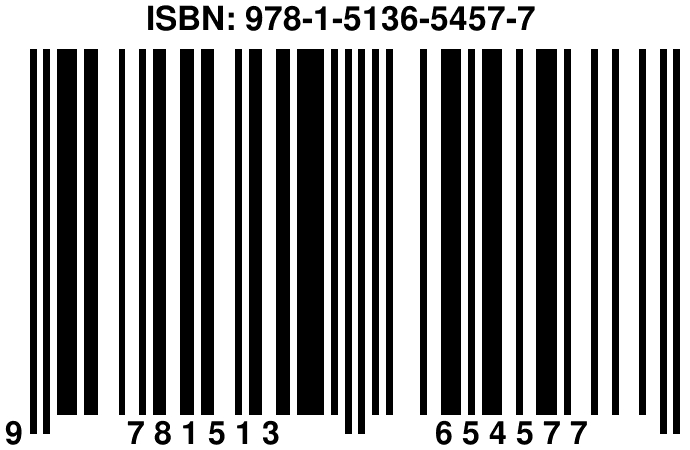
\includegraphics[width=0.9\linewidth]{misc/ALTAY19-ISBN-9781513654577}

\bibliography{book.bib,packages.bib}


\end{document}
